% Options for packages loaded elsewhere
% Options for packages loaded elsewhere
\PassOptionsToPackage{unicode}{hyperref}
\PassOptionsToPackage{hyphens}{url}
\PassOptionsToPackage{dvipsnames,svgnames,x11names}{xcolor}
%
\documentclass[
  11pt,
  a4paper,
]{report}
\usepackage{xcolor}
\usepackage[top=2.5cm,bottom=2.5cm,left=2.5cm,right=2.5cm]{geometry}
\usepackage{amsmath,amssymb}
\setcounter{secnumdepth}{2}
\usepackage{iftex}
\ifPDFTeX
  \usepackage[T1]{fontenc}
  \usepackage[utf8]{inputenc}
  \usepackage{textcomp} % provide euro and other symbols
\else % if luatex or xetex
  \usepackage{unicode-math} % this also loads fontspec
  \defaultfontfeatures{Scale=MatchLowercase}
  \defaultfontfeatures[\rmfamily]{Ligatures=TeX,Scale=1}
\fi
\usepackage{lmodern}
\ifPDFTeX\else
  % xetex/luatex font selection
\fi
% Use upquote if available, for straight quotes in verbatim environments
\IfFileExists{upquote.sty}{\usepackage{upquote}}{}
\IfFileExists{microtype.sty}{% use microtype if available
  \usepackage[]{microtype}
  \UseMicrotypeSet[protrusion]{basicmath} % disable protrusion for tt fonts
}{}
\usepackage{setspace}
\makeatletter
\@ifundefined{KOMAClassName}{% if non-KOMA class
  \IfFileExists{parskip.sty}{%
    \usepackage{parskip}
  }{% else
    \setlength{\parindent}{0pt}
    \setlength{\parskip}{6pt plus 2pt minus 1pt}}
}{% if KOMA class
  \KOMAoptions{parskip=half}}
\makeatother

\usepackage{color}
\usepackage{fancyvrb}
\newcommand{\VerbBar}{|}
\newcommand{\VERB}{\Verb[commandchars=\\\{\}]}
\DefineVerbatimEnvironment{Highlighting}{Verbatim}{commandchars=\\\{\}}
% Add ',fontsize=\small' for more characters per line
\usepackage{framed}
\definecolor{shadecolor}{RGB}{241,243,245}
\newenvironment{Shaded}{\begin{snugshade}}{\end{snugshade}}
\newcommand{\AlertTok}[1]{\textcolor[rgb]{0.68,0.00,0.00}{#1}}
\newcommand{\AnnotationTok}[1]{\textcolor[rgb]{0.37,0.37,0.37}{#1}}
\newcommand{\AttributeTok}[1]{\textcolor[rgb]{0.40,0.45,0.13}{#1}}
\newcommand{\BaseNTok}[1]{\textcolor[rgb]{0.68,0.00,0.00}{#1}}
\newcommand{\BuiltInTok}[1]{\textcolor[rgb]{0.00,0.23,0.31}{#1}}
\newcommand{\CharTok}[1]{\textcolor[rgb]{0.13,0.47,0.30}{#1}}
\newcommand{\CommentTok}[1]{\textcolor[rgb]{0.37,0.37,0.37}{#1}}
\newcommand{\CommentVarTok}[1]{\textcolor[rgb]{0.37,0.37,0.37}{\textit{#1}}}
\newcommand{\ConstantTok}[1]{\textcolor[rgb]{0.56,0.35,0.01}{#1}}
\newcommand{\ControlFlowTok}[1]{\textcolor[rgb]{0.00,0.23,0.31}{\textbf{#1}}}
\newcommand{\DataTypeTok}[1]{\textcolor[rgb]{0.68,0.00,0.00}{#1}}
\newcommand{\DecValTok}[1]{\textcolor[rgb]{0.68,0.00,0.00}{#1}}
\newcommand{\DocumentationTok}[1]{\textcolor[rgb]{0.37,0.37,0.37}{\textit{#1}}}
\newcommand{\ErrorTok}[1]{\textcolor[rgb]{0.68,0.00,0.00}{#1}}
\newcommand{\ExtensionTok}[1]{\textcolor[rgb]{0.00,0.23,0.31}{#1}}
\newcommand{\FloatTok}[1]{\textcolor[rgb]{0.68,0.00,0.00}{#1}}
\newcommand{\FunctionTok}[1]{\textcolor[rgb]{0.28,0.35,0.67}{#1}}
\newcommand{\ImportTok}[1]{\textcolor[rgb]{0.00,0.46,0.62}{#1}}
\newcommand{\InformationTok}[1]{\textcolor[rgb]{0.37,0.37,0.37}{#1}}
\newcommand{\KeywordTok}[1]{\textcolor[rgb]{0.00,0.23,0.31}{\textbf{#1}}}
\newcommand{\NormalTok}[1]{\textcolor[rgb]{0.00,0.23,0.31}{#1}}
\newcommand{\OperatorTok}[1]{\textcolor[rgb]{0.37,0.37,0.37}{#1}}
\newcommand{\OtherTok}[1]{\textcolor[rgb]{0.00,0.23,0.31}{#1}}
\newcommand{\PreprocessorTok}[1]{\textcolor[rgb]{0.68,0.00,0.00}{#1}}
\newcommand{\RegionMarkerTok}[1]{\textcolor[rgb]{0.00,0.23,0.31}{#1}}
\newcommand{\SpecialCharTok}[1]{\textcolor[rgb]{0.37,0.37,0.37}{#1}}
\newcommand{\SpecialStringTok}[1]{\textcolor[rgb]{0.13,0.47,0.30}{#1}}
\newcommand{\StringTok}[1]{\textcolor[rgb]{0.13,0.47,0.30}{#1}}
\newcommand{\VariableTok}[1]{\textcolor[rgb]{0.07,0.07,0.07}{#1}}
\newcommand{\VerbatimStringTok}[1]{\textcolor[rgb]{0.13,0.47,0.30}{#1}}
\newcommand{\WarningTok}[1]{\textcolor[rgb]{0.37,0.37,0.37}{\textit{#1}}}

\usepackage{longtable,booktabs,array}
\usepackage{calc} % for calculating minipage widths
% Correct order of tables after \paragraph or \subparagraph
\usepackage{etoolbox}
\makeatletter
\patchcmd\longtable{\par}{\if@noskipsec\mbox{}\fi\par}{}{}
\makeatother
% Allow footnotes in longtable head/foot
\IfFileExists{footnotehyper.sty}{\usepackage{footnotehyper}}{\usepackage{footnote}}
\makesavenoteenv{longtable}
\usepackage{graphicx}
\makeatletter
\newsavebox\pandoc@box
\newcommand*\pandocbounded[1]{% scales image to fit in text height/width
  \sbox\pandoc@box{#1}%
  \Gscale@div\@tempa{\textheight}{\dimexpr\ht\pandoc@box+\dp\pandoc@box\relax}%
  \Gscale@div\@tempb{\linewidth}{\wd\pandoc@box}%
  \ifdim\@tempb\p@<\@tempa\p@\let\@tempa\@tempb\fi% select the smaller of both
  \ifdim\@tempa\p@<\p@\scalebox{\@tempa}{\usebox\pandoc@box}%
  \else\usebox{\pandoc@box}%
  \fi%
}
% Set default figure placement to htbp
\def\fps@figure{htbp}
\makeatother


% definitions for citeproc citations
\NewDocumentCommand\citeproctext{}{}
\NewDocumentCommand\citeproc{mm}{%
  \begingroup\def\citeproctext{#2}\cite{#1}\endgroup}
\makeatletter
 % allow citations to break across lines
 \let\@cite@ofmt\@firstofone
 % avoid brackets around text for \cite:
 \def\@biblabel#1{}
 \def\@cite#1#2{{#1\if@tempswa , #2\fi}}
\makeatother
\newlength{\cslhangindent}
\setlength{\cslhangindent}{1.5em}
\newlength{\csllabelwidth}
\setlength{\csllabelwidth}{3em}
\newenvironment{CSLReferences}[2] % #1 hanging-indent, #2 entry-spacing
 {\begin{list}{}{%
  \setlength{\itemindent}{0pt}
  \setlength{\leftmargin}{0pt}
  \setlength{\parsep}{0pt}
  % turn on hanging indent if param 1 is 1
  \ifodd #1
   \setlength{\leftmargin}{\cslhangindent}
   \setlength{\itemindent}{-1\cslhangindent}
  \fi
  % set entry spacing
  \setlength{\itemsep}{#2\baselineskip}}}
 {\end{list}}
\usepackage{calc}
\newcommand{\CSLBlock}[1]{\hfill\break\parbox[t]{\linewidth}{\strut\ignorespaces#1\strut}}
\newcommand{\CSLLeftMargin}[1]{\parbox[t]{\csllabelwidth}{\strut#1\strut}}
\newcommand{\CSLRightInline}[1]{\parbox[t]{\linewidth - \csllabelwidth}{\strut#1\strut}}
\newcommand{\CSLIndent}[1]{\hspace{\cslhangindent}#1}



\setlength{\emergencystretch}{3em} % prevent overfull lines

\providecommand{\tightlist}{%
  \setlength{\itemsep}{0pt}\setlength{\parskip}{0pt}}



 


\usepackage{booktabs}
\usepackage{longtable}
\usepackage{array}
\usepackage{multirow}
\usepackage{wrapfig}
\usepackage{float}
\usepackage{colortbl}
\usepackage{pdflscape}
\usepackage{tabu}
\usepackage{threeparttable}
\usepackage{threeparttablex}
\usepackage[normalem]{ulem}
\usepackage{makecell}
\usepackage{xcolor}
\usepackage{pmboxdraw}
\newcommand{\CRANpkg}[1]{\textsf{#1}}
\usepackage{amsmath}
\usepackage{float}
\usepackage{hyperref}
\usepackage[utf8]{inputenc}
\usepackage{bm}
\def\tightlist{}
\usepackage{setspace}
\newcommand\pD{$p\text{-}D$}
\newcommand\kD{$k\text{-}D$}
\newcommand\dD{$d\text{-}D$}
\newcommand\gD{$2\text{-}D$}
\newcommand\hD{$4\text{-}D$}
\newcommand{\twoD}{$2\text{-}D$}
\newcommand\tD{$3\text{-}D$}
\newcommand\fD{$4\text{-}D$}
\newcommand\sD{$7\text{-}D$}
\usepackage{bm}
\newcommand{\mathbfit}[1]{\bm{#1}}
\makeatletter
\@ifpackageloaded{bookmark}{}{\usepackage{bookmark}}
\makeatother
\makeatletter
\@ifpackageloaded{caption}{}{\usepackage{caption}}
\AtBeginDocument{%
\ifdefined\contentsname
  \renewcommand*\contentsname{Table of contents}
\else
  \newcommand\contentsname{Table of contents}
\fi
\ifdefined\listfigurename
  \renewcommand*\listfigurename{List of Figures}
\else
  \newcommand\listfigurename{List of Figures}
\fi
\ifdefined\listtablename
  \renewcommand*\listtablename{List of Tables}
\else
  \newcommand\listtablename{List of Tables}
\fi
\ifdefined\figurename
  \renewcommand*\figurename{Figure}
\else
  \newcommand\figurename{Figure}
\fi
\ifdefined\tablename
  \renewcommand*\tablename{Table}
\else
  \newcommand\tablename{Table}
\fi
}
\@ifpackageloaded{float}{}{\usepackage{float}}
\floatstyle{ruled}
\@ifundefined{c@chapter}{\newfloat{codelisting}{h}{lop}}{\newfloat{codelisting}{h}{lop}[chapter]}
\floatname{codelisting}{Listing}
\newcommand*\listoflistings{\listof{codelisting}{List of Listings}}
\makeatother
\makeatletter
\makeatother
\makeatletter
\@ifpackageloaded{caption}{}{\usepackage{caption}}
\@ifpackageloaded{subcaption}{}{\usepackage{subcaption}}
\makeatother
\usepackage{bookmark}
\IfFileExists{xurl.sty}{\usepackage{xurl}}{} % add URL line breaks if available
\urlstyle{same}
\hypersetup{
  pdftitle={New Interactive Visual Tools and Statistical Methodology for Selecting and Evaluating Non-linear Dimension Reduction Layouts of High-dimensional Data},
  pdfauthor={Piyadi Gamage Jayani Lakshika},
  colorlinks=true,
  linkcolor={blue},
  filecolor={Maroon},
  citecolor={Blue},
  urlcolor={Blue},
  pdfcreator={LaTeX via pandoc}}

%% CAPTIONS
\usepackage{caption}
\DeclareCaptionStyle{italic}[justification=centering]
 {labelfont={bf},textfont={it},labelsep=colon}
\captionsetup[figure]{style=italic,format=hang,singlelinecheck=true}
\captionsetup[table]{style=italic,format=hang,singlelinecheck=true}

%% FONT
\usepackage{bera}
\usepackage[charter]{mathdesign}
\usepackage[scale=0.9]{sourcecodepro}
\usepackage[lf,t]{FiraSans}
\usepackage{fontawesome}

%% HEADERS AND FOOTERS
\usepackage{fancyhdr}
\pagestyle{fancy}
\rfoot{\Large\sffamily\raisebox{-0.1cm}{\textbf{\thepage}}}
\makeatletter
\lhead{\textsf{\expandafter{\@title}}}
\makeatother
\rhead{}
\cfoot{}
\setlength{\headheight}{15pt}
\renewcommand{\headrulewidth}{0.4pt}
\renewcommand{\footrulewidth}{0.4pt}
\fancypagestyle{plain}{%
\fancyhf{} % clear all header and footer fields
\fancyfoot[C]{\sffamily\thepage} % except the center
\renewcommand{\headrulewidth}{0pt}
\renewcommand{\footrulewidth}{0pt}}

%% MATHS
\usepackage{bm,amsmath}
\allowdisplaybreaks

%% GRAPHICS
\makeatletter
\def\fps@figure{htbp}
\makeatother
\setcounter{topnumber}{2}
\setcounter{bottomnumber}{2}
\setcounter{totalnumber}{4}
\renewcommand{\topfraction}{0.85}
\renewcommand{\bottomfraction}{0.85}
\renewcommand{\textfraction}{0.15}
\renewcommand{\floatpagefraction}{0.8}
\graphicspath{{figures/}}

%% SECTION TITLES
\usepackage[compact,sf,bf]{titlesec}
\titleformat*{\section}{\Large\sf\bfseries}
\titleformat*{\subsection}{\large\sf\bfseries}
\titleformat*{\subsubsection}{\sf\bfseries}
\titlespacing{\section}{0pt}{*5}{*1}
\titlespacing{\subsection}{0pt}{*2}{*0.2}
\titlespacing{\subsubsection}{0pt}{*1}{*0.1}

%% TABLES
\usepackage{booktabs,tabu}

%% BIBLIOGRAPHY.

\makeatletter
\@ifpackageloaded{biblatex}{
\ExecuteBibliographyOptions{bibencoding=utf8,minnames=1,maxnames=3, maxbibnames=99,dashed=false,terseinits=true,giveninits=true,uniquename=false,uniquelist=false,doi=false, isbn=false,url=true,sortcites=false}
\DeclareFieldFormat{url}{\texttt{\url{#1}}}
\DeclareFieldFormat[article]{pages}{#1}
\DeclareFieldFormat[inproceedings]{pages}{\lowercase{pp.}#1}
\DeclareFieldFormat[incollection]{pages}{\lowercase{pp.}#1}
\DeclareFieldFormat[article]{volume}{\mkbibbold{#1}}
\DeclareFieldFormat[article]{number}{\mkbibparens{#1}}
\DeclareFieldFormat[article]{title}{\MakeCapital{#1}}
\DeclareFieldFormat[article]{url}{}
\DeclareFieldFormat[inproceedings]{title}{#1}
\DeclareFieldFormat{shorthandwidth}{#1}
\usepackage{xpatch}
\xpatchbibmacro{volume+number+eid}{\setunit*{\adddot}}{}{}{}
% Remove In: for an article.
\renewbibmacro{in:}{%
  \ifentrytype{article}{}{%
  \printtext{\bibstring{in}\intitlepunct}}}
\AtEveryBibitem{\clearfield{month}}
\AtEveryCitekey{\clearfield{month}}
\DeclareDelimFormat[cbx@textcite]{nameyeardelim}{\addspace}
\renewcommand*{\finalnamedelim}{\addspace\&\space}
}{}
\makeatother


\hypersetup{
     pdfcreator={Quarto -> pandoc -> LaTeX -> pdf}
}


%% PAGE BREAKING to avoid widows and orphans
\clubpenalty = 2000
\widowpenalty = 2000
\usepackage{microtype}
\def\maketitle{
\pagenumbering{roman}
{\sf\thispagestyle{empty}%
  \null\vskip-.4cm%
  \centerline{
\includegraphics[width=12cm]{monash-logo}}
  \vspace*{4cm}
  \begin{center}\fontsize{24}{28}\sf
     \textbf{New Interactive Visual Tools and Statistical Methodology
for Selecting and Evaluating Non-linear Dimension Reduction Layouts of
High-dimensional Data}\\[2cm]
     \fontsize{18}{20}\sf Piyadi Gamage Jayani Lakshika\\[0.2cm]
     \fontsize{13}{15}\sf B.Sc. (Hons) in Statistics, University of Sri
Jayewardenepura (USJ), Sri Lanka
     \vfill
     \fontsize{13}{15}\sf A thesis submitted for the degree of\\ Doctor
of Philosophy\\ at Monash University in \number\the\year\\
     Department of Econometrics \& Business Statistics
  \end{center}
  \newpage\mbox{}\thispagestyle{empty}\newpage
}
}

% Title and date

\title{New Interactive Visual Tools and Statistical Methodology for
Selecting and Evaluating Non-linear Dimension Reduction Layouts of
High-dimensional Data}
\date{}
\begin{document}
\maketitle

\renewcommand*\contentsname{Table of contents}
{
\hypersetup{linkcolor=}
\setcounter{tocdepth}{1}
\tableofcontents
}

\setstretch{1.5}
\bookmarksetup{startatroot}

\chapter*{Copyright notice}\label{copyright-notice}
\addcontentsline{toc}{chapter}{Copyright notice}

\markboth{Copyright notice}{Copyright notice}

Produced on 14 November 2025.

© Piyadi Gamage Jayani Lakshika (2025).

I certify that I have made all reasonable efforts to secure copyright
permissions for third-party content included in this thesis and have not
knowingly added copyright content to my work without the owner's
permission.

\clearpage\pagenumbering{arabic}\setcounter{page}{1}

\bookmarksetup{startatroot}

\chapter*{Abstract}\label{abstract}
\addcontentsline{toc}{chapter}{Abstract}

\markboth{Abstract}{Abstract}

High-dimensional data are increasingly common across many scientific
fields, driven by advances in data collection technologies. However,
visualizing and interpreting such data pose significant challenges due
to the difficulty of perceiving structures beyond two dimensions.
Dimension reduction methods are widely used to create visual summaries
of high-dimensional data. While linear approaches such as principal
component analysis are effective for simple structures, they often fail
to capture complex, nonlinear relationships. Nonlinear dimension
reduction (NLDR) techniques address this limitation by applying
nonlinear transformations to produce low-dimensional representations
that reveal intricate patterns within the data. However, NLDR methods
vary in how they distort or preserve structure, and their results can be
misleading without appropriate diagnostic tools. However, the
effectiveness of NLDR methods can vary depending on the chosen method
and hyper-parameters, often resulting in representations that differ
widely in accuracy and can be misleading without proper diagnostic
tools. The main objective of this research is to develop new methods and
software tools to diagnose, evaluate, and interpret NLDR results in
relation to the true high-dimensional data structure.

This research presents five original contributions. The first
contribution (\hyperref[sec-first-paper]{Chapter 2}) introduces a new
method for visualizing how NLDR warps data. This method improves the
diagnostics of NLDR techniques. The second contribution
(\hyperref[sec-third-paper]{Chapter 3}) involves implementing the method
introduced in \hyperref[sec-first-paper]{Chapter 2} as an R package,
\texttt{quollr}. The third contribution
(\hyperref[sec-fourth-paper]{Chapter 4}) introduces an R package,
\texttt{cardinalR} designed to generate high-dimensional clustering data
structures, with features such as adding noise dimensions and background
noise. The fourth contribution (\hyperref[sec-second-paper]{Chapter 5})
provides evidence in identification of clusters at various distances
when observing NLDR representation and the tour view of high-dimensional
data. This finding is based on a human subject experiment that explores
both the perception and misperception of NLDR representations. Finally,
the fifth contribution (\hyperref[sec-fifth-paper]{Chapter 6}) provides
a Shiny app that offers a user-friendly interface for analysts to obtain
the most accurate NLDR representation. Overall, this work advances the
field of diagnosing NLDR by improving the visualization of
high-dimensional data.

\bookmarksetup{startatroot}

\chapter*{Declaration}\label{declaration}
\addcontentsline{toc}{chapter}{Declaration}

\markboth{Declaration}{Declaration}

I hereby declare that this thesis contains no material which has been
accepted for the award of any other degree or diploma at any university
or equivalent institution and that, to the best of my knowledge and
belief, this thesis contains no material previously published or written
by another person, except where due reference is made in the text of the
thesis.

This thesis includes one original papers published in a peer reviewed
journal and four unpublished papers. The core theme of the thesis is to
``develop methods and software to evaluate and understand non-linear
dimension reduction methods''. The ideas, development and writing up of
all the papers in the thesis were the principal responsibility of
myself, the student, working within the Department of Econometrics and
Business Statistics under the supervision of Professor Dianne Cook, Dr
Paul Harrison (MGBP, BDInstitute), Dr Michael Lydeamore, and Dr Thiyanga
S. Talagala (University of Sri Jayewardenepura).

The inclusion of co-authors reflects the fact that the work came from
active collaboration between researchers and acknowledges input into
team-based research. In the case of \hyperref[sec-first-paper]{Chapter
2}, \hyperref[sec-third-paper]{Chapter 3},
\hyperref[sec-fourth-paper]{Chapter 4}, and,
\hyperref[sec-fifth-paper]{Chapter 6}, my contribution to the work
involved the following:

\begingroup\fontsize{10}{12}\selectfont

\begin{longtable*}[t]{>{\raggedleft\arraybackslash}p{1.2cm}>{\raggedright\arraybackslash}p{3cm}>{\raggedright\arraybackslash}p{3.5cm}>{\raggedright\arraybackslash}p{2.5cm}>{\raggedright\arraybackslash}p{2.4cm}>{\raggedright\arraybackslash}p{1.3cm}}
\toprule
\multicolumn{1}{>{\raggedright\arraybackslash}p{1.2cm}}{\textbf{Chapter}} & \multicolumn{1}{>{\raggedright\arraybackslash}p{3cm}}{\textbf{Publication title}} & \multicolumn{1}{>{\raggedright\arraybackslash}p{3.5cm}}{\textbf{Status}} & \multicolumn{1}{>{\raggedright\arraybackslash}p{2.5cm}}{\textbf{Student contribution}} & \multicolumn{1}{>{\raggedright\arraybackslash}p{2.4cm}}{\textbf{Co-authors contribution}} & \multicolumn{1}{>{\raggedright\arraybackslash}p{1.3cm}}{\textbf{Coauthors are Monash students}}\\
\midrule
\endfirsthead
\multicolumn{6}{@{}l}{\textit{(continued)}}\\
\toprule
\multicolumn{1}{>{\raggedright\arraybackslash}p{1.2cm}}{\textbf{Chapter}} & \multicolumn{1}{>{\raggedright\arraybackslash}p{3cm}}{\textbf{Publication title}} & \multicolumn{1}{>{\raggedright\arraybackslash}p{3.5cm}}{\textbf{Status}} & \multicolumn{1}{>{\raggedright\arraybackslash}p{2.5cm}}{\textbf{Student contribution}} & \multicolumn{1}{>{\raggedright\arraybackslash}p{2.4cm}}{\textbf{Co-authors contribution}} & \multicolumn{1}{>{\raggedright\arraybackslash}p{1.3cm}}{\textbf{Coauthors are Monash students}}\\
\midrule
\endhead

\endfoot
\bottomrule
\endlastfoot
2 &  & Revised and resubmitted in the Journal of Computational and Graphical Statistics & 80\%  Concept, Analysis, Software, Writing &  & No\\
3 &  & Submitted in the R Journal & 80\%  Concept, Analysis, Software, Writing &  & No\\
4 &  & Submitted in the R Journal & 80\%  Concept, Analysis, Software, Writing &  & No\\
6 &  & Submitted in the Oxford Academic (Bioinformatics Advances) & 80\%  Concept, Analysis, Software, Writing &  & No\\*
\end{longtable*}
\endgroup{}

Chapters 3 is planned for submission to peer-reviewed journal.

\clearpage

To ensure the clarity and coherence of the written content, artificial
intelligence tools were employed to assist in smoothing and refining the
language throughout the thesis.

This thesis uses American spelling, as that's the style followed by the
journals where the work will be submitted or published.

I have renumbered sections of submitted papers in order to generate a
consistent presentation within the thesis.

\textbf{Student name}: Piyadi Gamage Jayani Lakshika

\textbf{Student signature}:

\textbf{Date}: 13th January 2026

I hereby certify that the above declaration correctly reflects the
nature and extent of the student's and co-authors' contributions to this
work. In instances where I am not the responsible author I have
consulted with the responsible author to agree on the respective
contributions of the authors.

\textbf{Main Supervisor name}: Dianne Cook

\textbf{Main Supervisor signature}:

\textbf{Date}: 13th January 2026

\bookmarksetup{startatroot}

\chapter*{Acknowledgements}\label{acknowledgements}
\addcontentsline{toc}{chapter}{Acknowledgements}

\markboth{Acknowledgements}{Acknowledgements}

This thesis would have never been a success without the guidance,
encouragement, and support of my supervisors, family, and friends. This
note is to show my gratitude to them.

First, I would like to sincerely thank my supervisors Professor Dianne
Cook, Dr Paul Harrison, Dr Michael Lydeamore, and Dr Thiyanga S.
Talagala for being incredible supervisors and mentors. Their endless
enthusiasm for research, productivity, and wealth of knowledge has
motivated me throughout my Ph.D.~at Monash university. No matter how
busy they were, they always kept the doors open to welcome me, whenever
I needed their help. I believe that they are the best supervisors I
could ever find in my life long research journey. Thank you for
believing in my ability to navigate difficulties, even when I doubted
myself. I am immensely grateful and honoured to have worked under
guidance of you all. Your expertise, way of thinking, and leadership
will continue to inspire me now and always.

I gratefully acknowledge the constructive feedback, suggestions, and
encouragement I received from my PhD milestone evaluation panel members:
Professor Catherine Forbes, Professor Xibin Zhang, Associate Professor
Ruben Loaiza Maya, Dr Jessica Leung, Dr Shanika Wickramasuriya, and Dr
Kate Saunders. Special thanks go to Professor Catherine Forbes, and
Professor Xibin Zhang for being outstanding PhD directors and for their
immense support throughout my candidature. I am also thankful to
Professor Mervyn Silvapulle and Emeritus Professor Donald Poskitt, who
taught our PhD coursework units during the first year of the programme.

I am thankful to Monash University, Australia, for this invaluable
opportunity to pursue my PhD at such a prestigious institution. The
exposure and experiences I gained over the years at Monash have been
immense. I am particularly grateful for the financial support provided
through the Co-funded Graduate Research Scholarship and the Monash
Business School Co-Funded Graduate Research Scholarship, which enabled
me to concentrate fully on my research. I am also thankful for the
financial assistance provided to attend international conferences and
visiting some invaluable mentors in the USA and Austria. I take this
opportunity to express my sincere gratitude to all other academic and
administrative staff members of the Department of Econometric and
Business Statistics at Monash University.

I would like to sincerely thank Emeritus Professor Gael Martin, who,
together with Professor Rob Hyndman, welcomed me into the department at
the time of my application. I also thank Professor George Athanasopoulos
for his generous assistance in making it possible for me to complete my
visit to the USA. My heartfelt thanks go as well to Professor Brett
Inder, Associate Professor Christo Karuna, and Professor Xueyan Zhao,
whose warm smiles, encouragement, and constant support have been
invaluable in helping me to complete this journey.

I would also like to thank Professor Heike Hofmann, Associate Professor
Susan VanderPlas, Associate Professor Ursula Laa, Associate Professor
Natalia da Silva, and Professor Eun-Kyung, whom I had the privilege of
visiting during my PhD journey. Their generosity in providing
opportunities, their guidance in improving my work, and their endless
care and kindness have meant a great deal to me. I am also grateful to
the University of Nebraska--Lincoln, USA and the University of Natural
Resources and Life Sciences, Vienna, Austria, for warmly hosting me
during these visits.

I acknowledge the use of \href{https://app.grammarly.com/}{Grammarly}
and \href{https://chatgpt.com/}{ChatGPT} for grammar and spelling
checks, which helped improve the accuracy of my writing.

I remember with gratitude, the University of Sri Jayewardenepura, Sri
Lanka, for paving the way for my academic journey. I am especially
grateful to my undergraduate research supervisor, Dr Thiyanga S.
Talagala, for sparking my interest in visualisation, and for broadening
my academic horizons through her wisdom and mentorship. Without her
guidance, I would never have thought to begin this journey, and I remain
deeply grateful for that. I am also grateful to Sigithi Kindergarten,
Weligama, Sri Sumangala Balika Vidyalaya, Weligama, and Sujatha
Vidyalaya, Matara, Sri Lanka, where I received my early, primary, and
secondary education. I extend my heartfelt thanks to all my teachers and
private tutors, who continue to check on me even today. The lessons and
challenges from those years made me stronger and more resilient, which
proved invaluable during my PhD journey.

Chapter 2 is being revised for the \textbf{Journal of Computational and
Graphical Statistics}. I take this opportunity to thank the two
anonymous reviewers for their constructive comments. I presented my
research work at \(12^{th}\)-Conference of the Asian Regional Section of
the International Association for Statistical Computing (IASC-ARS 2023)
(Wollongon, Australia), Australian Statistical Conference (ASC 2023)
(Wollongon, Australia), Bioinformatics Seminar 2024, Victorian branch of
the Australian and New Zealand Industrial and Applied Mathematics
Society (VicANZIAM) 2024 (RMIT university, Melbourne, Australia),
Faculty of BusEco Three Minute Thesis (3MT) competition 2024, useR! 2024
(Salzburg, Austria), Graphics Group Presentation 2024 (Nebraska, USA),
UNO Data Science Club 2024 (Omaha, USA), Joint Statistical Meetings
(JSM) 2025 (Nashville, USA), useR! 2025 (Durham, USA), Biometrics in the
Bush Capital (BIBC2025) (Canberra, Australia), and Australian
Statistical Conference (ASC 2025) (Perth, Western Australia). I would
like to thank the participants of these seminars, research groups, and
the conferences for their valuable comments.

I am deeply grateful to my extended family here in Melbourne Nuwani and
Rehan, Heshani and Kanishka, and Shanika (also became my gym partner),
who not only stood by me during difficult times and but constant
listeners. My heartfelt thanks also go to Chaya and Supun, Himasha and
Danushka, and Hiruni, for their genuine friendship and unwavering
support.

I am thankful to my fellow PhD students at Monash for making this
journey such a memorable experience. Special appreciation goes to my
``Numbats family'' Patrick, Mitch, Fin, Sherry, Cynthia, Harriet,
Janith, Kris, David, and Hannah for the camaraderie and encouragement. I
also treasure the many conversations with Nimni and Gayani during office
hours, which brought lightness and motivation to my days. To my office
mates: Shelly, Elvis, Floyd, Cash, Minh, and Vis thank you for creating
a supportive and welcoming environment. I am especially grateful to
Dr.~Xiaoqian, both an office mate and a wonderful roommate during
conference trips, for sharing this journey with me.

My sincere thanks go to Dovini and Vihanga for their help during my
English test and the application process to Australia, and to the MIG
family for their kindness and support throughout my PhD. I also extend
my gratitude to Danusha, Kalani, Narmada, Malith, and all the friends I
met during my visit to the University of Nebraska, USA, who made that
experience so enriching. I will never forget the kindness of Dilmi and
Nishadi, who welcomed me on my very first day in Melbourne, picked me
up, and helped me settle into a new life. I remain truly grateful for
their generosity. I am grateful to Pabasara, Vindula, Amaya, Nirmitha,
and Malinda for being wonderful friends from my university days until
now, and for continuing to support me through the difficult moments of
this journey. I also sincerely thank Kavishka, Dinith, Sonal, Thilina,
and Tharaka for their enduring friendship and encouragement throughout
this time. A special thanks to Paton, Michael's dog, whose wagging tail
and joyful spirit always lifted my mood.

Last, but by no means least, I would like to thank my family members. I
am truly grateful to my parents for their unconditional selfless love,
care, and sacrifices that they made to make my life better. Your
inspiration and guidance always kept me motivated to perceive better
achievements in my life. I am fortunate to be your daughter. I would
also like to thank my sister, my brother, and my sister-in-law for their
unconditional love, understanding, and moral support both in this
academic journey and in life. No matter how I stumble, you have always
lifted me up and reminded me of my worth. Amma, Thaththa, Nangi, Malli
and Podi nangi I am endlessly grateful for you, beyond words, beyond
life, and beyond everything.

This journey was never mine alone, and for that, I am eternally
grateful!

\clearpage\pagenumbering{arabic}\setcounter{page}{0}

\bookmarksetup{startatroot}

\chapter{Introduction}\label{sec-intro}

A high-dimensional dataset is one in which each observation is described
by many features, or dimensions, often with associations among them.
Such data are increasingly common in fields like bioinformatics,
ecology, and forensic science. For example, \textbf{CITE-seq data}
(\citeproc{ref-hao2021}{Hao et al. 2021}) simultaneously records RNA
expression and protein markers for individual cells, resulting in
high-dimensional dataset. Working with high-dimensional data poses
considerable challenges due to the difficulty in visualizing beyond two
dimensions (\citeproc{ref-jia2022}{Jia et al. 2022}). High-dimensional
data also presents difficulties for model fitting
(\citeproc{ref-johnstone2009}{Johnstone and Titterington 2009}), both
computationally and with interpretation, each of which benefits from
visualization.

To create visual representations of high-dimensional data, it is common
to apply \textbf{dimension reduction} techniques. One established
approach is \textbf{linear projection}, where high-dimensional points
are represented as linear combinations of the original features.
\textbf{Principal Component Analysis (PCA)} (for an overview see
Jolliffe (\citeproc{ref-jolliffe2011}{2011})) is the most familiar
method, identifying directions of maximum variance. Extending this idea,
\textbf{tours} (\citeproc{ref-lee2021}{Lee et al. 2021}) provide dynamic
sequences of linear projections, giving views from multiple angles to
help reveal hidden structure. Tour methods are implemented in R packages
such as \texttt{tourr} (\citeproc{ref-wickham2011}{Wickham et al.
2011}), \texttt{langevitour} (\citeproc{ref-harisson2024}{Harrison
2023}), and \texttt{detourr} (\citeproc{ref-hart2022}{Hart and Wang
2022}). A key advantage of linear projections is that they preserve the
geometric relationships of the original data, they do not introduce
distortion. However, linear projections can become cluttered, and global
structure may obscure local detail. Furthermore, \emph{piling}
(\citeproc{ref-laa2022}{Laa et al. 2022}) where points concentrate in
the center of projections can mask important variation.

To overcome these limitations, analysts frequently turn to
\textbf{nonlinear dimension reduction (NLDR)} methods such as
t-distributed stochastic neighbor embedding (tSNE)
(\citeproc{ref-laurens2008}{Maaten and Hinton 2008}), uniform manifold
approximation and projection (UMAP) (\citeproc{ref-leland2018}{McInnes
et al. 2018}), potential of heat-diffusion for affinity-based trajectory
embedding (PHATE) algorithm (\citeproc{ref-moon2019}{Moon et al. 2019}),
large-scale dimensionality reduction using triplets (TriMAP)
(\citeproc{ref-amid2022}{Amid and Warmuth 2022}), and pairwise
controlled manifold approximation (PaCMAP)
(\citeproc{ref-yingfan2021}{Wang et al. 2021}). The methods tSNE, UMAP,
TriMAP and PaCMAP can be considered for producing the \kD{}
representation by minimizing the divergence between two inter-point
distance distributions. PHATE is an example of a diffusion process
spreading to capture geometric shapes, that include both global and
local structure. (See Coifman et al. (\citeproc{ref-coifman2005}{2005})
for an explanation of diffusion processes.) These methods are designed
to \emph{exaggerate structure}, making it easier for analysts to detect
patterns that may not be apparent through linear projections.

\begin{figure}[H]

\centering{

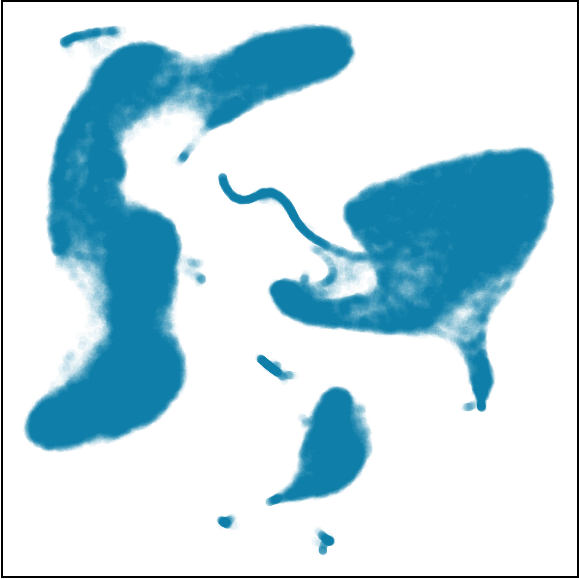
\includegraphics[width=1\linewidth,height=\textheight,keepaspectratio]{chapters/01-chap1_files/figure-pdf/fig-NLDR-variety-intro-1.pdf}

}

\caption{\label{fig-NLDR-variety-intro}Eight different NLDR
representations of a human PBMC CITE-seq dataset (Hao et al.
(\citeproc{ref-hao2021}{2021})). Different techniques and different
hyper-parameter choices are used (\emph{(a) UMAP (n\_neighbors = 15,
min\_dist = 0.1), (b) UMAP (n\_neighbors = 54, min\_dist = 0.5), (c)
PaCMAP (n\_neighbors = 51, init = random, MN\_ratio = 0.3, FP\_ratio =
2), (d) tSNE (perplexity = 30), (e) tSNE (perplexity = 84), (f) PHATE
(knn = 5), (g) TriMAP (n\_inliers = 12, n\_outliers = 4, n\_random = 3),
(h) PaCMAP (n\_neighbors = 10, init = random, MN\_ratio = 0.5, FP\_ratio
= 2)}). Researchers may have seen any of these in their analysis of this
data, depending on their choice of method, or typical hyper-parameter
choice. Would they make different decisions downstream in the analysis
depending on which version seen? Which is the most accurate
representation of the structure in high dimensions?}

\end{figure}%

Yet this strength also introduces a critical risk: \textbf{NLDR can
hallucinate structure}, creating patterns in the low-dimensional space
that do not exist in the high-dimensional data. This issue is strikingly
illustrated in Figure~\ref{fig-NLDR-variety-intro}, where eight
different NLDR representations of the same CITE-seq dataset vary
dramatically due to differences in method or hyper-parameter choices.
Such variability raises essential questions: \emph{Which layout can be
trusted? Which accurately represents the high-dimensional data
structure(s)?}

Despite the widespread use of NLDR, there is no widely accepted or
visually interpretable framework for \textbf{diagnosing the reliability
of NLDR representations}. Analysts are left to rely on subjective
judgment when choosing and interpreting NLDR layouts, without tools to
distinguish faithful representations from artifacts. There is also a
lack of benchmark clustering datasets for testing specially NLDR
methods.

In addition to technical gaps, \textbf{little is known about how people
perceive and misperceive structure in NLDR layouts}. It is unclear how
different NLDR representations influence analysts' conclusions, or how
distortions introduced by NLDR affect decision making. Given the
critical role of visualization in high-dimensional data analysis,
understanding the human perception of NLDR representations is essential.

\section{Research Objectives}\label{research-objectives}

This thesis aims to achieve the key challenges in understanding and
evaluating NLDR methods through four main objectives:

\begin{enumerate}
\def\labelenumi{\arabic{enumi}.}
\item
  \textbf{Develop a new approach and software to evaluate NLDR
  techniques}, providing tools to assess whether low-dimensional
  representations accurately capture the high-dimensional data
  structures, using visual and quantitative diagnostics.
\item
  \textbf{Conduct a large-scale user study to explore perception and
  misperception in NLDR representations}, assessing how participants
  recognize the data structure similarly in NLDR layout compared to tour
  views. This cognitive perception experiment provides common mistakes
  made when choosing and reporting structure from NLDR representations,
  and will inform best practices for using these methods in data
  analysis.
\item
  \textbf{Generate benchmark clustering data structures in high
  dimensions with some additional properties like background noise},
  using the \texttt{cardinalR} package, to evaluate the performance of
  the algorithms like clustering, NLDR.
\item
  \textbf{Provide a platform for NLDR users}, comparing multiple NLDR
  representations and select the most reasonable one.
\end{enumerate}

\section{Contribution}\label{contribution}

This research contributes to a deeper understanding of how NLDR methods
can be evaluated and trusted in practice. It provides new tools and
software for assessment, benchmark datasets for testing algorithms, and
insights from a large-scale user study to guide effective use of NLDR in
high-dimensional data analysis.

\section{Thesis Outline}\label{thesis-outline}

The rest of the thesis is organized as follows:

Chapter~\ref{sec-first-paper} introduces an algorithm to assess the NLDR
and decide on which, if any, is the most reasonable representation of
the structure(s) present in high-dimensional data. We create a model
starting with NLDR layout that is then used to display as a wireframe in
high dimensions.

Chapter~\ref{sec-third-paper} presents the implementation of the work is
available as an R package, named \texttt{quollr}, an acronym to
``\textbf{qu}estioning how a high-dimensional \textbf{o}bject
\textbf{l}ooks in \textbf{l}ow-dimensions using \textbf{r}''
(\citeproc{ref-jayani2024a}{\textbf{jayani2024a?}}). This package also
contains a function for performing hexagonal binning using a new
approach, for saving langevitour results with a specific projection, and
link plots to understand the quirks that occur with different NLDR
techniques.

Chapter~\ref{sec-fourth-paper} proposes the R package,
\texttt{cardinalR} (\citeproc{ref-jayani2024b}{\textbf{jayani2024b?}})
(\textbf{c}ollection of v\textbf{ar}ious
high-\textbf{d}imens\textbf{i}o\textbf{nal} data structures in
\textbf{R}), which includes functions to generate high-dimensional
clustering data structures, with features such as adding noise
dimensions and background noise along with some already generated
examples.

Chapter~\ref{sec-second-paper} provides empirical evidence on how
viewers recognize structure differently when using NLDR layouts versus
the tour view, particularly with varying distances between clusters. The
findings will help clarify common mistakes made when selecting and
reporting structures based on NLDR layouts.

Chapter~\ref{sec-fifth-paper} introduces \texttt{menuraR}
(\textbf{m}onitoring \textbf{e}mbeddings of \textbf{n}onlinear
\textbf{u}nfoldings for \textbf{r}epresentation and \textbf{a}nalysis in
\textbf{R}), a Shiny web application designed to select and evaluate
NLDR layouts.

Chapter~\ref{sec-conclusion} concludes the thesis, summarizes the
contribution of the work, and discusses some future plans.

\bookmarksetup{startatroot}

\chapter{Choosing Better NLDR Layouts by Evaluating the Model in the
High-dimensional Data Space}\label{sec-first-paper}

\section{Introduction}\label{introduction}

Nonlinear dimension reduction (NLDR) is popular for making a convenient
low-dimensional (\kD{}) representation of high-dimensional (\pD{}) data
(\(k < p\)). Recently developed methods include t-distributed stochastic
neighbor embedding (tSNE) (\citeproc{ref-laurens2008}{Maaten and Hinton
2008}), uniform manifold approximation and projection (UMAP)
(\citeproc{ref-leland2018}{McInnes et al. 2018}), potential of
heat-diffusion for affinity-based trajectory embedding (PHATE) algorithm
(\citeproc{ref-moon2019}{Moon et al. 2019}), large-scale dimensionality
reduction using triplets (TriMAP)
(\citeproc{ref-amid2019}{\textbf{amid2019?}}), and pairwise controlled
manifold approximation (PaCMAP) (\citeproc{ref-yingfan2021}{Wang et al.
2021}).

However, the representation generated can vary dramatically from method
to method, choice of hyper-parameter or even random seed, as illustrate
by Figure~\ref{fig-NLDR-variety}. The specific method and
hyper-parameters used to produce each layout (see Appendix) is not
essential for the discussion. The dilemma for the analyst is which
representation to use. The choice might result in different procedures
used in the downstream analysis, or different inferential conclusions.
Various academics have expressed concerns with current practices and
procedures for choosing (e.g. Irizarry
(\citeproc{ref-irizarry2024}{2024}), Chari and Pachter
(\citeproc{ref-chari2023}{2023})). The research described here provides
new numerical and visual tools to aid with this decision.

\begin{figure}

\centering{

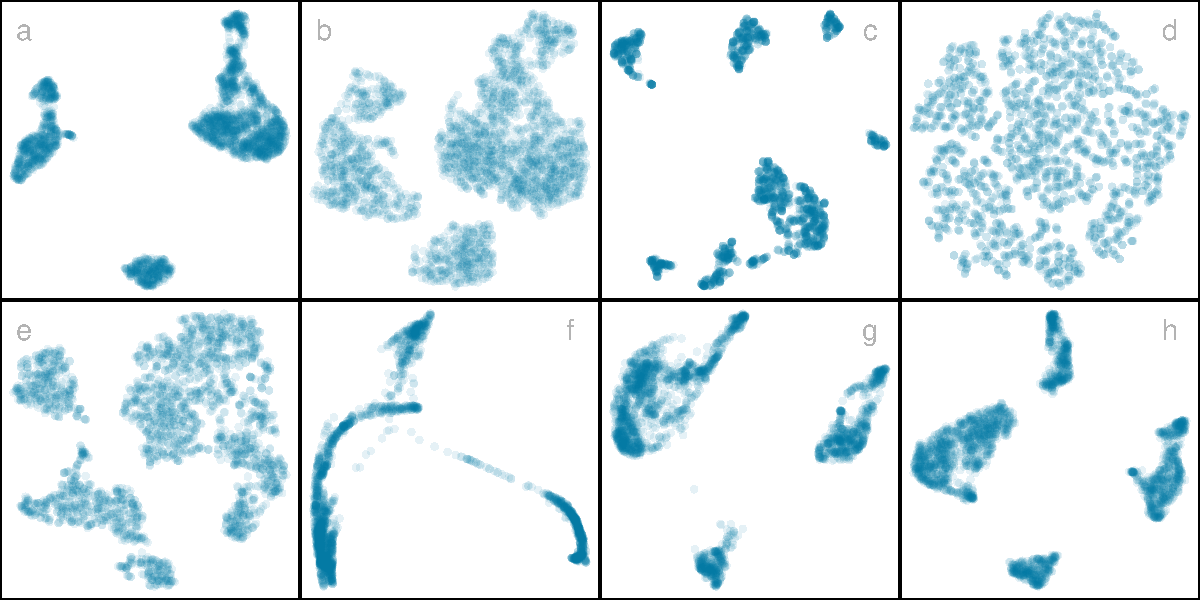
\includegraphics[width=0.8\linewidth,height=\textheight,keepaspectratio]{chapters/02-chap2_files/figure-pdf/fig-NLDR-variety-1.pdf}

}

\caption{\label{fig-NLDR-variety}Eight different NLDR representations of
the same data, produced by tSNE, UMAP, PHATE, TriMAP and PaCMAP with a
variety of hyper-parameter choices. The variety in layouts makes it
difficult to choose which best represents the data distribution.}

\end{figure}%

The paper is organized as follows. Section~\ref{sec-background} provides
a summary of the literature on NLDR, and high-dimensional data
visualization methods. Section~\ref{sec-method} contains the details of
the new methodology, including simulated data examples. In
Section~\ref{sec-bestfit}, we describe how to assess the best fit and
identify the most accurate \gD{} layout based on the proposed model
diagnostics. Two applications illustrating the use of the new
methodology for bioinformatics and image classification are in
Section~\ref{sec-applications}. Limitations and future directions are
provided in Section~\ref{sec-discussion}.

\section{Background}\label{sec-background}

Historically, low-dimensional (\kD{}) representations of
high-dimensional (\pD{}) data have been computed using multidimensional
scaling (MDS) (\citeproc{ref-kruskal1964}{Kruskal 1964}), which includes
principal components analysis (PCA) (for an overview see Jolliffe
(\citeproc{ref-jolliffe2011}{2011})). (A contemporary comprehensive
guide to MDS can be found in Borg and Groenen
(\citeproc{ref-borg2005}{2005}).) The \kD{} representation can be
considered to be a layout of points in \kD{} produced by an embedding
procedure that maps the data from \pD{}. In MDS, the \kD{} layout is
constructed by minimizing a stress function that differences distances
between points in \pD{} with potential distances between points in
\kD{}. Various formulations of the stress function result in non-metric
scaling (\citeproc{ref-saeed2018}{Saeed et al. 2018}) and isomap
(\citeproc{ref-silva2002}{Silva and Tenenbaum 2002}). Challenges in
working with high-dimensional data, including visualization, are
outlined in Johnstone and Titterington
(\citeproc{ref-johnstone2009}{2009}).

Many new methods for NLDR have emerged in recent years, all designed to
better capture specific structures potentially existing in \pD{}. Here
we focus on five currently popular techniques: tSNE, UMAP, PHATE, TriMAP
and PaCMAP. The methods tSNE, UMAP, TriMAP and PaCMAP can be considered
for producing the \kD{} representation by minimizing the divergence
between two inter-point distance distributions. PHATE is an example of a
diffusion process spreading to capture geometric shapes, that include
both global and local structure. (See Coifman et al.
(\citeproc{ref-coifman2005}{2005}) for an explanation of diffusion
processes.)

The array of layouts in Figure~\ref{fig-NLDR-variety} illustrate what
can emerge from the choices of method and hyper-parameters, and the
random seed that initiates the computation. Key structures interpreted
from these views suggest: (1) highly \textbf{separated clusters} (a, b,
e, g, h) with the number ranging from 3-6; (2) \textbf{stringy branches}
(f), and (3) \textbf{barely separated clusters} (c, d) which would
\textbf{contradict} the other representations. These contradictions
arise because these methods and hyper-parameter choices provide
different lenses on the interpoint distances in the data.

The alternative approach to visualizing the high-dimensional data is to
use linear projections. PCA is the classical approach, resulting in a
set of new variables which are linear combinations of the original
variables. Tours, defined by Asimov (\citeproc{ref-As85}{1985}), broaden
the scope by providing movies of linear projections, that provide views
the data from all directions. (See Lee et al.
(\citeproc{ref-lee2021}{2021}) for a review of tour methods.) There are
many tour algorithms implemented, with many available in the R package
\texttt{tourr} (\citeproc{ref-wickham2011}{Wickham et al. 2011}), and
versions enabling better interactivity in \texttt{langevitour}
(\citeproc{ref-harisson2024}{Harrison 2023}) and \texttt{detourr}
(\citeproc{ref-hart2022}{Hart and Wang 2022}). Linear projections are a
safe way to view high-dimensional data, because they do not warp the
space, so they are more faithful representations of the structure.
However, linear projections can be cluttered, and global patterns can
obscure local structure. The simple activity of projecting data from
\pD{} suffers from piling (\citeproc{ref-laa2022}{Laa et al. 2022}),
where data concentrates in the center of projections. NLDR is designed
to escape these issues, to exaggerate structure so that it can be
observed. But as a result NLDR can hallucinate wildly, to suggest
patterns that are not actually present in the data.

Our proposed solution is to use the tour to examine how the NLDR is
warping the space. It follows what Wickham et al.
(\citeproc{ref-wickham2015}{2015}) describes as
\emph{model-in-the-data-space}. The fitted model should be overlaid on
the data, to examine the fit relative the spread of the observations.
While this is straightforward, and commonly done when data is \gD{}, it
is also possible in \pD{}, for many models, when a tour is used.

Wickham et al. (\citeproc{ref-wickham2015}{2015}) provides several
examples of models overlaid on the data in \pD{}. In hierarchical
clustering, a representation of the dendrogrom using points and lines
can be constructed by augmenting the data with points marking merging of
clusters. Showing the movie of linear projections reveals shows how the
algorithm sequentially fitted the cluster model to the data. For linear
discriminant analysis or model-based clustering the model can be
indicated by \((p-1)\text{-}D\) ellipses. It is possible to see whether
the elliptical shapes appropriately matches the variance of the relevant
clusters, and to compare and contrast different fits. For PCA, one can
display the model (a \kD{} plane of the reduced dimension) using
wireframes of transformed cubes. Using a wireframe is the approach we
take here, to represent the NLDR model in \pD{}.

\section{Method}\label{sec-method}

\subsection{What is the NLDR model?}\label{what-is-the-nldr-model}

At first glance, thinking of NLDR as a modeling technique might seem
strange. It is a simplified representation or abstraction of a system,
process, or phenomenon in the real world. The \pD{} observations are the
realization of the phenomenon, and the \kD{} NLDR layout is the
simplified representation. Typically, \(k=2\), which is used for the
rest of this paper. From a statistical perspective we can consider the
distances between points in the \gD{} layout to be variance that the
model explains, and the (relative) difference with their distances in
\pD{} is the error, or unexplained variance. We can also imagine that
the positioning of points in \gD{} represent the fitted values, that
will have some prescribed position in \pD{} that can be compared with
their observed values. This is the conceptual framework underlying the
more formal versions of factor analysis
(\citeproc{ref-joreskog1969}{Jöreskog 1969}) and MDS. (Note that, for
this thinking the full \pD{} data needs to be available, not just the
interpoint distances.)

We define the NLDR as a function
\(g\text{:}~ \mathbb{R}^{n\times p} \rightarrow \mathbb{R}^{n\times 2}\),
with hyper-parameters \(\mathbfit{\theta}\). These parameters,
\(\mathbfit{\theta}\), depend on the choice of \(g\), and can be
considered part of model fitting in the traditional sense. Common
choices for \(g\) include functions used in tSNE, UMAP, PHATE, TriMAP,
PaCMAP, or MDS, although in theory any function that does this mapping
is suitable.

With our goal being to make a representation of this \gD{} layout that
can be lifted into high-dimensional space, the layout needs to be
augmented to include neighbor information. A simple approach would be to
triangulate the points and add edges. A more stable approach is to first
bin the data, reducing it from \(n\) to \(m\leq n\) observations, and
connect the bin centroids. We recommend using a hexagon grid because it
better reflects the data distribution and has less artifacts than a
rectangular grid. This process serves to reduce some noisiness in the
resulting surface shown in \pD{}. The steps in this process are shown in
Figure~\ref{fig-NLDR-two-curvy}, and documented below.

To illustrate the method and how to use it to choose a reasonable
layout, we use \sD{} simulated data, which we call the ``2NC7'' data. It
has two separated nonlinear clusters, one forming a \gD{} curved shape,
and the other a \tD{} curved shape, each consisting of \(1000\)
observations. The first four variables hold this cluster structure, and
the remaining three are purely noise. We would consider
\(T=(X_1, X_2, X_3, X_4)\) to be the geometric structure (true model)
that we hope to capture. This data is sufficiently simple, with just two
complexities (two separated curvilinear clusters, and two different
implicit dimensions), to adequately explain the new method. The
applications section contains two practical examples where NLDR has been
used in published work. This data has both global and local structure.
The two separated clusters would be considered to be global structure,
and the nonlinear low-dimensional shapes could be considered to be local
structure, one being \gD{} and the other \tD{}. An ideal NLDR layout
would reveal the two clusters with moderate separation, and flatten the
curvilinear forms while preserving the proximity of points.

\begin{figure}

\centering{

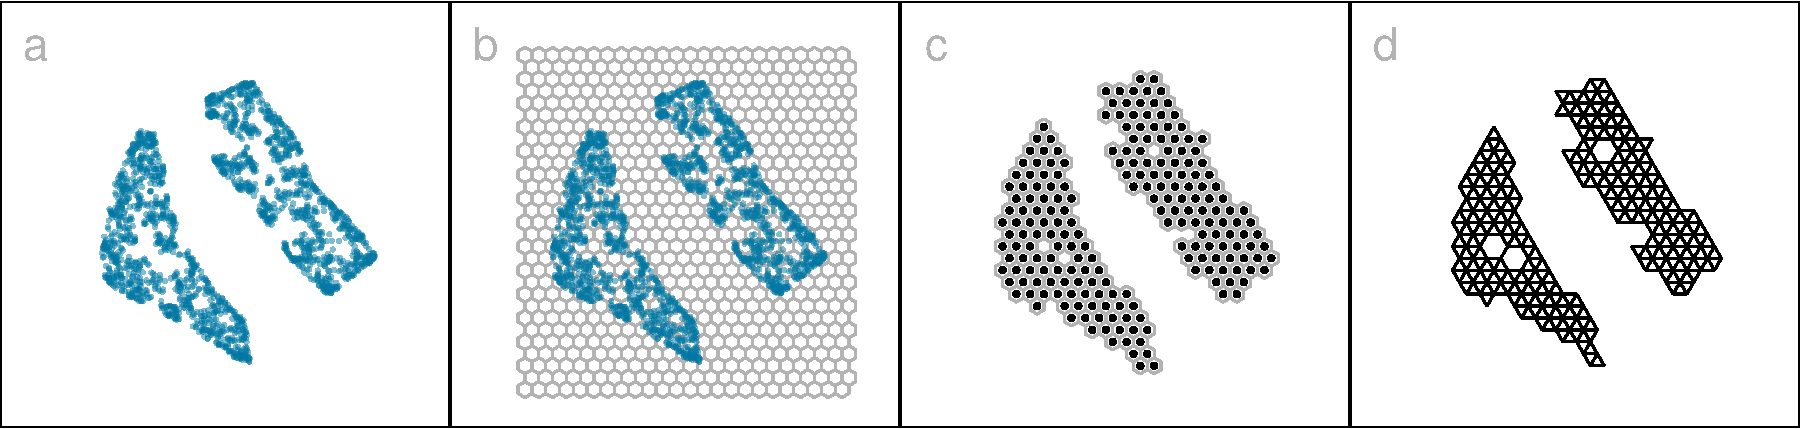
\includegraphics[width=1\linewidth,height=\textheight,keepaspectratio]{chapters/02-chap2_files/figure-pdf/fig-NLDR-two-curvy-1.pdf}

}

\caption{\label{fig-NLDR-two-curvy}Key steps for constructing the model
on the tSNE layout (\(k=2\)) of 2NC7: (a) data, (b) hexagon bins, (c)
bin centroids, and (d) triangulated centroids. The 2NC7 data is shown.}

\end{figure}%

\subsection{\texorpdfstring{Algorithm to represent the model in
\gD{}}{Algorithm to represent the model in }}\label{algorithm-to-represent-the-model-in}

\subsubsection{Scale the data}\label{scale-the-data}

Because we are working with distances between points, starting with data
having a standard scale, e.g.~{[}0, 1{]}, is recommended. The default
should take the aspect ratio produced by the NLDR
\((r_1, r_2, ..., r_k)\) into account. When \(k=2\), as in hexagon
binning, the default range is \([0, y_{i,\text{max}}], i=1,2\), where
\(y_{1,\text{max}}=1\) and \(y_{2,\text{max}} = r_2/r_1\)
(Figure~\ref{fig-NLDR-two-curvy}). If the NLDR aspect ratio is ignored
then set \(y_ {2,\text{max}} = 1.\)

\subsubsection{Hexagon grid
configuration}\label{hexagon-grid-configuration}

Although there are several implementations of hexagon binning
(\citeproc{ref-carr1987}{Carr et al. 1987}), and a published paper
(\citeproc{ref-dan2023}{Carr et al. 2023}), surprisingly, none has
sufficient detail or components that produce everything needed for this
project. So we described the process used here.
Figure~\ref{fig-hex-param} illustrates the notation used.

The \gD{} hexagon grid is defined by its bin centroids. Each hexagon,
\(H_h\) (\(h = 1, \dots, b\)) is uniquely described by centroid,
\(C_{h}^{(2)} = (c_{h1}, c_{h2})\). The number of bins in each direction
is denoted as \((b_1, b_2)\), with \(b = b_1 \times b_2\) being the
total number of bins. We expect the user to provide just \(b_1\) and we
calculate \(b_2\) using the NLDR ratio, to compute the grid.

To ensure that the grid covers the range of data values a buffer
parameter (\(q\)) is set as a proportion of the range. By default,
\(q=0.1\). The buffer should be extending a full hexagon width (\(a_1\))
and height (\(a_2\)) beyond the data, in all directions. The lower left
position where the grid starts is defined as \((s_1, s_2)\), and
corresponds to the centroid of the lowest left hexagon,
\(C_{1}^{(2)} = (c_{11}, c_{12})\). This must be smaller than the
minimum data value. Because it is one buffer unit, \(q\) below the
minimum data values, \(s_1 = -q\) and \(s_2 = -qr_2\).

The value for \(b_2\) is computed by fixing \(b_1\). Considering the
upper bound of the first NLDR component, \(a_1 > (1+2q)/(b_1 -1)\).
Similarly, for the second NLDR component,

\[
a_2 \geq \frac{r_2 + q(1 + r_2)}{(b_2 - 1)}.
\]

Since \(a_2 = \sqrt{3}a_1/2\) for regular hexagons,

\[
a_1 \geq \frac{2[r_2 + q(1 + r_2)]}{\sqrt{3}(b_2 - 1)}.
\]

This is a linear optimization problem. Therefore, the optimal solution
must occur on a vertex. Therefore,

\begin{equation}\phantomsection\label{eq-bin2}{
b_2 = \Big\lceil1 +\frac{2[r_2 + q(1 + r_2)](b_1 - 1)}{\sqrt{3}(1 + 2q)}\Big\rceil.
}\end{equation}

\begin{figure}[H]

\centering{

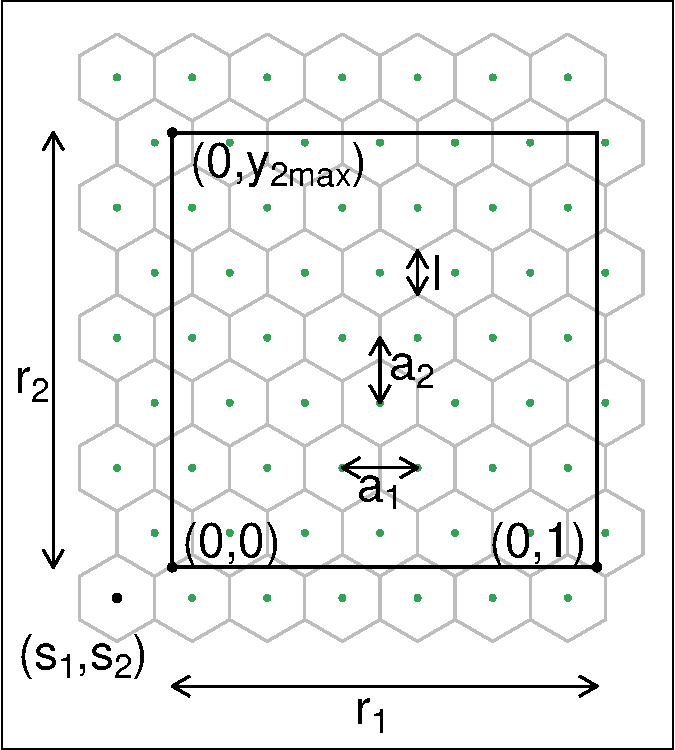
\includegraphics[width=0.3\linewidth,height=\textheight,keepaspectratio]{chapters/02-chap2_files/figure-pdf/fig-hex-param-1.pdf}

}

\caption{\label{fig-hex-param}The components of the hexagon grid
illustrating notation.}

\end{figure}%

\subsubsection{Binning the data}\label{binning-the-data}

Observations are grouped into bins based on their nearest centroid. This
produces a reduction in size of the data from \(n\) to \(m\), where
\(m\leq b\) (total number of bins). This can be defined using the
function
\(u: \mathbb{R}^{n\times 2} \rightarrow \mathbb{R}^{m\times 2}\), where
\[u(i) = \arg\min_{j = 1, \dots, b} \sqrt{(y_{i1} - C^{(2)}_{j1})^2 + (y_{i2} - C^{(2)}_{j2})^2},\]
maps observation \(i\) into \(H_h = \{i| u(i) = h\}\).

By default, the bin centroid is used for describing a hexagon (as done
in Figure~\ref{fig-NLDR-two-curvy} (c)), but any measure of center, such
as a mean or weighted mean of the points within each hexagon, could be
used. The bin centers, and the binned data, are the two important
components needed to render the model representation in high dimensions.

\subsubsection{Indicating neighborhood}\label{indicating-neighborhood}

Delaunay triangulation (\citeproc{ref-alb2024}{Gebhardt et al. 2024};
\citeproc{ref-lee1980}{Lee and Schachter 1980}) is used to connect
points so that edges indicate neighboring observations, in both the NLDR
layout (Figure~\ref{fig-NLDR-two-curvy} (d)) and the \pD{} model
representation. When the data has been binned the triangulation connects
centroids. The edges preserve the neighborhood information from the
\gD{} representation when the model is lifted into \pD{}.

\subsection{\texorpdfstring{Rendering the model in
\pD{}}{Rendering the model in }}\label{rendering-the-model-in}

The last step is to lift the \gD{} model into \pD{} by computing \pD{}
vectors that represent bin centroids. We use the \pD{} mean of the
points in a given hexagon, \(H_h\), denoted \(C_{h}^{(p)}\), to map the
centroid \(C_{h}^{(2)} = (c_{h1}, c_{h2})\) to a point in \pD{}. Let the
\(j^{th}\) component of the \pD{} mean be

\[C_{hj}^{(p)} = \frac{1}{n_h}\sum_{i =1}^{n_h} x_{hij}, ~~~h = 1, \dots, b;~ j=1, \dots, p; ~ n_h > 0.\]

\begin{figure}[H]

{\centering 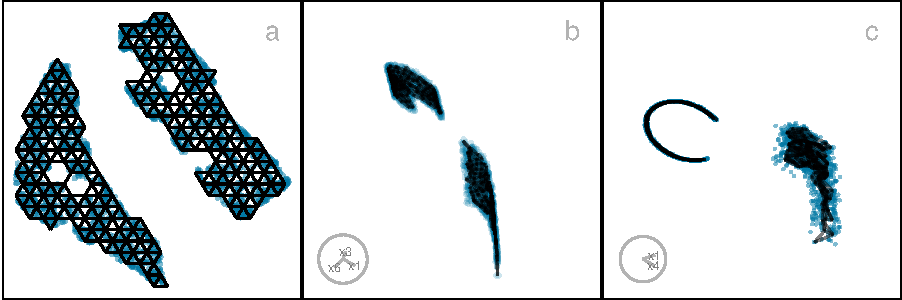
\includegraphics[width=1\linewidth,height=\textheight,keepaspectratio]{chapters/02-chap2_files/figure-pdf/best-fit-tsne-1.pdf}

}

\caption{Lifting the \gD{} fitted model into \pD{}. Two projections of
the \pD{} fitted model overlaying the data are shown in b, c.~The fit is
reasonably tight with the data in one cluster (top one in b), but
slightly less so in the other cluster probably because it is
\(3\text{-}D\). Notice also that, in the \gD{} layout the two clusters
have internal gaps which creates a model with some holes. This lacy
pattern happens regardless of the hyper-parameter choice, but this
doesn't severely impact the \pD{} model representation.}

\end{figure}%

\subsection{Measuring the fit}\label{sec-summary}

All NLDR methods internally optimize a quantity to produce a layout for
any particular hyper-parameter set. These are not always made available
in the model output, and may not be universally comparable between
hyper-parameter choices and methods.

Several common metrics are often used to assess the quality of any NLDR
layout, based on preservation of global and local structure of the data.
The \(RNX\) curve quantifies the neighborhood agreement between \pD{}
and \kD{} spaces, by computing the area under the curve (\(ARNX\))
across a range of neighborhood scales (\citeproc{ref-john2015}{Lee et
al. 2015}). A high value indicates better preservation of a balance of
global and local structure. Random Triplet Accuracy (RTA) and Centroid
Triplet Accuracy compare the order of \gD{} and \pD{} distances of
random triplets of points (\citeproc{ref-yingfan2021}{Wang et al.
2021}). High values indicate preservation of the geometry, suggesting
both local and global structure preservation. The Shepard diagram
(\citeproc{ref-shepard1962}{Shepard 1962}) and its associated Spearman
correlation (SC) (\citeproc{ref-spearman1961}{Spearman 1961}) between
\pD{} and \kD{} distances. High values indicate preservation of global
structure. The Global Score (GS) measures how well an embedding retains
the overall geometry of the data relative to a PCA baseline
(\citeproc{ref-amid2019}{\textbf{amid2019?}}). Higher values indicate
better preservation of global structure.

None of the above measures is particularly well-suited to assessing our
model fit, as we will show later. Thus, we need to different approach to
measuring model fit. Because the model here is similar to a confirmatory
factor analysis model (see a general explanation in Brown
(\citeproc{ref-brown2015}{2015})), \(\widehat{T} + \epsilon\), our
approach is similar to the ones used in this area. it is based on
``residuals'' computed as the difference between the fitted model and
observed values in \pD{}. Observations are associated with their bin
center, \(C_{h}^{(p)}\), which are also considered to be the
\emph{fitted values}. In factor analysis language, these fitted values
might also be denoted as \(\widehat{X}\). The error is computed by
taking the squared \pD{} Euclidean distance, of points from their bin
centroid, which we will call hexbin error (HBE):

\begin{equation}\phantomsection\label{eq-equation1}{ HBE = \sqrt{\frac{1}{n}\sum_{h = 1}^{m}\sum_{i = 1}^{n_h}\sum_{j = 1}^{p} (\mathbfit{x}_{hij} - C^{(p)}_{hj})^2}}\end{equation}

where \(n\) is the number of observations, \(m\) is the number of
non-empty bins, \(n_h\) is the number of observations in \(h^{th}\) bin,
\(p\) is the number of variables and \(\mathbfit{x}_{hij}\) is the
\(j^{th}\) dimensional data of \(i^{th}\) observation in \(h^{th}\)
hexagon. We can consider
\(e_{hi} = \sqrt{\sum_{j = 1}^{p} (\mathbfit{x}_{hij} - C^{(p)}_{hj})^2}\)
to be the residual for each observation.
Figure~\ref{fig-p-d-error-in-2d-two-curvy} shows plots of \(e\) as a
density (a), coloring the points in the NLDR layout (b) and the points
in a tour (c). It can be see that the biggest residuals are in one
cluster, which occurs due the intentional design that one cluster is
slightly \tD{} and perfectly captured by a \gD{} layout.

\begin{figure}[H]

\centering{

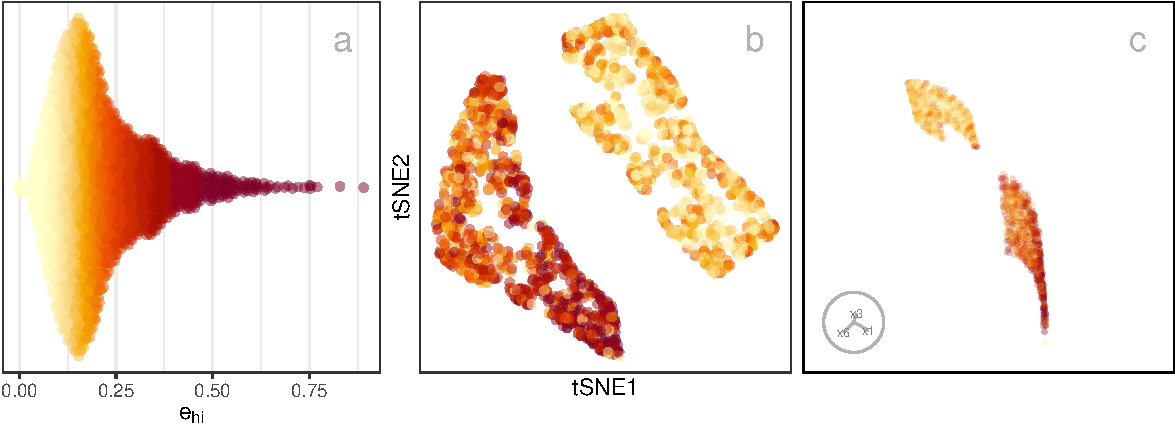
\includegraphics[width=1\linewidth,height=\textheight,keepaspectratio]{chapters/02-chap2_files/figure-pdf/fig-p-d-error-in-2d-two-curvy-1.pdf}

}

\caption{\label{fig-p-d-error-in-2d-two-curvy}Examining the distribution
of residuals in a jittered dotplot (a), \gD{} NLDR layout (b) and a tour
of \fD{} data space (c). Color indicates residual (\(e_{hi}\)), dark
color indicating high value. Most large residuals are distributed in one
cluster (bottom one in c) and most small residuals are distributed in
the other cluster.}

\end{figure}%

\subsection{\texorpdfstring{Prediction into
\gD{}}{Prediction into }}\label{prediction-into}

NLDR methods are primarily designed for visualization and exploration
rather than reconstruction, and do not explicitly provide out-of-sample
prediction. Of the five methods studied here, only UMAP provides a
\texttt{predict()} function for embedding new data points based on the
learned manifold (\citeproc{ref-tomasz2023}{Konopka 2023}). Several
other approaches, not used here, PCA, neural network autoencoders
(\citeproc{ref-hinton2006}{Hinton and Salakhutdinov 2006}) and
parametric tSNE (\citeproc{ref-van2009}{Maaten 2009}) support
prediction.

A benefit of our approach is that for any NLDR method, it provides a way
to predict the layout position of a new observation, \(x'\). The steps
are (1) determine the closest bin centroid in \pD{}, \(C^{(p)}_{h}\) and
(2) predict the embedding to be the bin centroid in \gD{},
\(C^{(2)}_{h}\).

\subsection{Tuning}\label{tuning}

The model fitting is based on these parameters:

\begin{itemize}
\tightlist
\item
  hexagon bin parameters

  \begin{itemize}
  \tightlist
  \item
    bottom left bin position \((s_1, \ s_2)\),
  \item
    the number of bins in the horizontal direction (\(b_1\)), which
    controls the number of bins the vertical direction (\(b_2\)), total
    number of bins (\(b\)), and total number of non-empty bins (\(m\)).
  \end{itemize}
\item
  low count bin removal using standardized bin counts
  (\(w_h = n_h/n, ~~h=1, \dots m\)).
\end{itemize}

Default values are provided for each of these, but deciding on the best
model fit is assisted by examining a range of values. The default number
of bins \(b=b_1\times b_2\) is computed based on the sample size, by
setting \(b_1=n^{1/3}\), consistent with the Diaconis-Freedman rule
(\citeproc{ref-freedman1981}{Freedman and Diaconis 1981}). The value of
\(b_2\) is determined analytically by \(b_1, q, r_2\)
(Equation~\ref{eq-bin2}). Values of \(b_1\) between \(2\) and
\(b_1 = \sqrt{n/r_2}\) are recommended, where the dependence on \(r_2\)
reflects the preservation of aspect ratio in the NLDR layout.

Figure~\ref{fig-bins-two-curvy} shows the hexbin grids for three choices
of \(b_1\). While the number of bins is the common parameter to modify,
bin start positions \((s_1, \ s_2)\) can be worth experimenting with
also because it can also change bin counts.

\begin{figure}[H]

\centering{

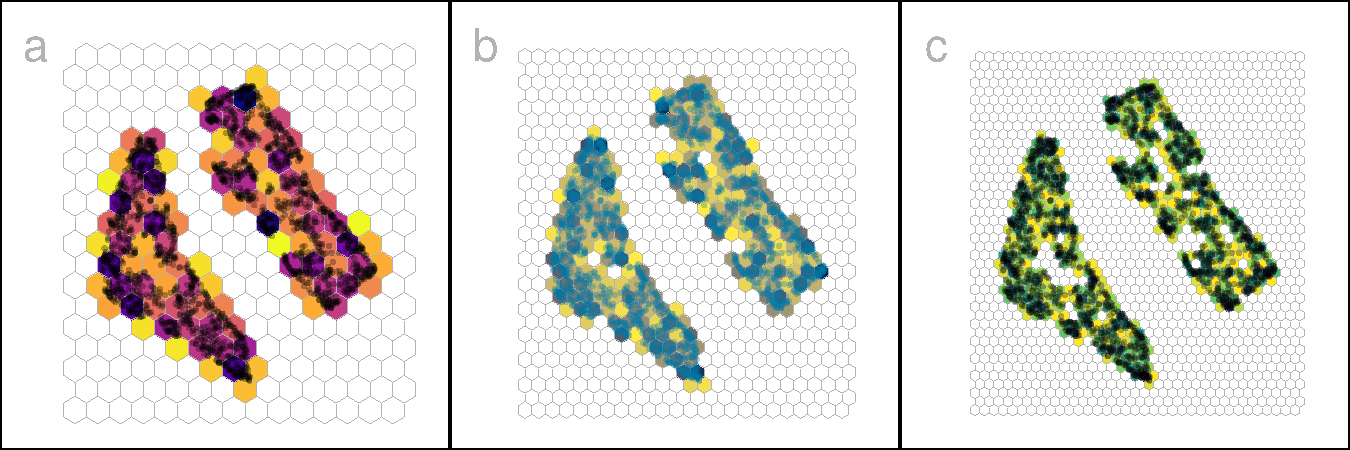
\includegraphics[width=1\linewidth,height=\textheight,keepaspectratio]{chapters/02-chap2_files/figure-pdf/fig-bins-two-curvy-1.pdf}

}

\caption{\label{fig-bins-two-curvy}Hexbin density plots of tSNE layout
of the 2NC7 data, using three different \(b_1\) specifications yielding
different \(b_2, b, m\): (a) \textbf{15}, 18, 270, 98, (b) \textbf{24},
29, 696, 209, and (c) \textbf{35}, 42, 1470, 386. Color indicates
standardized counts, dark indicating high count and light indicates low
count. At the smallest bin size, the data structure is discontinuous,
suggesting that there are too many bins.}

\end{figure}%

It is worthwhile to consider what are desirable aspects of a hexbin
result, that maps to summarizing the \pD{} fit well. The binning should
capture the underlying data distribution closely, with minimum number of
necessary bins. An ideal binning might be indicated by a more uniform
distribution of bin counts, or having few relatively empty bins. To help
with this assessment average bin count (\(\bar{n} = \sum{n_h}/m\)),
average standardized bin count (\(\bar{w} = \sum{w_h}/m\)) and
proportion of non-empty bins (\(m/b\)), are also computed.
Figure~\ref{fig-param-two-curvy} shows some choices of plots of these
quantities for a single NLDR layout, with three choices of \(a_1\)
indicated. Some expectations and reasoning for these plots is:

\begin{itemize}
\tightlist
\item
  HBE will increase as \(a_1\) increases, so good choices will be just
  before a big increase. In plot a, HBE changes fairly steadily so there
  is no easy choice to make.
\item
  HBE can also be examined against average standardized bin count or
  average bin count (plot b). This is similar to the comparison with
  \(a_1\) but to use when comparing different NLDR layouts. Different
  layouts might produce different density of points, which will not be
  captured well by a comparison of HBE vs \(a_1\).
\item
  The proportion of non-empty bins is interesting to examine across
  different binwidths (plot c). A good binning should have just the
  right amount of bins to neatly cover the shape of the data, and no
  more or less. As binwidth gets smaller, \(m/b\) should roughly get
  bigger.
\item
  Bins with a small number of observations might be removed to sharpen
  the wireframe model. This can have adverse effects, though - failing
  to extend the wireframe into sparse areas, or resulting in holes in
  the wireframe. Plot d shows the relationship between HBE (computed for
  all observations despite some bin removal) and the standardized bin
  count cutoff used to remove bins. For all three chosen bin widths a
  small number of bins can be removed without affecting HBE.
\end{itemize}

\begin{figure}[H]

\centering{

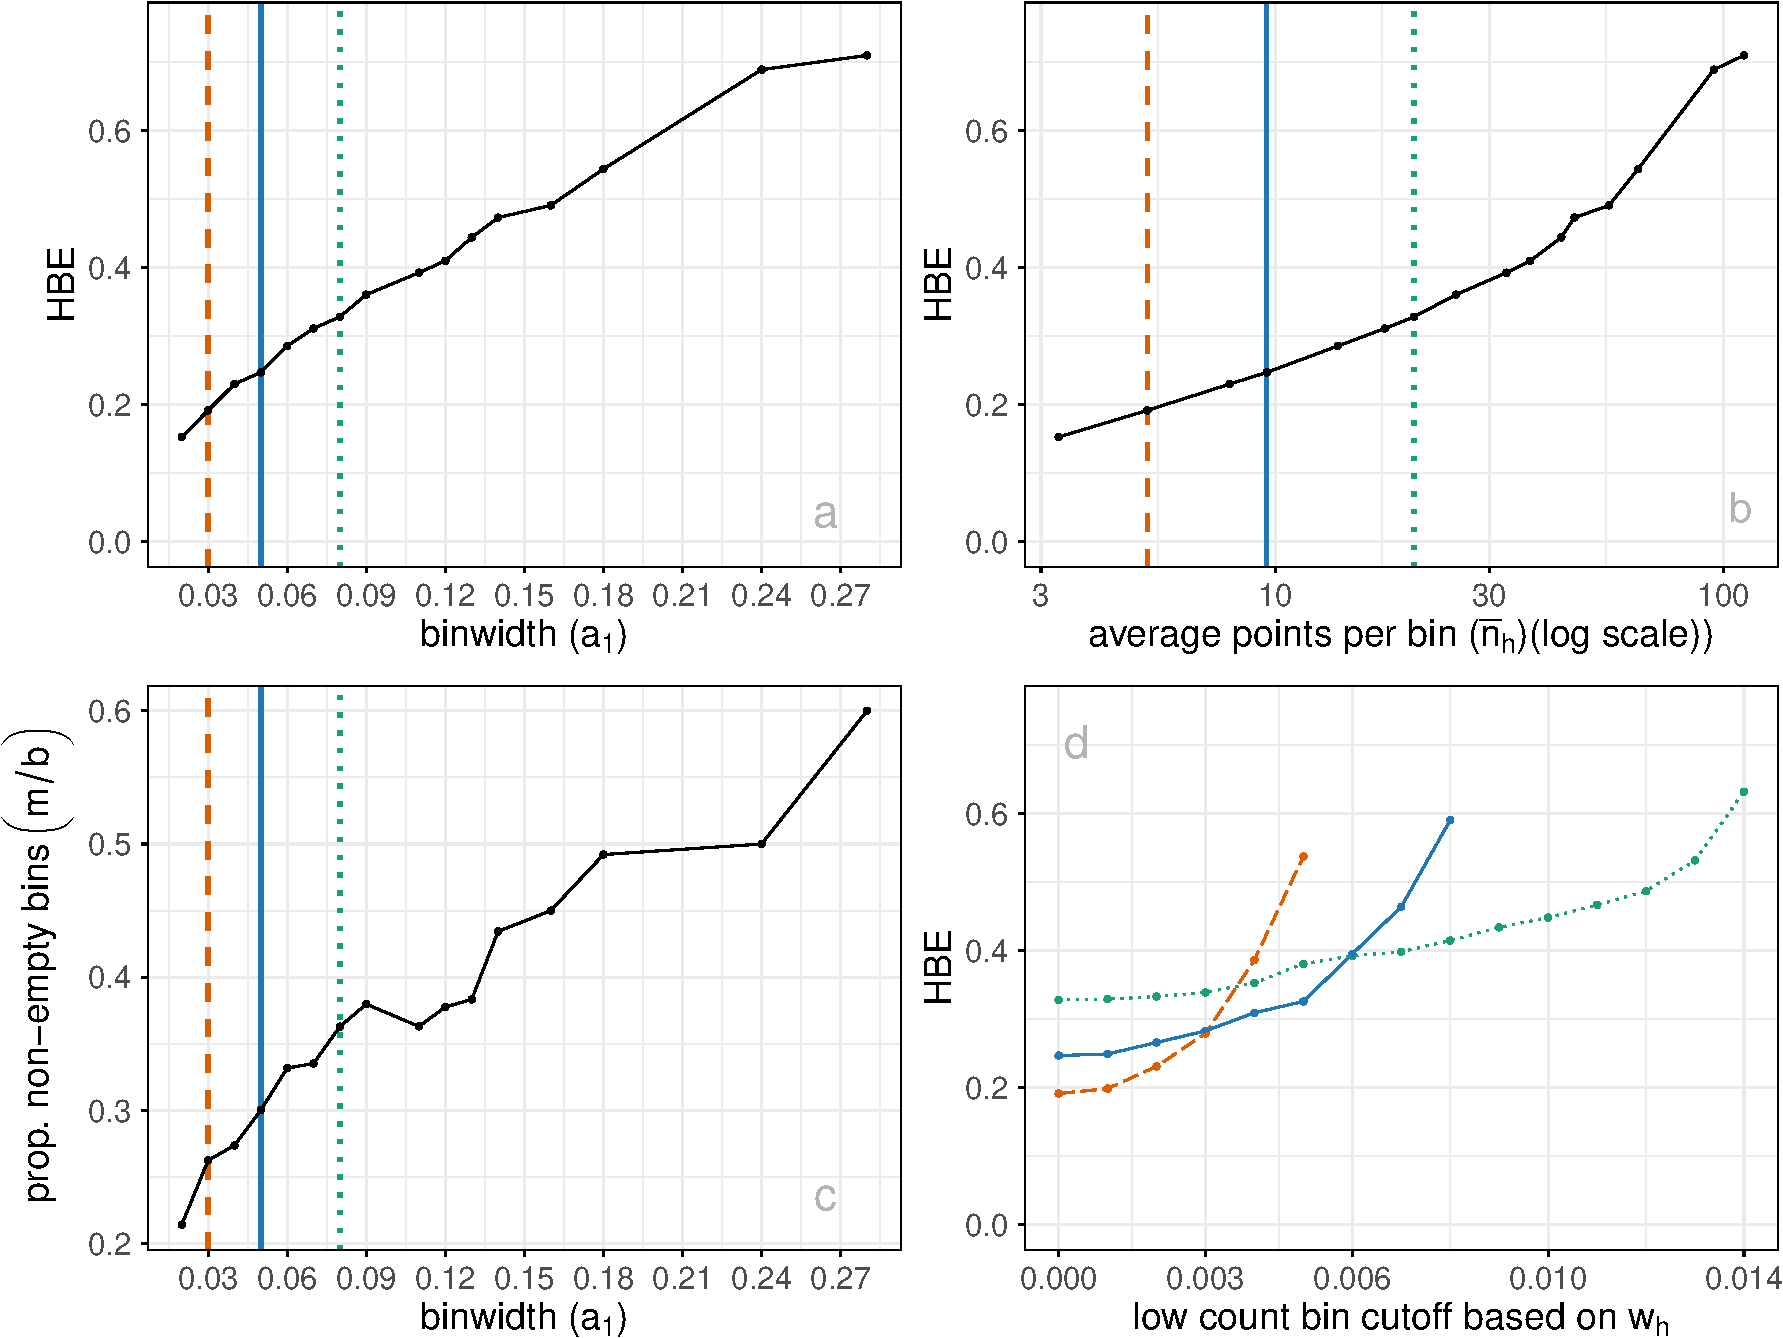
\includegraphics[width=1\linewidth,height=\textheight,keepaspectratio]{chapters/02-chap2_files/figure-pdf/fig-param-two-curvy-1.pdf}

}

\caption{\label{fig-param-two-curvy}Various plots to help tune the model
fit: (a) HBE vs \(a_1\), (b) HBE vs \(\bar{n}_h\), (c) proportion of
non-empty bins (\(m/b\)) vs \(a_1\), (d) HBE vs \(w_h\) cutoff used for
removing low count bins. Color indicates the three binwidths show in
Figure 6: \(0.03\) (orange dashed), \(0.05\) (blue solid), and \(0.08\)
(green dotted). The better model fit will have low HBE, but reasonably
sized bins that capture the data sufficiently. Proportion of non-empty
bins tends to increase with \(a_1\) (c). Removing a few low count bins
doesn't substantially change HBE, for all three binwidths (d).}

\end{figure}%

\subsection{Interactive graphics}\label{interactive-graphics}

Matching points in the \gD{} layout with their positions in \pD{} is
useful when tuning the fit. This can be used to examine the fitted model
in some subspaces in \pD{}, in particular in association with residual
plots.

The interactive \gD{} layout
(\citeproc{ref-chapman2020}{\textbf{chapman2020?}}) and the langevitour
(\citeproc{ref-harisson2024}{Harrison 2023}) view with the fitted model
overlaid can be linked using a browsable HTML widget
((\citeproc{ref-joe2025}{\textbf{joe2025?}}),
(\citeproc{ref-joe2024}{\textbf{joe2024?}})). A rectangular ``brush'' is
used to select points in one plot, which will highlight the
corresponding points in the other plot(s). Because the langevitour is
dynamic, brush events that become active will pause the animation, so
that a user can interrogate the current view. This approach will be
illustrated on the examples, to show how it can help to understand how
the NLDR has organised the observations, and learn where it does not do
well.

\section{\texorpdfstring{Choosing the best \gD{}
layout}{Choosing the best  layout}}\label{sec-bestfit}

Figure~\ref{fig-toy-rmse} illustrates the approach to compare the fits
for different representations and assess the strength of any fit. What
does it mean to be a best fit for this problem? Analysts use an NLDR
layout to display the structure present in high-dimensional data in a
convenient \gD{} display. It is a competitor to linear dimension
reduction that can better represent nonlinear associations such as
clusters. However, these methods can hallucinate, suggesting patterns
that don't exist, and grossly exaggerate other patterns. Having a layout
that best fits the high-dimensional structure is desirable but more
important is to identify bad representations so they can be avoided. The
goal is to help users decide on a the most useful and appropriate
low-dimensional representation of the high-dimensional data.

A particular pattern that we commonly see is that analysts tend to pick
layouts with clusters that have big separations between them. When you
examine their data in a tour, it is almost always that we see there are
no big separations, and actually often the suggested clusters are not
even present. While we don't expect that analysts include animated gifs
of tours in their papers, we should expect that any \gD{} representation
adequately indicates the clustering that is present, and honestly show
lack of separation or lack of clustering when it doesn't exist. It is
important for analysts to have tools to select the accurate
representation not the pretty but wrong representation.

To decide on a layout an analyst needs:

\begin{itemize}
\tightlist
\item
  a selection of NLDR representations made with a range of
  hyper-parameter choices and possibly different methods (tSNE, UMAP,
  \ldots).
\item
  a range of model fits made by varying bin size and low density bin
  removal.
\item
  calculated HBE for each layout, when it is transformed into the \pD{}
  space.
\item
  and the ability to examine the fit in the data space.
\end{itemize}

Comparing the HBE to obtain the best fit is appropriate if the same NLDR
method is used. However, because the HBE is computed on \pD{} data it
measures the fit between model and data so it can also be used to
compare the fit of different NLDR methods. A lower HBE indicates a
better NLDR representation.

\begin{figure}[H]

\centering{

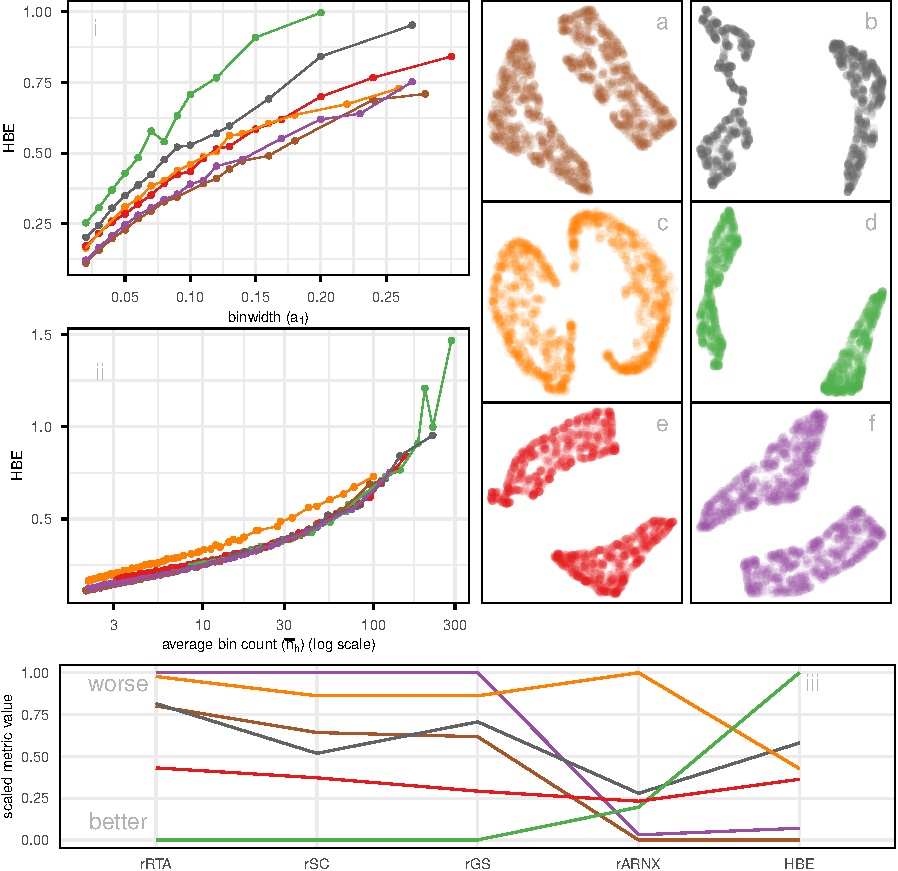
\includegraphics[width=1\linewidth,height=\textheight,keepaspectratio]{chapters/02-chap2_files/figure-pdf/fig-toy-rmse-1.pdf}

}

\caption{\label{fig-toy-rmse}Assessing which of the 6 NLDR layouts (a-f)
on the 2NC7 data is the better representation using HBE for varying
binwidth (\(a_1\)) and average bin count (\(\bar{n}_h\)). Color
represents NLDR layout. Layout d is universally poor. Layouts a, b, e
that show two close clusters are universally suboptimal. Layout b with
little separation performs well at tiny binwidth (where most points are
in their own bin) and poorly as binwidth increases. Layout e has small
separation with oddly shaped clusters. Layout a is the best choice.
Comparison of scaled evaluation metrics (rRTA, rSC, rGS, rARNX, and HBE
using \(a_1=0.05\)) for the six NLDR layouts computed on the 2NC7 data
using a parallel coordinate plot. Color of the line indicates NLDR
layout. RTA, SC, GS, and ARNX is reversed so that lower is best.}

\end{figure}%

Figure~\ref{fig-toy-rmse} compares the metrics ARNX, RTA, SC, GS, along
with HBE computed on \(a_1=0.05\) for the six layouts shown in
Figure~\ref{fig-toy-rmse}. This is a parallel coordinate plot where the
y-axis shows a normalized score to ensure the metrics are on the same
scale. Each line corresponds to one layout. The metric ARNX has been
reversed so that it aligns with HBE - the lower the value the better the
layout.

There is some agreement between the metrics. All, except ARNX agree that
layout d is worst. All agree that layout f is best or very close to
best. Layout a is best according to HBE and ARNX but considered to be
much less optimal by RTA, SC and GS. Layout c is considered favorably by
RTA, SC and GS but to be very poor by ARNX. This illustrates how
difficult it is to use the numerical metrics alone to decide on the best
layout.

Ironically, RTA, GS and SC should be interpreted as ``the higher the
better'', but here they agree with HBE and ARNX when interpreted in
reverse! The problem with SC is that correlation is not a good measure
in the presence of clusters - the further the clusters are apart in the
layout produces a Shepard plot with two clusters of distances which will
produce a high correlation value. Similar reasoning would explain why
RTA and GS behave similarly: they put too much emphasis on the global
structure. Thus, for the 2NC7 data further apart clusters score better,
overly emphasizing that there are two clusters, even though this
separation is not accurately reflecting the difference in \pD{}.

When the metrics disagree is causes confusion for the analyst, and thus
provides a temptation to choose the nicest looking layout (very
separated clusters), even though it may be a hallucination. Because HBE
is accompanied with a representation of the layout in \pD{} to compare
with the observed data, it can help to add more clarity in making
decisions. Figure~\ref{fig-fit-tsne-phate} shows the fitted models for
layouts a (rated high by HBE and ARNX) and c (rated poorly). These are
\gD{} projectiosn from the tour, with black indicating the fitted model
overlaid on the blue points of the data. The reason for the poor fit is
that the PHATE layout (c) twists extremely along the 2- and \tD{}
manifolds where the data lies. We have learned that all the NLDR methods
tend to have twists in the fit in \pD{} but this is extreme. This is
likely why layout c has poor metrics relative to the other layouts, and
it suggests that it does not adequately capture the local structure in
the 2NC7 data.

\begin{figure}

\centering{

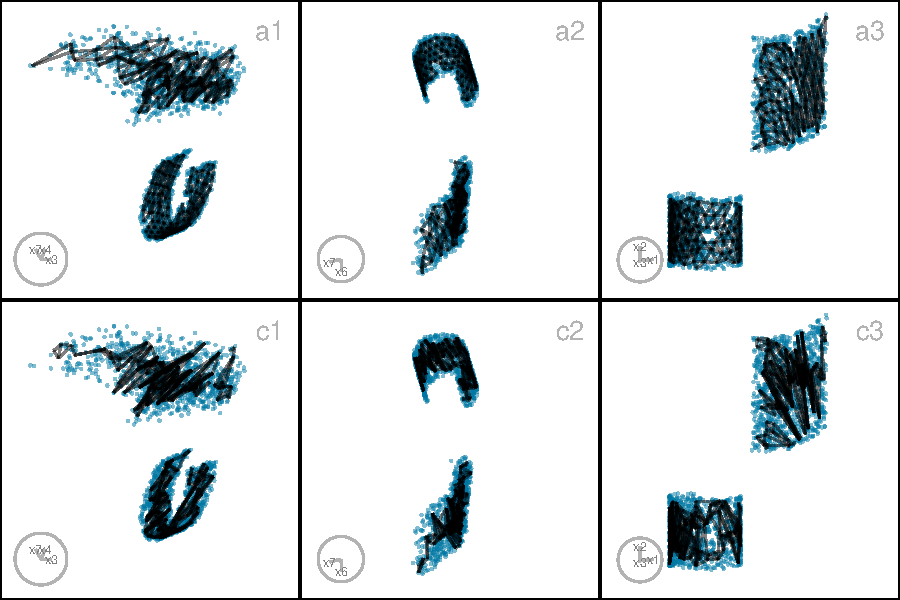
\includegraphics[width=1\linewidth,height=\textheight,keepaspectratio]{chapters/02-chap2_files/figure-pdf/fig-fit-tsne-phate-1.pdf}

}

\caption{\label{fig-fit-tsne-phate}Three \(2\text{-}D\) projections from
a tour showing the fitted models (black lines) for layouts a (top row)
and c (bottom row) of the 2NC7 data (blue points). Layout c, which was
poorly rated by ARNX and HBE covers less of the width of the data than
a. The triangular gridding is less visible in c than a, and actually
corresponds to extreme twisting.}

\end{figure}%

\section{Applications}\label{sec-applications}

To illustrate the approach we use two examples: PBMC3k data (single cell
gene expression) where an NLDR layout is used to represent cluster
structure present in the \pD{} data, and MNIST hand-written digits where
NLDR is used to represent essentially a low-dimensional nonlinear
manifold in \pD{}.

\subsection{PBMC3k}\label{sec-pbmc}

This is a benchmark single-cell RNA-Seq data set collected on Human
Peripheral Blood Mononuclear Cells (PBMC3k) as used in Genomics
(\citeproc{ref-pbmc2019}{2016}). Single-cell data measures the gene
expression of individual cells in a sample of tissue (see for example,
Haque et al. (\citeproc{ref-haque2017}{2017})). This type of data is
used to obtain an understanding of cellular level behavior and
heterogeneity in their activity. Clustering of single-cell data is used
to identify groups of cells with similar expression profiles. NLDR is
often used to summarize the cluster structure. Usually, NLDR does not
use the cluster labels to compute the layout, but uses color to
represent the cluster labels when it is plotted.

In this data there are \(2622\) single cells and \(1000\) gene
expressions (variables). Following the same pre-processing as Chen et
al. (\citeproc{ref-chen2024}{2024}), different NLDR techniques were
performed on the first nine principal components.
Figure~\ref{fig-NLDR-variety} shows this data using a variety of
methods, and different hyper-parameters. You can see that the result is
wildly different depending on the choices. Layout a is a reproduction of
the layout that was published in Chen et al.
(\citeproc{ref-chen2024}{2024}). This layout suggests that the data has
three very well separated clusters, each with an odd shape. The question
is whether this accurately represents the cluster structure in the data,
or whether they should have chosen b or c or d or e or f or g or h. This
is what our new method can help with -- to decide which is the more
accurate \gD{} representation of the cluster structure in the \pD{}
data.

Figure~\ref{fig-pbmc-rmse} shows HBE across a range of binwidths
(\(a_1\)) for each of the layouts in Figure~\ref{fig-NLDR-variety}. The
layouts were generated using tSNE and UMAP with various hyper-parameter
settings, while PHATE, PaCMAP, and TriMAP were applied using their
default settings. Lines are color coded to match the color of the
layouts shown on the right. Lower HBE indicates the better fit. Using a
range of binwidths shows how the model changes, with possibly the best
model being one that is universally low HBE across all binwidths. It can
be seen that layout f is sub-optimal with universally higher HBE. Layout
a, the published one, is better but it is not as good as layouts b, d,
or e. With some imagination layout d perhaps shows three barely
distinguishable clusters. Layout e shows three, possibly four, clusters
that are more separated. The choice reduces from eight to these two.
Layout d has slightly better HBE when the \(a_1\) is small, but layout e
beats it at larger values. Thus we could argue that layout e is the most
accurate representation of the cluster structure, of these eight.

To further assess the choices, we need to look at the model in the data
space, by using a tour to show the wireframe model overlaid on the data
in the \(9\text{-}D\) space (Figure~\ref{fig-model-pbmc-author-proj}).
Here we compare the published layout (a) versus what we argue is the
best layout (e). The top row (a1, a2, a3) correspond to the published
layout and the bottom row (e1, e2, e3) correspond to the optimal choice
according to our procedure. The middle and right plots show two
projections. The primary difference between the two models is that the
model of layout e does not fill out to the extent of the data but
concentrates in the center of each point cloud. Both suggest that three
clusters is a reasonable interpretation of the structure, but layout e
more accurately reflects the separation between them, which is small.

\begin{figure}[H]

\centering{

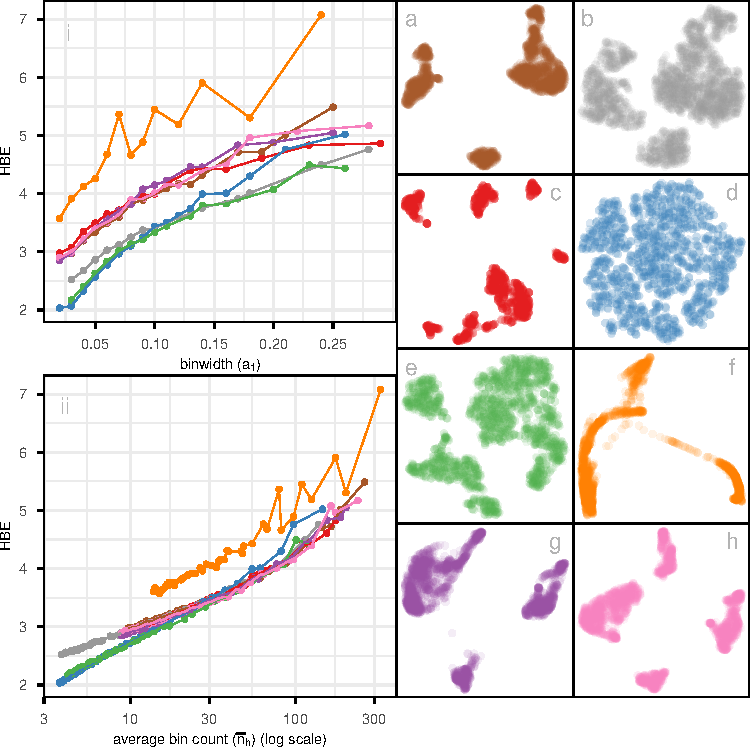
\includegraphics[width=1\linewidth,height=\textheight,keepaspectratio]{chapters/02-chap2_files/figure-pdf/fig-pbmc-rmse-1.pdf}

}

\caption{\label{fig-pbmc-rmse}Assessing which of the 8 NLDR layouts on
the PBMC3k data (shown in Figure~\ref{fig-NLDR-variety}) is the better
representation using HBE for varying binwidth (\(a_1\)). Color used for
the lines and points in the left plot and in the scatterplots represents
NLDR layout (a-h). Layout f is universally poor. Layouts a, c, g, h that
show large separations between clusters are universally suboptimal.
Layout d with little separation performs well at tiny binwidth (where
most points are in their own bin) and poorly as binwidth increases. The
choice of best is between layouts b and e, that have small separations
between oddly shaped clusters. Layout e is chosen as the best.}

\end{figure}%

\begin{figure}[H]

\centering{

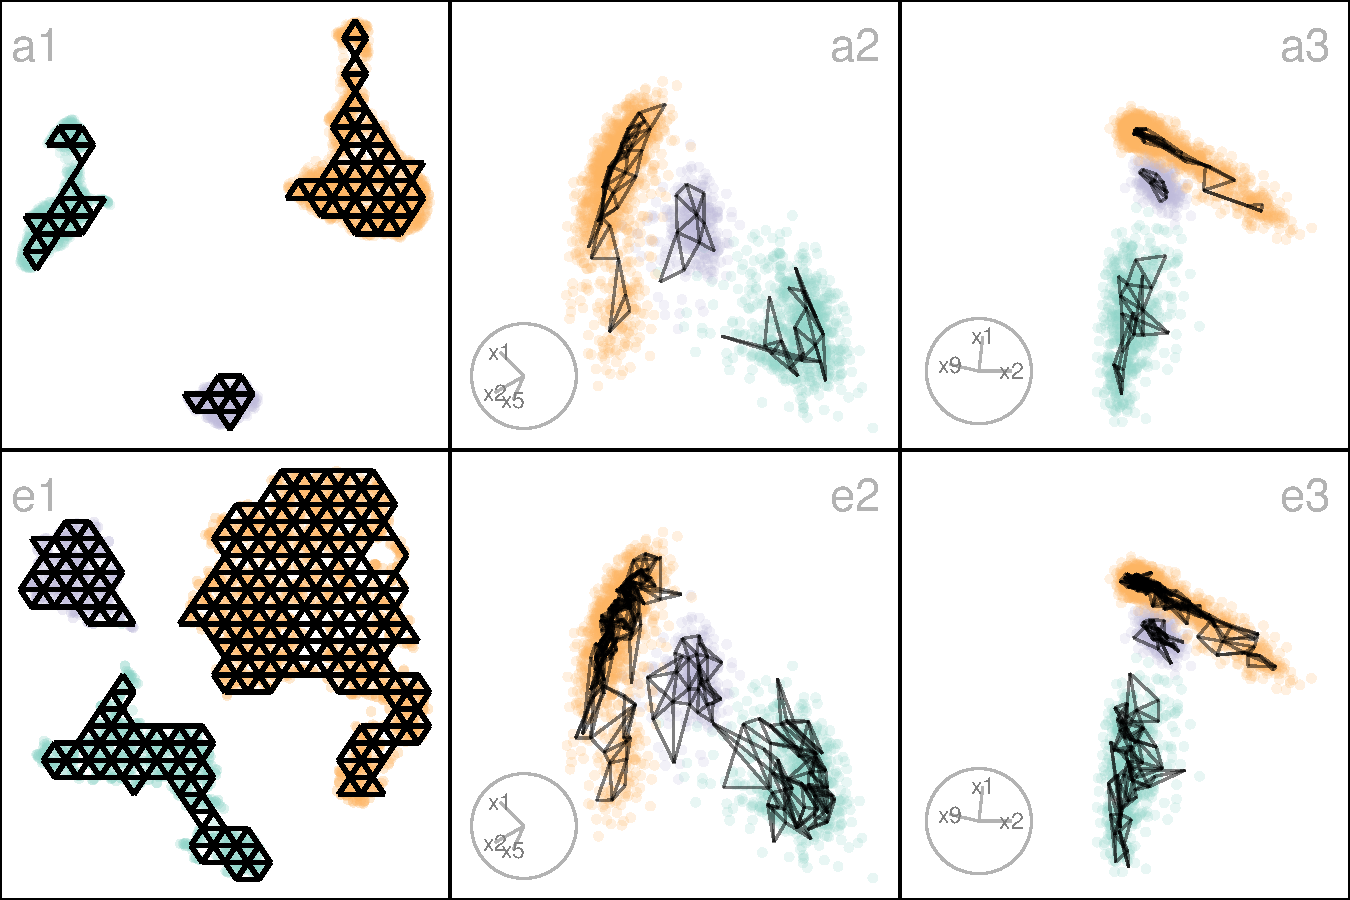
\includegraphics[width=0.9\linewidth,height=\textheight,keepaspectratio]{chapters/02-chap2_files/figure-pdf/fig-model-pbmc-author-proj-1.pdf}

}

\caption{\label{fig-model-pbmc-author-proj}Compare the published \gD{}
layout (a) made with UMAP and the \gD{} layout selected by HBE plot (e)
made by tSNE. The two plots on the right show projections from a tour,
with the models overlaid. The published layout a suggested three very
separated clusters, but this is not present in the data. While there may
be three clusters they are not well-separated. The difference in model
fit also indicates this: the published layout a does not spread out
fully into the point cloud like the model generated from layout e. This
supports the choice that layout e is the better representation of the
data, because it does not exaggerate separation between clusters.}

\end{figure}%

\subsection{MNIST hand-written digits}\label{sec-mnist}

The digit ``1'' of the MNIST dataset (\citeproc{ref-lecun1998}{LeCun et
al. 1998}) consists of \(7877\) grayscale images of handwritten ``1''s.
Each image is \(28 \times 28\) pixels which corresponds to \(784\)
variables. The first \(10\) principal components, explaining \(83\%\) of
the total variation, are used. This data essentially lies on a nonlinear
manifold in the high dimensions, defined by the shapes that ``1''s make
when sketched. We expect that the best layout captures this type of
structure and does not exhibit distinct clusters.

\begin{figure}[H]

\centering{

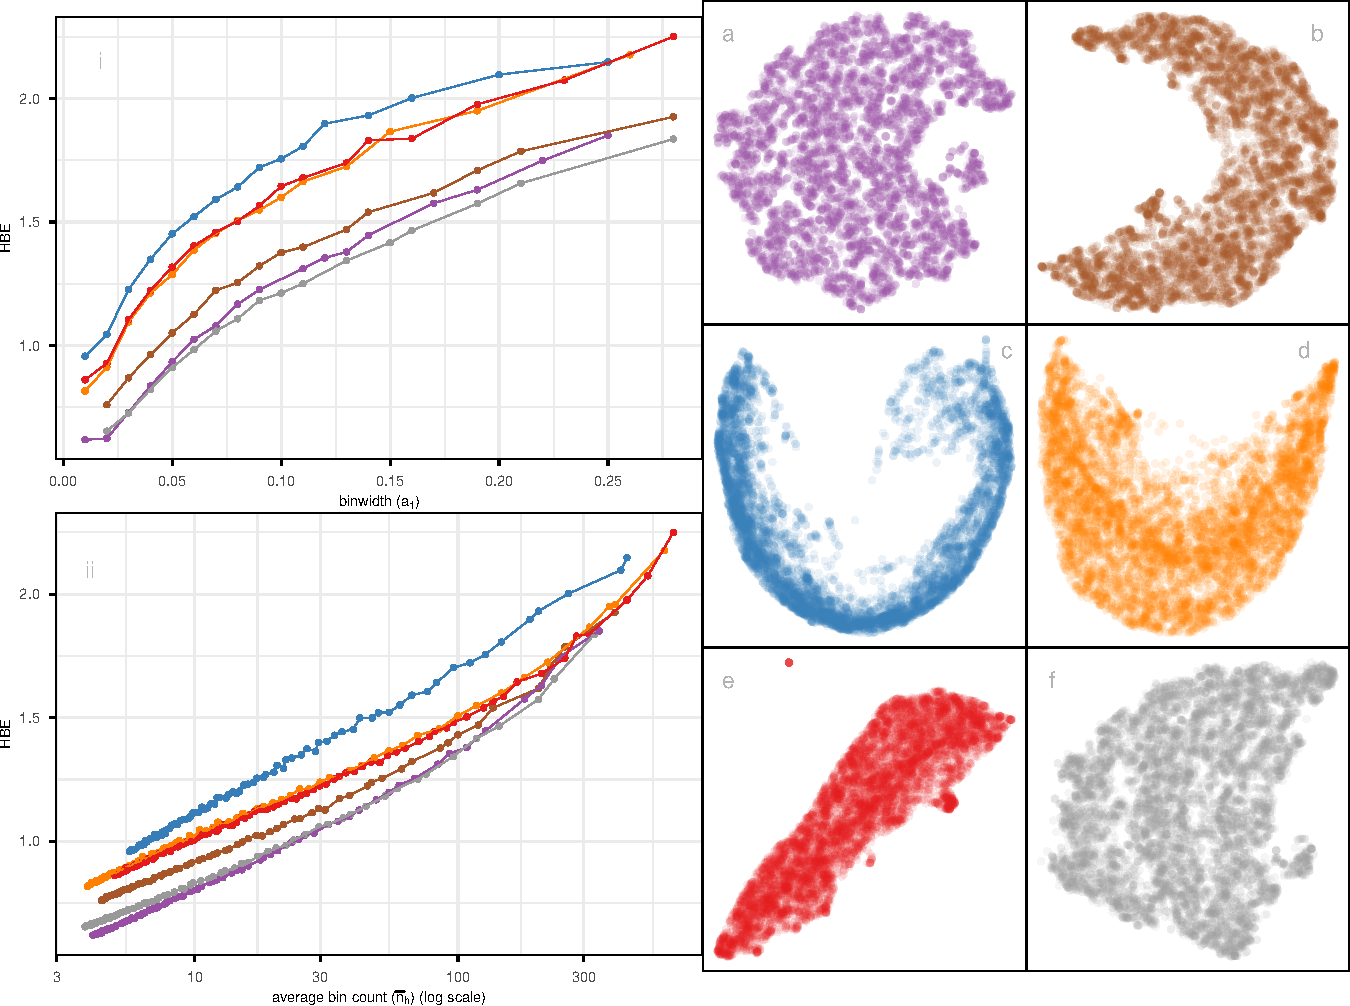
\includegraphics[width=0.92\linewidth,height=\textheight,keepaspectratio]{chapters/02-chap2_files/figure-pdf/fig-mnist-rmse-1.pdf}

}

\caption{\label{fig-mnist-rmse}Assessing which of the 6 NLDR layouts of
the MNIST digit 1 data is the better representation using HBE for
varying binwidth (\(a_1\)). Colour is used for the lines and points in
the left plot to match the scatterplots of the NLDR layouts (a-f).
Layout c is universally poor. Layouts a, f that show a big cluster and a
small circular cluster are universally optimal. Layout a performs well
at tiny binwidth (where most points are in their own bin) and not as
well as f with larger binwidth, thus layout f is the best choice.}

\end{figure}%

Figure~\ref{fig-mnist-rmse} compares the fit of six layouts computed
using UMAP (b), PHATE (c), TriMAP (d), PaCMAP (e) with default
hyper-parameter setting and two tSNE runs, one with default
hyper-parameter setting (a) and the other changing perplexity to \(89\)
(f). The layouts are reasonably similar in that they all have the
observations in a single blob. Some (b, c) have a more curved shape than
others. Layout e is the most different having a linear shape, and a
single very large outlier. Both a and f have a small clump of points
perhaps slightly disconnected from the other points, in the lower to
middle right.

The layout plots are colored to match the lines in the HBE vs binwidth
(\(a_1\)) plot. Layouts a, b and f fit the data better than c, d, e, and
layout f appears to be the best fit. Figure~\ref{fig-clust-mnist} shows
this model in the data space in two projections from a tour. The data is
curved in the \(10\text{-}D\) space, and the fitted model captures this
curve. The small clump of points in the \gD{} layout is highlighted in
both displays. These are almost all inside the curve of the bulk of
points and are sparsely located. The fact that they are packed together
in the \gD{} layout is likely due to the handling of density differences
by the NLDR.

An interesting aside is that the rather strange layout e, which has what
looks like a single point far from the remaining observations is
actually similar to this one. That point is actually a clump of points
corresponding to some of the diffuse points interior to the curve of the
bulk of points. This is easy to see using the linked brushing tool.

The next step is to investigate the \gD{} layout to understand what
information is learned from this representation.
Figure~\ref{fig-model-error-mnist} summarizes this investigation. Plot a
shows the layout with points colored by their residual value - darker
color indicates larger residual and poor fit. The plots b, c, d, e show
samples of hand-written digits taken from inside the colored boxes.
Going from top to bottom around the curve shape we can see that the
``1''s are drawn with from right slant to a left slant. The ``1''s in d
(black box) tend to have the extra up stroke but are quite varied in
appearance. The ``1''s shown in the plots labelled e correspond to
points with big residuals. They can be seen to be more strangely drawn
than the others. Overall, this \gD{} layout shows a useful way to
summarize the variation in way ``1''s are drawn.

\begin{figure}[H]

\centering{

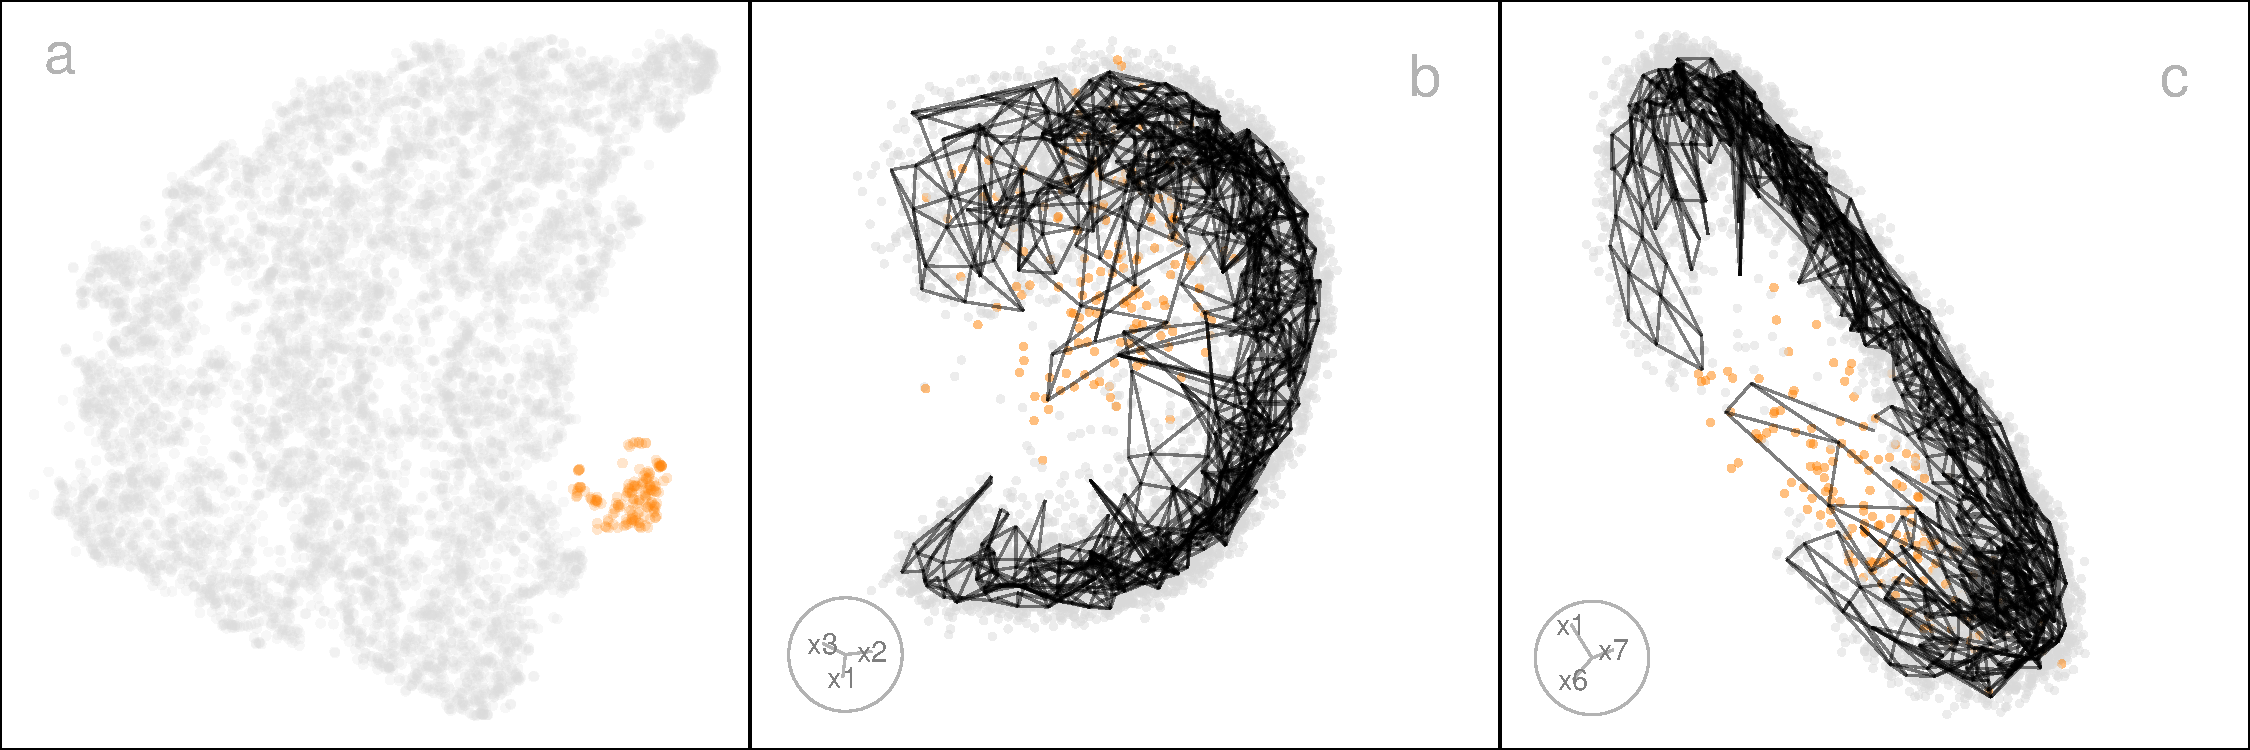
\includegraphics[width=1\linewidth,height=\textheight,keepaspectratio]{chapters/02-chap2_files/figure-pdf/fig-clust-mnist-1.pdf}

}

\caption{\label{fig-clust-mnist}Summary from exploring tSNE layout of
the MNIST digit 1 data (a in Figure 12) using linked brushing. There is
a big nonlinear cluster (grey) and a small cluster (orange) located very
close to the one corner of the big cluster in \gD{} (a). The MNIST digit
1 data has a nonlinear structure in \(10\text{-}D\). Two \gD{}
projections from a tour on \(10\text{-}D\) reveal that the small orange
cluster is actually a diffuse set of points wrapped within the grey
cluster, which is C-shaped in the high dimensions.}

\end{figure}%

\begin{figure}[H]

\centering{

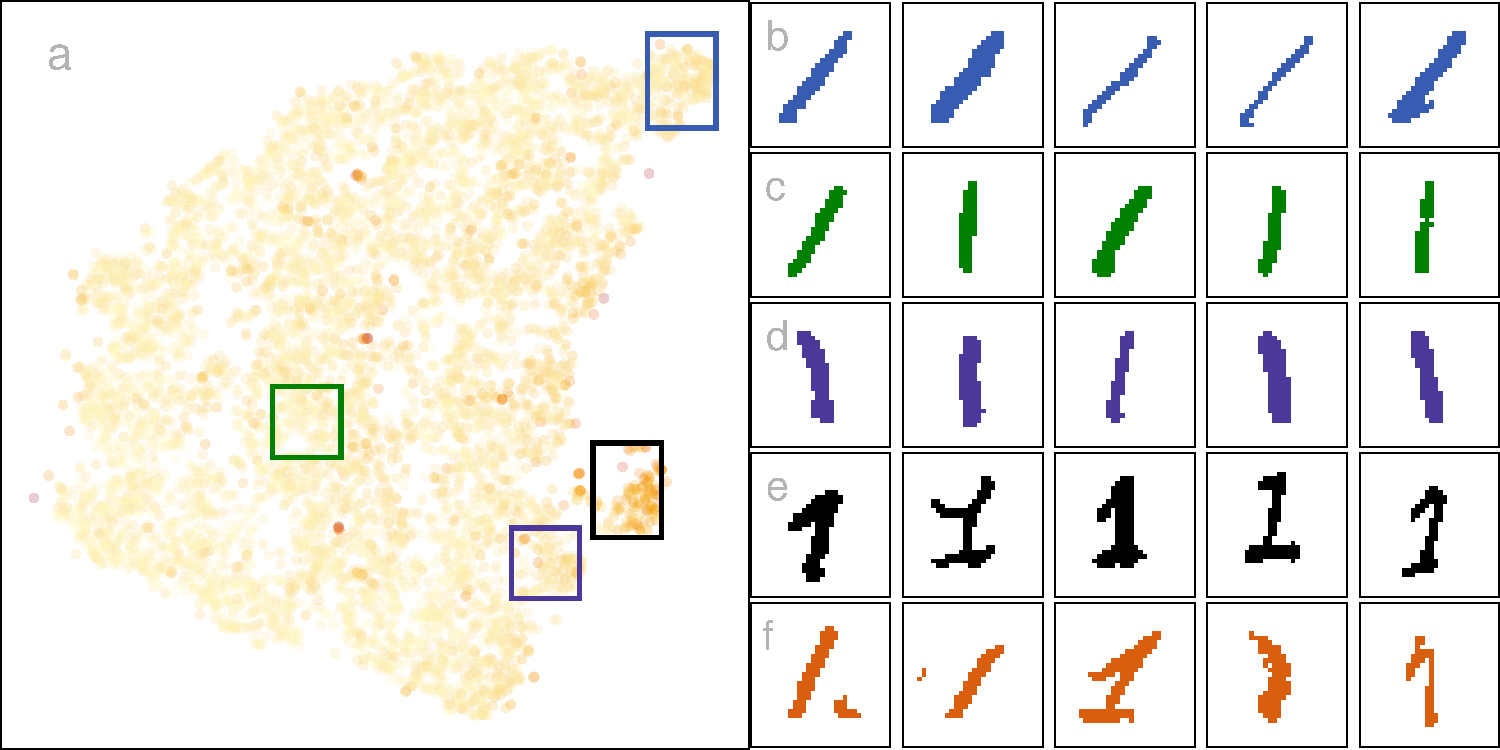
\includegraphics[width=1\linewidth,height=\textheight,keepaspectratio]{chapters/02-chap2_files/figure-pdf/fig-model-error-mnist-1.pdf}

}

\caption{\label{fig-model-error-mnist}Summary of the layout structure,
and large errors, relative to the MNIST digit 1 shape: (a) layout
colored by residual value, and at right (b-e) are images of samples of
observations taken at locations around the layout, showing similarity in
how the 1's were drawn. Set (f) are images corresponding to large
residuals in the big cluster (darker orange in plot a). Along the big
cluster, the angle of digit 1 changes (b-d). The small cluster has
larger residuals, and the images show that these tend to be European
style with a flag at the top, and a base at the bottom. The set in (f)
show various poorly written digits.}

\end{figure}%

\section{Discussion}\label{sec-discussion}

We have developed an approach to help assess and compare NLDR layouts,
generated by different methods and hyper-parameter choice(s). It depends
on conceptualizing the \gD{} layout as a model, allowing for the
creation of a wireframe representation of the model that can be lifted
into \pD{}. The fit is assessed by viewing the model in the data space,
computing residuals and HBE. Different layouts can be compared using the
HBE, providing quantitative and objective metrics to decide on the most
suitable NLDR layout to represent the \pD{} data. Global and local
preservation of structure is assessed by examining the HBE across a
range of binwidths. It also provides a way to predict the values of new
\pD{} observations in the \gD{}, which could be useful for implementing
uncertainty checks such as using training and testing samples.

Two examples illustrating usage are provided: the PBMC3k data where the
NLDR is summarizing clustering in \pD{} and hand-written digits
illustrating how NLDR represents an intrinsically lower dimensional
nonlinear manifold. We examined a typical published usage of UMAP with
the PBMC3k dataset (Chen, 2024). As is typical of UMAP layout with
default settings, the separation between clusters is grossly
exaggerated. The layout even suggests separation where there is none.
Our approach provides a way to objectively choose the layout and
hopefully avoids the use of misleading layouts in the future. In the
hand-written digits we illustrate how our model fit statistics show that
a flat disc layout is superior to the curved shaped layouts, and how to
identify oddly written ``1''s using the residuals of the fitted model.

This work can be applied with existing metrics for evaluating NLDR
layout, such as ARNX, RTA, sc, and RGS. It provides an additional
evaluation metric, and allows any layout to viewed the in the \pD{} data
space. This latter aspect can help to disentangle conflicting
suggestions by the different metrics. Additional exploration of metrics
to summarize the fit could be a new direction for the work. The
difficulty is capturing nonlinear fits, for which Euclidean distance can
be sub-optimal. We have used a very simple approach based on clustering
methods, Euclidean distances to nearest centroid, which can approximate
nonlinear patterns. Other cluster metrics would be natural choices to
explore.

This work has also revealed some interesting curiosities about NLDR
procedures. They almost all twist to fit data in \pD{}. Sometimes the
fitted model appears as a ``pancake'' in some data where clusters are
regularly shaped and high-dimensional, for some methods but not others,
which is odd. One can imagine that if algorithms are initiated using
principal components then some ordering of points along the major axes
might generate this pattern. Alternatively, if local distances dominate
the algorithm then is might be possible to see this pattern with
well-separated regular clusters. We also demonstrated that there is a
tendency for NLDR algorithms to be confused by different density in the
data space, and some patterns in the layout are due to density
differences rather than nonlinear associations between variables.

Most NLDR methods only provide a \gD{} but if a \kD{} (\(k>2\)) layout
is provided the approach developed here could be extended. Binning into
cubes could be done in \(3\text{-}D\) or higher, relatively easily, and
used as a the basis for a wireframe of the fitted model. Barber et al.
(\citeproc{ref-barber1996}{1996}) (and the associated software Laurent
(\citeproc{ref-stephane2023}{2023})) has an algorithm for a convex hull
in \pD{} which serves as an inspiration. A simpler approach using
\(k\)-means clustering to provide centroids could also be possible, but
the complication would be to determine how to connect the centroids into
an appropriate wireframe.

The new methodology is accompanied by an R package called quollr, so
that it is readily usable and broadly accessible. The package has
methods to fit the model, compute diagnostics and also visualize the
results, with interactivity. We have primarily used the langevitour
software (\citeproc{ref-harisson2024}{Harrison 2023}) to view the model
in the data space, but other tour software such as tourr
(\citeproc{ref-wickham2011}{Wickham et al. 2011}) and detourr
(\citeproc{ref-hart2022}{Hart and Wang 2022}) could be also used.

\section{Supplementary Materials}\label{sec-supplementary}

All the materials to reproduce the paper can be found at
\url{https://github.com/JayaniLakshika/paper-nldr-vis-algorithm}. The
Appendix includes many more details.

The R package \texttt{quollr}, available on CRAN and at
\url{https://jayanilakshika.github.io/quollr/}, provides software
accompaying this paper to fit the wireframe model representation,
compute diagnostics, visualize the model in the data with langevitour
and link multiple plots interactively.

\section{Acknowledgments}\label{acknowledgments}

These \texttt{R} packages were used for the work: \texttt{tidyverse}
(\citeproc{ref-hadley2019}{Wickham et al. 2019}), \texttt{Rtsne}
(\citeproc{ref-jesse2015}{Krijthe 2015}), \texttt{umap}
(\citeproc{ref-tomasz2023}{Konopka 2023}), \texttt{patchwork}
(\citeproc{ref-thomas2024}{Pedersen 2024}), \texttt{colorspace}
(\citeproc{ref-achim2020}{Zeileis et al. 2020}), \texttt{langevitour}
(\citeproc{ref-harisson2024}{Harrison 2023}), \texttt{conflicted}
(\citeproc{ref-hadley2023}{Wickham 2023}), \texttt{reticulate}
(\citeproc{ref-kevin2024}{Ushey et al. 2024}), \texttt{kableExtra}
(\citeproc{ref-hao2024}{Zhu 2024}). These \texttt{python} packages were
used for the work: \texttt{trimap}
(\citeproc{ref-amid2019}{\textbf{amid2019?}}) and \texttt{pacmap}
(\citeproc{ref-yingfan2021}{Wang et al. 2021}). The article was created
with \texttt{R} packages \texttt{quarto}
(\citeproc{ref-jjallaire2024}{Allaire and Dervieux 2024}).

\bookmarksetup{startatroot}

\chapter{\texorpdfstring{quollr: An R Package for Visualizing
\(2\text{-}D\) Models from Non-linear Dimension Reductions in High
Dimensional
Space}{quollr: An R Package for Visualizing 2\textbackslash text\{-\}D Models from Non-linear Dimension Reductions in High Dimensional Space}}\label{sec-third-paper}

\section{Introduction}\label{introduction-1}

Non-linear dimension reduction (NLDR) techniques, such as t-distributed
stochastic neighbor embedding (tSNE) (\citeproc{ref-laurens2008}{Maaten
and Hinton 2008}), uniform manifold approximation and projection (UMAP)
(\citeproc{ref-leland2018}{McInnes et al. 2018}), potential of
heat-diffusion for affinity-based trajectory embedding (PHATE) algorithm
(\citeproc{ref-moon2019}{Moon et al. 2019}), large-scale dimensionality
reduction Using triplets (TriMAP)
(\citeproc{ref-amid2019}{\textbf{amid2019?}}), and pairwise controlled
manifold approximation (PaCMAP) (\citeproc{ref-yingfan2021}{Wang et al.
2021}), can create hugely different representations depending on the
selected method and hyper-parameter choices. It is difficult to
determine whether any of these representations are accurate, which one
is the best, or whether they have missed important structures.

This paper presents the R package, \texttt{quollr}, which is useful for
understanding how NLDR warps high-dimensional space and fits the data.
Starting with an NLDR layout, our approach is to create a
\twoD wireframe model representation, that can be lifted and displayed
in the high-dimensional (\pD{}) space (Figure @ref(fig:overview)).

\begin{figure}[H]

{\centering 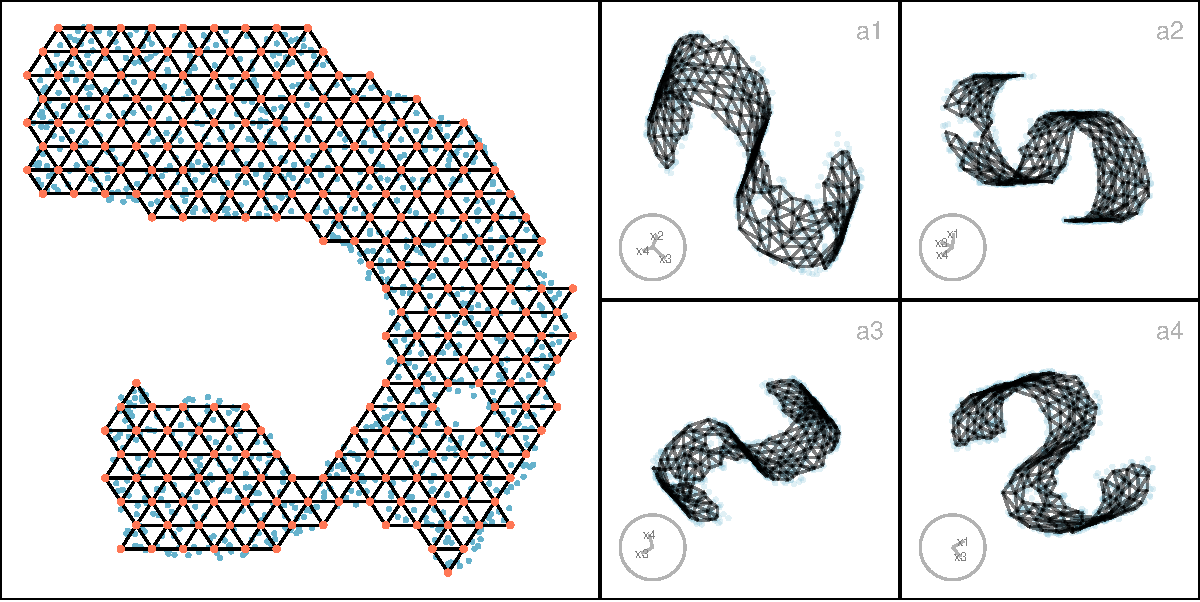
\includegraphics[width=1\linewidth,height=\textheight,keepaspectratio]{chapters/03-chap3_files/figure-pdf/overview-1.pdf}

}

\caption{Wireframe model representation of the NLDR layout, lifted and
displayed in high-dimensional space. The left panel shows the NLDR
layout with a triangular mesh overlay, forming the wireframe structure.
This mesh can be lifted into higher dimensions and projected to examine
how the geometric structure of the data is preserved. Panels (a1--a4)
display different \twoD projections of the lifted wireframe, where the
underlying curved sheet structure of the data is more clearly visible.
The triangulated mesh highlights how local neighborhoods in the layout
correspond to relationships in the high-dimensional space, enabling
diagnostics of distortion and preservation across dimensions.}

\end{figure}%

The paper is organized as follows. The next section introduces the
implementation of the \texttt{quollr} package on CRAN, including a
demonstration of the package's key functions and visualization
capabilities. In the application section, we illustrate the algorithm's
functionality for studying a clustering data structure. Finally, we
conclude the paper with a brief summary and discuss potential
opportunities for using our algorithm.

\section{Implementation}\label{implementation}

The implementation of \texttt{quollr} is designed to be efficient, and
easy to extend. The package is organized into a series of logical
components that reflect the main stages of the workflow: data
preprocessing, model fitting, low-density bin removal, prediction,
visualization, and interactive exploration (Figure @ref(fig:workflow)).
This package structure makes the code easier to maintain and allows new
features to be added without changing the existing functionality.

\begin{figure}[H]

{\centering 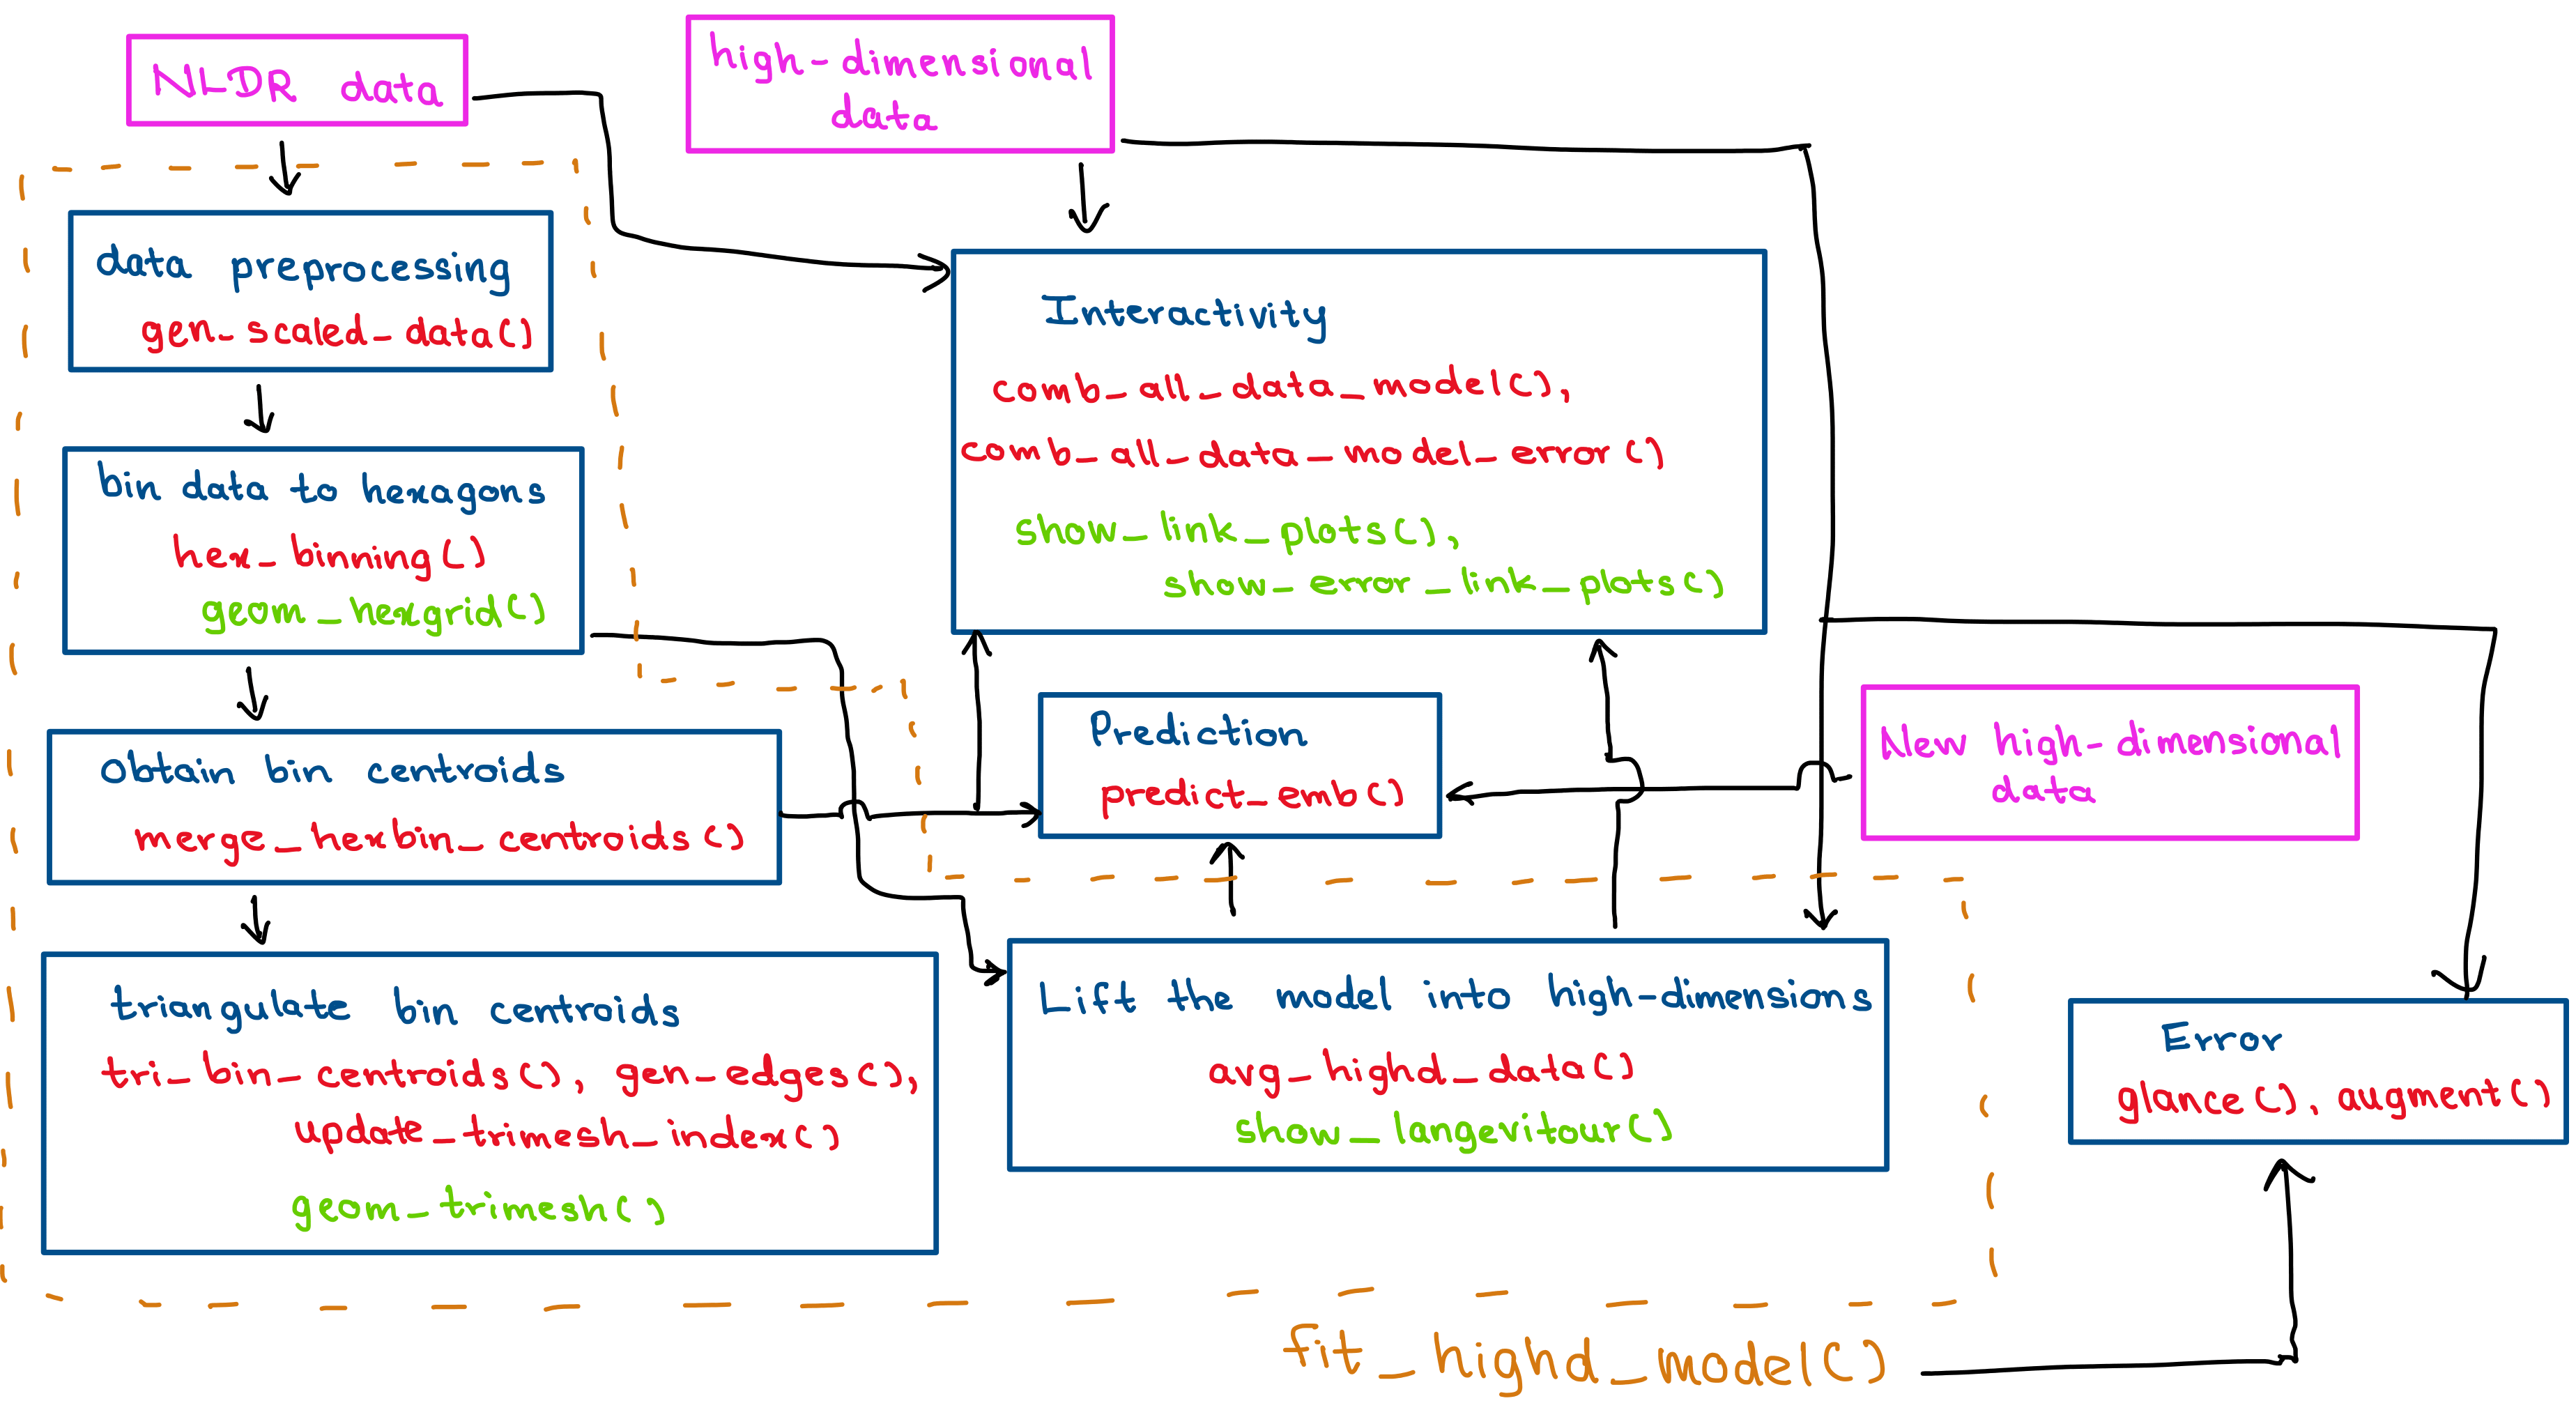
\includegraphics[width=1\linewidth,height=\textheight,keepaspectratio]{chapters/../figures/quollr/quollr_workflow.png}

}

\caption{Overview of the \texttt{quollr} workflow and software
architecture. The process begins with NLDR and \(p\text{-}D\) data
inputs, followed by data preprocessing and hexagonal binning. Centroids
are computed and triangulated to form the \(2\text{-}D\) mesh, which is
then lifted into the \(p\text{-}D\) space. Predictions and error
computations are performed on new data, while interactive functions
enable dynamic linking between the \(p\text{-}D\) and \(2\text{-}D\)
representations.}

\end{figure}%

\subsection{Software architecture}\label{software-architecture}

The package is organized into seven core modules corresponding to stages
of the analysis workflow: preprocessing, \twoD model construction,
lifting into \pD, prediction, error computation, visualization, and
interactivity. Each module performs a distinct task and communicates
through data objects.

\begin{enumerate}
\def\labelenumi{\arabic{enumi}.}
\item
  Data preprocessing: The function \texttt{gen\_scaled\_data()}
  standardizes the embedding data, manage variable naming, and ensure
  consistent identifiers across high-dimensional and embedded datasets.
\item
  Construct \twoD model: A series of functions \texttt{hex\_binning()},
  \texttt{merge\_hexbin\_centroids()}, \texttt{tri\_bin\_centroids()},
  \texttt{gen\_edges()}, and \texttt{update\_trimesh\_index()} generate
  the hexagonal grid, compute bin centroids, and connect the triangular
  mesh that defines local neighborhoods in the \twoD space.
\item
  Lift the model into \pD: The function \texttt{avg\_highd\_data()}
  computes the average of the high-dimensional variables for each bin,
  linking the \twoD representation back to the original data space.
\item
  Prediction: The function \texttt{predict\_emb()} estimates the
  embedding of new high-dimensional observations based on the fitted
  model.
\item
  Error computation: The \texttt{glance()} and \texttt{augment()}
  function summarizes model performance by comparing the predicted and
  original embeddings.
\item
  Visualization: Functions such as \texttt{geom\_hexgrid()},
  \texttt{geom\_trimesh()}, and \texttt{show\_langevitour()} provide
  tools for exploring the fitted models through static and dynamic
  visualizations.
\item
  Interactivity: The functions \texttt{comb\_all\_data\_model()} and
  \texttt{show\_link\_plots()} generate interactive linked
  visualizations that connect the \twoD NLDR layout, the corresponding
  tour view, and the fitted model. Similarly,
  \texttt{comb\_all\_data\_model\_error()} and
  \texttt{show\_error\_link\_plots()} integrate the error distribution
  with the \twoD embedding and dynamic high-dimensional view, enabling
  interactivity across multiple visual components.
\end{enumerate}

Each module is internally independent but connected through data objects
(see next section). This modular design simplifies maintenance and
allows developers to extend individual components such as substituting
different binning approaches, extracting centroids, or visualization
tools without altering the overall workflow.

\subsection{Data objects}\label{data-objects}

The internal data objects follow the tidy data principle: each variable
is stored in a column, each observation in a row, and each type of
information in its own table. This structure makes the package easy to
use with the \texttt{tidyverse} and other R visualization tools.

\subsubsection{Input objects}\label{input-objects}

\begin{itemize}
\item
  \texttt{highd\_data}: a tibble containing the original
  high-dimensional observations with a unique identifier (\texttt{ID})
  and variable columns prefixed with \texttt{"x"} (e.g., \texttt{x1},
  \texttt{x2}, \ldots).
\item
  \texttt{nldr\_data}: a tibble containing two-dimensional embeddings,
  labeled as \texttt{emb1} and \texttt{emb2}, matched to the same
  \texttt{ID}s.
\end{itemize}

\subsubsection{Generated objects}\label{generated-objects}

\begin{itemize}
\item
  \texttt{scaled\_nldr\_obj}: the output of
  \texttt{gen\_scaled\_data()}, which rescales the embedding to the
  range \([0, 1] \times [0, y_{2,\text{max}}]\), where
  \(y_{2,\text{max}} = r_2 / r_1\) is the ratio of the embedding ranges.
  It includes the scaled coordinates (\texttt{scaled\_nldr}) and the
  original limits (\texttt{lim1}, \texttt{lim2}).
\item
  \texttt{hex\_bin\_obj}: the object created by \texttt{hex\_binning()},
  which defines the structure of the two-dimensional hexagonal grid used
  in modeling. It includes the grid spacing (\texttt{a1}, \texttt{a2}),
  the number of bins along each axis, the centroids of all hexagons,
  polygon coordinates for plotting, and the mapping of each data point
  to its assigned hexagon.
\item
  \texttt{highd\_vis\_model}: the main model object returned by
  \texttt{fit\_highd\_model()}. It stores all components of the fitted
  visualization model, including the scaled NLDR data
  (\texttt{nldr\_scaled\_obj}), the hexagonal bin structure
  (\texttt{hb\_obj}), the averaged \pD summaries for each bin
  (\texttt{model\_highd}), the corresponding \twoD bin centroids
  (\texttt{model\_2d}), and the triangulated mesh connecting neighboring
  bins (\texttt{trimesh\_data}).
\end{itemize}

\subsection{Computational efficiency and
optimization}\label{computational-efficiency-and-optimization}

Several core computations within \texttt{quollr} are optimized using
compiled C++ code via the \texttt{Rcpp} and \texttt{RcppArmadillo}
packages. While the user interacts with high-level R functions,
performance-critical steps such as nearest-neighbor searches
(\texttt{compute\_highd\_dist()}), error metrics
(\texttt{compute\_errors()}), \twoD distance calculations
(\texttt{calc\_2d\_dist\_cpp()}), and generation of hexagon coordinates
(\texttt{gen\_hex\_coord\_cpp()}) are handled internally in C++. This
design provides significant speedups when analyzing large datasets while
maintaining a user-friendly R interface. These C++ functions are not
exported but are bundled within the package and fully accessible for
inspection in the source code.

\section{Usage}\label{usage}

The package is available on CRAN, and the development version is
available at https://jayanilakshika.github.io/quollr/.

Our algorithm includes the following steps: (1) scaling the NLDR data,
(2) computing configurations of a hexagon grid, (3) binning the data,
(4) obtaining the centroids of each bin, (5) indicating neighboring bins
with line segments that connect the centroids, and (6) lifting the model
into high dimensions (Figure @ref(fig:algo-steps)). A detailed
description of the algorithm can be found in
(\citeproc{ref-gamage2025c}{\textbf{gamage2025c?}}).

\begin{figure}[H]

{\centering 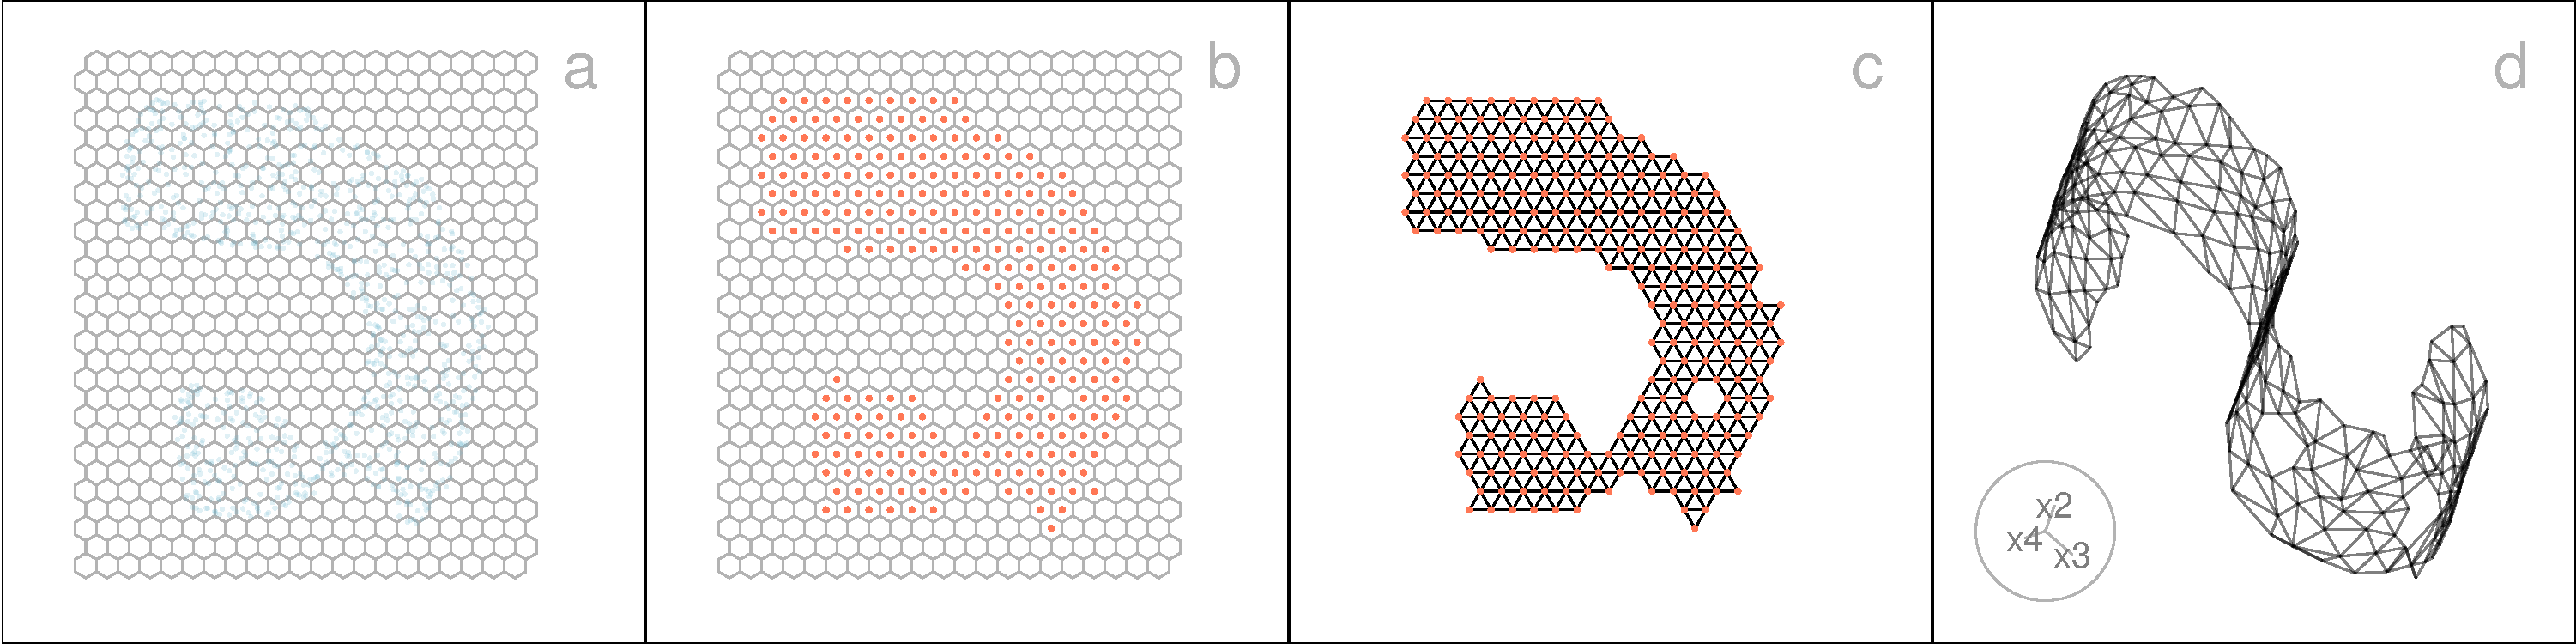
\includegraphics[width=1\linewidth,height=\textheight,keepaspectratio]{chapters/03-chap3_files/figure-pdf/algo-steps-1.pdf}

}

\caption{Key steps for constructing the model on the UMAP layout: (a)
hexagon bins, (b) bin centroids, (c) triangulated centroids, and (d)
lifting the model into high dimensions. The \texttt{Scurve} data is
shown.}

\end{figure}%

The following demonstration of the package's functionality assumes
\texttt{quollr} has been loaded. To begin the workflow, users need two
inputs: the high-dimensional dataset and the corresponding nonlinear
dimensionality reduction (NLDR) layout. The high-dimensional data must
contain a unique \texttt{ID} column, with data columns prefixed by the
letter \texttt{"x"} (e.g., \texttt{x1}, \texttt{x2}, etc.). The NLDR
dataset should include embedding coordinates labeled as \texttt{emb1}
and \texttt{emb2}, ensuring one-to-one correspondence with the
high-dimensional data through the shared \texttt{ID}.

To illustrate the workflow, we use the built-in example dataset
\texttt{scurve}, a \(7\text{-}D\) simulated dataset consisting of
\(1000\) observations. The first three variables define a \(3\text{-}D\)
S-shaped manifold, while the remaining four variables introduce
low-magnitude uniform noise, yielding a structured yet noisy
high-dimensional dataset.

\begin{Shaded}
\begin{Highlighting}[]
\FunctionTok{data}\NormalTok{(}\StringTok{"scurve"}\NormalTok{)}
\end{Highlighting}
\end{Shaded}

For this example, we use the UMAP layout, which is produced using
\texttt{n\_neighbors\ =} \(46\) and \texttt{min\_dist\ =} \(0.9\).

\begin{Shaded}
\begin{Highlighting}[]
\FunctionTok{library}\NormalTok{(umap)}
\FunctionTok{library}\NormalTok{(dplyr)}

\NormalTok{scurve\_umap }\OtherTok{\textless{}{-}} \FunctionTok{umap}\NormalTok{(}
\NormalTok{  scurve }\SpecialCharTok{|\textgreater{}} \FunctionTok{select}\NormalTok{(}\SpecialCharTok{{-}}\NormalTok{ID),}
  \AttributeTok{config =} \FunctionTok{modifyList}\NormalTok{(umap.defaults, }\FunctionTok{list}\NormalTok{(}
    \AttributeTok{n\_neighbors =} \DecValTok{46}\NormalTok{,}
    \AttributeTok{n\_components =} \DecValTok{2}\NormalTok{,}
    \AttributeTok{min\_dist =} \FloatTok{0.9}
\NormalTok{  ))}
\NormalTok{)}\SpecialCharTok{$}\NormalTok{layout }\SpecialCharTok{|\textgreater{}}
  \FunctionTok{as\_tibble}\NormalTok{(}\AttributeTok{.name\_repair =} \SpecialCharTok{\textasciitilde{}} \FunctionTok{paste0}\NormalTok{(}\StringTok{"emb"}\NormalTok{, }\DecValTok{1}\SpecialCharTok{:}\DecValTok{2}\NormalTok{)) }\SpecialCharTok{|\textgreater{}}
  \FunctionTok{mutate}\NormalTok{(}\AttributeTok{ID =}\NormalTok{ scurve}\SpecialCharTok{$}\NormalTok{ID)}
\end{Highlighting}
\end{Shaded}

\subsection{Main function}\label{main-function}

The mains steps for the algorithm can be executed by the main function
\texttt{fit\_highd\_model()}, or can be run separately for more
flexibility.

This function requires several parameters: the high-dimensional data
(\texttt{highd\_data}), the emdedding data (\texttt{nldr\_data}), the
number of bins along the x-axis (\texttt{b1}), the buffer amount as a
proportion of data (\texttt{q}), and benchmark value to extract high
density hexagons (\texttt{hd\_thresh}). The function returns an object
of class \texttt{highd\_vis\_model} containing the scaled NLDR object
(\texttt{nldr\_scaled\_obj}) with three elements: the first is the
scaled NLDR data (\texttt{scaled\_nldr}), and the second and third are
the limits of the original NLDR data (\texttt{lim1} and \texttt{lim2});
the hexagonal object (\texttt{hb\_obj}), the fitted model in both
\twoD (\texttt{model\_2d}), and \pD (\texttt{model\_highd}), and
triangular mesh (\texttt{trimesh\_data}).

\begin{Shaded}
\begin{Highlighting}[]
\FunctionTok{fit\_highd\_model}\NormalTok{(}
  \AttributeTok{highd\_data =}\NormalTok{ scurve, }
  \AttributeTok{nldr\_data =}\NormalTok{ scurve\_umap, }
  \AttributeTok{b1 =} \DecValTok{21}\NormalTok{, }
  \AttributeTok{q =} \FloatTok{0.1}\NormalTok{, }
  \AttributeTok{hd\_thresh =} \DecValTok{0}\NormalTok{)}
\end{Highlighting}
\end{Shaded}

\subsection{\texorpdfstring{Constructing the \(2\text{-}D\)
Model}{Constructing the 2\textbackslash text\{-\}D Model}}\label{constructing-the-2text-d-model}

Constructing the \twoD model primarily involves (i) scaling the NLDR
data, (ii) binning the data, (iii) obtaining bin centroids, (iv)
connecting centroids with line segments to indicate neighbors, and (v)
removing low-density hexagons.

\subsubsection{Scaling the data}\label{scaling-the-data}

The algorithm starts by scaling the NLDR data to to the range
\([0, 1] \times [0, y_{2,max}]\), where \(y_{2,max} = r_2/r_1\) is the
ratio of ranges of embedding components. The output includes the scaled
NLDR data (\texttt{scaled\_nldr}) along with the original limits of the
embeddings (\texttt{lim1}, \texttt{lim2}).

\begin{Shaded}
\begin{Highlighting}[]
\NormalTok{scurve\_umap\_obj }\OtherTok{\textless{}{-}} \FunctionTok{gen\_scaled\_data}\NormalTok{(}\AttributeTok{nldr\_data =}\NormalTok{ scurve\_umap)}
\end{Highlighting}
\end{Shaded}

\subsubsection{Computing hexagon grid
configuration}\label{computing-hexagon-grid-configuration}

The function \texttt{calc\_bins\_y()} determines the configuration of
the hexagonal grid by computing the number of bins along the y-axis
(\texttt{b2}), the hexagon width (\texttt{a1}), and height
(\texttt{a2}). This function accepts (1) an object
(\texttt{nldr\_scaled\_obj}) containing three elements: the first is the
scaled NLDR data (\texttt{scaled\_nldr}), and the second and third are
the limits of the original NLDR data (\texttt{lim1} and \texttt{lim2});
(2) the number of bins along the x-axis (\texttt{b1}), and (3) the
buffer amount as a proportion (\texttt{q}). The buffer ensures that the
grid fully covers the data space by extending one hexagon width
(\(a_1\)) and height (\(a_2\)) beyond the observed data in all
directions. By default, \(q = 0.1\), but it must be set to a value
smaller than the minimum data value to avoid exceeding the data range.

\begin{Shaded}
\begin{Highlighting}[]
\NormalTok{bin\_configs }\OtherTok{\textless{}{-}} \FunctionTok{calc\_bins\_y}\NormalTok{(}
  \AttributeTok{nldr\_scaled\_obj =}\NormalTok{ scurve\_umap\_obj, }
  \AttributeTok{b1 =} \DecValTok{21}\NormalTok{, }
  \AttributeTok{q =} \FloatTok{0.1}\NormalTok{)}

\NormalTok{bin\_configs}
\end{Highlighting}
\end{Shaded}

\begin{verbatim}
> $b2
> [1] 28
> 
> $a1
> [1] 0.05869649
> 
> $a2
> [1] 0.05083265
\end{verbatim}

\subsubsection{Binning the data}\label{binning-the-data-1}

Points are allocated to bins based on the nearest centroid of the
hexagonal bins. The hexagonal binning algorithm can be executed using
the \texttt{hex\_binning()} function, or its individual components can
be run separately for added flexibility. While running the process step
by step would involve generating centroids, constructing hexagon
coordinates, assigning points to bins, standardizing counts, and mapping
the data back to hexagons, the \texttt{hex\_binning()} function
automates this entire workflow. The parameters used within
\texttt{hex\_binning()} are the object output from
\texttt{gen\_scaled\_data} (\texttt{nldr\_scaled\_obj}); the number of
bins along the x-axis (\texttt{b1}), and the buffer amount as a
proportion of the data (\texttt{q}). The output is an object of the
\texttt{hex\_bin\_obj} class, which contains the bin widths in each
direction (\texttt{a1}, \texttt{a2}), the number of bins in each
direction (\texttt{bins}), the coordinates of the hexagonal grid
starting point (\texttt{start\_point}), the details of bin centroids
(\texttt{centroids}), the coordinates of bins (\texttt{hex\_poly}), NLDR
components with their corresponding hexagon IDs (\texttt{data\_hb\_id}),
hex bins with their corresponding standardized counts
(\texttt{std\_cts}), the total number of bins (\texttt{b}), the number
of non-empty bins (\texttt{m}), and the points within each hexagon
(\texttt{pts\_bins}).

\begin{Shaded}
\begin{Highlighting}[]
\NormalTok{hb\_obj }\OtherTok{\textless{}{-}} \FunctionTok{hex\_binning}\NormalTok{(}
  \AttributeTok{nldr\_scaled\_obj =}\NormalTok{ scurve\_umap\_obj, }
  \AttributeTok{b1 =} \DecValTok{21}\NormalTok{, }
  \AttributeTok{q =} \FloatTok{0.1}\NormalTok{)}
\end{Highlighting}
\end{Shaded}

\paragraph{Generating all possible centroids in a hexagonal
grid}\label{generating-all-possible-centroids-in-a-hexagonal-grid}

The \texttt{gen\_centroids()} function calculates the centroids of a
hexagonal grid.

The coordinate limits of the embedding (\texttt{lim1} and \texttt{lim2})
are used to compute the aspect ratio between the two axes, which informs
vertical spacing. The function then calls \texttt{calc\_bins\_y()}, a
helper function that determines the appropriate number of hexagons along
y-axis (\texttt{b2}) and the width of each hexagon (\texttt{a1}) given
the specified number of bins along the x-axis (\texttt{b1}) and buffer
(\texttt{q}).

Then, the centroids are computed iteratively. The x-coordinates for
centroids in odd-numbered rows are initialized as a sequence spaced by
the hexagon width. Even-numbered rows are staggered by half this width
to achieve a hexagonal tiling effect. Vertical spacing (\texttt{vs}) is
given by \(\sqrt{3}/2 \times a_1\).

The y-coordinates for each row are similarly calculated, and paired with
the x-coordinates based on whether the total number of rows is even or
odd. In the case of an odd number of rows, the final row uses only the
odd-row x-coordinates to maintain the alternating pattern.

Finally, a tibble is returned containing a unique hexagon ID
(\texttt{h}) along with the corresponding x and y centroid coordinates
(\texttt{c\_x}, \texttt{c\_y}), which define the layout of the hexagonal
grid over the \twoD space.

\begin{Shaded}
\begin{Highlighting}[]
\NormalTok{all\_centroids\_df }\OtherTok{\textless{}{-}} \FunctionTok{gen\_centroids}\NormalTok{(}
  \AttributeTok{nldr\_scaled\_obj =}\NormalTok{ scurve\_umap\_obj, }
  \AttributeTok{b1 =} \DecValTok{21}\NormalTok{, }
  \AttributeTok{q =} \FloatTok{0.1}
\NormalTok{  )}

\FunctionTok{head}\NormalTok{(all\_centroids\_df, }\DecValTok{5}\NormalTok{)}
\end{Highlighting}
\end{Shaded}

\begin{verbatim}
> # A tibble: 5 x 3
>       h     c_x    c_y
>   <int>   <dbl>  <dbl>
> 1     1 -0.1    -0.116
> 2     2 -0.0413 -0.116
> 3     3  0.0174 -0.116
> 4     4  0.0761 -0.116
> 5     5  0.135  -0.116
\end{verbatim}

\paragraph{Creating the coordinates of the
hexagons}\label{creating-the-coordinates-of-the-hexagons}

Following the generation of hexagonal centroids, the
\texttt{gen\_hex\_coord()} function constructs the coordinates of each
hexagonal bin by defining its six polygonal vertices. These coordinates
are used to visualize the hexagonal tessellation.

Each hexagon is defined relative to its centroid \((C_x, C_y)\), with
six vertices positioned equidistantly around the center. The function
first verifies the presence of the required hexagon width parameter
\texttt{a1}. This width determines the horizontal spacing (\texttt{hs}).

Two derived constants are calculated to define the relative distances to
the vertices. The horizontal and vertical offset is defined as
\(dx = a_1/2\), and \(dy = a_1/\sqrt{3}\) repectively. A vertical
spacing factor \(vf = a_1/2\sqrt{3}\) refines vertical placement in
staggered rows.

With these values, the function determines fixed offsets in the x and y
directions for all six vertices relative to the centroid. These offsets
form two vectors corresponding to the six compass directions used to
define the polygon shape: top, top-left, bottom-left, bottom,
bottom-right, and top-right.

For each centroid, six vertices are computed and assigned a polygon ID
as the centroid. These vertices are then combined into a tibble that
records the polygon ID (\texttt{h}) and the respective x (\texttt{x})
and y (\texttt{y}) coordinates for all hexagon corners.

To reduce computational overhead, the geometry calculations are
implemented in C++ using \texttt{gen\_hex\_coord\_cpp()}, which returns
a \texttt{tibble} of vertex coordinates.

\begin{Shaded}
\begin{Highlighting}[]
\NormalTok{all\_hex\_coord }\OtherTok{\textless{}{-}} \FunctionTok{gen\_hex\_coord}\NormalTok{(}
  \AttributeTok{centroids\_data =}\NormalTok{ all\_centroids\_df, }
  \AttributeTok{a1 =}\NormalTok{ bin\_configs}\SpecialCharTok{$}\NormalTok{a1}
\NormalTok{  )}

\FunctionTok{head}\NormalTok{(all\_hex\_coord, }\DecValTok{5}\NormalTok{)}
\end{Highlighting}
\end{Shaded}

\begin{verbatim}
>   h           x           y
> 1 1 -0.10000000 -0.08179171
> 2 1 -0.12934824 -0.09873593
> 3 1 -0.12934824 -0.13262436
> 4 1 -0.10000000 -0.14956858
> 5 1 -0.07065176 -0.13262436
\end{verbatim}

\paragraph{Assigning data points to their respective
hexagons}\label{assigning-data-points-to-their-respective-hexagons}

After generating the centroids that define the hexagonal grid, the next
step is to assign each point in the NLDR embedding to its nearest
hexagonal bin. The \texttt{assign\_data()} function performs this
assignment by calculating the \twoD Euclidean distance between each
point in the \twoD embedding and all hexagon centroids.

First, the function extracts the first two dimensions of the scaled NLDR
embedding, which represent the \twoD layout. It then selects the
corresponding x and y coordinates of each hexagon's centroid.

Both the embedding coordinates and the centroid coordinates are
converted to matrices to facilitate distance computations. The function
uses the \texttt{proxy::dist()} method to compute a pairwise Euclidean
distance matrix between all NLDR points and all centroids. For each NLDR
point, the function identifies the index of the centroid with the
smallest distance representing the closest hexagon---and assigns the
corresponding hexagon ID (\texttt{h}) to the point.

The result is a \texttt{tibble} of the scaled \twoD embedding with an
additional \texttt{h} column, indicating the hexagonal bin to which each
point belongs.

\begin{Shaded}
\begin{Highlighting}[]
\NormalTok{umap\_hex\_id }\OtherTok{\textless{}{-}} \FunctionTok{assign\_data}\NormalTok{(}
  \AttributeTok{nldr\_scaled\_obj =}\NormalTok{ scurve\_umap\_obj, }
  \AttributeTok{centroids\_data =}\NormalTok{ all\_centroids\_df}
\NormalTok{  )}

\FunctionTok{head}\NormalTok{(umap\_hex\_id, }\DecValTok{5}\NormalTok{)}
\end{Highlighting}
\end{Shaded}

\begin{verbatim}
> # A tibble: 5 x 4
>    emb1  emb2    ID     h
>   <dbl> <dbl> <int> <int>
> 1 0.277 0.913     1   427
> 2 0.697 0.538     2   287
> 3 0.779 0.399     3   226
> 4 0.173 0.953     4   446
> 5 0.218 0.983     5   468
\end{verbatim}

\paragraph{Computing the standardized number of points within each
hexagon}\label{computing-the-standardized-number-of-points-within-each-hexagon}

The \texttt{compute\_std\_counts()} function calculates both the raw and
standardized counts of points inside each hexagon.

The function begins by grouping the data by hexagon ID (\texttt{h}) and
counting the number of NLDR points falling within each bin. These raw
counts are stored as \texttt{n\_h}. To enable comparisons across bins
with varying densities, the function then standardizes these counts by
dividing each bin's count by the maximum count across all bins. This
yields a standardized bin counts, \texttt{w\_h}, ranging from \(0\) to
\(1\).

\begin{Shaded}
\begin{Highlighting}[]
\NormalTok{std\_df }\OtherTok{\textless{}{-}} \FunctionTok{compute\_std\_counts}\NormalTok{(}
  \AttributeTok{scaled\_nldr\_h =}\NormalTok{ umap\_hex\_id}
\NormalTok{  )}

\FunctionTok{head}\NormalTok{(std\_df, }\DecValTok{5}\NormalTok{)}
\end{Highlighting}
\end{Shaded}

\begin{verbatim}
> # A tibble: 5 x 3
>       h   n_h   w_h
>   <int> <int> <dbl>
> 1    58     4 0.004
> 2    68     1 0.001
> 3    69     5 0.005
> 4    70     6 0.006
> 5    71     9 0.009
\end{verbatim}

\paragraph{Mapping the points to their corresponding hexagonal
bins}\label{mapping-the-points-to-their-corresponding-hexagonal-bins}

The \texttt{group\_hex\_pts()} function extracts the list of data point
identifiers (\texttt{ID}) assigned to each hexagon in the NLDR space.

The function first groups the input data by \texttt{h}, which represents
the hexagon ID associated with each point in the \twoD layout. Within
each group, it collects the \texttt{ID}s into a list, resulting in a
summary where each row corresponds to a single hexagon. The resulting
column, \texttt{pts\_list}, contains all point identifiers associated
with that hexagon.

\begin{Shaded}
\begin{Highlighting}[]
\NormalTok{pts\_df }\OtherTok{\textless{}{-}} \FunctionTok{group\_hex\_pts}\NormalTok{(}
  \AttributeTok{scaled\_nldr\_hexid =}\NormalTok{ umap\_hex\_id}
\NormalTok{  )}

\FunctionTok{head}\NormalTok{(pts\_df, }\DecValTok{5}\NormalTok{)}
\end{Highlighting}
\end{Shaded}

\begin{verbatim}
> # A tibble: 5 x 2
>       h pts_list 
>   <int> <list>   
> 1    58 <int [4]>
> 2    68 <int [1]>
> 3    69 <int [5]>
> 4    70 <int [6]>
> 5    71 <int [9]>
\end{verbatim}

\subsubsection{Obtaining bin centroids}\label{obtaining-bin-centroids}

The \texttt{merge\_hexbin\_centroids()} function combines hexagonal bin
coordinates, raw and standardized counts within each hexagons.

This function begins by arranging the \texttt{counts\_data} by
\texttt{h} to ensure consistent ordering. It then performs a full join
with \texttt{centroids\_data}, aligning hexagon IDs (\texttt{h}) between
the two datasets to incorporate both hexagonal bin centroids
(\texttt{h}) and count metrics. After merging, the function handles
missing values in the count columns: any \texttt{NA} values in
\texttt{w\_h} or \texttt{n\_h} are replaced with zeros. This ensures
that hexagons with no assigned data points are retained in the output,
with zero values for count-related fields. The resulting data contains
the full set of hexagon centroids along with associated bin counts
(\texttt{n\_h}) and standardized counts (\texttt{w\_h}).

\begin{Shaded}
\begin{Highlighting}[]
\NormalTok{df\_bin\_centroids }\OtherTok{\textless{}{-}} \FunctionTok{merge\_hexbin\_centroids}\NormalTok{(}
  \AttributeTok{centroids\_data =}\NormalTok{ all\_centroids\_df, }
  \AttributeTok{counts\_data =}\NormalTok{ hb\_obj}\SpecialCharTok{$}\NormalTok{std\_cts}
\NormalTok{  )}

\FunctionTok{head}\NormalTok{(df\_bin\_centroids, }\DecValTok{5}\NormalTok{)}
\end{Highlighting}
\end{Shaded}

\begin{verbatim}
>   h         c_x        c_y n_h w_h
> 1 1 -0.10000000 -0.1156801   0   0
> 2 2 -0.04130351 -0.1156801   0   0
> 3 3  0.01739298 -0.1156801   0   0
> 4 4  0.07608947 -0.1156801   0   0
> 5 5  0.13478596 -0.1156801   0   0
\end{verbatim}

\subsubsection{Indicating neighbors by line segments connecting
centroids}\label{indicating-neighbors-by-line-segments-connecting-centroids}

To represent the neighborhood structure of hexagonal bins in a
\twoD layout, we employ Delaunay triangulation
(\citeproc{ref-lee1980}{Lee and Schachter 1980};
\citeproc{ref-albrecht2024}{\textbf{albrecht2024?}}) on the centroids of
hexagons. This geometric approach is used to infer which bins are
considered neighbors.

The \texttt{tri\_bin\_centroids()} function generates a triangulation
object from the x and y coordinates of hexagon centroids using the
\texttt{interp::tri.mesh()} function
(\citeproc{ref-albrecht2024}{\textbf{albrecht2024?}}). This
triangulation forms the structural basis for identifying adjacent bins.

\begin{Shaded}
\begin{Highlighting}[]
\NormalTok{tr\_object }\OtherTok{\textless{}{-}} \FunctionTok{tri\_bin\_centroids}\NormalTok{(}
  \AttributeTok{centroids\_data =}\NormalTok{ df\_bin\_centroids}
\NormalTok{  )}
\end{Highlighting}
\end{Shaded}

The \texttt{gen\_edges()} function uses this triangulation object to
extract line segments between neighboring bins. It constructs a unique
set of bin-to-bin connections by identifying the triangle edges and
filtering duplicate or reversed links. Each edge is then annotated with
its start and end coordinates, and a Euclidean distance is computed
using the helper function \texttt{calc\_2d\_dist()}.

\begin{Shaded}
\begin{Highlighting}[]
\NormalTok{trimesh }\OtherTok{\textless{}{-}} \FunctionTok{gen\_edges}\NormalTok{(}\AttributeTok{tri\_object =}\NormalTok{ tr\_object, }\AttributeTok{a1 =}\NormalTok{ hb\_obj}\SpecialCharTok{$}\NormalTok{a1)}

\FunctionTok{head}\NormalTok{(trimesh, }\DecValTok{5}\NormalTok{)}
\end{Highlighting}
\end{Shaded}

\begin{verbatim}
> # A tibble: 5 x 8
>    from    to  x_from  y_from    x_to    y_to from_count to_count
>   <int> <int>   <dbl>   <dbl>   <dbl>   <dbl>      <dbl>    <dbl>
> 1     1     2 -0.1    -0.116  -0.0413 -0.116           0        0
> 2    22    23 -0.0707 -0.0648 -0.0120 -0.0648          0        0
> 3    22    44 -0.0707 -0.0648 -0.0413 -0.0140          0        0
> 4     3    23  0.0174 -0.116  -0.0120 -0.0648          0        0
> 5    44    45 -0.0413 -0.0140  0.0174 -0.0140          0        0
\end{verbatim}

The \texttt{update\_trimesh\_index()} function re-indexes the node IDs
to ensure that edge identifiers are sequentially numbered and consistent
with downstream analysis.

\begin{Shaded}
\begin{Highlighting}[]
\NormalTok{trimesh }\OtherTok{\textless{}{-}} \FunctionTok{update\_trimesh\_index}\NormalTok{(}\AttributeTok{trimesh\_data =}\NormalTok{ trimesh)}

\FunctionTok{head}\NormalTok{(trimesh, }\DecValTok{5}\NormalTok{)}
\end{Highlighting}
\end{Shaded}

\begin{verbatim}
> # A tibble: 5 x 10
>    from    to  x_from  y_from    x_to    y_to from_count to_count from_reindexed
>   <int> <int>   <dbl>   <dbl>   <dbl>   <dbl>      <dbl>    <dbl>          <int>
> 1     1     2 -0.1    -0.116  -0.0413 -0.116           0        0              1
> 2    22    23 -0.0707 -0.0648 -0.0120 -0.0648          0        0             22
> 3    22    44 -0.0707 -0.0648 -0.0413 -0.0140          0        0             22
> 4     3    23  0.0174 -0.116  -0.0120 -0.0648          0        0              3
> 5    44    45 -0.0413 -0.0140  0.0174 -0.0140          0        0             44
> # i 1 more variable: to_reindexed <int>
\end{verbatim}

\subsubsection{Identifying and removing low-density
hexagons}\label{identifying-and-removing-low-density-hexagons}

Not all hexagons contain meaningful information. Some may have very few
or no data points due to the sparsity or shape of the underlying
structure. Simply removing hexagons with low counts (e.g., fewer than a
fixed threshold) can lead to gaps or ``holes'' in the \twoD structure,
potentially disrupting the continuity of the representation.

To address this, we propose a more nuanced method that evaluates each
hexagon not only based on its own density, but also in the context of
its immediate neighbors. The \texttt{find\_low\_dens\_hex()} function
identifies hexagonal bins with insufficient local support by calculating
the average standardized count across their six neighboring bins. If
this mean neighborhood density is below a user-defined threshold (e.g.,
\(0.05\)), the hexagon is flagged for removal.

The \texttt{find\_low\_dens\_hex()} function relies on a helper,
\texttt{compute\_mean\_density\_hex()}, which iterates over all hexagons
and computes the average density across neighbors based on their hexagon
ID (\texttt{h}) and a defined number of bins along the x-axis
(\texttt{b1}). The hexagonal layout assumes a fixed grid structure, so
neighbor IDs are computed by positional offsets.

\begin{Shaded}
\begin{Highlighting}[]
\NormalTok{low\_density\_hex }\OtherTok{\textless{}{-}} \FunctionTok{find\_low\_dens\_hex}\NormalTok{(}
  \AttributeTok{model\_2d =}\NormalTok{ df\_bin\_centroids, }
  \AttributeTok{b1 =} \DecValTok{21}\NormalTok{, }
  \AttributeTok{md\_thresh =} \FloatTok{0.05}
\NormalTok{)}
\end{Highlighting}
\end{Shaded}

For simplicity, we remove low-density hexagons using a threshold of
\(0\).

\begin{Shaded}
\begin{Highlighting}[]
\NormalTok{df\_bin\_centroids }\OtherTok{\textless{}{-}}\NormalTok{ df\_bin\_centroids }\SpecialCharTok{|\textgreater{}}
\NormalTok{  dplyr}\SpecialCharTok{::}\FunctionTok{filter}\NormalTok{(n\_h }\SpecialCharTok{\textgreater{}} \DecValTok{0}\NormalTok{)}

\NormalTok{trimesh }\OtherTok{\textless{}{-}}\NormalTok{ trimesh }\SpecialCharTok{|\textgreater{}}
\NormalTok{  dplyr}\SpecialCharTok{::}\FunctionTok{filter}\NormalTok{(from\_count }\SpecialCharTok{\textgreater{}} \DecValTok{0}\NormalTok{,}
\NormalTok{                to\_count }\SpecialCharTok{\textgreater{}} \DecValTok{0}\NormalTok{)}

\NormalTok{trimesh }\OtherTok{\textless{}{-}} \FunctionTok{update\_trimesh\_index}\NormalTok{(trimesh)}
\end{Highlighting}
\end{Shaded}

\subsection{Lifting the model into high
dimensions}\label{lifting-the-model-into-high-dimensions}

The final step involves lifting the fitted \twoD model into \pD. This is
done by modelling a point in \pD as the \pD mean of data points in the
\twoD centroid. This is performed using the \texttt{avg\_highd\_data()}
function, which takes \pD data (\texttt{highd\_data}) and embedding data
with their corresponding hexagonal bin IDs as inputs
(\texttt{scaled\_nldr\_hexid}).

\begin{Shaded}
\begin{Highlighting}[]
\NormalTok{df\_bin }\OtherTok{\textless{}{-}} \FunctionTok{avg\_highd\_data}\NormalTok{(}
  \AttributeTok{highd\_data =}\NormalTok{ scurve, }
  \AttributeTok{scaled\_nldr\_hexid =}\NormalTok{ hb\_obj}\SpecialCharTok{$}\NormalTok{data\_hb\_id}
\NormalTok{)}

\FunctionTok{head}\NormalTok{(df\_bin, }\DecValTok{5}\NormalTok{)}
\end{Highlighting}
\end{Shaded}

\begin{verbatim}
> # A tibble: 5 x 8
>       h     x1     x2    x3       x4       x5       x6       x7
>   <int>  <dbl>  <dbl> <dbl>    <dbl>    <dbl>    <dbl>    <dbl>
> 1    58 -0.371 1.91    1.92 -0.00827 0.00189   0.0170   0.00281
> 2    68  0.958 0.0854  1.29  0.00265 0.0171    0.0876  -0.00249
> 3    69  0.855 0.0917  1.51  0.00512 0.000325 -0.0130  -0.00395
> 4    70  0.731 0.129   1.68 -0.00433 0.00211  -0.0356  -0.00240
> 5    71  0.474 0.108   1.88 -0.00260 0.000128  0.00785  0.00170
\end{verbatim}

\subsection{Prediction}\label{prediction}

The \texttt{predict\_emb()} function is used to predict a point in a
\twoD embedding for a new \pD data point using the fitted model. This
function is useful to predict \twoD embedding irrespective of the NLDR
technique.

In the prediction process, first, the nearest \pD model point is
identified for the new \pD data point by computing \pD Euclidean
distance. Then, the corresponding \twoD bin centroid mapping for the
identified \pD model point is determined. Finally, the coordinates of
the identified \twoD bin centroid is used as the predicted NLDR
embedding for the new \pD data point.

To accelerate this process, the nearest-neighbor search is implemented
in C++ using \texttt{Rcpp} via the internal function
\texttt{compute\_highd\_dist()}.

\begin{Shaded}
\begin{Highlighting}[]
\NormalTok{predict\_data }\OtherTok{\textless{}{-}} \FunctionTok{predict\_emb}\NormalTok{(}
  \AttributeTok{highd\_data =}\NormalTok{ scurve, }
  \AttributeTok{model\_2d =}\NormalTok{ df\_bin\_centroids, }
  \AttributeTok{model\_highd =}\NormalTok{ df\_bin}
\NormalTok{  )}

\FunctionTok{head}\NormalTok{(predict\_data, }\DecValTok{5}\NormalTok{)}
\end{Highlighting}
\end{Shaded}

\begin{verbatim}
> # A tibble: 5 x 4
>   pred_emb_1 pred_emb_2    ID pred_h
>        <dbl>      <dbl> <int>  <int>
> 1      0.252      0.901     1    427
> 2      0.692      0.545     2    287
> 3      0.780      0.393     3    226
> 4      0.164      0.952     4    446
> 5      0.193      1.00      5    468
\end{verbatim}

It is worth noting that while \texttt{predict\_emb()} provides a general
approach that works across methods, some NLDR techniques have their own
built-in prediction mechanisms. For example, UMAP
(\citeproc{ref-tomasz2023}{Konopka 2023}) supports direct prediction of
embeddings for new data once a model is fitted.

\subsection{Compute residuals and Root Within Bin Sum of Square
(RWBSS)}\label{compute-residuals-and-root-within-bin-sum-of-square-rwbss}

Root Within Bin Sum of Square (RWBSS) are used as goodness of fit
metrics for the model. These metrics can be computed using the
\texttt{glance()} function, which provides a tidy output for evaluation.

The function requires both the fitted model object returned by
\texttt{fit\_highd\_model()} and \pD data to begin. The \pD model output
(\texttt{model\_highd}) is first renamed to avoid naming conflicts
during subsequent data joins. It then uses the \texttt{predict\_emb()}
function to assign each point in the \pD dataset to a corresponding
hexagon bin in the \twoD model, producing a prediction data frame that
contains both the predicted bin assignment (\texttt{pred\_h}) and the
original observation \texttt{ID}.

The function joins this prediction output with both the \pD model and
the \pD data (to retrieve true coordinates). It then calculates squared
differences between the original and predicted \pD coordinates for each
dimension, storing these as \texttt{error\_square\_x1},
\texttt{error\_square\_x2}, \ldots, up to the dimensionality of the
data.

From these per-dimension errors, the function computes absolute error
which is the sum of absolute differences across all dimensions and
observations and the RWBSS which is the average of the total squared
error per point.

These metrics are returned in a tibble as \texttt{Error} (absolute
error) and \texttt{RWBSS} (root mean squared error). The computation of
total absolute error and RWBSS is performed in C++ for efficiency using
the internal \texttt{compute\_errors()} function.

\begin{Shaded}
\begin{Highlighting}[]
\FunctionTok{glance}\NormalTok{(}
  \AttributeTok{x =}\NormalTok{ scurve\_model\_obj,}
  \AttributeTok{highd\_data =}\NormalTok{ scurve}
\NormalTok{  )}
\end{Highlighting}
\end{Shaded}

\begin{verbatim}
> # A tibble: 1 x 2
>   Error   HBE
>   <dbl> <dbl>
> 1  196. 0.116
\end{verbatim}

Furthermore, \texttt{augment()} requires both the fitted model object
returned by \texttt{fit\_highd\_model()} and \pD data to begin. It
extends the fitted model by adding prediction results and error
diagnostics to the original \pD data.

The function starts with the same process as is used in the
\texttt{glance()} function to produce a predicted point in \pD for each
point in the \pD dataset.

Next, the function computes residuals between each original coordinate
(\texttt{x1}, \texttt{x2}, \ldots, \texttt{xp}) and the corresponding
modeled coordinate (\texttt{model\_high\_d\_x1}, \ldots,
\texttt{model\_high\_d\_xp}) across all dimensions. It calculates both
squared errors and absolute errors per dimension. These are used to
compute two aggregate diagnostic measures per point. First, the
\texttt{row\_wise\_total\_error} which is the total squared error across
all dimensions, and the \texttt{row\_wise\_abs\_error} which is the
total absolute error across all dimensions.

The final output is a data frame that combines the original IDs,
high-dimensional data, predicted bin IDs, modeled coordinates,
residuals, row wise total error, absolute error for the fitted values,
and row wise total absolute error for each observation. The augmented
dataset is always returned as a \texttt{tibble::tibble} with the same
number of rows as the passed dataset.

\begin{Shaded}
\begin{Highlighting}[]
\NormalTok{model\_error }\OtherTok{\textless{}{-}} \FunctionTok{augment}\NormalTok{(}
  \AttributeTok{x =}\NormalTok{ scurve\_model\_obj,}
  \AttributeTok{highd\_data =}\NormalTok{ scurve}
\NormalTok{  )}
\end{Highlighting}
\end{Shaded}

\subsection{Visualizations}\label{visualizations}

The package offers several \twoD visualizations, including:

\begin{itemize}
\tightlist
\item
  A full hexagonal grid,
\item
  A hexagonal grid that matches the data,
\item
  A full grid based on centroid triangulation,
\item
  A centroid triangulation grid that aligns with the data,
\item
  A triangular mesh for any provided set of points.
\end{itemize}

The generated \pD model, overlaid with the data, can also be visualized
using \texttt{show\_langevitour}. Additionally, it features a function
for visualizing the \twoD projection of the fitted model overlaid on the
data, called \texttt{plot\_proj}.

Furthermore, there are two interactive plots, \texttt{show\_link\_plots}
and \texttt{show\_error\_link\_plots}, which are designed to help
diagnose the model.

Each visualization can be generated using its respective function, as
described in this section.

\subsubsection{Hexagonal grid}\label{hexagonal-grid}

The \texttt{geom\_hexgrid()} function introduces a custom
\texttt{ggplot2} layer designed for visualizing hexagonal grid on a
provided set of bin centroids.

To display the complete grid, users should supply all available bin
centroids.

\begin{Shaded}
\begin{Highlighting}[]
\NormalTok{full\_hexgrid }\OtherTok{\textless{}{-}} \FunctionTok{ggplot}\NormalTok{() }\SpecialCharTok{+} 
  \FunctionTok{geom\_hexgrid}\NormalTok{(}
    \AttributeTok{data =}\NormalTok{ hb\_obj}\SpecialCharTok{$}\NormalTok{centroids, }
    \FunctionTok{aes}\NormalTok{(}\AttributeTok{x =}\NormalTok{ c\_x, }\AttributeTok{y =}\NormalTok{ c\_y)}
\NormalTok{    ) }
\end{Highlighting}
\end{Shaded}

If the goal is to plot only the subset of hexagons that correspond to
bins containing data points, then only the centroids associated with
those bins should be passed.

\begin{Shaded}
\begin{Highlighting}[]
\NormalTok{data\_hexgrid }\OtherTok{\textless{}{-}} \FunctionTok{ggplot}\NormalTok{() }\SpecialCharTok{+} 
  \FunctionTok{geom\_hexgrid}\NormalTok{(}
    \AttributeTok{data =}\NormalTok{ df\_bin\_centroids, }
    \FunctionTok{aes}\NormalTok{(}\AttributeTok{x =}\NormalTok{ c\_x, }\AttributeTok{y =}\NormalTok{ c\_y)}
\NormalTok{    ) }
\end{Highlighting}
\end{Shaded}

\subsubsection{Triangular mesh}\label{triangular-mesh}

The \texttt{geom\_trimesh()} function introduces a custom
\texttt{ggplot2} layer designed for visualizing \twoD wireframe on a
provided set of bin centroids.

To display the complete wireframe, users should supply all available bin
centroids.

\begin{Shaded}
\begin{Highlighting}[]
\NormalTok{full\_triangulation\_grid }\OtherTok{\textless{}{-}} \FunctionTok{ggplot}\NormalTok{() }\SpecialCharTok{+} 
  \FunctionTok{geom\_trimesh}\NormalTok{(}
    \AttributeTok{data =}\NormalTok{ hb\_obj}\SpecialCharTok{$}\NormalTok{centroids, }
    \FunctionTok{aes}\NormalTok{(}\AttributeTok{x =}\NormalTok{ c\_x, }\AttributeTok{y =}\NormalTok{ c\_y)}
\NormalTok{    ) }
\end{Highlighting}
\end{Shaded}

If the goal is to plot only the subset of hexagons that correspond to
bins containing data points, then only the centroids associated with
those bins should be passed.

\begin{Shaded}
\begin{Highlighting}[]
\NormalTok{data\_triangulation\_grid }\OtherTok{\textless{}{-}} \FunctionTok{ggplot}\NormalTok{() }\SpecialCharTok{+} 
  \FunctionTok{geom\_trimesh}\NormalTok{(}
    \AttributeTok{data =}\NormalTok{ df\_bin\_centroids, }
    \FunctionTok{aes}\NormalTok{(}\AttributeTok{x =}\NormalTok{ c\_x, }\AttributeTok{y =}\NormalTok{ c\_y)}
\NormalTok{    ) }
\end{Highlighting}
\end{Shaded}

\begin{figure}[H]

{\centering 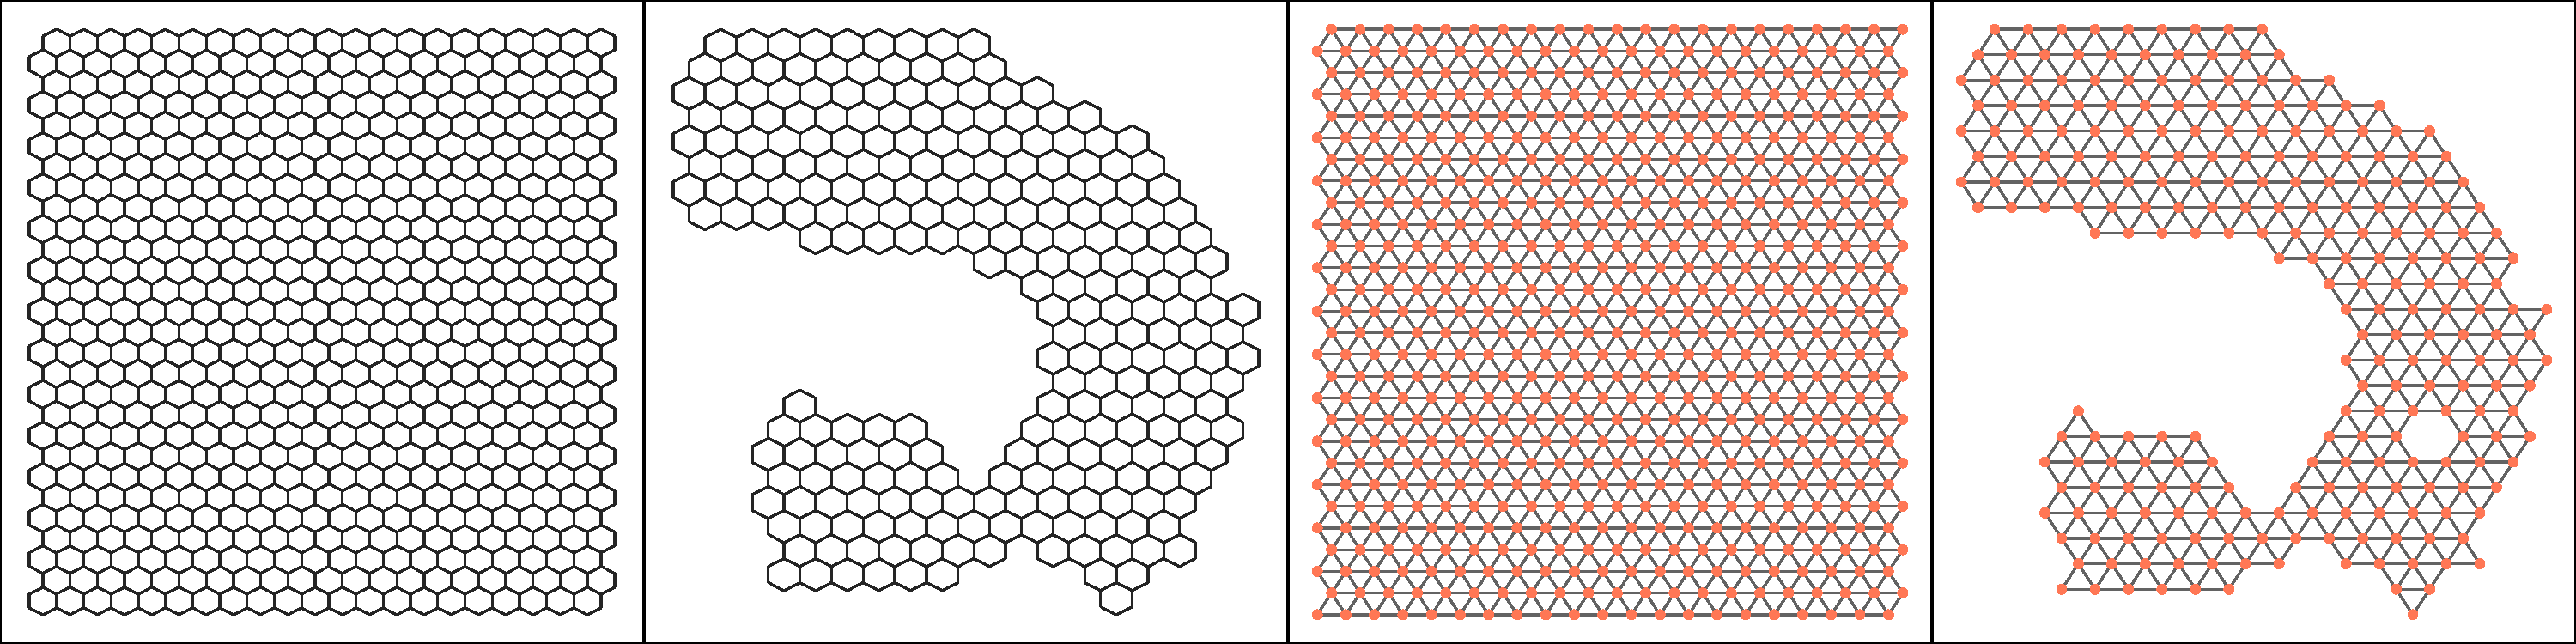
\includegraphics[width=1\linewidth,height=\textheight,keepaspectratio]{chapters/03-chap3_files/figure-pdf/geom-outputs-pdf-1.pdf}

}

\caption{The outputs of \texttt{geom\textbackslash{}\_hexgrid} and
\texttt{geom\textbackslash{}\_trimesh} include: (a) a complete hexagonal
grid, (b) a hexagonal grid that corresponds with the data, (c) a full
grid based on centroid triangulation, and (d) a centroid triangulation
grid that aligns with the data.}

\end{figure}%

\subsubsection{\texorpdfstring{\pD model
visualization}{model visualization}}\label{model-visualization}

To visualize how well the \pD model captures the underlying structure of
the high-dimensional data, we provide a tour of the model in \pD using
the \texttt{show\_langevitour()} function. This function renders a
dynamic projection of both the high-dimensional data and the model using
the \texttt{langevitour} R package
(\citeproc{ref-paul2023}{\textbf{paul2023?}}).

Before plotting, the data needs to be organized into a combined format
through the \texttt{comb\_data\_model()} function. This function takes
three inputs: \texttt{highd\_data} (the high-dimensional observations),
\texttt{model\_highd} (high-dimensional summaries for each bin), and
\texttt{model\_2d} (the hexagonal bin centroids of the model). It
returns a tidy data frame combining both the data and the model.

In this structure, the \texttt{type} variable distinguishes between
original observations (\texttt{"data"}) and the bin-averaged model
representation (\texttt{"model"}).

\begin{Shaded}
\begin{Highlighting}[]
\NormalTok{df\_exe }\OtherTok{\textless{}{-}} \FunctionTok{comb\_data\_model}\NormalTok{(}
  \AttributeTok{highd\_data =}\NormalTok{ scurve, }
  \AttributeTok{model\_highd =}\NormalTok{ df\_bin, }
  \AttributeTok{model\_2d =}\NormalTok{ df\_bin\_centroids}
\NormalTok{  )}
\end{Highlighting}
\end{Shaded}

The \texttt{show\_langevitour()} function then renders the visualization
using the \texttt{langevitour} interface, displaying both types of
points in a dynamic tour. The \texttt{edge\_data} input defines
connections between neighboring bins (i.e., the hexagonal edges) to
visualize the model's structure.

\begin{Shaded}
\begin{Highlighting}[]
\FunctionTok{show\_langevitour}\NormalTok{(}
  \AttributeTok{point\_data =}\NormalTok{ df\_exe, }
  \AttributeTok{edge\_data =}\NormalTok{ trimesh}
\NormalTok{  )}
\end{Highlighting}
\end{Shaded}

\begin{figure}[H]

{\centering 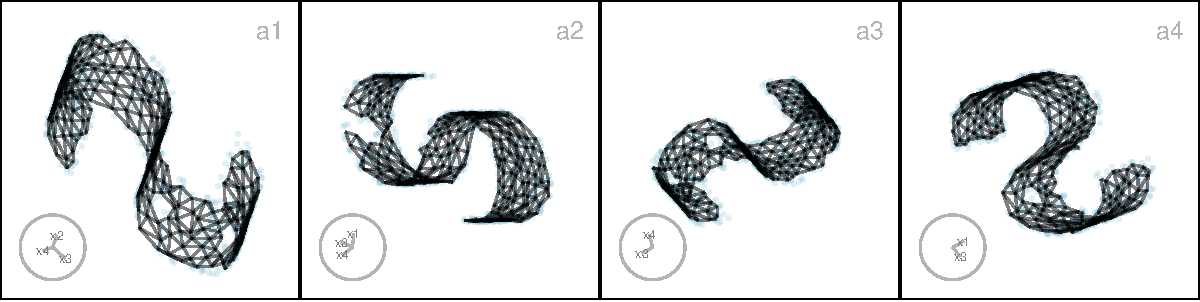
\includegraphics[width=1\linewidth,height=\textheight,keepaspectratio]{chapters/03-chap3_files/figure-pdf/unnamed-chunk-29-1.pdf}

}

\caption{\(2\text{-}D\) projections of the lifted high-dimensional
wireframe model from the \texttt{Scurve} UMAP layout. Each panel
(a1--a4) shows the model (black) overlaid on \texttt{Scurve} data (blue)
in different projections. These views illustrate how the lifted
wireframe model captures the structure of the \texttt{Scurve} data.
Regions with sparse or no data in the UMAP layout are also visible in
the lifted model.}

\end{figure}%

As an alternative to \texttt{langevitour}, users can explore the fitted
\pD model using the \texttt{detourr}
(\citeproc{ref-casper2025}{\textbf{casper2025?}}). The combined data
object from \texttt{comb\_data\_model()} can be passed directly to the
\texttt{detour()} function, where \texttt{tour\_aes()} defines the
projection variables and color mapping. The visualization is rendered
using \texttt{show\_scatter()}, which can display both data points and
the model's structural edges via the \texttt{edges} argument.

\begin{figure}[H]

{\centering 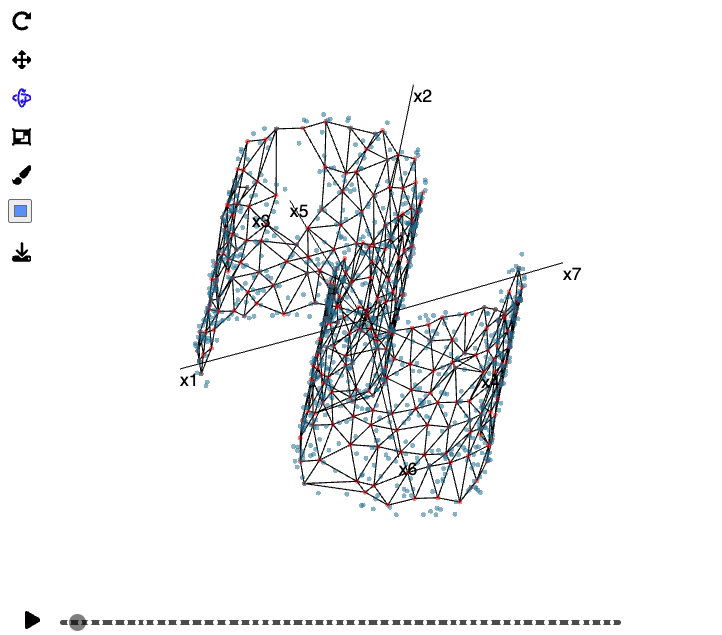
\includegraphics[width=0.5\linewidth,height=\textheight,keepaspectratio]{chapters/../figures/quollr/model_proj1_detourr.png}

}

\caption{Screenshots of the lifted high-dimensional wireframe model from
the \texttt{Scurve} UMAP layout using \texttt{detourr}. Regions with
sparse or no data in the UMAP layout are also visible in the lifted
model.}

\end{figure}%

\begin{figure}[H]

{\centering 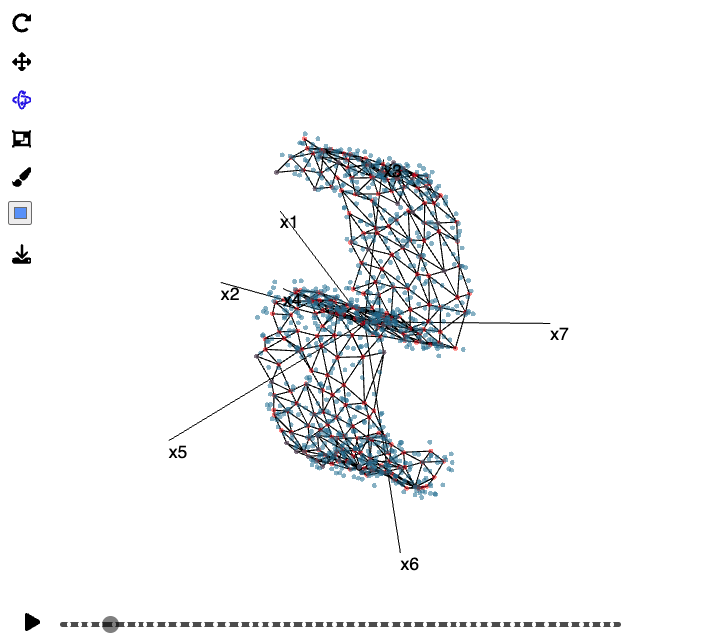
\includegraphics[width=0.5\linewidth,height=\textheight,keepaspectratio]{chapters/../figures/quollr/model_proj2_detourr.png}

}

\caption{Screenshots of the lifted high-dimensional wireframe model from
the \texttt{Scurve} UMAP layout using \texttt{detourr}. Regions with
sparse or no data in the UMAP layout are also visible in the lifted
model.}

\end{figure}%

\begin{Shaded}
\begin{Highlighting}[]
\FunctionTok{detour}\NormalTok{(}
\NormalTok{  df\_exe,}
  \FunctionTok{tour\_aes}\NormalTok{(}
    \AttributeTok{projection =} \FunctionTok{starts\_with}\NormalTok{(}\StringTok{"x"}\NormalTok{),}
    \AttributeTok{colour =}\NormalTok{ type}
\NormalTok{  )}
\NormalTok{) }\SpecialCharTok{|\textgreater{}}
  \FunctionTok{tour\_path}\NormalTok{(}\FunctionTok{grand\_tour}\NormalTok{(}\DecValTok{2}\NormalTok{), }
                    \AttributeTok{max\_bases=}\DecValTok{50}\NormalTok{, }\AttributeTok{fps =} \DecValTok{60}\NormalTok{) }\SpecialCharTok{|\textgreater{}}
  \FunctionTok{show\_scatter}\NormalTok{(}\AttributeTok{axes =} \ConstantTok{TRUE}\NormalTok{, }\AttributeTok{size =} \FloatTok{0.5}\NormalTok{, }\AttributeTok{alpha =} \FloatTok{0.5}\NormalTok{, }
               \AttributeTok{edges =} \FunctionTok{as.matrix}\NormalTok{(trimesh[, }\FunctionTok{c}\NormalTok{(}\StringTok{"from\_reindexed"}\NormalTok{, }\StringTok{"to\_reindexed"}\NormalTok{)]),}
               \AttributeTok{palette =} \FunctionTok{c}\NormalTok{(}\StringTok{"\#66B2CC"}\NormalTok{, }\StringTok{"\#FF7755"}\NormalTok{),}
               \AttributeTok{width =} \StringTok{"600px"}\NormalTok{, }\AttributeTok{height =} \StringTok{"600px"}\NormalTok{)}
\end{Highlighting}
\end{Shaded}

In the resulting interactive visualization, blue points represent the
high-dimensional data, orange points represent the model centroids from
each bin, and the lines between model points reflect the \twoD wireframe
structure mapped to high-dimensional space.

\subsubsection{Link plots}\label{link-plots}

There are mainly two interactive link plots can be generated.

To support interactive evaluation of how well the \pD model captures the
structure of the high-dimensional data, we introduce
\texttt{show\_link\_plots()}. This visualization combines two
complementary views: the nonlinear dimension reduction (NLDR)
representation and a dynamic tour of the model ovelaid the data in the
high-dimensional space. Both views are interactively linked, enabling
users to explore.

Before visualization, the input data must be prepared using the
\texttt{comb\_all\_data\_model()} function. This function combines the
high-dimensional data (\texttt{highd\_data}), the NLDR data
(\texttt{nldr\_data}), and the bin-averaged high-dimensional model
representation (\texttt{model\_highd}) aligned to the \twoD bin layout
(\texttt{model\_2d}):

This combined dataset includes both the original observations and the
bin-level model averages, labeled with a \texttt{type} variable for
distinguishing between them.

\begin{Shaded}
\begin{Highlighting}[]
\NormalTok{df\_exe }\OtherTok{\textless{}{-}} \FunctionTok{comb\_all\_data\_model}\NormalTok{(}
  \AttributeTok{highd\_data =}\NormalTok{ scurve, }
  \AttributeTok{nldr\_data =}\NormalTok{ scurve\_umap, }
  \AttributeTok{model\_highd =}\NormalTok{ df\_bin, }
  \AttributeTok{model\_2d =}\NormalTok{ df\_bin\_centroids}
\NormalTok{  )}
\end{Highlighting}
\end{Shaded}

The function \texttt{show\_link\_plots()} generates two side-by-side,
interactively linked plots; a \twoD NLDR representation, and a dynamic
projection tour in the original high-dimensional space (using the
\texttt{langevitour} package), displaying both the data and the model.
The function takes the output from \texttt{comb\_all\_data\_model()}
(\texttt{point\_data}) and \texttt{edge\_data} which defines connections
between neighboring bins.

These two views are linked using \texttt{crosstalk}, allowing
interactive selection of points in the NLDR plot to highlight
corresponding structures in the \texttt{langevitour} output.

\begin{Shaded}
\begin{Highlighting}[]
\NormalTok{nldrdt\_link }\OtherTok{\textless{}{-}} \FunctionTok{show\_link\_plots}\NormalTok{(}
  \AttributeTok{point\_data =}\NormalTok{ df\_exe, }
  \AttributeTok{edge\_data =}\NormalTok{ trimesh, }
  \AttributeTok{point\_colour =}\NormalTok{ clr\_choice}
\NormalTok{  )}

\FunctionTok{class}\NormalTok{(nldrdt\_link) }\OtherTok{\textless{}{-}} \FunctionTok{c}\NormalTok{(}\FunctionTok{class}\NormalTok{(nldrdt\_link), }\StringTok{"htmlwidget"}\NormalTok{)}

\NormalTok{nldrdt\_link}
\end{Highlighting}
\end{Shaded}

\begin{figure}[H]

{\centering 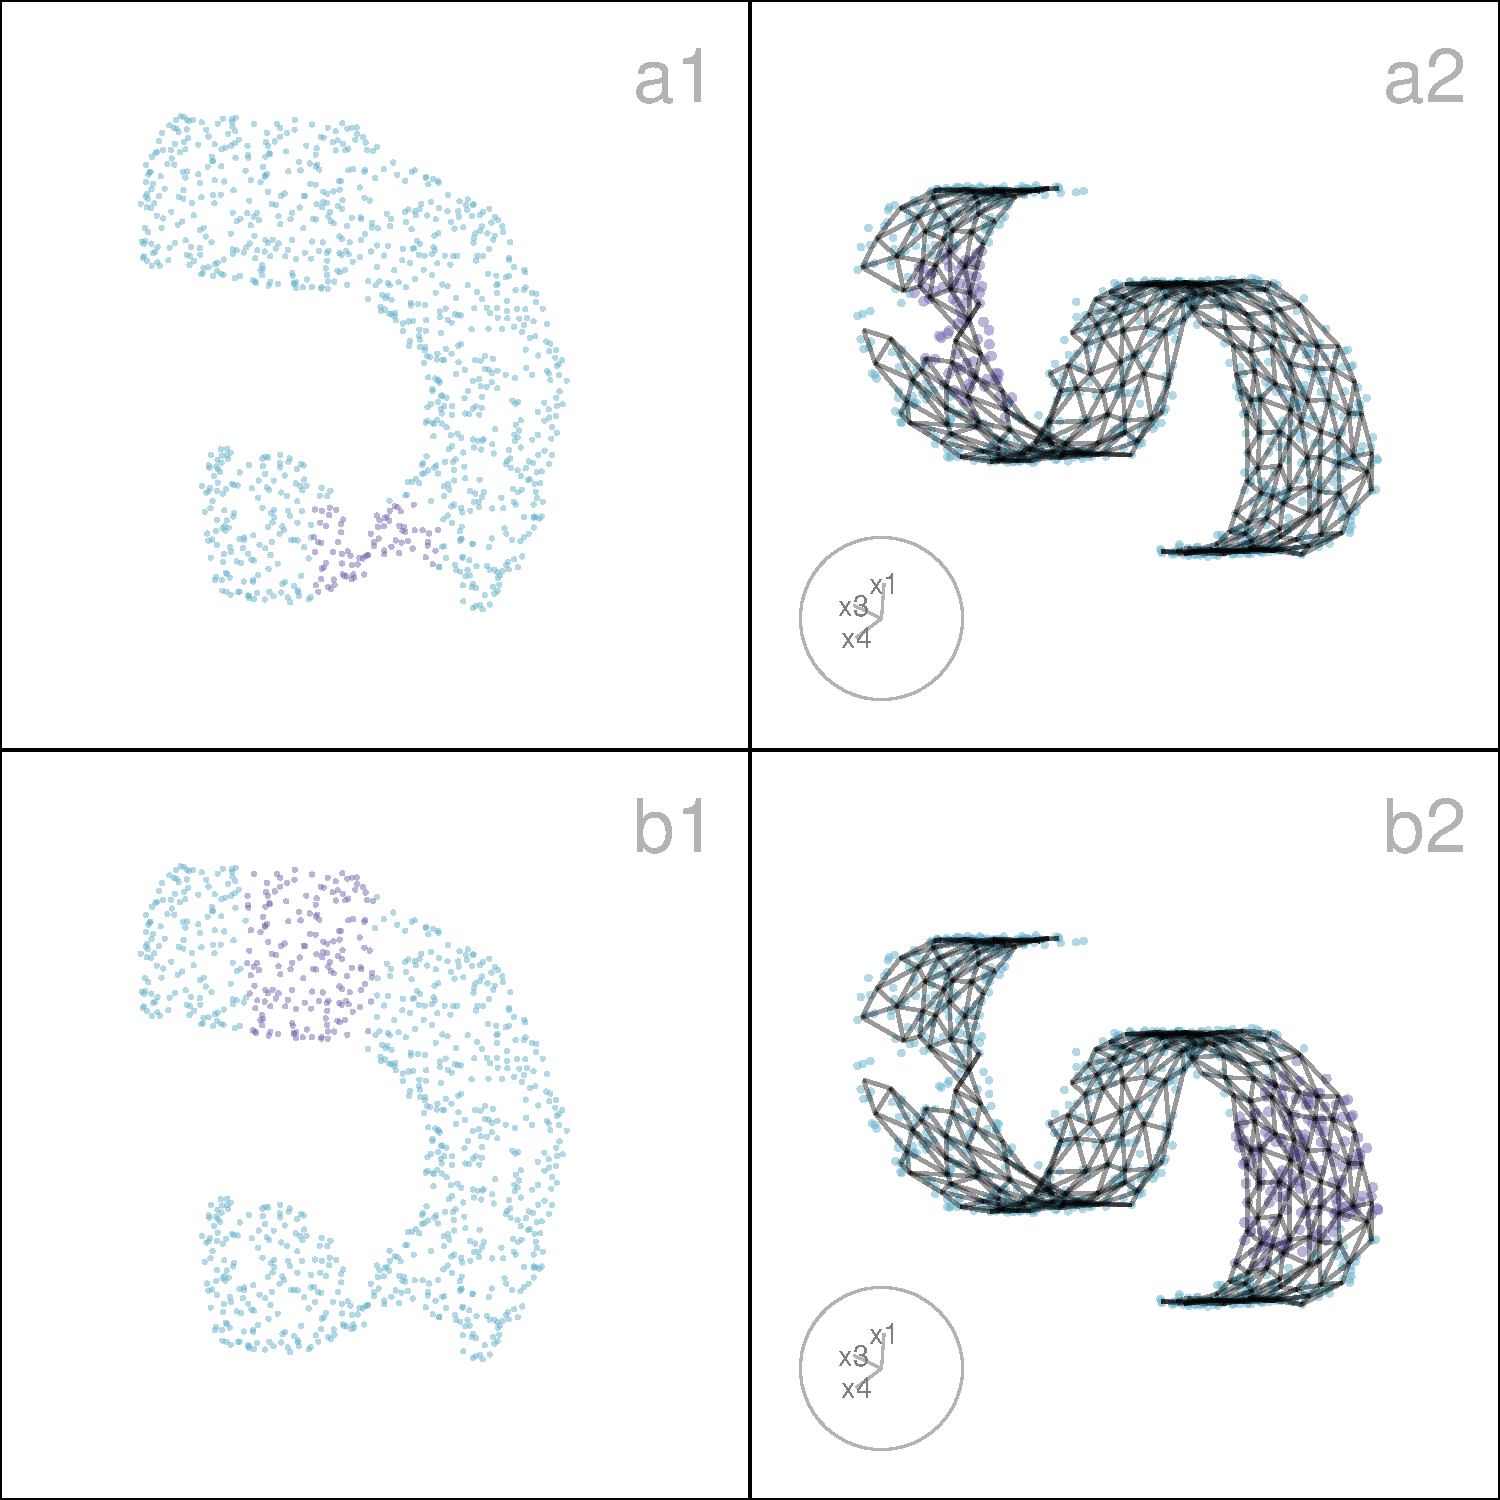
\includegraphics[width=1\linewidth,height=\textheight,keepaspectratio]{chapters/03-chap3_files/figure-pdf/unnamed-chunk-34-1.pdf}

}

\caption{Exploring the correspondence between UMAP layout and
\texttt{Scurve} structure in \(7\text{-}D\). Two sets of plots are
linked: UMAP layout (a1, b1) and projection of \(7\text{-}D\) model and
data (a2, b2). The purple points indicate the selected subsets, which
differ between rows. In (a1), the lower bridge of the \texttt{Scurve} is
highlighted, which corresponds in (a2) to points spanning across both
arms of the high-dimensional structure. In (b1), a different region near
the upper arm of the \texttt{Scurve} is selected, and in (b2) these
points map onto one side of the curved manifold in \(7\text{-}D\)
projection. While the UMAP layout suggests distinct local clusters, the
linked tour views reveal how these selections trace continuous
structures in the \(7\text{-}D\) space, highlighting distortions
introduced by UMAP.}

\end{figure}%

\texttt{show\_error\_link\_plots()} helps to see investigate whether the
model fits the points everywhere or fits better in some places, or
simply mismatches the pattern.

Before visualization, the input data must be prepared using the
\texttt{comb\_all\_data\_model\_error()} function. The function requires
several arguments: points data which contain high-dimensional data
(\texttt{highd\_data}), NLDR data (\texttt{nldr\_data}),
high-dimensional model data (\texttt{model\_highd}), \twoD model data
(\texttt{model\_2d}), and model error (\texttt{error\_data}).

This combined dataset includes both the original observations and the
bin-level model averages, labeled with a \texttt{type} variable for
distinguishing between them.

\begin{Shaded}
\begin{Highlighting}[]
\NormalTok{df\_exe }\OtherTok{\textless{}{-}} \FunctionTok{comb\_all\_data\_model\_error}\NormalTok{(}
  \AttributeTok{highd\_data =}\NormalTok{ scurve, }
  \AttributeTok{nldr\_data =}\NormalTok{ scurve\_umap, }
  \AttributeTok{model\_highd =}\NormalTok{ df\_bin, }
  \AttributeTok{model\_2d =}\NormalTok{ df\_bin\_centroids, }
  \AttributeTok{error\_data =}\NormalTok{ model\_error}
\NormalTok{  )}
\end{Highlighting}
\end{Shaded}

The function \texttt{show\_error\_link\_plots()} generates three
side-by-side, interactively linked plots; a error distribution, a
\twoD NLDR representation, and a dynamic projection tour in the original
high-dimensional space (using the \texttt{langevitour} package),
displaying both the data and the model. The function takes the output
from \texttt{comb\_all\_data\_model\_error()} (\texttt{point\_data}) and
\texttt{edge\_data} which defines connections between neighboring bins.

These two views are linked using \texttt{crosstalk}, allowing
interactive selection of points in the NLDR plot to highlight
corresponding structures in the high-dimensional projection. This setup
facilitates the diagnosis of local distortion, structural artifacts, and
model fit quality.

These three views are linked using \texttt{crosstalk}, allowing
interactive selection of points in error plot and the NLDR plot to
highlight corresponding structures in the \texttt{langevitour} output.

\begin{Shaded}
\begin{Highlighting}[]
\NormalTok{errornldrdt\_link }\OtherTok{\textless{}{-}} \FunctionTok{show\_error\_link\_plots}\NormalTok{(}
  \AttributeTok{point\_data =}\NormalTok{ df\_exe, }
  \AttributeTok{edge\_data =}\NormalTok{ trimesh, }
  \AttributeTok{point\_colour =}\NormalTok{ clr\_choice}
\NormalTok{)}

\FunctionTok{class}\NormalTok{(errornldrdt\_link) }\OtherTok{\textless{}{-}} \FunctionTok{c}\NormalTok{(}\FunctionTok{class}\NormalTok{(errornldrdt\_link), }\StringTok{"htmlwidget"}\NormalTok{)}

\NormalTok{errornldrdt\_link}
\end{Highlighting}
\end{Shaded}

\begin{figure}[H]

{\centering 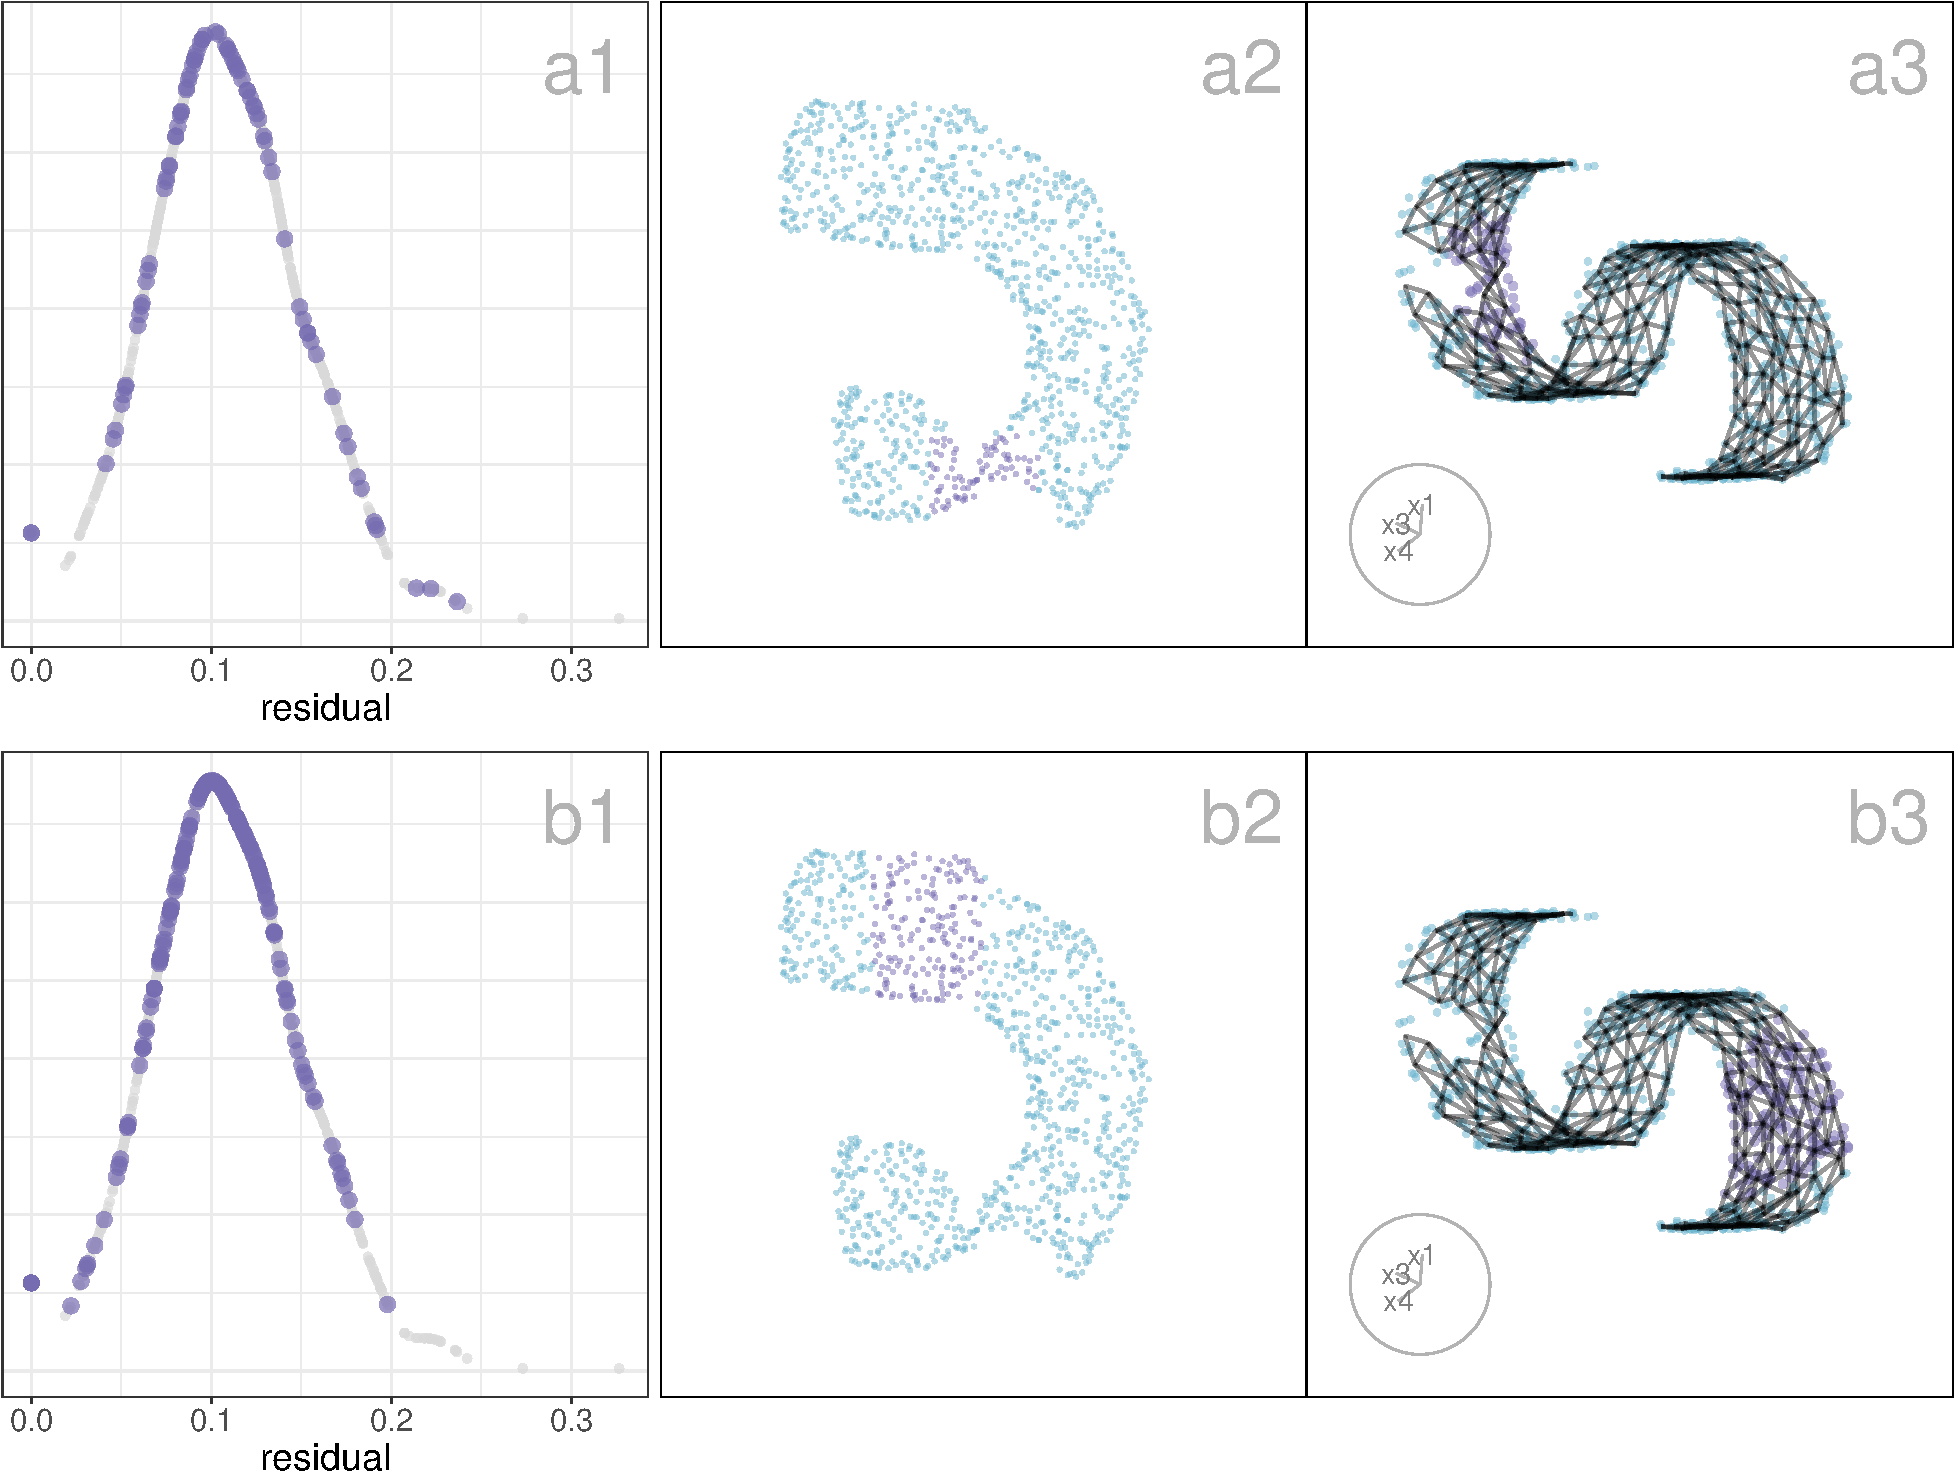
\includegraphics[width=1\linewidth,height=\textheight,keepaspectratio]{chapters/03-chap3_files/figure-pdf/unnamed-chunk-38-1.pdf}

}

\caption{Exploring residuals in relation to UMAP layouts using a
\(7\text{-}D\) \texttt{Scurve} model. Three views are linked:
distribution of residuals (a1, b1), UMAP layout (a2, b2), and projection
of the \(7\text{-}D\) model with data (a3, b3). The purple points
highlight selected subsets of the data, which differ across rows. In the
top row (a1--a3), points with higher residuals (a1) are selected,
corresponding to the sparse bridging region in the UMAP layout (a2) and
the less dense end of the \texttt{Scurve} in the high-dimensional
projection (a3). In the bottom row (b1--b3), points with lower residuals
(b1) are highlighted, which map to one side of the dense region in the
NLDR layout (b2) and to a thicker band of the \texttt{Scurve} in the
projection (b3). This comparison illustrates how residuals can help
diagnose distortions in UMAP, with high-residual points often
concentrated in sparse or stretched regions of the structure.}

\end{figure}%

As an alternative to using \texttt{langevitour}, link plots can also be
generated with the \texttt{detourr} package. In this setup, users can
manually construct the linked visualization using the \texttt{crosstalk}
(\citeproc{ref-joe2023}{\textbf{joe2023?}}) and \texttt{htmltools}
(\citeproc{ref-joe2024}{\textbf{joe2024?}}) packages. The interactive
layout is created by arranging the \twoD NLDR plot (\texttt{nldr\_plt}),
the optional error distribution plot (\texttt{error\_plt}), and the tour
view produced with \texttt{detourr}, side by side within a flexible
grid. The NLDR and error plots are rendered with \texttt{ggplotly()}
(\citeproc{ref-chapman2020}{\textbf{chapman2020?}}) to enable
interactive linking. The \texttt{bscols()} function from
\texttt{crosstalk} manages synchronization across these panels, allowing
for linked brushing and coordinated selection between these interactive
plots.

A two-panel linked plot combining the NLDR view and the tour from
\texttt{detourr} can be created as follows:

\begin{Shaded}
\begin{Highlighting}[]
\NormalTok{detourr\_output }\OtherTok{\textless{}{-}} \FunctionTok{detour}\NormalTok{(}
\NormalTok{  shared\_df,}
  \FunctionTok{tour\_aes}\NormalTok{(}
    \AttributeTok{projection =} \FunctionTok{starts\_with}\NormalTok{(}\StringTok{"x"}\NormalTok{),}
    \AttributeTok{colour =}\NormalTok{ type}
\NormalTok{  )}
\NormalTok{) }\SpecialCharTok{|\textgreater{}}
  \FunctionTok{tour\_path}\NormalTok{(}\FunctionTok{grand\_tour}\NormalTok{(}\DecValTok{2}\NormalTok{), }
                    \AttributeTok{max\_bases=}\DecValTok{50}\NormalTok{, }\AttributeTok{fps =} \DecValTok{60}\NormalTok{) }\SpecialCharTok{|\textgreater{}}
  \FunctionTok{show\_scatter}\NormalTok{(}\AttributeTok{axes =} \ConstantTok{TRUE}\NormalTok{, }\AttributeTok{size =} \DecValTok{1}\NormalTok{, }\AttributeTok{alpha =} \FloatTok{0.8}\NormalTok{, }
               \AttributeTok{edges =} \FunctionTok{as.matrix}\NormalTok{(trimesh[, }\FunctionTok{c}\NormalTok{(}\StringTok{"from\_reindexed"}\NormalTok{, }\StringTok{"to\_reindexed"}\NormalTok{)]),}
               \AttributeTok{palette =} \FunctionTok{c}\NormalTok{(}\StringTok{"\#66B2CC"}\NormalTok{, }\StringTok{"\#FF7755"}\NormalTok{),}
                \AttributeTok{width =} \StringTok{"600px"}\NormalTok{, }\AttributeTok{height =} \StringTok{"600px"}\NormalTok{)}
\end{Highlighting}
\end{Shaded}

\begin{Shaded}
\begin{Highlighting}[]
\NormalTok{lndet\_link }\OtherTok{\textless{}{-}}\NormalTok{ crosstalk}\SpecialCharTok{::}\FunctionTok{bscols}\NormalTok{(}
\NormalTok{    htmltools}\SpecialCharTok{::}\FunctionTok{div}\NormalTok{(}\AttributeTok{style=}\StringTok{"display: grid; grid{-}template{-}columns: 1fr 1fr;"}\NormalTok{,}
\NormalTok{                   nldr\_plt,}
\NormalTok{                   htmltools}\SpecialCharTok{::}\FunctionTok{div}\NormalTok{(}\AttributeTok{style =} \StringTok{"margin{-}top: 20px;"}\NormalTok{, detourr\_output)}
\NormalTok{    ),}
    \AttributeTok{device =} \StringTok{"xs"}
\NormalTok{  )}


\FunctionTok{class}\NormalTok{(lndet\_link) }\OtherTok{\textless{}{-}} \FunctionTok{c}\NormalTok{(}\FunctionTok{class}\NormalTok{(lndet\_link), }\StringTok{"htmlwidget"}\NormalTok{)}

\NormalTok{lndet\_link}
\end{Highlighting}
\end{Shaded}

\begin{figure}[H]

{\centering 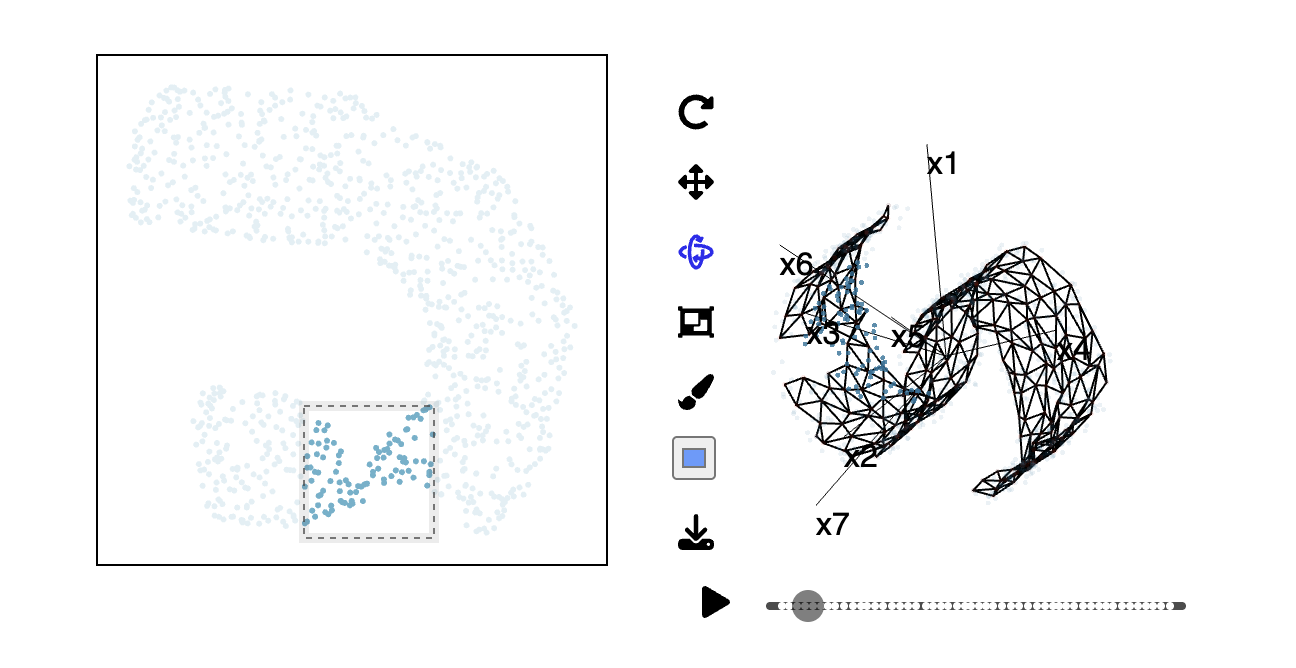
\includegraphics[width=1\linewidth,height=\textheight,keepaspectratio]{chapters/../figures/quollr/model_link_proj1_detourr.png}

}

\caption{Screenshots of the link plots showing the relationship between
the NLDR layout (left) and the fitted model overlaid with the data in
\(7\text{-}D\) (right) using \texttt{detourr}.}

\end{figure}%

\begin{figure}[H]

{\centering 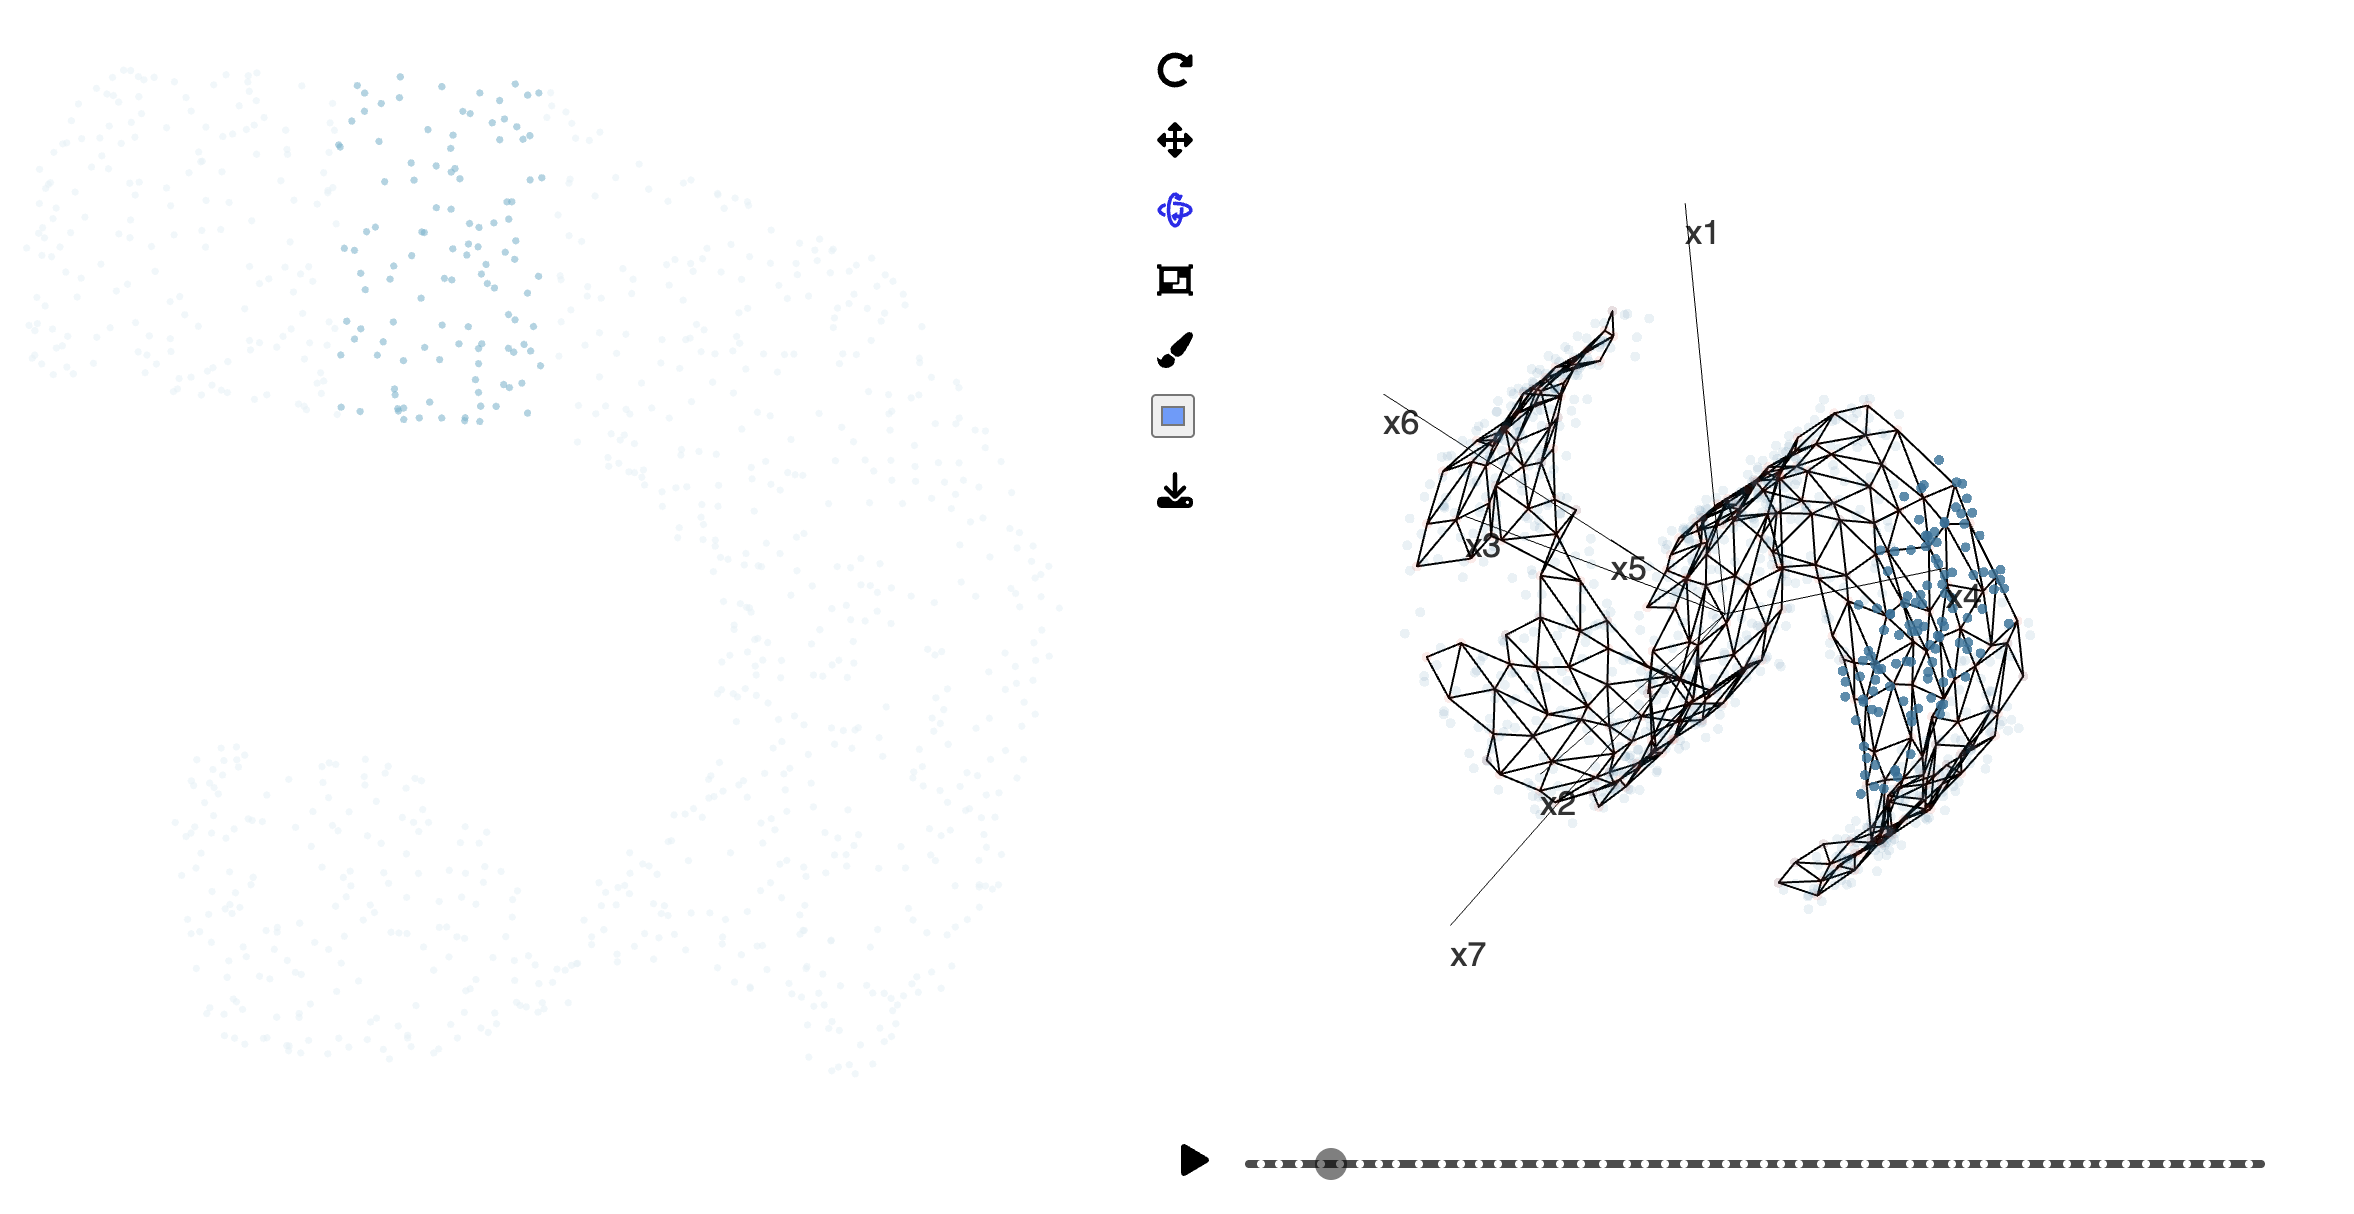
\includegraphics[width=1\linewidth,height=\textheight,keepaspectratio]{chapters/../figures/quollr/model_link_proj2_detourr.png}

}

\caption{Screenshots of the link plots showing the relationship between
the NLDR layout (left) and the fitted model overlaid with the data in
\(7\text{-}D\) (right) using \texttt{detourr}.}

\end{figure}%

For analyses that include model error visualization, a three-panel view
can be constructed by adding the error distribution plot
(\texttt{error\_plt}):

\begin{Shaded}
\begin{Highlighting}[]
\NormalTok{detourr\_output }\OtherTok{\textless{}{-}} \FunctionTok{detour}\NormalTok{(}
\NormalTok{  shared\_df,}
  \FunctionTok{tour\_aes}\NormalTok{(}
    \AttributeTok{projection =} \FunctionTok{starts\_with}\NormalTok{(}\StringTok{"x"}\NormalTok{),}
    \AttributeTok{colour =}\NormalTok{ type}
\NormalTok{  )}
\NormalTok{) }\SpecialCharTok{|\textgreater{}}
  \FunctionTok{tour\_path}\NormalTok{(}\FunctionTok{grand\_tour}\NormalTok{(}\DecValTok{2}\NormalTok{), }
                    \AttributeTok{max\_bases=}\DecValTok{50}\NormalTok{, }\AttributeTok{fps =} \DecValTok{60}\NormalTok{) }\SpecialCharTok{|\textgreater{}}
  \FunctionTok{show\_scatter}\NormalTok{(}\AttributeTok{axes =} \ConstantTok{TRUE}\NormalTok{, }\AttributeTok{size =} \DecValTok{1}\NormalTok{, }\AttributeTok{alpha =} \FloatTok{0.8}\NormalTok{, }
               \AttributeTok{edges =} \FunctionTok{as.matrix}\NormalTok{(trimesh[, }\FunctionTok{c}\NormalTok{(}\StringTok{"from\_reindexed"}\NormalTok{, }\StringTok{"to\_reindexed"}\NormalTok{)]),}
               \AttributeTok{palette =} \FunctionTok{c}\NormalTok{(}\StringTok{"\#66B2CC"}\NormalTok{, }\StringTok{"\#FF7755"}\NormalTok{),}
                \AttributeTok{width =} \StringTok{"500px"}\NormalTok{, }\AttributeTok{height =} \StringTok{"500px"}\NormalTok{)}

\NormalTok{erlndet\_link }\OtherTok{\textless{}{-}}\NormalTok{ crosstalk}\SpecialCharTok{::}\FunctionTok{bscols}\NormalTok{(}
\NormalTok{  htmltools}\SpecialCharTok{::}\FunctionTok{div}\NormalTok{(}
    \AttributeTok{style =} \StringTok{"display: grid; grid{-}template{-}columns: 1fr 1fr 1fr;"}\NormalTok{,}
\NormalTok{    error\_plt, }
\NormalTok{    nldr\_plt,}
\NormalTok{    htmltools}\SpecialCharTok{::}\FunctionTok{div}\NormalTok{(}\AttributeTok{style =} \StringTok{"margin{-}top: 20px;"}\NormalTok{, detourr\_output)}
\NormalTok{  ),}
  \AttributeTok{device =} \StringTok{"xs"}
\NormalTok{)}

\FunctionTok{class}\NormalTok{(erlndet\_link) }\OtherTok{\textless{}{-}} \FunctionTok{c}\NormalTok{(}\FunctionTok{class}\NormalTok{(erlndet\_link), }\StringTok{"htmlwidget"}\NormalTok{)}

\NormalTok{erlndet\_link}
\end{Highlighting}
\end{Shaded}

\begin{figure}[H]

{\centering 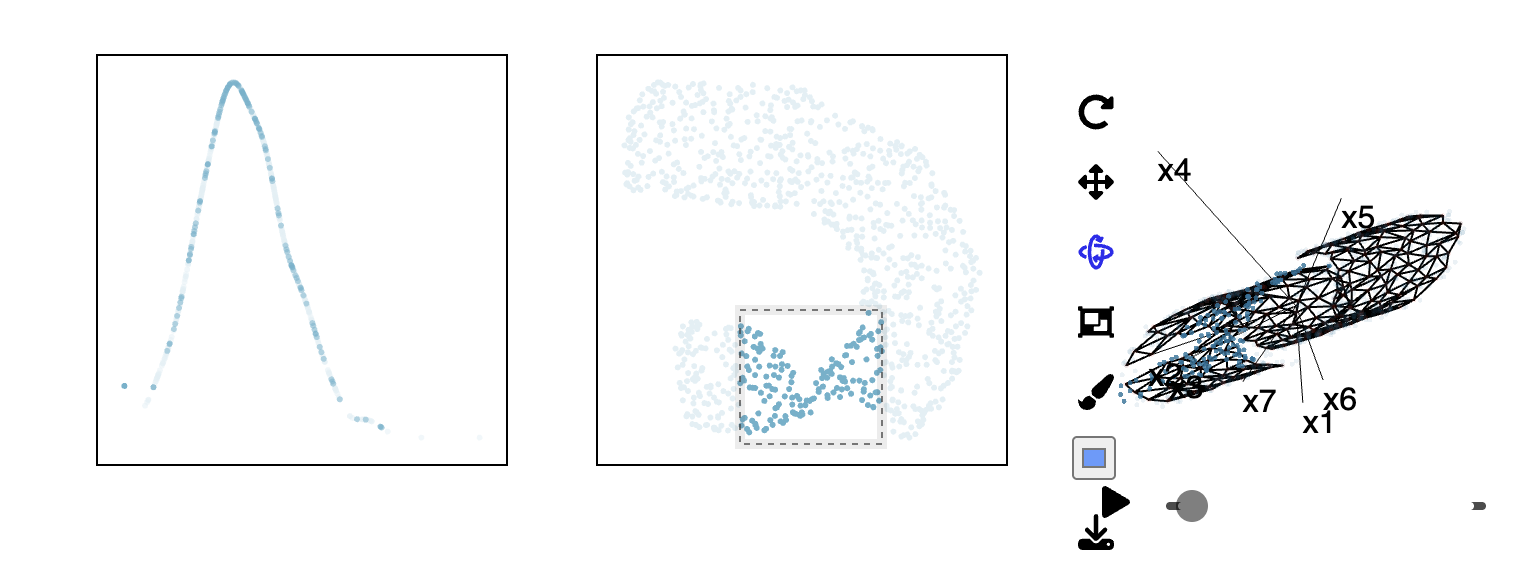
\includegraphics[width=1\linewidth,height=\textheight,keepaspectratio]{chapters/../figures/quollr/model_link_error_proj1_detourr.png}

}

\caption{Screenshots of the link plots showing the relationship between
the distribution of residuals (left), NLDR layout (middle) and the
fitted model overlaid with the data in \(7\text{-}D\) (right) using
\texttt{detourr}.}

\end{figure}%

\begin{figure}[H]

{\centering 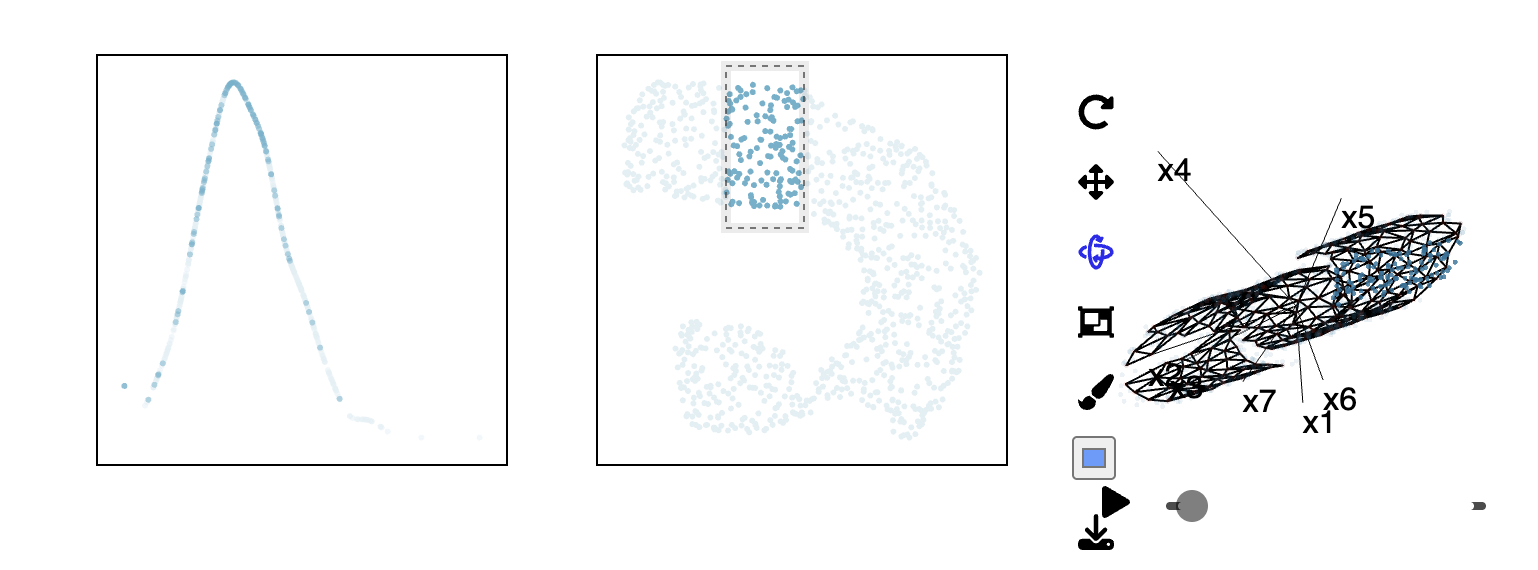
\includegraphics[width=1\linewidth,height=\textheight,keepaspectratio]{chapters/../figures/quollr/model_link_error_proj2_detourr.png}

}

\caption{Screenshots of the link plots showing the relationship between
the distribution of residuals (left), NLDR layout (middle) and the
fitted model overlaid with the data in \(7\text{-}D\) (right) using
\texttt{detourr}.}

\end{figure}%

\section{Application}\label{application}

Single-cell RNA sequencing (scRNA-seq) is a popular and powerful
technology that allows you to profile the whole transcriptome of a large
number of individual cells
(\citeproc{ref-andrews2021}{\textbf{andrews2021?}}).

Clustering of single-cell data is used to identify groups of cells with
similar expression profiles. NLDR often used to summarise the discovered
clusters, and help to understand the results. The purpose of this
example is to \emph{illustrate how to use our method to help decide on
an appropriate NLDR layout that accurately represents the data}.

Limb muscle cells of mice in
(\citeproc{ref-tabula2018}{\textbf{tabula2018?}}) are examined. There
are \(1067\) single cells, with \(14997\) gene expressions. Following
their pre-processing, different NLDR methods were performed using ten
principal components. Figure @ref(fig:limb-rwbss) (b) is the
reproduction of the published plot. The question is whether this
accurately represents the cluster structure in the data. Our method help
to provide a better \twoD layout.

\begin{Shaded}
\begin{Highlighting}[]
\NormalTok{design }\OtherTok{\textless{}{-}} \FunctionTok{gen\_design}\NormalTok{(}\AttributeTok{n\_right =} \DecValTok{6}\NormalTok{, }\AttributeTok{ncol\_right =} \DecValTok{2}\NormalTok{)}

\FunctionTok{plot\_hbe\_layouts}\NormalTok{(}\AttributeTok{plots =} \FunctionTok{list}\NormalTok{(error\_plot\_limb, nldr1, }
\NormalTok{                               nldr2, nldr3, nldr4, }
\NormalTok{                               nldr5, nldr6), }\AttributeTok{design =}\NormalTok{ design)}
\end{Highlighting}
\end{Shaded}

\begin{figure}[H]

{\centering 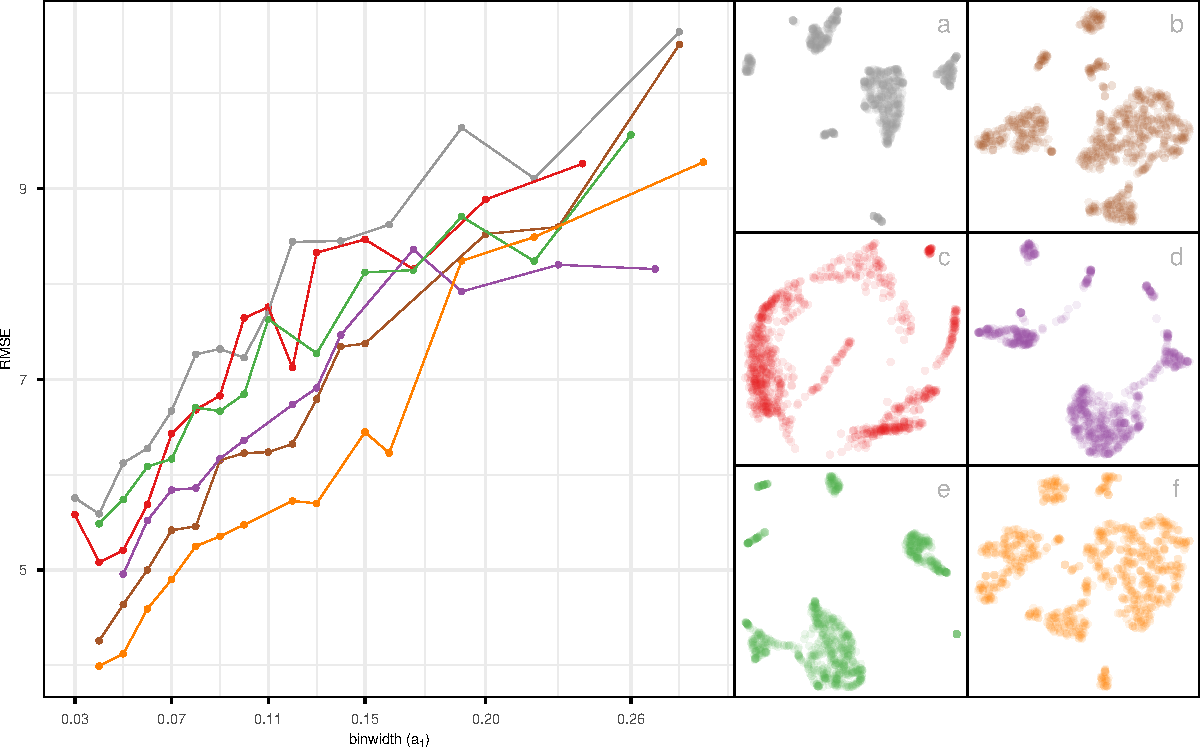
\includegraphics[width=1\linewidth,height=\textheight,keepaspectratio]{chapters/03-chap3_files/figure-pdf/limb-rwbss-1.pdf}

}

\caption{Assessing which of the 6 NLDR layouts on the limb muscle data
is the better representation using RWBSS for varying binwidth (\(a_1\)).
Colour used for the lines and points in the left plot and in the
scatterplots represents NLDR layout (a-f). Layout d is perform well at
large binwidth (where the binwidth is not enough to capture the data
struture) and poorly as bin width decreases. Layout f is the best
choice.\label{fig:limb-rwbss}}

\end{figure}%

\begin{figure}[H]

{\centering 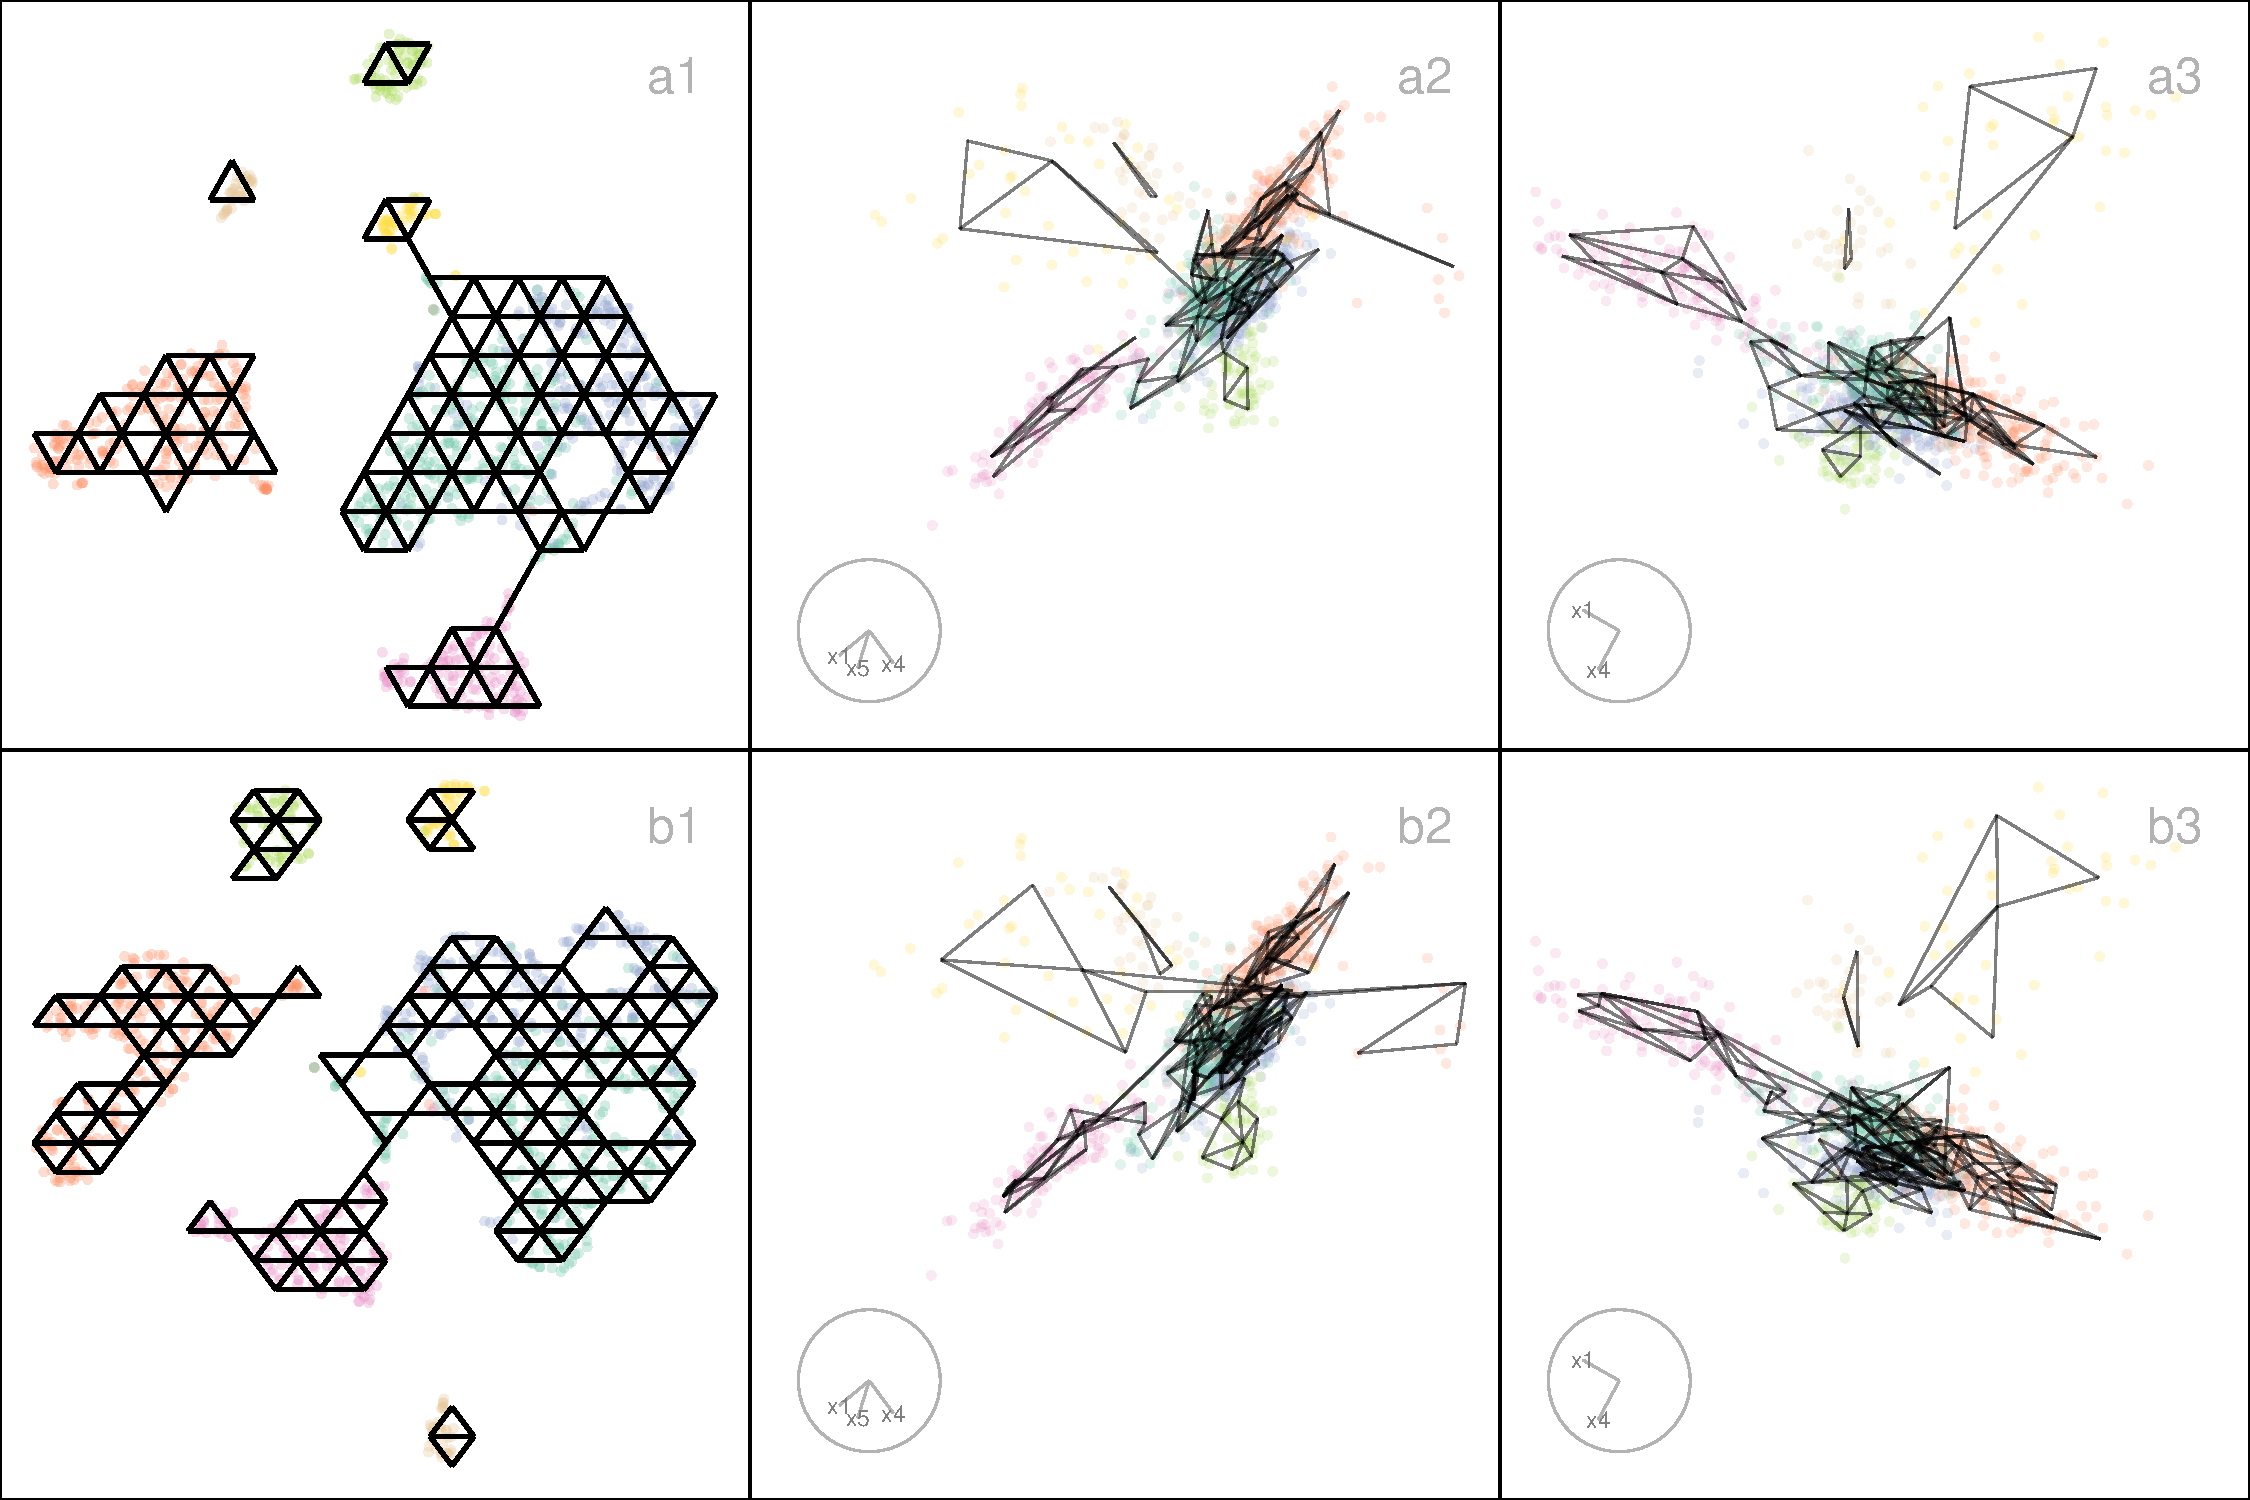
\includegraphics[width=1\linewidth,height=\textheight,keepaspectratio]{chapters/03-chap3_files/figure-pdf/model-limb-1.pdf}

}

\caption{Compare the published \(2\text{-}D\) layout (Figure
\ref{fig:limb-rwbss}b) and the \(2\text{-}D\) layout selected (Figure
\ref{fig:limb-rwbss}f) by RWBSS plot (Figure \ref{fig:limb-rwbss}) from
the tSNE, UMAP, PHATE, TriMAP, and PaCMAP with different
hyper-parameters. The Limb muscle data (\(n =  1067\)) has seven close
different shaped clusters in \(10\text{-}D\).}

\end{figure}%

\section{Discussion}\label{discussion}

The \texttt{quollr} package introduces a new framework for interpreting
NLDR outputs by fitting a geometric wireframe model in \twoD and lifting
it into high-dimensional space. This lifted model provides a direct way
to assess how well a \twoD layout, produced by methods such as tSNE,
UMAP, PHATE, TriMAP, or PaCMAP, preserves the structure of the original
high-dimensional data. The approach offers both numerical and visual
diagnostics to support the selection of NLDR methods and tuning
hyper-parameters that produce the most accurate \twoD representations.

In contrast to the common practice of visually inspecting scatterplots
for clusters or patterns, \texttt{quollr} provides a quantitative route
for evaluation. It enables the computation of RWBSS and residuals
between the original high-dimensional data and the lifted model,
offering interpretable diagnostics. These diagnostics are complemented
by interactive linked plots and high-dimensional dynamic visualizations
using the \texttt{langevitour} package, allowing users to inspect where
the model fits well and where it does not.

To support efficient computation, particularly for large-scale datasets,
several core functions in \texttt{quollr} are implemented in C++ using
\texttt{Rcpp} and \texttt{RcppArmadillo}. These include functions for
computing Euclidean distances in high-dimensional and \twoD space,
identifying nearest centroids, calculating residual errors, and
generating polygonal coordinates of hexagons. For instance,
\texttt{compute\_highd\_dist()} accelerates nearest neighbor lookup in
high-dimensional space, \texttt{compute\_errors()} calculates RWBSS and
total absolute error efficiently, and \texttt{calc\_2d\_dist\_cpp()}
speeds up distance calculations in \twoD. Additionally,
\texttt{gen\_hex\_coord\_cpp()} constructs the coordinates for hexagonal
bins based on their centroids with minimal overhead. These optimizations
result in substantial performance gains compared to native R
implementations, making the package responsive even when used in
interactive contexts or on large datasets such as single-cell
transcriptomic profiles.

The modular structure of the package is designed to support both
flexibility and reproducibility. Users can access individual functions
to control each step of the pipeline such as scaling, binning, and
triangulation or use the main function \texttt{fit\_highd\_model()} for
end-to-end model construction. The diagnostics can be used not only to
compare NLDR methods but also to tune binning parameters, assess layout
stability, and detect local distortions in the embedding.

There are several avenues for future development. While hexagonal
binning provides a regular structure conducive to modeling, alternative
spatial discretizations (e.g., adaptive binning or density-aware
tessellations) could be explored to better capture varying data
densities. Expanding support for additional distance metrics in the
lifting and prediction steps may improve performance across different
domains. Additionally, statistical inference tools could be introduced
to assess the stability and robustness of the fitted model, which would
enhance interpretability and confidence in the outcomes.

\section{Acknowledgements}\label{acknowledgements-1}

The source code for reproducing this paper can be found at:
\url{https://github.com/JayaniLakshika/paper-quollr}. This article is
created using \CRANpkg{knitr}
(\citeproc{ref-yihui2015}{\textbf{yihui2015?}}) and \CRANpkg{rmarkdown}
(\citeproc{ref-yihui2018}{\textbf{yihui2018?}}) in R with the
\texttt{rjtools::rjournal\_article} template. These \texttt{R} packages
were used for this work: \texttt{cli}
(\citeproc{ref-gabor2025}{\textbf{gabor2025?}}), \texttt{dplyr}
(\citeproc{ref-hadley2023}{Wickham 2023}), \texttt{ggplot2}
(\citeproc{ref-hadley2016}{\textbf{hadley2016?}}), \texttt{interp}
(\textgreater= 1.1-6)
(\citeproc{ref-albrecht2024}{\textbf{albrecht2024?}}),
\texttt{langevitour} (\citeproc{ref-paul2023}{\textbf{paul2023?}}),
\texttt{proxy}(\citeproc{ref-david2022}{\textbf{david2022?}}),
\texttt{stats} (\citeproc{ref-core2025}{\textbf{core2025?}}),
\texttt{tibble} (\citeproc{ref-kirill2023}{\textbf{kirill2023?}}),
\texttt{tidyselect} (\citeproc{ref-lionel2024}{\textbf{lionel2024?}}),
\texttt{crosstalk} (\citeproc{ref-joe2023}{\textbf{joe2023?}}),
\texttt{plotly} (\citeproc{ref-chapman2020}{\textbf{chapman2020?}}),
\texttt{htmltools} (\citeproc{ref-joe2024}{\textbf{joe2024?}}),
\texttt{kableExtra} (\citeproc{ref-hao2024}{Zhu 2024}),
\texttt{patchwork} (\citeproc{ref-thomas2024}{Pedersen 2024}), and
\texttt{readr} (\citeproc{ref-hadley2024}{\textbf{hadley2024?}}).

\bookmarksetup{startatroot}

\chapter{cardinalR: Generating interesting high-dimensional data
structures}\label{sec-fourth-paper}

A high-dimensional dataset is one where each observation is described by
many features, or dimensions, with associations between them. These
datasets contain nonlinear manifolds in image and speech recognition,
clusters in genomics and forensic analysis, and sparse distributions in
text mining. Data with a variety of structures can be generated using
mathematical functions and statistical distributions to create test
datasets. High-dimensional data structures are useful for testing,
validating, and improving algorithms used in dimensionality reduction,
clustering, machine learning, and visualization. Their controlled
complexity allows researchers to understand challenges posed in data
analysis and helps to develop robust analytical methods across diverse
scientific fields like bioinformatics, machine learning, and forensic
science. Functions to generate a large variety of structures in high
dimensions are organized into the R package \texttt{cardinalR}, along
with some already generated examples, adding to the existing toolset of
benchmark datasets for evaluating algorithms.

\section{Introduction}\label{introduction-2}

Generating synthetic datasets with clearly defined geometric properties
is useful for evaluating and benchmarking algorithms in various fields,
such as machine learning, data mining, and computational biology.
Researchers often need to generate data with specific dimensions, noise
characteristics, and complex underlying structures to test the
performance and robustness of their methods. There are numerous packages
available in R for generating synthetic data, each designed with unique
characteristics and focus areas.The \texttt{geozoo} package
((\citeproc{ref-barret2016}{\textbf{barret2016?}})) offers a large
collection of geometric objects, allowing users to create and analyze
specific shapes, primarily in lower-dimensional spaces. The package is
\texttt{snedata} ((\citeproc{ref-james2025}{\textbf{james2025?}})),
which provides tools for generating simplified datasets useful for
evaluating dimensionality reduction techniques like tSNE, often focusing
on understanding and evaluating low-dimensional embeddings of complex
data structures. Additionally, \texttt{splatter}
((\citeproc{ref-luke2017}{\textbf{luke2017?}})) is designed to simulate
complex biological data, capturing field-specific nuances such as batch
effects and differential expression. In contrast, \texttt{mlbench}
((\citeproc{ref-friedrich2024}{\textbf{friedrich2024?}})) includes a
collection of well-known benchmark datasets commonly associated with
established classification or regression challenges. The
\texttt{surreal} package
((\citeproc{ref-james2024}{\textbf{james2024?}})) implements the
``Residual (Sur)Realism'' algorithm
((\citeproc{ref-leonard2007}{\textbf{leonard2007?}})) to generate
datasets that embed hidden images or text into residual plots, providing
engaging visual demonstrations for teaching model diagnostics.
Meanwhile, the \texttt{DHARMa} package
((\citeproc{ref-florian2024}{\textbf{florian2024?}})) adopts a
simulation-based approach to create scaled quantile residuals for
generalized linear (mixed) models and related frameworks, supporting
model diagnostics through intuitive residuals, plots, and tests for
common misspecification issues.

While these packages are valuable, their scope is often limited to
specific applications or low-dimensional structures. To address this
gap, this paper introduces the \texttt{cardinalR} R package. This
package provides a collection of functions designed to generate
customizable data structures in any number of dimensions, starting from
basic geometric shapes. \texttt{cardinalR} offers important
functionalities that extend beyond the capabilities of existing tools,
allowing users to: (i) construct high-dimensional datasets based on
geometric shapes, including the option to enhance dimensionality by
adding controlled noise dimensions; (ii) introduce adjustable levels of
background noise to these structures; and (iii) combine high-dimensional
datasets into a single multi-faceted, clustered dataset in a space of
arbitrary dimension. By using clearly defined geometric shapes and
controllable characteristics such as number of dimensions, sample size;
\texttt{cardinalR} allows researchers to generate transparent and
interpretable synthetic datasets useful for evaluating the performance
of nonlinear dimensionality reduction (NLDR) methods, clustering
algorithms, and visualization techniques. Moreover, these datasets can
serve as benchmark examples for exploring how different algorithmic
choices affect the identification or representation of cluster and
manifold structures in high-dimensional spaces.

The paper is organized as follows. In the next section, we introduce the
implementation of the \texttt{cardinalR} package on GitHub, including a
demonstration of the package's key functions. We illustrate how a
clustering data structure affects the dimension reductions in the
Application section. Finally, we give a brief conclusion of the paper
and discuss potential opportunities for the use of our data collection.

\section{Implementation}\label{implementation-1}

The \texttt{cardinalR} package is built on a modular framework where
individual geometric generators (e.g., Gaussian, cone, sphere) create
well-defined shapes. The main function, \texttt{gen\_multicluster()},
combines these shapes into a single dataset by applying scaling,
rotation, and translation through \texttt{gen\_rotation()}. Each
generated shape is assigned a unique cluster label. This design allows
flexible construction of complex, high-dimensional structures for
evaluating clustering and dimension reduction methods. Figure
@ref(fig:workflow) illustrates the workflow of
\texttt{gen\_multicluster()}.

\begin{figure}[H]

{\centering 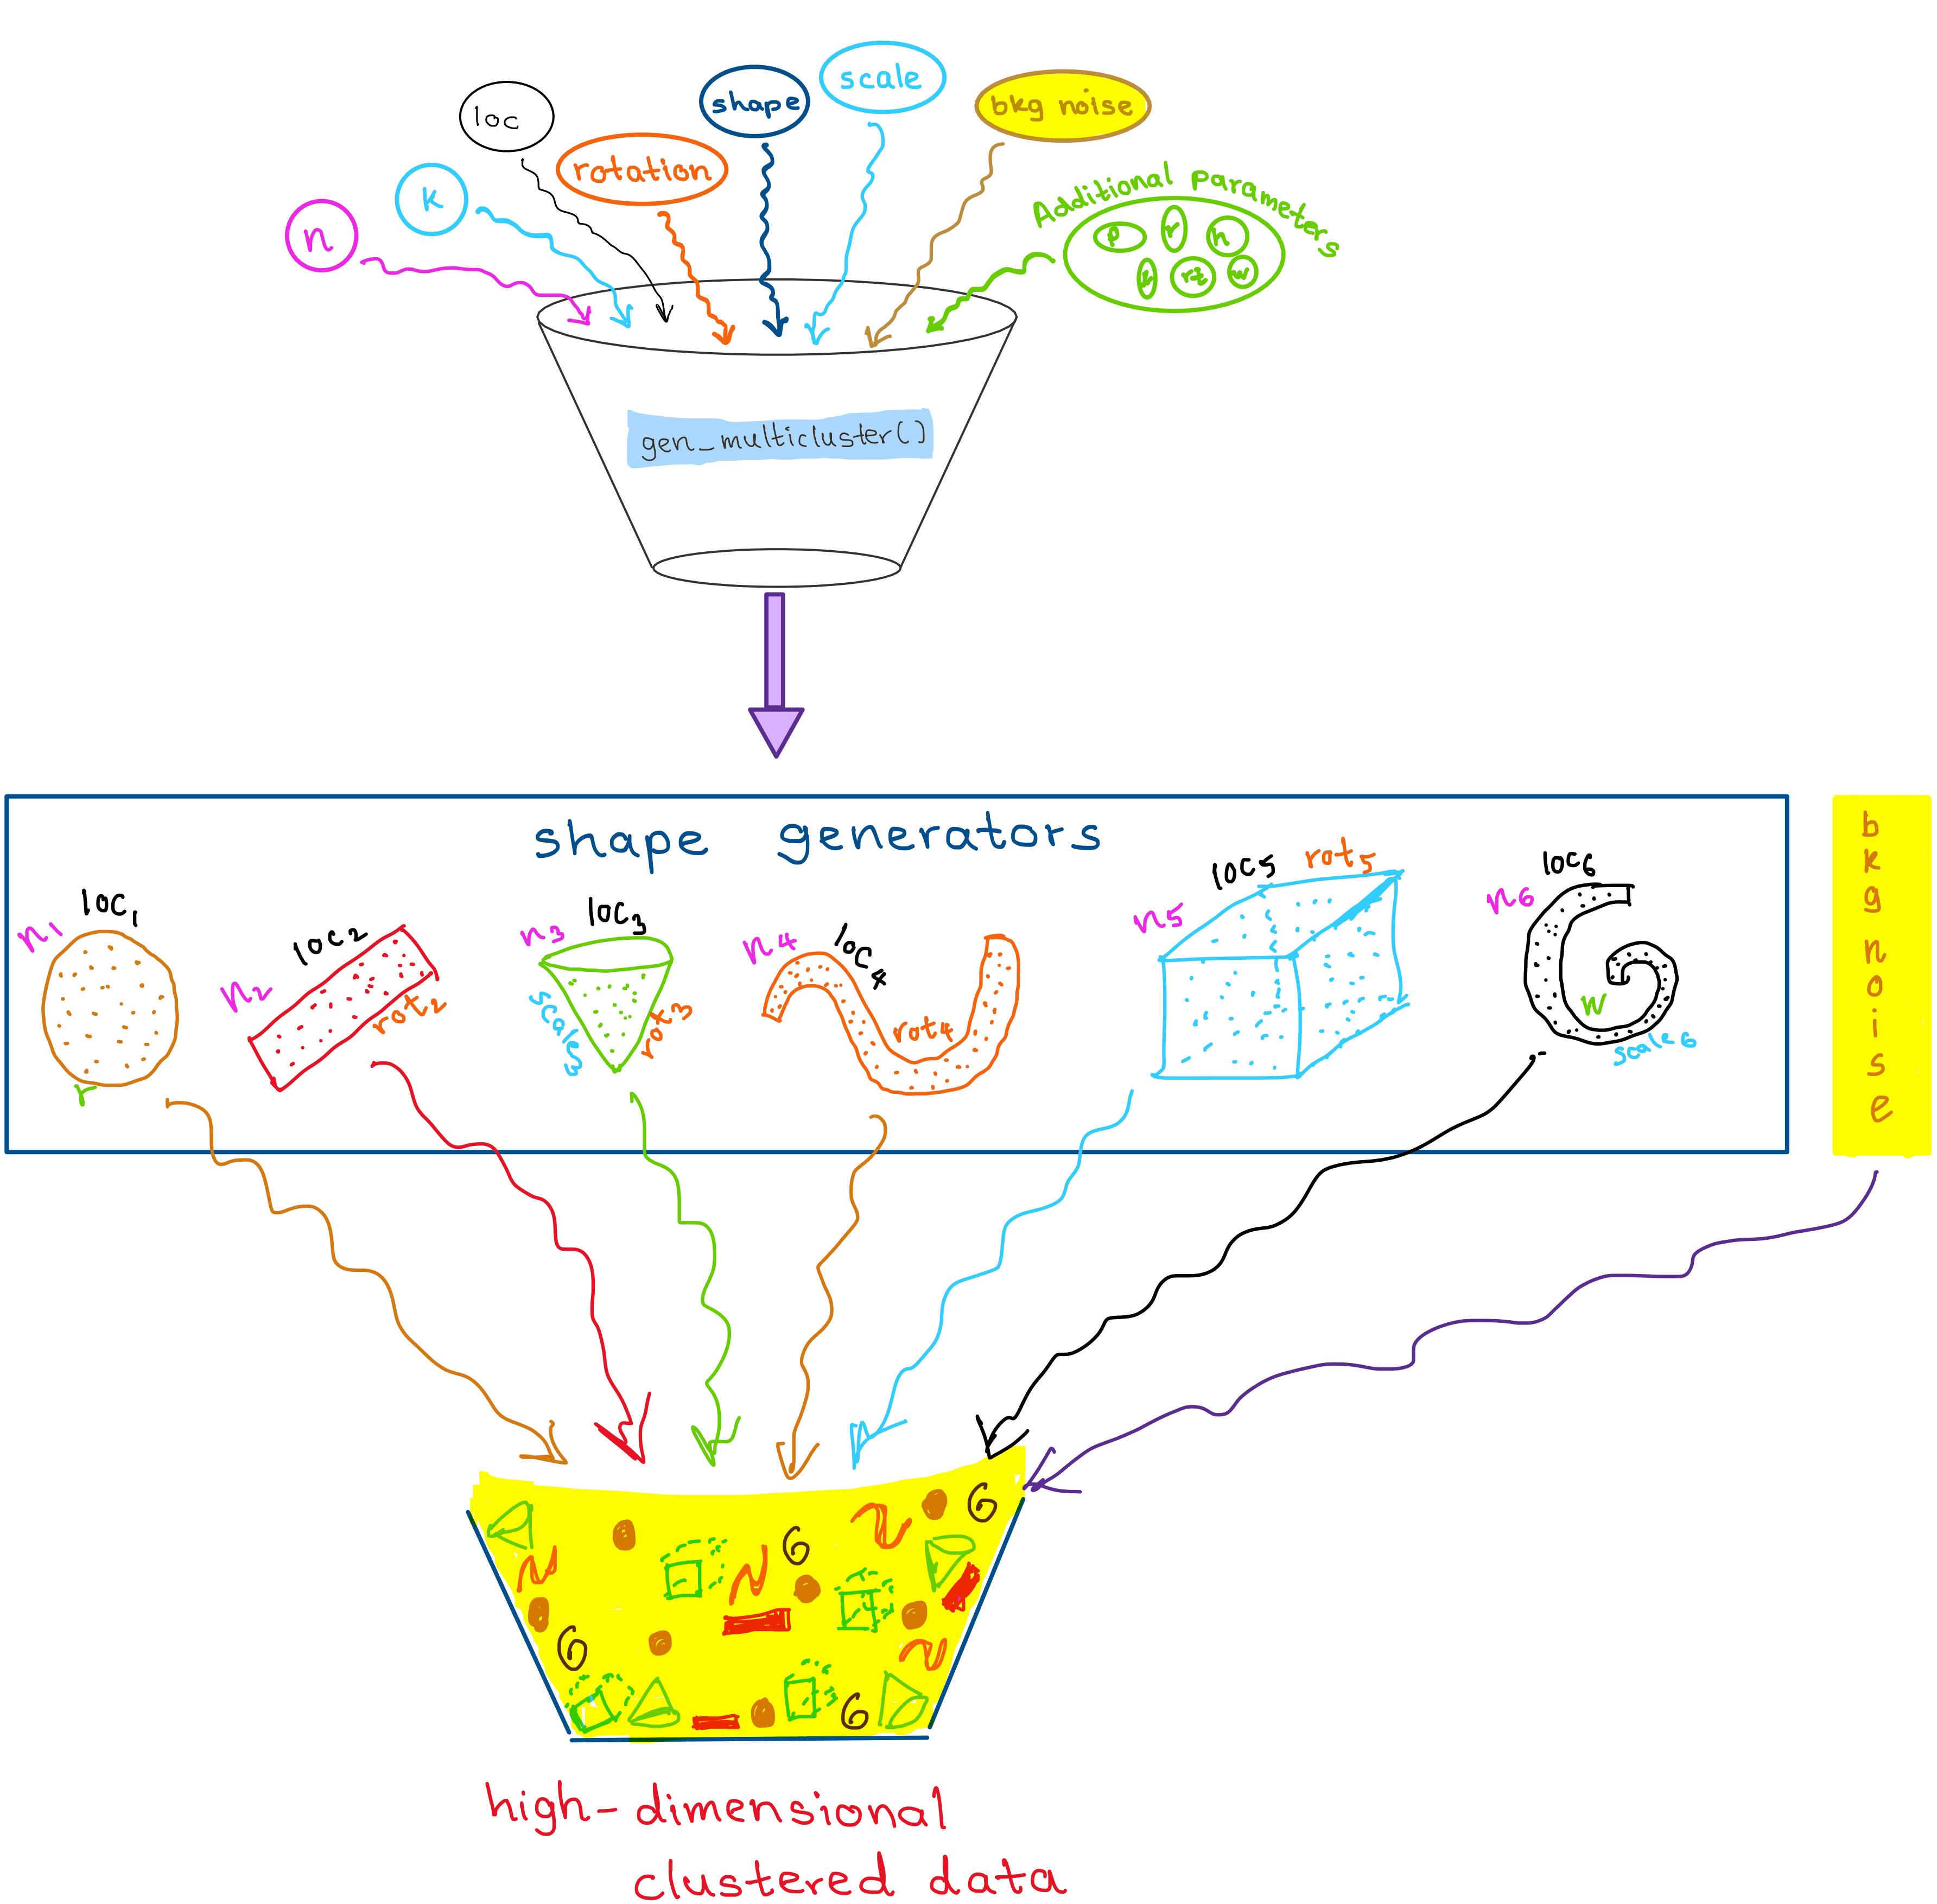
\includegraphics[width=1\linewidth,height=\textheight,keepaspectratio]{chapters/../figures/cardinalR/cardinalR_workflow.png}

}

\caption{Workflow for generating high-dimensional clustered data. The
user specifies input parameters (number of points, clusters, cluster
shapes, scaling, rotation, and optional background noise). Clusters are
generated iteratively, transformed, optionally augmented with Gaussian
noise dimensions, combined, and labeled, resulting in the final
dataset.}

\end{figure}%

\section{Usage}\label{usage-1}

The \texttt{cardinalR} R package is available on GitHub at
\href{https://github.com/JayaniLakshika/cardinalR}{JayaniLakshika/cardinalR}.

\subsection{Main function}\label{main-function-1}

The main function of the package is \texttt{gen\_multicluster()}, which
generates datasets consisting of multiple clusters with user-specified
characteristics. Users can control the number of clusters (\texttt{k}),
and the number of points in each cluster (\texttt{n}). Each cluster can
take on a different geometric shape (e.g., Gaussian, cone, uniform cube)
by specifying the corresponding generator function (\texttt{shape}), can
be scaled to adjust its spread, rotated using custom rotation matrices
(\texttt{rotation}), and positioned at defined centroids (\texttt{loc}).
The function ensures flexibility in cluster location and orientation,
allowing users to simulate complex high-dimensional structures.

To maintain consistency across generators, the function identifies the
arguments required by each chosen generator function and supplies only
those arguments that are valid for that specific generator. This design
enables the combination of cluster types with differing parameter
requirements within the same dataset. When clusters are generated with
fewer dimensions than others, the function augments the
lower-dimensional clusters with additional Gaussian noise variables so
that all clusters are represented in the same dimensional space. These
noise dimensions are drawn independently from normal distributions

\[
X \sim \mathcal{N}(m, s^2),
\]

where the mean (\(m\)) is set to the average of the cluster coordinates
and the standard deviation (\(s\)) defaults to \(0.2\).

An optional argument, \texttt{is\_bkg}, adds background noise drawn from
a multivariate normal distribution centered on the dataset's overall
mean with standard deviations matching the observed spread. Extra
arguments (\texttt{...}) can be passed to cluster generators, allowing
further control over per-cluster characteristics like radius of the
sphere. The main arguments of the \texttt{gen\_multicluster()} function
are shown in Table @ref(tab:main-tb-pdf).

\begin{table}

\caption{\label{tab:main-tb-pdf}The main arguments for gen\_multicluster().}
\centering
\begin{tabular}[t]{>{\raggedright\arraybackslash}p{2cm}>{\raggedright\arraybackslash}p{3cm}>{\raggedright\arraybackslash}p{8cm}}
\toprule
Argument & Type & Explanation\\
\midrule
n & numeric (vector) & Number of points in each cluster.\\
k & numeric & Number of clusters.\\
loc & numeric (matrix) & Locations/centroids of clusters.\\
scale & numeric (vector) & Scaling factors of clusters.\\
shape & character (vector) & Shapes of clusters.\\
rotation & numeric (list) & Rotation matrices, one per cluster.\\
is\_bkg & boolean & Background noise should exist or not.\\
\bottomrule
\end{tabular}
\end{table}

The following example demonstrates how to use
\texttt{gen\_multicluster()} to create a \(4\text{-}D\) dataset with
three clusters of different shapes and orientations:

\begin{Shaded}
\begin{Highlighting}[]
\CommentTok{\# Define example rotation matrices for 4D space}
\NormalTok{rot1 }\OtherTok{\textless{}{-}} \FunctionTok{gen\_rotation}\NormalTok{(}\AttributeTok{p =} \DecValTok{4}\NormalTok{, }\AttributeTok{planes\_angles =} \FunctionTok{list}\NormalTok{(}
  \FunctionTok{list}\NormalTok{(}\AttributeTok{plane =} \FunctionTok{c}\NormalTok{(}\DecValTok{1}\NormalTok{, }\DecValTok{2}\NormalTok{), }\AttributeTok{angle =} \DecValTok{60}\NormalTok{),}
  \FunctionTok{list}\NormalTok{(}\AttributeTok{plane =} \FunctionTok{c}\NormalTok{(}\DecValTok{3}\NormalTok{, }\DecValTok{4}\NormalTok{), }\AttributeTok{angle =} \DecValTok{90}\NormalTok{)}
\NormalTok{))}

\NormalTok{rot2 }\OtherTok{\textless{}{-}} \FunctionTok{gen\_rotation}\NormalTok{(}\AttributeTok{p =} \DecValTok{4}\NormalTok{, }\AttributeTok{planes\_angles =} \FunctionTok{list}\NormalTok{(}
  \FunctionTok{list}\NormalTok{(}\AttributeTok{plane =} \FunctionTok{c}\NormalTok{(}\DecValTok{1}\NormalTok{, }\DecValTok{3}\NormalTok{), }\AttributeTok{angle =} \DecValTok{30}\NormalTok{)}
\NormalTok{))}

\NormalTok{rot3 }\OtherTok{\textless{}{-}} \FunctionTok{gen\_rotation}\NormalTok{(}\AttributeTok{p =} \DecValTok{4}\NormalTok{, }\AttributeTok{planes\_angles =} \FunctionTok{list}\NormalTok{(}
  \FunctionTok{list}\NormalTok{(}\AttributeTok{plane =} \FunctionTok{c}\NormalTok{(}\DecValTok{2}\NormalTok{, }\DecValTok{4}\NormalTok{), }\AttributeTok{angle =} \DecValTok{45}\NormalTok{)}
\NormalTok{))}

\CommentTok{\# Generate the clustered dataset}
\NormalTok{clust\_data }\OtherTok{\textless{}{-}} \FunctionTok{gen\_multicluster}\NormalTok{(}
  \AttributeTok{n =} \FunctionTok{c}\NormalTok{(}\DecValTok{200}\NormalTok{, }\DecValTok{300}\NormalTok{, }\DecValTok{500}\NormalTok{),}
  \AttributeTok{k =} \DecValTok{3}\NormalTok{,}
  \AttributeTok{loc =} \FunctionTok{matrix}\NormalTok{(}\FunctionTok{c}\NormalTok{(}
    \DecValTok{0}\NormalTok{, }\DecValTok{0}\NormalTok{, }\DecValTok{0}\NormalTok{, }\DecValTok{0}\NormalTok{,}
    \DecValTok{5}\NormalTok{, }\DecValTok{9}\NormalTok{, }\DecValTok{0}\NormalTok{, }\DecValTok{0}\NormalTok{,}
    \DecValTok{3}\NormalTok{, }\DecValTok{4}\NormalTok{, }\DecValTok{10}\NormalTok{, }\DecValTok{7}
\NormalTok{  ), }\AttributeTok{nrow =} \DecValTok{3}\NormalTok{, }\AttributeTok{byrow =} \ConstantTok{TRUE}\NormalTok{),}
  \AttributeTok{scale =} \FunctionTok{c}\NormalTok{(}\DecValTok{3}\NormalTok{, }\DecValTok{1}\NormalTok{, }\DecValTok{2}\NormalTok{),}
  \AttributeTok{shape =} \FunctionTok{c}\NormalTok{(}\StringTok{"gaussian"}\NormalTok{, }\StringTok{"cone"}\NormalTok{, }\StringTok{"unifcube"}\NormalTok{),}
  \AttributeTok{rotation =} \FunctionTok{list}\NormalTok{(rot1, rot2, rot3),}
  \AttributeTok{is\_bkg =} \ConstantTok{FALSE}
\NormalTok{)}
\end{Highlighting}
\end{Shaded}

\subsection{Shape generators}\label{shape-generators}

The shape generators form the foundation of the package, providing
functions to create synthetic datasets from simple, well-defined
geometric forms such as cones, pyramids, spheres, grids, and branching
structures. Each generator includes the parameter \texttt{n}, which
specifies the number of points to generate. Some functions, such as
\texttt{gen\_unifcube()}, also take the dimension \texttt{p}, while
others include arguments specific to the geometry (e.g., radius for
spheres (\texttt{r}), width for bands (\texttt{w})). If
higher-dimensional data are required, additional noise dimensions can be
appended after data generation using any noise generator function. This
flexibility allows users to construct both low- and high-dimensional
datasets from the same underlying structures.

\subsubsection{Branching}\label{branching}

A branching structure (Figure @ref(fig:branch-proj)) captures
trajectories that diverge or bifurcate from a common origin, similar to
processes such as cell differentiation in biology
((\citeproc{ref-trapnell2014}{\textbf{trapnell2014?}})). We introduce a
set of data generation functions specifically designed to simulate
high-dimensional branching structures with various geometries, numbers
of points (\texttt{n}), and number of branches (\texttt{k}). Although
these functions can generate multiple branches, they do not produce a
formal \emph{multicluster} dataset: the branches form a single connected
structure, with multiple visually distinct arms rather than independent
clusters. Table @ref(tab:branching-tb-pdf) outlines these functions. The
main arguments of the functions described in Table
@ref(tab:arg-branching-tb-pdf).

\begin{table}

\caption{\label{tab:branching-tb-pdf}cardinalR branching data generation functions}
\centering
\begin{tabular}[t]{>{\raggedright\arraybackslash}p{4cm}>{\raggedright\arraybackslash}p{8cm}}
\toprule
Function & Explanation\\
\midrule
gen\_expbranches & Exponential shaped branches.\\
gen\_linearbranches & Linear shaped branches.\\
gen\_curvybranches & Curvy shaped branches.\\
gen\_orglinearbranches & Linear shaped branches originated in one point.\\
gen\_orgcurvybranches & Curvy shaped branches originated in one point.\\
\bottomrule
\end{tabular}
\end{table}

\begin{table}

\caption{\label{tab:arg-branching-tb-pdf}The main arguments for branching shape generators.}
\centering
\begin{tabular}[t]{>{\raggedright\arraybackslash}p{2cm}>{\raggedright\arraybackslash}p{3cm}l}
\toprule
Argument & Type & Explanation\\
\midrule
n & integer & Number of points.\\
k & integer & Number of clusters.\\
\bottomrule
\end{tabular}
\end{table}

The simplest structures are approximately linear branches in \gD{},
generated by the \texttt{gen\_linearbranches(n,\ k)} function. These
consist of \(k\) short line segments in the first two dimensions, with
added jitter to simulate variability. Mathematically, each branch \(i\)
is defined as

\[
X_1 \sim U(a_i, b_i), \quad X_2 = s_i (X_1 - x_{\text{start},i}) + y_{\text{start},i} + \epsilon, \quad \epsilon \sim U(0, \delta),
\]

where \((x_{\text{start},i}, y_{\text{start},i})\) is the starting point
of branch \(i\), \(\delta\) controls local jitter, and \(s_i\) is the
slope, initialized as

\[
s_i =
\begin{cases}
0.5 & i = 1, \\
-0.5 & i = 2, \\
\text{randomly sampled from } [s_{\min}, s_{\max}] & i = 3, \dots, k.
\end{cases}
\]

Branches \(1\) and \(2\) are initialized with fixed slopes and
intercepts, while later branches are iteratively added at locations
chosen to avoid overlap with existing branches, producing a set of
connected linear paths.

\begin{Shaded}
\begin{Highlighting}[]
\NormalTok{linearbranches }\OtherTok{\textless{}{-}} \FunctionTok{gen\_linearbranches}\NormalTok{(}\AttributeTok{n =} \DecValTok{1000}\NormalTok{, }\AttributeTok{k =} \DecValTok{4}\NormalTok{)}
\end{Highlighting}
\end{Shaded}

To introduce curvature, the \texttt{gen\_curvybranches(n,\ k)} function
generates \(k\) curvilinear branches in \gD{}. Branches \(1\) and \(2\)
are simple parabolas defined as

\[
\begin{aligned}
\text{Branch 1: } & X_1 \sim U(0,1), \quad X_2 = 0.1 X_1 + X_1^2 + \epsilon, \\
\text{Branch 2: } & X_1 \sim U(-1,0), \quad X_2 = 0.1 X_1 - 2 X_1^2 + \epsilon, \quad \epsilon \sim U(0, \delta),
\end{aligned}
\]

where \(\delta\) controls local jitter. Additional branches are attached
iteratively to existing structures. Each new branch \(i\) starts at a
selected point \((x_{\text{start},i}, y_{\text{start},i})\) from the
current structure and extends according to

\[
X_1 \sim U(x_{\text{start},i}, x_{\text{start},i}+1), \quad X_2 = 0.1 X_1 - s_i (X_1^2 - x_{\text{start},i}) + y_{\text{start},i},
\]

where \(s_i\) is a scale factor controlling the curvature of branch
\(i\). For the first few initial branches, \(s_i\) can be fixed (e.g.,
\(s_1 = 1, s_2 = 2\)), while for subsequent branches it is sampled from
a predefined set, such as
\(s_i \in \{-2, -1.5, -1, -0.5, 0, 0.5, 1, 1.5\}\), to create
variability in curvature.

\begin{Shaded}
\begin{Highlighting}[]
\NormalTok{curvybranches }\OtherTok{\textless{}{-}} \FunctionTok{gen\_curvybranches}\NormalTok{(}\AttributeTok{n =} \DecValTok{1000}\NormalTok{, }\AttributeTok{k =} \DecValTok{4}\NormalTok{)}
\end{Highlighting}
\end{Shaded}

The \texttt{gen\_expbranches(n,\ k)} function creates \(k\) exponential
branches in \gD{}, radiating from a central region. Each branch \(i\) is
defined as

\[
X_1 \sim U(-2,2), \quad X_2 = \exp(\sigma_i \, s_i \, X_1) + \epsilon, \quad \epsilon \sim U(0, \delta), \quad s_i \sim U(0.5,2),
\]

where \(\sigma_i = (-1)^{i+1}\) alternates the sign of the exponent to
produce mirror-symmetric branches. The parameter \(s_i\) controls the
steepness of branch \(i\), and \(\delta\) introduces small local jitter.

\begin{Shaded}
\begin{Highlighting}[]
\NormalTok{expbranches }\OtherTok{\textless{}{-}} \FunctionTok{gen\_expbranches}\NormalTok{(}\AttributeTok{n =} \DecValTok{1000}\NormalTok{, }\AttributeTok{k =} \DecValTok{4}\NormalTok{)}
\end{Highlighting}
\end{Shaded}

High-dimensional generalizations are provided by
\texttt{gen\_orglinearbranches(n,\ p,\ k)} (Figure
@ref(fig:branch-proj)) and \texttt{gen\_orgcurvybranches(n,\ p,\ k)}.
Each branch is embedded in a unique or repeated \(2\text{-}D\) subspace
of the \(p\text{-}D\) space. When \texttt{allow\_share\ =\ TRUE},
multiple branches may share the same subspace; otherwise, subspaces are
sampled without replacement until all possible \(\binom{p}{2}\)
combinations are exhausted, after which additional branches may repeat
subspaces. Linear branches follow

\[
X_{i_1} \sim U(a_i,b_i), \quad X_{i_2} = s_i X_{i_1} + \epsilon, \quad \epsilon \sim N(0, \sigma^2),
\]

while curvilinear branches include a quadratic term

\[
X_{i_1} \sim U(a_i,b_i), \quad X_{i_2} = - s_i X_{i_1}^2 + \epsilon, \quad \epsilon \sim N(0, \sigma^2),
\]

where \(a_i, b_i\) define the range of the first coordinate for branch
\(i\), and \(\epsilon\) is Gaussian noise added to introduce
variability. The scale factor \(s_i\) controls slope (linear branches)
or curvature (curvilinear branches) and is assigned as follows: for the
first \(\binom{p}{2}\) branches, \(s_i = 1\); for additional branches
when \(k > \binom{p}{2}\), \(s_i\) is randomly drawn from the set
\(\{1, 1.5, 2, \dots, 8\}\).

\begin{Shaded}
\begin{Highlighting}[]
\NormalTok{orglinearbranches }\OtherTok{\textless{}{-}} \FunctionTok{gen\_orglinearbranches}\NormalTok{(}\AttributeTok{n =} \DecValTok{1000}\NormalTok{, }\AttributeTok{p =} \DecValTok{4}\NormalTok{, }\AttributeTok{k =} \DecValTok{4}\NormalTok{)}
\end{Highlighting}
\end{Shaded}

\begin{Shaded}
\begin{Highlighting}[]
\NormalTok{orgcurvybranches }\OtherTok{\textless{}{-}} \FunctionTok{gen\_orgcurvybranches}\NormalTok{(}\AttributeTok{n =} \DecValTok{1000}\NormalTok{, }\AttributeTok{p =} \DecValTok{4}\NormalTok{, }\AttributeTok{k =} \DecValTok{4}\NormalTok{)}
\end{Highlighting}
\end{Shaded}

\begin{figure}[H]

{\centering 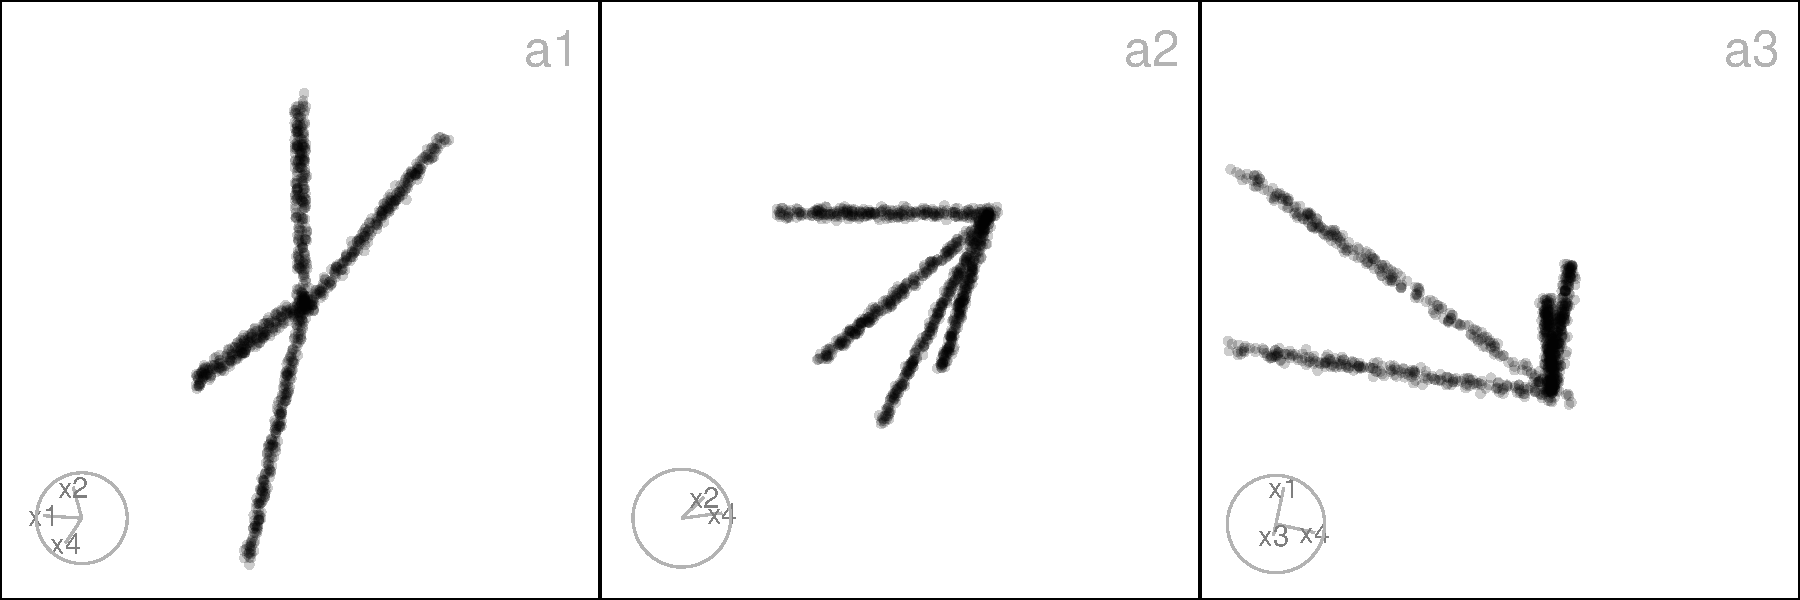
\includegraphics[width=1\linewidth,height=\textheight,keepaspectratio]{chapters/04-chap4_files/figure-pdf/branch-proj-1.pdf}

}

\caption{Three \(2\text{-}D\) projections from the \(4\text{-}D\)
\texttt{orglinearbranches} data. Each shows a different projection,
illustrating how the linear branches appear from multiple viewing
angles. These views highlight the dataset's underlying branching
structure and demonstrate how projections reveal patterns that are
otherwise hidden in higher dimensions.}

\end{figure}%

\subsubsection{Cone}\label{cone}

To simulate a cone-shaped structure in arbitrary dimensions (Figure
@ref(fig:cone-proj)), we define a function
\texttt{gen\_cone(n,\ p,\ h,\ ratio)}, which creates a high-dimensional
cone with options for a sharp or blunted apex, allowing for a dense
concentration of points near the tip.

This function generates \(n\) points in \(p\text{-}D\), where the last
dimension, \(X_p\), represents the height along the cone's axis, and the
first \(p-1\) dimensions define a shrinking hyperspherical cross-section
toward the tip. Heights are sampled from a truncated exponential
distribution, \(X_p \sim \text{Exp}(\lambda = 2/h)\), capped at the cone
height \(h\), producing a higher density of points near the tip. At each
height \(X_p\), the radius of the cross-section decreases linearly from
base to tip according to
\(r = r_{\text{min}} + (r_{\text{max}} - r_{\text{min}}) X_p / h\),
where \(r_{\text{min}} = \text{ratio}\) and \(r_{\text{max}} = 1\).

For each point, a direction in the first \(p-1\) dimensions is sampled
uniformly on a \((p-1)\)-dimensional hypersphere using generalized
spherical coordinates. The radial coordinates are scaled by the
height-dependent radius \(r\), producing the conical taper. In three
dimensions (\(p = 3\)), this results in a classical \(3\text{-}D\) cone,
while for \(p > 3\), additional dimensions provide a smooth embedding
into higher-dimensional space, preserving the conical structure.

\begin{Shaded}
\begin{Highlighting}[]
\NormalTok{cone }\OtherTok{\textless{}{-}} \FunctionTok{gen\_cone}\NormalTok{(}\AttributeTok{n =} \DecValTok{1000}\NormalTok{, }\AttributeTok{p =} \DecValTok{4}\NormalTok{, }\AttributeTok{h =} \DecValTok{5}\NormalTok{, }\AttributeTok{ratio =} \FloatTok{0.5}\NormalTok{)}
\end{Highlighting}
\end{Shaded}

Cone-shaped structures appear in particle dispersions, light beams, and
tapering processes, where spread decreases along one axis. They are also
used to benchmark clustering and dimensionality reduction methods
(\citeproc{ref-hadsell2006}{\textbf{hadsell2006?}}).

\begin{figure}[H]

{\centering 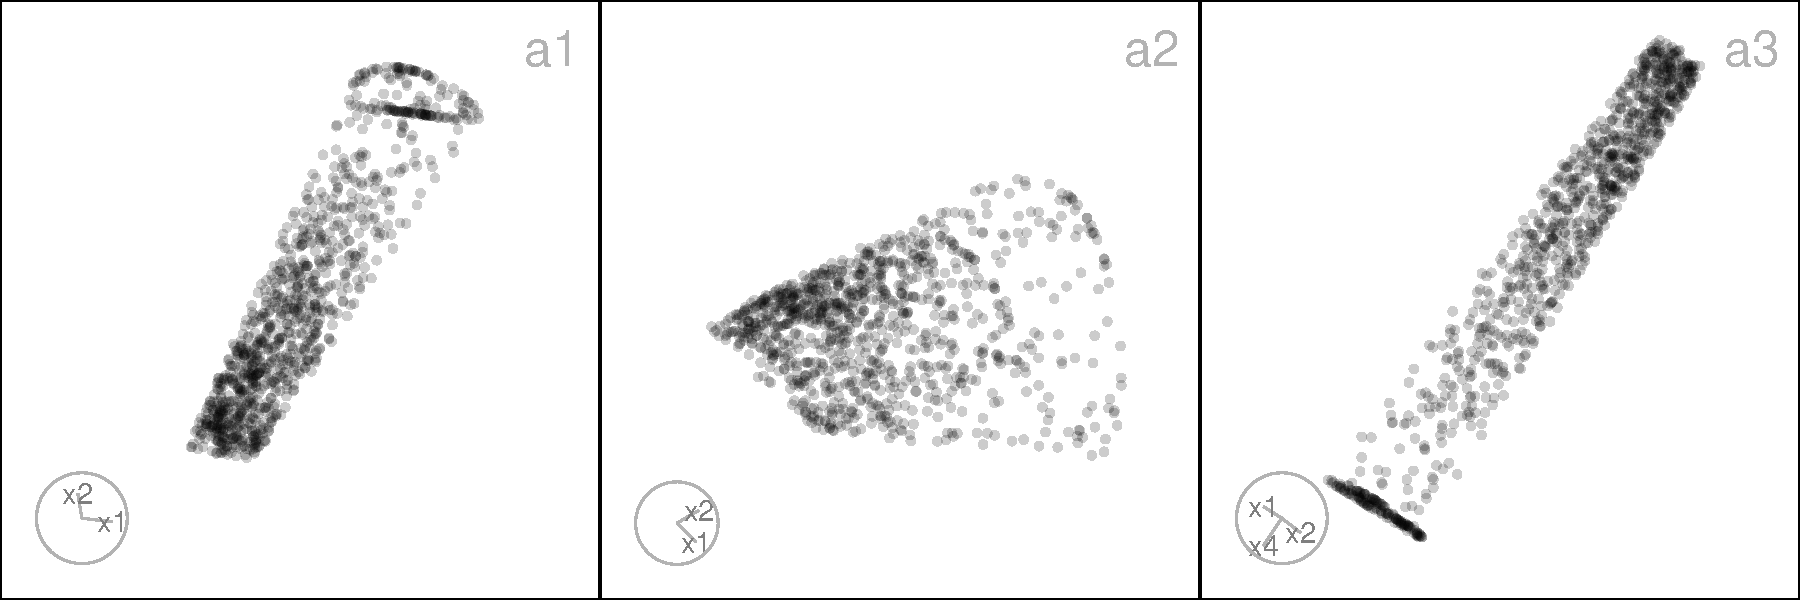
\includegraphics[width=1\linewidth,height=\textheight,keepaspectratio]{chapters/04-chap4_files/figure-pdf/cone-proj-1.pdf}

}

\caption{Three \(2\text{-}D\) projections from the \(3\text{-}D\)
\texttt{cone} data. Points are concentrated near the tip along the
height dimension, while the radius of the hyperspherical cross-section
decreases linearly toward the apex. These projections show how the
conical geometry is preserved.}

\end{figure}%

\subsubsection{Cube}\label{cube}

A cube structure represents uniformly or systematically distributed
points within a high-dimensional hypercube, providing a useful framework
for assessing how well algorithms preserve uniformity, and boundary
properties in high dimensions. We provide a set of functions to generate
high-dimensional cube structures with flexible configurations, including
regular grids, and uniform random points. Table @ref(tab:cube-tb-pdf)
outlines these functions and their purposes.

\begin{table}

\caption{\label{tab:cube-tb-pdf}cardinalR cube data generation functions}
\centering
\begin{tabular}[t]{>{\raggedright\arraybackslash}p{4cm}>{\raggedright\arraybackslash}p{8cm}}
\toprule
Function & Explanation\\
\midrule
gen\_gridcube & Cube with specified grid points along each axes.\\
gen\_unifcube & Cube with uniform points.\\
\bottomrule
\end{tabular}
\end{table}

The function \texttt{gen\_gridcube(n,\ p)} is a wrapper around
\texttt{geozoo::cube.solid.grid()}. It generates a regular lattice of
points in \pD{}, producing a uniform hypercube grid. Each axis contains
equally spaced coordinates, resulting in a well-defined geometric
structure.

\begin{Shaded}
\begin{Highlighting}[]
\NormalTok{gridcube }\OtherTok{\textless{}{-}} \FunctionTok{gen\_gridcube}\NormalTok{(}\AttributeTok{n =} \DecValTok{1000}\NormalTok{, }\AttributeTok{p =} \DecValTok{4}\NormalTok{)}
\end{Highlighting}
\end{Shaded}

By contrast, \texttt{gen\_unifcube(n,\ p)} wraps
\texttt{geozoo::cube.solid.random()}, producing uniformly distributed
points within a \(p\text{-}D\) cube. To avoid including the cube's
vertices, these points are removed after generation. This results in a
hypercube filled with random, but evenly distributed, samples rather
than structured lattice points.

\begin{Shaded}
\begin{Highlighting}[]
\NormalTok{unifcube }\OtherTok{\textless{}{-}} \FunctionTok{gen\_unifcube}\NormalTok{(}\AttributeTok{n =} \DecValTok{1000}\NormalTok{, }\AttributeTok{p =} \DecValTok{4}\NormalTok{)}
\end{Highlighting}
\end{Shaded}

Such cube-based structures are commonly used as benchmarks in Monte
Carlo sampling, computational geometry, and density estimation, where
assessing how algorithms behave under uniform or grid-like distributions
is critical (\citeproc{ref-devroye1986}{\textbf{devroye1986?}};
\citeproc{ref-niederreiter1992}{\textbf{niederreiter1992?}}).

\subsubsection{Gaussian}\label{gaussian}

The \texttt{gen\_gaussian(n,\ p,\ s)} function generates a multivariate
Gaussian cloud in \(p\text{-}D\), centered at the origin with
user-defined covariance structure. Each point is independently drawn
using the multivariate normal distribution with
\(X_i \sim N_p(\boldsymbol{0}, s)\), where \(s\) is a user-defined
\(p \times p\) positive-definite matrix.

\begin{Shaded}
\begin{Highlighting}[]
\NormalTok{gau }\OtherTok{\textless{}{-}} \FunctionTok{gen\_gaussian}\NormalTok{(}\AttributeTok{n =} \DecValTok{1000}\NormalTok{, }\AttributeTok{p =} \DecValTok{4}\NormalTok{, }\AttributeTok{s =} \FunctionTok{diag}\NormalTok{(}\DecValTok{4}\NormalTok{))}
\end{Highlighting}
\end{Shaded}

Gaussian clouds are common benchmark structures in statistics and
machine learning, used in clustering, classification, and anomaly
detection, with applications in image segmentation, speech recognition,
and forensic analysis
(\citeproc{ref-geoffrey2000}{\textbf{geoffrey2000?}}).

\subsubsection{Linear}\label{linear}

The \texttt{gen\_longlinear(n,\ p)} function generates a
high-dimensional dataset representing a long linear structure with
noise. Each variable is formed as
\(X_i = \text{scale}_i \cdot (0,1,\dots,n{-}1 + \epsilon) + \text{shift}_i\),
where \(\text{scale}\_i \sim U(-10, 10)\) determines the orientation of
the line in each dimension, \(\text{shift}\_i \sim U(-300, 300)\)
offsets the line to separate dimensions, and
\(\epsilon \sim N(0, (0.03n)^2)\) introduces Gaussian noise.

\begin{Shaded}
\begin{Highlighting}[]
\NormalTok{linear }\OtherTok{\textless{}{-}} \FunctionTok{gen\_longlinear}\NormalTok{(}\AttributeTok{n =} \DecValTok{1000}\NormalTok{, }\AttributeTok{p =} \DecValTok{4}\NormalTok{)}
\end{Highlighting}
\end{Shaded}

This structure appears in \pD{} data when variation is driven by a
single factor, such as time-course or sensor measurements, providing a
useful test case for trajectory and regression methods
(\citeproc{ref-trapnell2014}{\textbf{trapnell2014?}}).

\subsubsection{Möbius}\label{muxf6bius}

The \texttt{gen\_mobius()} function is a wrapper around
\texttt{geozoo::mobius()}, designed to simplify the generation of a
Möbius strip in three dimensions for use in high-dimensional diagnostic
studies. The function returns a tibble with \(n\) sampled points forming
the surface of a Möbius strip.

\begin{Shaded}
\begin{Highlighting}[]
\NormalTok{mobius }\OtherTok{\textless{}{-}} \FunctionTok{gen\_mobius}\NormalTok{(}\AttributeTok{n =} \DecValTok{1000}\NormalTok{)}
\end{Highlighting}
\end{Shaded}

The Möbius strip structure can model twisted or cyclic surfaces in
physics and engineering, such as conveyor belts, molecular structures,
or optical systems with non-orientable geometries
(\citeproc{ref-optica2023}{\textbf{optica2023?}}).

\subsubsection{Polynomial}\label{polynomial}

A polynomial structure generates data points that follow non-linear
curvilinear relationships, such as quadratic or cubic trends, in \gD{}
space. To extend these patterns into high-dimensional settings,
additional noise dimensions can be added. These patterns are useful for
evaluating how well algorithms capture smooth, non-linear trajectories
and curvature in the data. We provide functions for generating quadratic
and cubic structures, enabling controlled experiments with different
degrees of polynomial complexity. Table @ref(tab:polynomial-tb-pdf)
summarizes these functions and their purposes.

\begin{table}

\caption{\label{tab:polynomial-tb-pdf}cardinalR polynomial data generation functions}
\centering
\begin{tabular}[t]{>{\raggedright\arraybackslash}p{4cm}>{\raggedright\arraybackslash}p{8cm}}
\toprule
Function & Explanation\\
\midrule
gen\_quadratic & Quadratic pattern.\\
gen\_cubic & Cubic pattern.\\
\bottomrule
\end{tabular}
\end{table}

The first is the quadratic curve of \(n\) points in two dimensions. This
is generated using \texttt{gen\_quadratic(n,\ range)}. The independent
variable is defined as \(X_1 \sim U(\text{range}[1], \text{range}[2])\),
and a raw polynomial basis of degree 2 is applied to form
\(X_2 = X_1 - X_1^2 + \varepsilon_2\), where
\(\varepsilon_2 \sim U(0, 0.5)\). This produces a smooth parabolic arc
opening downward, with vertical jitter introduced by the noise term.

\begin{Shaded}
\begin{Highlighting}[]
\NormalTok{quadratic }\OtherTok{\textless{}{-}} \FunctionTok{gen\_quadratic}\NormalTok{(}\AttributeTok{n =} \DecValTok{1000}\NormalTok{)}
\end{Highlighting}
\end{Shaded}

The second is the cubic curve of \(n\) points in two dimensions. This is
generated using \texttt{gen\_cubic(n,\ range)}. The independent variable
is defined as \(X_1 \sim U(\text{range}[1], \text{range}[2])\), and a
raw polynomial basis of degree \(3\) is applied to construct
\(X_2 = X_1 + X_1^2 - X_1^3 + \varepsilon_2\), where
\(\varepsilon_2 \sim U(0, 0.5)\). This produces a more complex
curvilinear structure than the quadratic case, with both upward and
downward turning points.

\begin{Shaded}
\begin{Highlighting}[]
\NormalTok{cubic }\OtherTok{\textless{}{-}} \FunctionTok{gen\_cubic}\NormalTok{(}\AttributeTok{n =} \DecValTok{1000}\NormalTok{)}
\end{Highlighting}
\end{Shaded}

\subsubsection{Pyramid}\label{pyramid}

A pyramid structure (Figure @ref(fig:pyr-proj)) represents data arranged
around a central apex and base, useful for exploring how algorithms
handle pointed or layered geometries in \pD{} space. The functions
provided allow users to generate pyramids with rectangular, triangular,
and star-shaped bases, and sharp or blunted apexes. Additionally, it is
possible to create a pyramid with a fractal-like internal structure,
enabling the study of non-convex and sparse regions. Table
@ref(tab:pyramid-tb-pdf) summarizes these functions.

\begin{table}

\caption{\label{tab:pyramid-tb-pdf}cardinalR pyramid data generation functions}
\centering
\begin{tabular}[t]{>{\raggedright\arraybackslash}p{4cm}>{\raggedright\arraybackslash}p{8cm}}
\toprule
Function & Explanation\\
\midrule
gen\_pyrrect & Rectangular-base, with a sharp or blunted apex.\\
gen\_pyrtri & Triangular-base, with a sharp or blunted apex.\\
gen\_pyrstar & Star-shaped base, with a sharp or blunted apex.\\
gen\_pyrfrac & Pyramid with triangular pyramid-shaped holes.\\
\bottomrule
\end{tabular}
\end{table}

Let \(X_1, \dots, X_p\) denote the coordinates of the generated points.
For the rectangular, triangular, and star-shaped based pyramid generator
functions, the final dimension, \(X_p\), encodes the height of each
point and is drawn from an exponential distribution capped at the
maximum height \(h\). That is,
\(X_p = z \sim \min\left(\text{Exp}(\lambda = 2/h),\ h\right).\) This
distribution creates a natural skew toward smaller height values,
resulting in a denser concentration of points near the pyramid's apex.
For the star-shaped base pyramid, the final dimension is drawn from a
uniform distribution. That is, \(X_p = z \sim U(0, h)\).

The remaining dimensions are based on the specific pyramid shape. For
the rectangular based pyramid,
\texttt{gen\_pyrrect(n,\ p,\ h,\ l\_vec,\ rt)} (Figure
@ref(fig:pyr-proj) a), let \(r_x(z)\) and \(r_y(z)\) denote the
half-widths of the rectangular cross-section at height \(z\). That is,
\(r_x(z) = r_t + (l_x - r_t)z/h\), \(r_y(z) = r_t + (l_y - r_t)z/h\).
The first three coordinates are then defined as
\(X_1 \sim U(-r_x(z),\ r_x(z)), \quad X_2 \sim U(-r_y(z),\ r_y(z)),\text{ and }X_3 \sim U(-r_x(z),\ r_x(z)).\)

\begin{Shaded}
\begin{Highlighting}[]
\NormalTok{pyrrect }\OtherTok{\textless{}{-}} \FunctionTok{gen\_pyrrect}\NormalTok{(}\AttributeTok{n =} \DecValTok{1000}\NormalTok{, }\AttributeTok{p =} \DecValTok{4}\NormalTok{)}
\end{Highlighting}
\end{Shaded}

For the triangular based pyramid,
\texttt{gen\_pyrtri(n,\ p,\ h,\ l,\ rt)} (Figure @ref(fig:pyr-proj) b),
let \(r(z)\) denote the scaling factor (distance from the origin to
triangle vertices) at height \(z\). That is,
\(r(z) = r_t + (l-r_t)z/h\). A point in the triangle at height \(z\) is
generated using barycentric coordinates \((u, v)\) to ensure uniform
sampling within the triangular cross-section:
\(u, v \sim U(0, 1), \quad \text{if } u + v > 1: u \leftarrow 1 - u,\ v \leftarrow 1 - v\).
The first three coordinates (triangle plane) are then:
\(X_1 = r(z)(1 - u - v)\), \(X_2 = r(z)u\), and \(X_3 = r(z)v.\)

\begin{Shaded}
\begin{Highlighting}[]
\NormalTok{pyrtri }\OtherTok{\textless{}{-}} \FunctionTok{gen\_pyrtri}\NormalTok{(}\AttributeTok{n =} \DecValTok{1000}\NormalTok{, }\AttributeTok{p =} \DecValTok{4}\NormalTok{)}
\end{Highlighting}
\end{Shaded}

For the star based pyramid, \texttt{gen\_pyrstar(n,\ p,\ h,\ rb)}
(Figure @ref(fig:pyr-proj) c), let the radius at height \(z\), \(r(z)\),
be such that the radius scales linearly from zero (tip) to the base
radius \(r_b\). That is, \(r(z) = r_b\left(1 - z/h\right)\). Each point
is placed within a regular hexagon in the plane \((X_1, X_2)\), using a
randomly chosen hexagon sector angle
\(\theta \in \{0, \pi/3, 2\pi/3, \pi, 4\pi/3, 5\pi/3\}\) and a uniformly
random radial scaling factor:
\(\theta \sim \text{Uniform sample from 6 hexagon angles}\),
\(r_{\text{point}} \sim \sqrt{U(0, 1)}\). Then, the first two
coordinates are: \(X_1 = r(z)r_{\text{point}}\cos(\theta)\), and
\(X_2 = r(z)r_{\text{point}}\sin(\theta)\).

\begin{Shaded}
\begin{Highlighting}[]
\NormalTok{pyrstar }\OtherTok{\textless{}{-}} \FunctionTok{gen\_pyrstar}\NormalTok{(}\AttributeTok{n =} \DecValTok{1000}\NormalTok{, }\AttributeTok{p =} \DecValTok{4}\NormalTok{)}
\end{Highlighting}
\end{Shaded}

For rectangular and triangular pyramids, the remaining dimensions
\(X_4\) to \(X_{p-1}\), and for star-based pyramids \(X_3\) to
\(X_{p-1}\), are treated as noise.

Finally, for the Sierpinski-like pyramid, \texttt{gen\_pyrfrac(n,\ p)}
(Figure @ref(fig:pyr-proj) d), let \(X_1, X_2, \dots, X_p\) denote the
coordinates of the generated points. The generation process begins with
an initial point \(T_0 \in [0, 1]^p\) drawn from a uniform distribution:
\(T_0 \sim U(0, 1)^p\). Let \(C_1, C_2, \dots, C_{p+1}\) denote the
corner vertices of a \(p\text{-}D\) simplex. At each iteration
\(i = 1, \dots, n\), a new point is computed by taking the midpoint
between the previous point \(T_{i-1}\) and a randomly selected vertex
\(C_k\):
\(T_i = 1/2(T_{i-1} + C_k), \quad C_k \in \{C_1, \dots, C_{p+1}\}\).
This recursive midpoint rule generates self-similar patterns with
systematic voids (holes) between clusters of points. The points remain
bounded inside the convex hull of the simplex. The final output is a
\(n \times p\) matrix where each row represents a point:
\(X = \{T_1, T_2, \dots, T_n\}, \quad X \in \mathbb{R}^{n \times p}\).

\begin{Shaded}
\begin{Highlighting}[]
\NormalTok{pyrholes }\OtherTok{\textless{}{-}} \FunctionTok{gen\_pyrfrac}\NormalTok{(}\AttributeTok{n =} \DecValTok{1000}\NormalTok{, }\AttributeTok{p =} \DecValTok{4}\NormalTok{)}
\end{Highlighting}
\end{Shaded}

Pyramid structures mimic tapering or layered geometries seen in
architecture, crystals, and fractal-like natural patterns
(\citeproc{ref-kirkby1983}{\textbf{kirkby1983?}}).

\begin{figure}[H]

{\centering 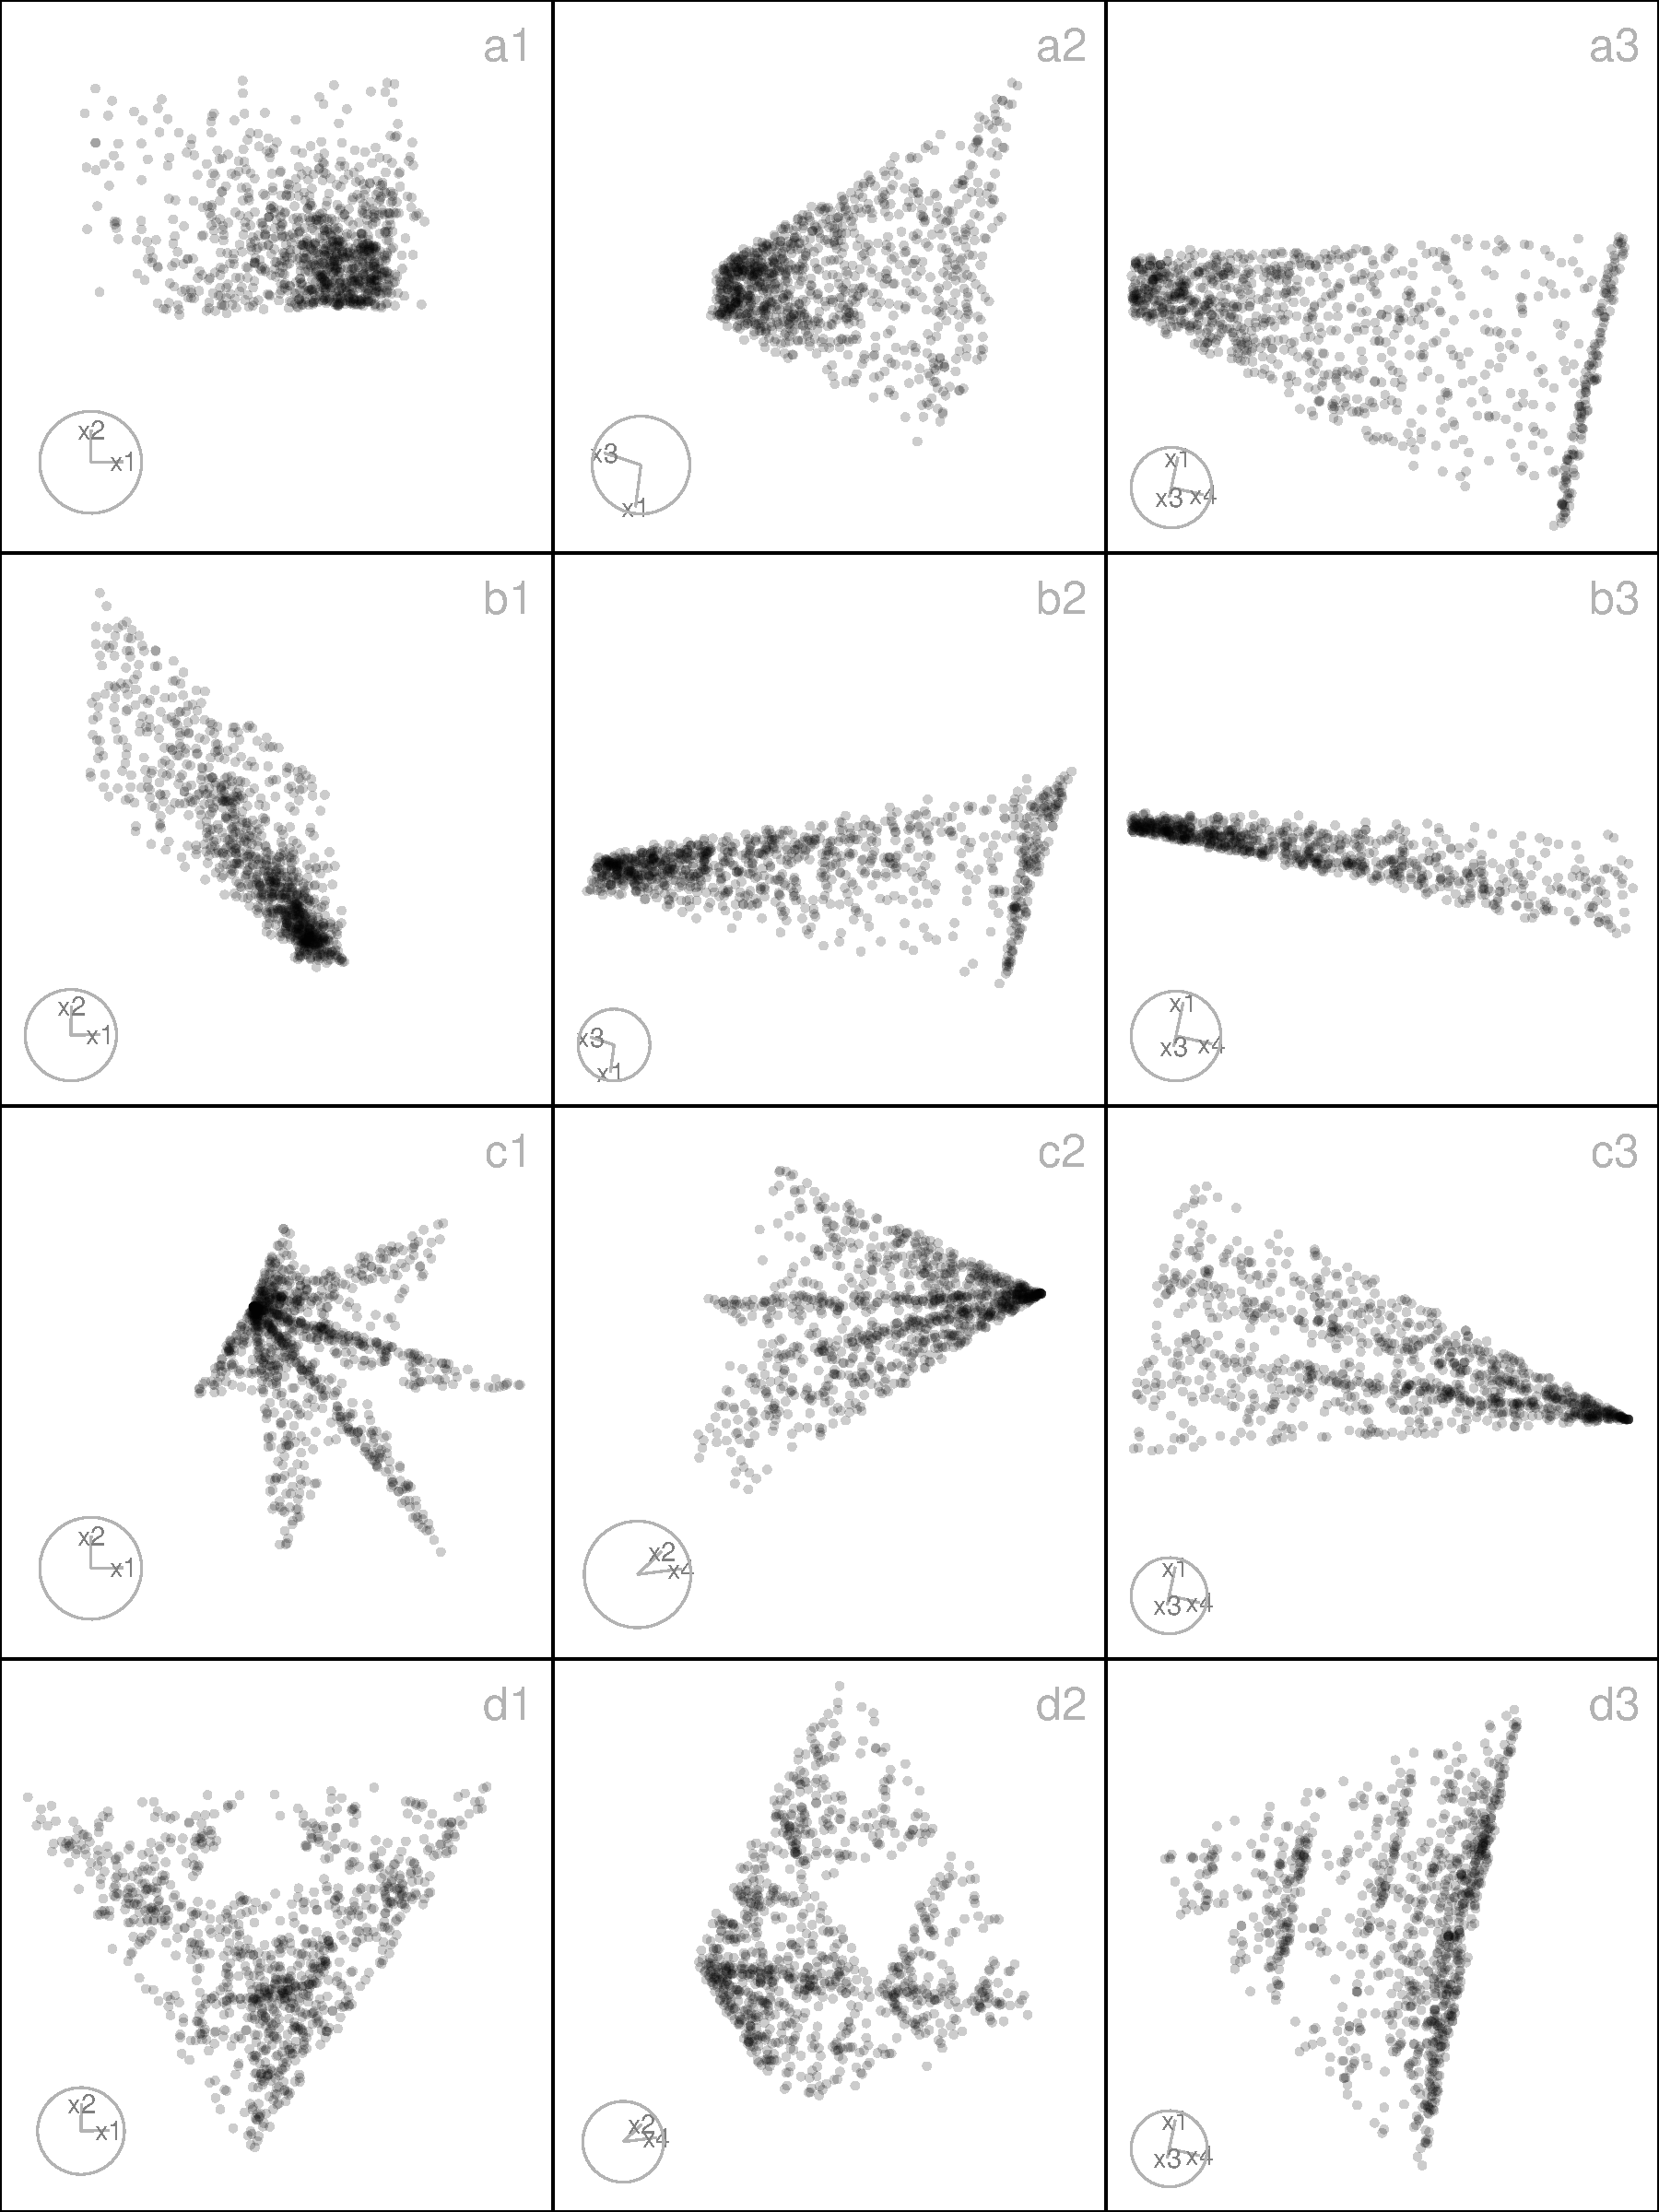
\includegraphics[width=1\linewidth,height=\textheight,keepaspectratio]{chapters/04-chap4_files/figure-pdf/pyr-proj-1.pdf}

}

\caption{Three \(2\text{-}D\) projections from \(4\text{-}D\), for the
\texttt{pyrrect} (a1-a3), \texttt{pyrtri} (b1-b3), \texttt{pyrstar}
(c1-c3), and \texttt{pyrholes} (d1-d3) data. The \texttt{pyrrrect}
structure forms a dense rectangular base tapering to a narrow tip, while
\texttt{pytri} shows a more triangular spread with sharper edges.
\texttt{Pyrstar} extends into multiple pointed branches radiating from a
common core, and \texttt{pyrholes} reveals hollow or open regions within
an otherwise compact shape. These projections illustrate a range of
pyramid-like geometries that vary in density and structure.}

\end{figure}%

\subsubsection{S-curve}\label{s-curve}

The S-curve is a smooth, non-linear manifold in \(3\text{-}D\) space.
Using \texttt{gen\_scurve(n)}, it is defined by
\(X_1 = \sin(\theta), \quad X_2 \sim U(0, 2), \quad X_3 = \text{sign}(\theta)(\cos(\theta) - 1), \quad \theta \sim U(-3\pi/2, 3\pi/2).\)

This follows the \texttt{s\_curve()} function from snedata
(\citeproc{ref-james2025}{\textbf{james2025?}}), itself adapted from
\emph{scikit-learn}, but differs by returning a tibble with standardized
names (\texttt{x1}, \texttt{x2}, \texttt{x3}), excluding the color
variable, and omitting built-in noise (which can be added separately).
S-curve is commonly used in manifold learning and dimension reduction as
benchmarks for unfolding curved structure.

\begin{Shaded}
\begin{Highlighting}[]
\NormalTok{scurve }\OtherTok{\textless{}{-}} \FunctionTok{gen\_scurve}\NormalTok{(}\AttributeTok{n =} \DecValTok{1000}\NormalTok{)}
\end{Highlighting}
\end{Shaded}

\subsubsection{Sphere}\label{sphere}

Sphere-shaped structures are useful for evaluating how dimension
reduction and clustering algorithms handle curved, symmetric manifolds
in high-dimensional spaces. The functions generate a variety of
spherical forms, including simple circles, uniform and hollow spheres,
grid-based spheres, and complex arrangements like clustered spheres
within a larger sphere. The first few coordinates define the main
geometric form (circle, cycle, sphere, or hemisphere), while
higher-dimensional embeddings are achieved by adding noise dimensions.
Such spherical or hemispherical structures frequently appear in physical
and biological systems, for example in models of celestial bodies,
molecular shells, or cell membranes
(\citeproc{ref-tinkham2003}{\textbf{tinkham2003?}};
\citeproc{ref-alberts2014}{\textbf{alberts2014?}}).Table
@ref(tab:sphere-tb-pdf) summarizes these functions.

\begin{table}

\caption{\label{tab:sphere-tb-pdf}cardinalR sphere data generation functions}
\centering
\begin{tabular}[t]{>{\raggedright\arraybackslash}p{4cm}>{\raggedright\arraybackslash}p{8cm}}
\toprule
Function & Explanation\\
\midrule
gen\_circle & Circle.\\
gen\_curvycycle & Curvy cell cycle.\\
gen\_unifsphere & Uniform sphere.\\
gen\_hollowsphere & Hollow sphere.\\
gen\_gridedsphere & Grided sphere.\\
gen\_clusteredspheres & Multiple small spheres within a big sphere.\\
gen\_hemisphere & Hemisphere.\\
\bottomrule
\end{tabular}
\end{table}

The simplest case, \texttt{gen\_circle(n,\ p)} creates a unit circle in
two dimensions, with the remaining dimensions forming sinusoidal
extensions of the angular parameter at progressively smaller scales
(Figure @ref(fig:sphere-proj) a). Let a latent angle variable \(\theta\)
is uniformly sampled from the interval \([0, 2\pi]\). Coordinates in the
first two dimensions represent a perfect circle on the plane:
\[X_1 = \cos(\theta), \quad X_2 = \sin(\theta).\] For dimensions \(X_3\)
through \(X_p\), sinusoidal transformations of the angle \(\theta\) are
introduced. The first component is a scaling factor that decreases with
the dimension index, defined as \(\text{scale}_j = \sqrt{(0.5)^{j-2}}\)
for \(j = 3, \dots, p\). The second component is a phase shift that is
proportional to the dimension index, specifically designed to
decorrelate the curves, given by the formula \(\phi_j = (j - 2)\pi/2p\).
Each additional dimension is computed as:
\(X_j = \text{scale}_{j}\sin(\theta + \phi_j), \quad j = 3, \dots, p\).

\begin{Shaded}
\begin{Highlighting}[]
\NormalTok{circle }\OtherTok{\textless{}{-}} \FunctionTok{gen\_circle}\NormalTok{(}\AttributeTok{n =} \DecValTok{1000}\NormalTok{, }\AttributeTok{p =} \DecValTok{4}\NormalTok{)}
\end{Highlighting}
\end{Shaded}

For the one-dimensional nonlinear cycle embedded in \(p\text{-}D\)
space, \texttt{gen\_curvycycle(n,\ p)} (Figure @ref(fig:sphere-proj) b),
let a latent angle variable \(\theta\) is uniformly sampled from the
interval \([0, 2\pi]\). The first three dimensions define a non-circular
closed curve, referred to as a ``curvy cycle''. In this configuration,
\(X_1 = \cos(\theta)\) represents horizontal oscillation, while
\(X_2 = \sqrt{3}/3 + \sin(\theta)\) introduces a vertical offset to
avoid centering the curve at the origin. Additionally,
\(X_3 = 1/3\cos(3\theta)\) introduces a third harmonic perturbation that
intricately folds the curve three times along its path, creating a
unique and complex shape that oscillates in both dimensions while
incorporating the effects of the harmonic perturbation.

Together, these define a periodic, non-trivial, closed curve in
\(3\text{-}D\) with internal folds that produce a more complex geometry
than a standard circle or ellipse. For dimensions \(X_4\) through
\(X_p\), additional structured variability is introduced through
decreasing amplitude scaling and phase-shifted sine waves. The scaling
factor is defined as \(\text{scale}_j = \sqrt{(0.5)^{j-3}}\) for \(j\)
ranging from \(4\) to \(p\), which means that the amplitude decreases as
the dimension increases. Each dimension \(X_j\) is then calculated using
the formula \(X_j = \text{scale}_j\sin(\theta + \phi_j)\), where the
phase shift \(\phi_j\) is given by \(\phi_j = (j - 2)\pi/2p\).

\begin{Shaded}
\begin{Highlighting}[]
\NormalTok{curvycycle }\OtherTok{\textless{}{-}} \FunctionTok{gen\_curvycycle}\NormalTok{(}\AttributeTok{n =} \DecValTok{1000}\NormalTok{, }\AttributeTok{p =} \DecValTok{4}\NormalTok{)}
\end{Highlighting}
\end{Shaded}

Building on simple circular structures, the
\texttt{gen\_unifsphere(n,\ r)} function function extends the idea to
three dimensions by generating \(n\) observations approximately
uniformly distributed on the surface of a sphere of radius \(r\).. Each
observation is computed from spherical coordinates, with
\(u \sim U(-1, 1)\) representing \(\cos(\phi)\) and
\(\theta \sim U(0, 2\pi)\) the azimuthal angle. Cartesian coordinates
are then defined as
\[X_1 = r\sqrt{1 - u^2}\cos(\theta), \quad X_2 = r\sqrt{1 - u^2}\sin(\theta),\text{ and }X_3 = ru,\]
ensuring uniform distribution on the surface (not within) of the sphere.

\begin{Shaded}
\begin{Highlighting}[]
\NormalTok{unifsphere }\OtherTok{\textless{}{-}} \FunctionTok{gen\_unifsphere}\NormalTok{(}\AttributeTok{n =} \DecValTok{1000}\NormalTok{, }\AttributeTok{r =} \DecValTok{1}\NormalTok{)}
\end{Highlighting}
\end{Shaded}

In contrast, the \texttt{gen\_hollowsphere(n,\ p)} function, a wrapper
around \texttt{geozoo::sphere.hollow()}, generates \(n\) points
uniformly distributed only on the surface of the \((p-1)\)-dimensional
sphere embedded in \(\mathbb{R}^p\). This results in a hollow shell-like
structure with no interior points. For example, when \(p=3\),
\texttt{gen\_unifsphere()} produces a solid ball in \(3\text{-}D\)
space, whereas \texttt{gen\_hollowsphere()} produces only the spherical
boundary. These paired structures allow controlled experiments to
investigate how algorithms behave when data is concentrated throughout
the full volume versus constrained to the boundary.

\begin{Shaded}
\begin{Highlighting}[]
\NormalTok{hollowsphere }\OtherTok{\textless{}{-}} \FunctionTok{gen\_hollowsphere}\NormalTok{(}\AttributeTok{n =} \DecValTok{1000}\NormalTok{, }\AttributeTok{p =} \DecValTok{4}\NormalTok{)}
\end{Highlighting}
\end{Shaded}

In addition, the \texttt{gen\_gridedsphere(n)} function constructs a
\(p\text{-}D\) dataset consisting of approximately \(n\) points that are
evenly distributed on the surface of the unit \((p-1)\)-sphere embedded
in \(\mathbb{R}^p\) (Figure @ref(fig:sphere-proj) d). The method relies
on forming a regular grid in spherical coordinates, parameterized by
\((p-1)\) angular variables: for dimensions \(j = 1, \dots, p-2\) the
polar angles are drawn from \([0, \pi]\), while the final angle
(\(j = p-1\)) represents the azimuth and is drawn from \([0, 2\pi]\).
The number of grid steps along each angular dimension is chosen by
decomposing \(n\) into \((p-1)\) approximately equal integer factors
using the helper function \texttt{gen\_nproduct(n,\ p\ -\ 1)}.

Each grid point is subsequently mapped into Cartesian space via the
standard hyperspherical-to-Cartesian transformation,

\[
\begin{aligned}
X_1 &= \cos(\theta_1), \\
X_2 &= \sin(\theta_1)\cos(\theta_2), \\
X_3 &= \sin(\theta_1)\sin(\theta_2)\cos(\theta_3), \\
&\;\;\vdots \\
X_{p-1} &= \sin(\theta_1)\sin(\theta_2)\cdots \sin(\theta_{p-2})\cos(\theta_{p-1}), \\
X_p &= \sin(\theta_1)\sin(\theta_2)\cdots \sin(\theta_{p-2})\sin(\theta_{p-1}).
\end{aligned}
\]

The result is a deterministic grid of points lying exactly on the
surface of the unit \((p-1)\)-sphere, without any additional noise
dimensions.

For more heterogeneous structures, the
\texttt{gen\_clusteredspheres(n,\ k,\ r,\ loc)} function generates one
large sphere of radius \(r_1\) and \(k\) smaller spheres of radius
\(r_2\), each centered at a different random location (Figure
@ref(fig:sphere-proj) e). A large uniform sphere centered at the origin
is created by sampling \(n_1\) points uniformly on the surface of a
\(p\text{-}D\) sphere with a radius of \(r_1\). The sampling is executed
using the function \texttt{gen\_unifsphere(n\_1,\ r\_1)}, which
generates the desired points in the specified dimensional space. In
generation of \(k\) smaller uniform spheres, each sphere contains
\(n_2\) points that are sampled uniformly on a sphere with a radius of
\(r_2\). These spheres are positioned at distinct random locations in
\(p\)-space, with the center of each sphere being drawn from a normal
distribution \(N(0, \texttt{loc}^2 I_p)\). Points on spheres are
generated using the standard hyperspherical method, which involves
sampling \(u \sim U(-1, 1)\) to determine the cosine of the polar angle,
and sampling \(\theta \sim U(0, 2\pi)\) to determine the azimuthal angle
(for \(3\text{-}D\)). Each observation is classified by cluster, with
labels such as ``big'' for the large central sphere and ``small\_1'' to
``small\_k'' for the smaller spheres.

\begin{Shaded}
\begin{Highlighting}[]
\NormalTok{clusteredspheres }\OtherTok{\textless{}{-}} \FunctionTok{gen\_clusteredspheres}\NormalTok{(}\AttributeTok{n =} \FunctionTok{c}\NormalTok{(}\DecValTok{1000}\NormalTok{, }\DecValTok{100}\NormalTok{), }\AttributeTok{k =} \DecValTok{3}\NormalTok{, }\AttributeTok{r =} \FunctionTok{c}\NormalTok{(}\DecValTok{15}\NormalTok{, }\DecValTok{3}\NormalTok{),}
                                         \AttributeTok{loc =} \DecValTok{10} \SpecialCharTok{/} \FunctionTok{sqrt}\NormalTok{(}\DecValTok{3}\NormalTok{)) }\SpecialCharTok{|\textgreater{}}
\NormalTok{  dplyr}\SpecialCharTok{::}\FunctionTok{select}\NormalTok{(}\SpecialCharTok{{-}}\NormalTok{cluster)}
\end{Highlighting}
\end{Shaded}

Finally, the \texttt{gen\_hemisphere(n,\ p)} function restricts sampling
to a hemisphere of a \(4\text{-}D\) sphere (Figure @ref(fig:sphere-proj)
f). Using spherical coordinates, the azimuthal angle
\(\theta_1 \sim U(0, \pi)\) in the \((x_1, x_2)\) plane, while the
elevation angle \(\theta_2 \sim U(0, \pi)\) in the \((x_2, x_3)\) plane.
Additionally, \(\theta_3 \sim U(0, \pi/2)\) in the \((x_3, x_4)\) plane,
ensuring that the points remain restricted to a hemisphere. The
coordinates are transformed into \(4\text{-}D\) Cartesian space:
\[X_1 = \sin(\theta_1)\cos(\theta_2), \quad X_2 = \sin(\theta_1)\sin(\theta_2), \quad X_3 = \cos(\theta_1)\cos(\theta_3), \quad X_4 = \cos(\theta_1)\sin(\theta_3).\]
This produces points on one side of a \(4\text{-}D\) unit sphere,
effectively generating a \(4\text{-}D\) hemisphere.

\begin{figure}[H]

{\centering 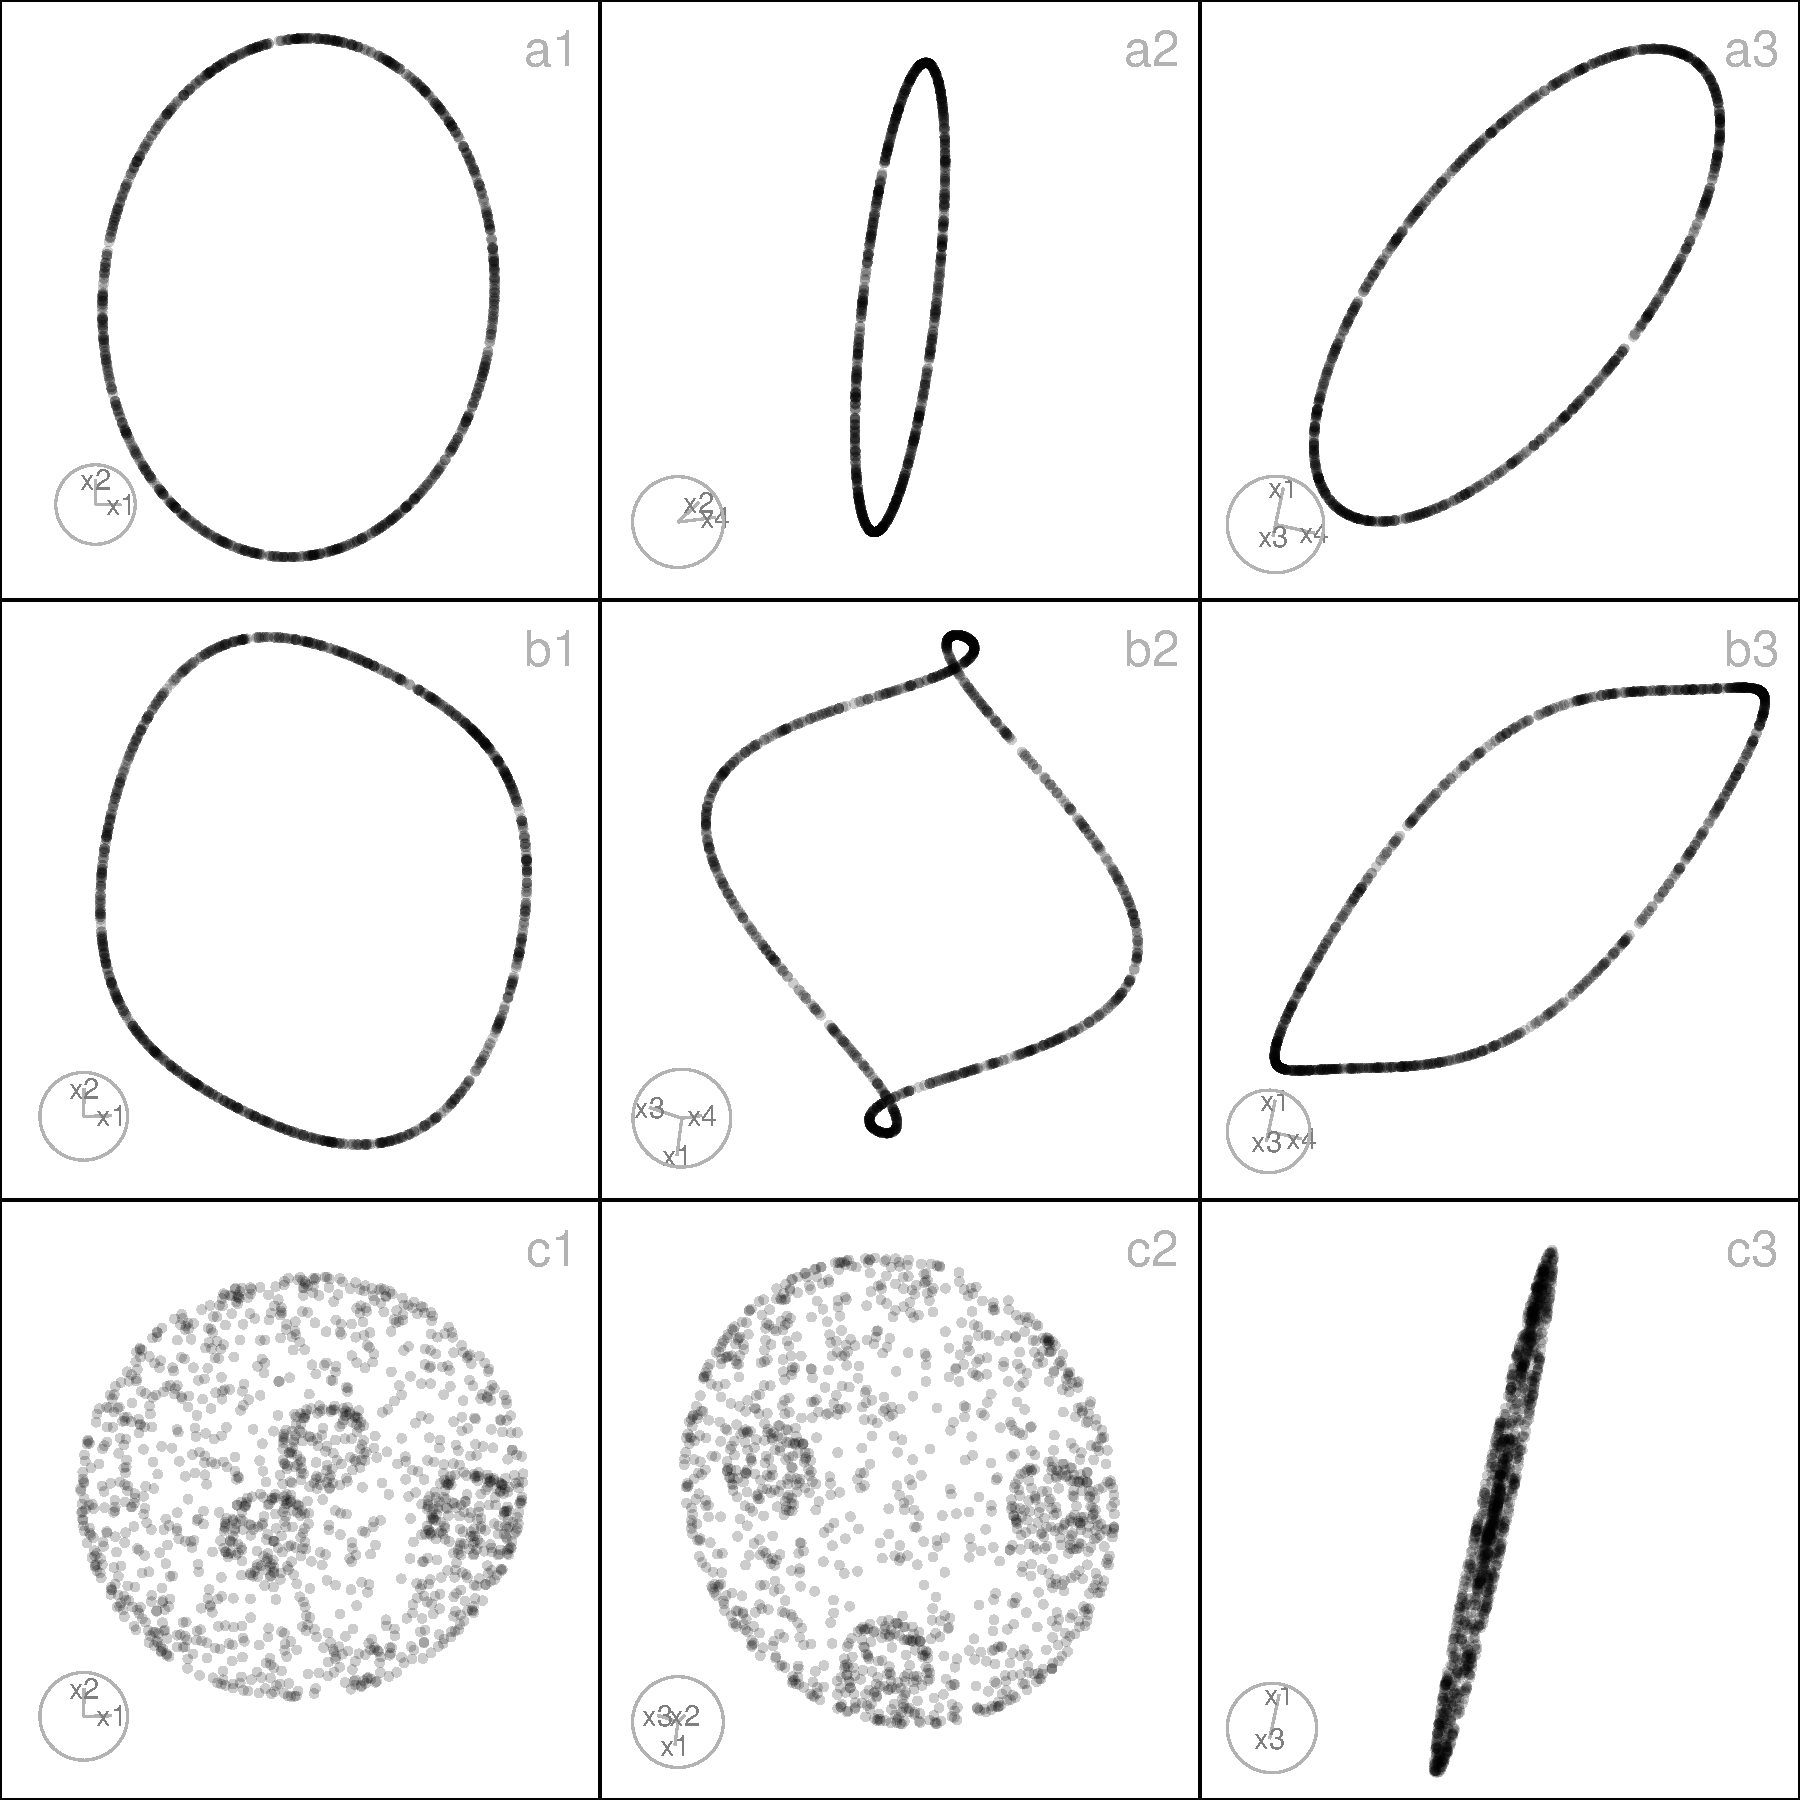
\includegraphics[width=1\linewidth,height=\textheight,keepaspectratio]{chapters/04-chap4_files/figure-pdf/sphere-proj-1.pdf}

}

\caption{Three \(2\text{-}D\) projections from \(4\text{-}D\),
\texttt{circle} (a1-a3), \texttt{curvycycle} (b1-b3), and,
\(3\text{-}D\) \texttt{clusteredspheres} (c1-c3). The \texttt{circle}
structure forms a smooth, closed loop, while \texttt{curvycycle} shows a
wavy, continuous pattern forming a twisted ring. The
\texttt{clusteredspheres} dataset displays multiple compact spherical
groups that are clearly separated in higher dimensions but overlap
slightly in some \(2\text{-}D\) projections, highlighting how projection
can distort spatial relationships. These projections show how simple
cyclic, wavy curvilinear, and clustered structures appear in
\(2\text{-}D\), emphasizing the effects of projection on density,
continuity, and separation}

\end{figure}%

\subsubsection{Swiss Roll}\label{swiss-roll}

The Swiss roll is a standard nonlinear manifold, representing a \gD{}
plane curled into \(3\text{-}D\). The \texttt{gen\_swissroll(n,\ w)}
generates points as
\(X_1 = t \cos(t), \quad X_2 = t \sin(t), \quad X_3 \sim U(w_1, w_2), \quad t \sim U(0, 3\pi).\)

\begin{Shaded}
\begin{Highlighting}[]
\NormalTok{swissroll }\OtherTok{\textless{}{-}} \FunctionTok{gen\_swissroll}\NormalTok{(}\AttributeTok{n =} \DecValTok{1000}\NormalTok{, }\AttributeTok{w =} \FunctionTok{c}\NormalTok{(}\SpecialCharTok{{-}}\DecValTok{1}\NormalTok{, }\DecValTok{1}\NormalTok{))}
\end{Highlighting}
\end{Shaded}

Compared with \texttt{sndata::swiss\_roll()}
(\citeproc{ref-james2025}{\textbf{james2025?}}), this implementation (i)
samples \(t\) over \([0, 3\pi]\) instead of \([1.5\pi, 4.5\pi]\), (ii)
allows a flexible vertical range \(w = (w_1, w_2)\) rather than fixing
\(z \in [0, z_{\max}]\), and (iii) returns a tibble with
\texttt{x1,\ x2,\ x3} instead of adding a color variable.

The Swiss roll is a classic benchmark for manifold learning,
illustrating how a curved surface can be ``unrolled'' into lower
dimensions. Similar spiral-like forms appear in galaxies, protein
folding, and coiled materials
(\citeproc{ref-dimitris2002}{\textbf{dimitris2002?}}).

\subsubsection{Trefoil knots}\label{trefoil-knots}

The Trefoil is a closed, nontrivial one-dimensional manifold embedded in
\(3\text{-}D\) or \(4\text{-}D\) space (Figure @ref(fig:trefoil-proj)).
The trefoil features topological complexity in the form of
self-overlaps, making it a valuable test case for evaluating the ability
of non-linear dimension reduction methods to preserve global structure,
loops, and embeddings in high-dimensional data. Table
@ref(tab:trefoil-tb-pdf) summarizes these functions.

\begin{table}

\caption{\label{tab:trefoil-tb-pdf}cardinalR trefoil data generation functions}
\centering
\begin{tabular}[t]{>{\raggedright\arraybackslash}p{4cm}>{\raggedright\arraybackslash}p{8cm}}
\toprule
Function & Explanation\\
\midrule
gen\_trefoil4d & Trefoil in 4-D.\\
gen\_trefoil3d & Trefoil in 3-D.\\
\bottomrule
\end{tabular}
\end{table}

For the \(4\text{-}D\) trefoil knot, the function
\texttt{gen\_trefoil4d(n,\ steps)} generates the structure on the
\(3\)-sphere (\(S^3 \subset \mathbb{R}^4\)) using two angular
parameters, \(\theta\) and \(\phi\). A band of thickness around the knot
path is controlled by the \texttt{steps} argument, while the number of
\(\theta\) and \(\phi\) values is determined by the \texttt{steps} and
\texttt{n} arguments, respectively (Figure @ref(fig:trefoil-proj) a).
The coordinates are defined as
\[X_1 = \cos(\theta) \cos(\phi), \quad X_2 = \cos(\theta) \sin(\phi), \quad X_3 = \sin(\theta) \cos(1.5 \phi),\text{ and }X_4 = \sin(\theta) \sin(1.5 \phi),\]
where \(\theta\) and \(\phi\) trace the knot's path.

\begin{Shaded}
\begin{Highlighting}[]
\NormalTok{trefoil4d }\OtherTok{\textless{}{-}} \FunctionTok{gen\_trefoil4d}\NormalTok{(}\AttributeTok{n =} \DecValTok{500}\NormalTok{, }\AttributeTok{steps =} \DecValTok{5}\NormalTok{)}
\end{Highlighting}
\end{Shaded}

For the \(3\text{-}D\) stereographic projection,
\texttt{gen\_trefoil3d(n,\ steps)} maps each point
\((X_1, X_2, X_3, X_4) \in \mathbb{R}^4\) to
\((X_1', X_2', X_3') \in \mathbb{R}^3\text{ using }X_1' = X_1 / (1 - X_4), \quad X_2' = X_2 / (1 - X_4),\text{ and }X_3' = X_3 / (1 - X_4),\)
excluding points where \(X_4 = 1\) to avoid division by zero (Figure
@ref(fig:trefoil-proj) b).

\begin{Shaded}
\begin{Highlighting}[]
\NormalTok{trefoil3d }\OtherTok{\textless{}{-}} \FunctionTok{gen\_trefoil3d}\NormalTok{(}\AttributeTok{n =} \DecValTok{500}\NormalTok{, }\AttributeTok{steps =} \DecValTok{5}\NormalTok{)}
\end{Highlighting}
\end{Shaded}

The trefoil knot appears in molecular biology (DNA/protein knotting),
fluid dynamics (knotted vortices), and physics (topological phases),
making it a useful benchmark for testing whether dimension reduction
preserves global loops and topology
(\citeproc{ref-witten1985}{\textbf{witten1985?}};
\citeproc{ref-arsuaga2002}{\textbf{arsuaga2002?}}).

\begin{figure}[H]

{\centering 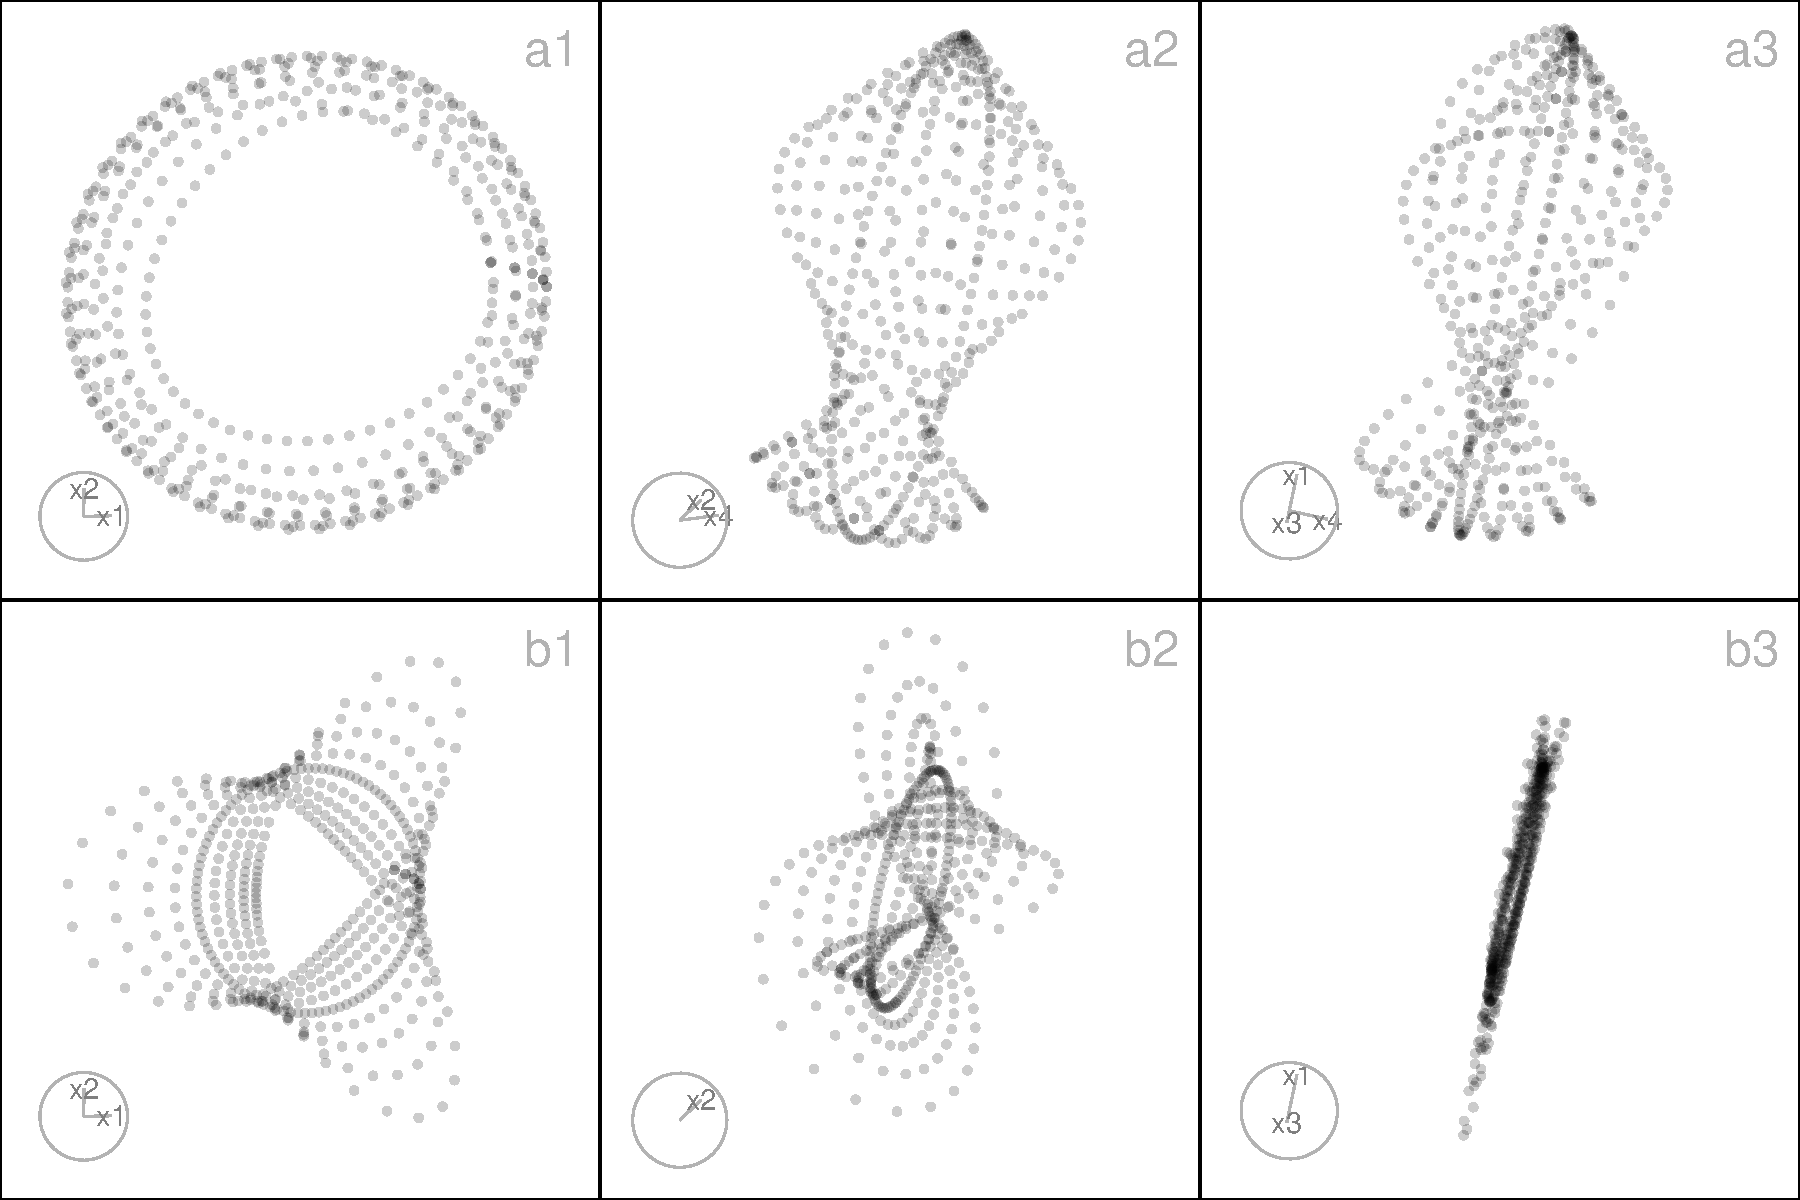
\includegraphics[width=1\linewidth,height=\textheight,keepaspectratio]{chapters/04-chap4_files/figure-pdf/trefoil-proj-1.pdf}

}

\caption{Three \(2\text{-}D\) projections from \(4\text{-}D\),
\texttt{trefoil4d} (a1-a3) and \(3\text{-}D\) \texttt{trefoil3d} (b1-b3)
data. The \texttt{trefoil4d} structure represents a higher-dimensional
extension of the classic trefoil knot, revealing complex twisting and
looping patterns that remain continuous across projections. In contrast,
the \texttt{trefoil3d} dataset maintains a simpler, more compact
knot-like form, showing how dimensional extension adds curvature and
separation in the embedded space. These projections illustrate a range
of looping structures in high-dimensions.}

\end{figure}%

\subsubsection{Trigonometric}\label{trigonometric}

Trigonometric-based structures provide flexible ways to simulate complex
curved patterns and spirals that often arise in real-world
high-dimensional data, such as in biological trajectories, or physical
systems (Figure @ref(fig:triginometric-proj)). The main geometry is
defined by the first few coordinates: crescents (\(p=2\)), cylinders,
spirals, and helices (\(p=4\)). These structures are particularly
valuable for testing how well dimension reduction and clustering
algorithms preserve intricate geometric and topological features
(\citeproc{ref-calladine1997}{\textbf{calladine1997?}};
\citeproc{ref-gershenfeld2000}{\textbf{gershenfeld2000?}}). Table
@ref(tab:trigonometric-tb-pdf) summarizes these functions.

\begin{table}

\caption{\label{tab:trigonometric-tb-pdf}cardinalR trigonometric data generation functions}
\centering
\begin{tabular}[t]{>{\raggedright\arraybackslash}p{4cm}>{\raggedright\arraybackslash}p{8cm}}
\toprule
Function & Explanation\\
\midrule
gen\_crescent & Crescent pattern.\\
gen\_curvycylinder & Curvy cylinder.\\
gen\_sphericalspiral & Spherical spiral.\\
gen\_helicalspiral & Helical spiral.\\
gen\_conicspiral & Conic spiral.\\
gen\_nonlinear & Nonlinear hyperbola.\\
\bottomrule
\end{tabular}
\end{table}

First, the \texttt{gen\_crescent(n,\ p)} function generates a
\(p\)-dimensional dataset of \(n\) observations based on a
\(2\text{-}D\) crescent-shaped manifold with optional structured
high-dimensional noise (Figure @ref(fig:triginometric-proj) a). Let
\(\theta \in [\pi/6, 2\pi]\) be a sequence of \(n\) evenly spaced
angles. The corresponding \(2\text{-}D\) coordinates are defined by:
\[X_1 = \cos(\theta), \quad X_2 = \sin(\theta).\]

\begin{Shaded}
\begin{Highlighting}[]
\NormalTok{crescent }\OtherTok{\textless{}{-}} \FunctionTok{gen\_crescent}\NormalTok{(}\AttributeTok{n =} \DecValTok{1000}\NormalTok{)}
\end{Highlighting}
\end{Shaded}

Second, the \texttt{gen\_curvycylinder(n,\ p,\ h)} function generates a
\(p\)-dimensional dataset of \(n\) observations structured as a
\(3\text{-}D\) cylindrical manifold with an added nonlinear curvy
dimension, and optional noise dimensions when \(p > 4\) (Figure
@ref(fig:triginometric-proj) b). The core structure consists of a
circular base and height values, extended by a nonlinear fourth
dimension. Let \(\theta \sim U(0, 3\pi)\) represent a random angle on a
circular base and \(z \sim U(0, h)\) represent the height along the
cylinder. The coordinates are defined as: \(X_1 = \cos(\theta)\)
(Circular base, x-axis), \(X_2 = \sin(\theta)\) (Circular base, y-axis),
\(X_3 = z\) (Linear height), and \(X_4 = \sin(z)\) (Nonlinear curvy
variation along height).

\begin{Shaded}
\begin{Highlighting}[]
\NormalTok{curvycylinder }\OtherTok{\textless{}{-}} \FunctionTok{gen\_curvycylinder}\NormalTok{(}\AttributeTok{n =} \DecValTok{1000}\NormalTok{, }\AttributeTok{h =} \DecValTok{10}\NormalTok{)}
\end{Highlighting}
\end{Shaded}

For a spiraling path on a spherical surface in the first four
dimensions, \texttt{gen\_sphericalspiral(n,\ p,\ spins)} (Figure
@ref(fig:triginometric-proj) c), let
\(\theta \in [0, 2\pi \times \text{spins}]\) be the azimuthal angle
(longitude), controls the number of spiral turns and the
\(\phi \in [0, \pi]\)be the polar angle (latitude), controls the
vertical sweep from the north to the south pole. Cartesian coordinates
from spherical conversion: \(X_1 = \sin(\phi)\cos(\theta)\),
\(X_2 = \sin(\phi)\sin(\theta)\), \(X_3 = \cos(\phi) + \varepsilon\),
where \(\varepsilon \sim U(-0.5, 0.5)\) introduces vertical jitter, and
\(X_4 = \theta / \max(\theta)\): a normalized progression along the
spiral path. This generates a spherical spiral curve embedded in
\(4\text{-}D\) space, combining both circular and vertical movement,
with gentle curvature and non-linear progression.

\begin{Shaded}
\begin{Highlighting}[]
\NormalTok{sphericalspiral }\OtherTok{\textless{}{-}} \FunctionTok{gen\_sphericalspiral}\NormalTok{(}\AttributeTok{n =} \DecValTok{1000}\NormalTok{, }\AttributeTok{spins =} \DecValTok{1}\NormalTok{)}
\end{Highlighting}
\end{Shaded}

For a helical spiral in four dimensions,
\texttt{gen\_helicalspiral(n,\ p)} (Figure @ref(fig:triginometric-proj)
d), let \(\theta \in [0, 5\pi/4]\) be a sequence of angles controlling
rotation around a circle. Cartesian coordinates; \(X_1 = \cos(\theta)\):
circular trajectory along the x-axis, \(X_2 = \sin(\theta)\): circular
trajectory along the y-axis, \(X_3 = 0.05\theta + \varepsilon_3\), with
\(\varepsilon_3 \sim U(-0.5, 0.5)\): linear progression (height) with
vertical jitter, simulating a helix, and \(X_4 = 0.1\sin(\theta)\):
oscillates with \(\theta\), representing a periodic ``wobble'' along the
fourth dimension.

\begin{Shaded}
\begin{Highlighting}[]
\NormalTok{helicalspiral }\OtherTok{\textless{}{-}} \FunctionTok{gen\_helicalspiral}\NormalTok{(}\AttributeTok{n =} \DecValTok{1000}\NormalTok{)}
\end{Highlighting}
\end{Shaded}

Similarly, the \texttt{gen\_conicspiral(n,\ p,\ spins)} function
generates a dataset of \(n\) points forming a conical spiral in the
first four dimensions of \(p\text{-}D\) (Figure
@ref(fig:triginometric-proj) e). The geometry combines radial expansion,
vertical elevation, and spiral deformation, simulating a structure that
fans out like a \(3\text{-}D\) conic helix. The shape is defined by
parameter \(\theta \in [0, 2\pi\text{spins}]\), controlling the angular
progression of the spiral. The Archimedean spiral in the horizontal
plane is represented by; \(X_1 = \theta\cos(\theta)\) for radial
expansion in x, and \(X_2 = \theta\sin(\theta)\) for radial expansion in
y. The growth pattern resembles a cone, with the height increasing
according to \(X_3 = 2\theta / \max(\theta) + \varepsilon_3\), with
\(\varepsilon_3 \sim U(-0.1, 0.6).\) Spiral modulation in the fourth
dimension is represented by
\(X_4 = \theta\sin(2\theta) + \varepsilon_4\), with
\(\varepsilon_4 \sim U(-0.1, 0.6)\) which simulates a twisting helical
component in a non-radial dimension.

\begin{Shaded}
\begin{Highlighting}[]
\NormalTok{conicspiral }\OtherTok{\textless{}{-}} \FunctionTok{gen\_conicspiral}\NormalTok{(}\AttributeTok{n =} \DecValTok{1000}\NormalTok{, }\AttributeTok{spins =} \DecValTok{1}\NormalTok{)}
\end{Highlighting}
\end{Shaded}

Finally, the \texttt{gen\_nonlinear(n,\ p,\ hc,\ non\_fac)} function
simulates a non-linear \(2\text{-}D\) surface embedded in higher
dimensions, constructed using inverse and trigonometric transformations
applied to independent variables (Figure @ref(fig:triginometric-proj)
f). The \(X_{1} \sim U(0.1, 2)\): base variable (avoids zero to prevent
division errors), \(X_{3} \sim U(0.1, 0.8)\): independent auxiliary
variable, \(X_{2} = hc/X_{1} + \text{nonfac}\sin(X_{1})\): non-linear
combination of hyperbolic and sinusoidal transformations, creating sharp
curvature and oscillation, and
\(X_{4} = \cos(\pi X_{1}) + \varepsilon\), with
\(\varepsilon \sim U(-0.1, 0.1)\): additional nonlinear variation based
on cosine, simulating more subtle periodic structure. These
transformations together result in a non-linear surface warped in
multiple ways: sharp vertical shifts due to inverse terms, smooth waves
from sine and cosine, and additional jitter.

\begin{Shaded}
\begin{Highlighting}[]
\NormalTok{nonlinear }\OtherTok{\textless{}{-}} \FunctionTok{gen\_nonlinear}\NormalTok{(}\AttributeTok{n =} \DecValTok{1000}\NormalTok{, }\AttributeTok{hc =} \DecValTok{1}\NormalTok{, }\AttributeTok{non\_fac =} \FloatTok{0.5}\NormalTok{)}
\end{Highlighting}
\end{Shaded}

\begin{figure}[H]

{\centering 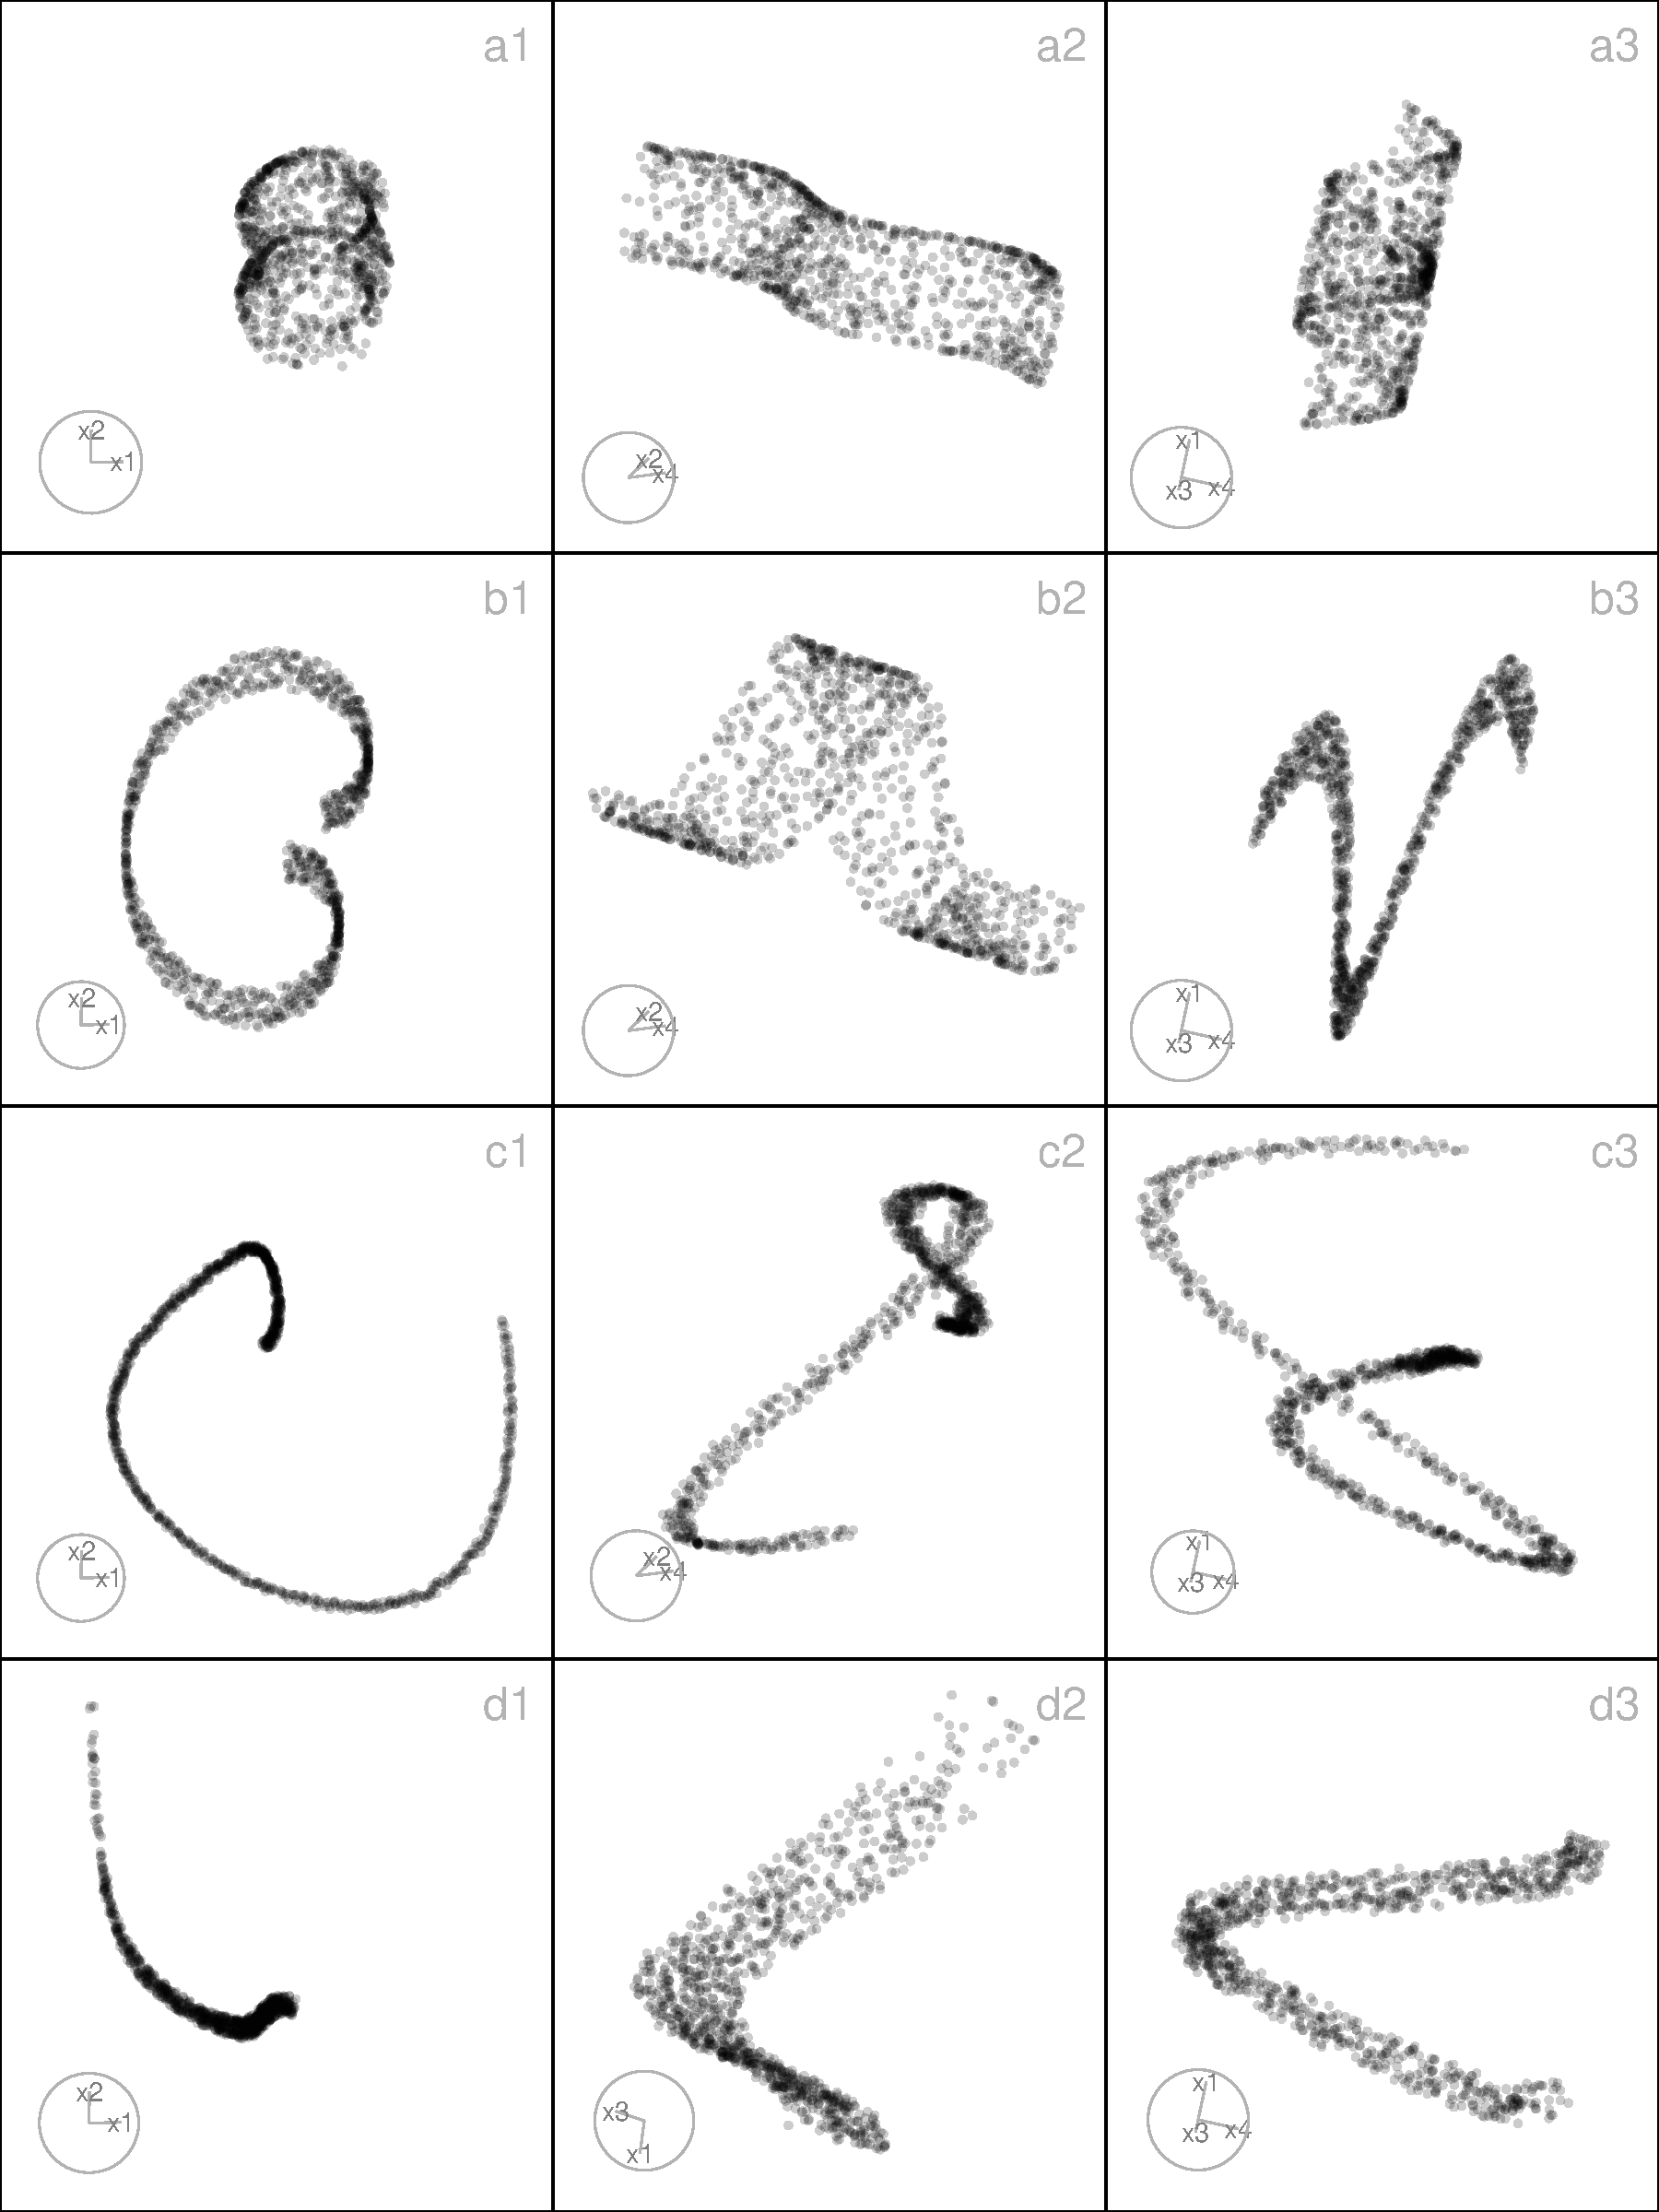
\includegraphics[width=1\linewidth,height=\textheight,keepaspectratio]{chapters/04-chap4_files/figure-pdf/triginometric-proj-1.pdf}

}

\caption{Three \(2\text{-}D\) projections from \(4\text{-}D\), for the
\texttt{curvycylinder} (a1-a3), \texttt{sphericalspiral} (b1-b3),
\texttt{conicspiral} (c1-c3), and \texttt{nonlinear} (d1-d3) data. The
\texttt{curvycylinder} shows a cylindrical manifold with a nonlinear
twist along its height, producing smooth, continuous curvature. The
\texttt{sphericalspiral} forms a spiral path on a spherical surface,
combining circular and vertical motion in a helical form. The
\texttt{conicspiral} spreads radially while ascending, forming a conical
helix with twisting variations in a non-radial dimension. The
\texttt{nonlinear} dataset exhibits a warped \(2\text{-}D\) surface with
sharp oscillations and smooth waves, reflecting complex nonlinear
interactions. Each shows variations in curvature, density, and
continuity.}

\end{figure}%

\subsection{Generate a spherical or hyperspherical hole within a
structure}\label{generate-a-spherical-or-hyperspherical-hole-within-a-structure}

The package provides functionality for generating datasets with
spherical hole (in \(2\text{-}D\)/\(3\text{-}D\)) or, more generally,
hyperspherical hole (in higher dimensions). These structures are
valuable for evaluating how dimension reduction methods and clustering
algorithms handle incomplete manifolds or missing regions of the data
space. A hyperspherical hole introduces topological complexity: the
structure remains continuous but contains excluded regions (voids) that
algorithms must correctly represent in lower-dimensional embeddings.

The core function \texttt{gen\_hole(df,\ anchor,\ r)} removes points
from a dataset that fall within a user-specified hypersphere. Formally,
given data points (\(x \in \mathbb{R}^p\)), a center
(\(a \in \mathbb{R}^p\)), and radius (\(r > 0\)), only points satisfying
\(||x - a||_2 > r\) are retained. The anchor point (\(a\)) can either be
user-specified or default to the dataset mean, and radius (\(r\)) is
controlled by the user, with safeguards to avoid trivial or degenerate
cases. Because it operates generically on any dataset, spherical or
hyperspherical holes can be embedded in a wide range of geometric
structures.

Two specialized wrappers illustrate this idea. The function
\texttt{gen\_scurvehole(n,\ r\_hole)} generates an S-curve with a
spherical hole by applying \texttt{gen\_hole()} to the output of
\texttt{gen\_scurve()}. This structure has been used in prior diagnostic
studies of NLDR methods, since it tests the ability of algorithms to
capture non-linear manifolds that are not simply connected. The second
wrapper, \texttt{gen\_unifcubehole(n,\ p,\ r\_hole)}, generates
uniformly sampled cube data with a hyperspherical hole. By embedding a
hyperspherical void inside a convex high-dimensional structure, this
creates non-convex regions that challenge algorithms in terms of
separability and neighborhood preservation.

\subsection{Generate noise dimensions}\label{generate-noise-dimensions}

High-dimensional data structures often benefit from the addition of
auxiliary noise dimensions, which can be used to assess the robustness
of dimensionality reduction and clustering algorithms. The functions in
this section provide flexible ways to generate random noise dimensions,
ranging from purely random Gaussian variables to more structured, wavy
patterns that mimic non-linear distortions in high-dimensional space.
These functions can be applied independently or combined with other
geometric structures to create complex simulated datasets. Table
@ref(tab:noise-tb-pdf) details these functions.

\begin{table}

\caption{\label{tab:noise-tb-pdf}cardinalR noise dimensions generation functions}
\centering
\begin{tabular}[t]{>{\raggedright\arraybackslash}p{2.5cm}>{\raggedright\arraybackslash}p{10.5cm}}
\toprule
Function & Explanation\\
\midrule
gen\_noisedims & Gaussian noise dimensions with optional mean and standard deviation.\\
gen\_wavydims1 & Wavy noise dimensions based on a user-specified theta sequence with added jitter.\\
gen\_wavydims2 & Wavy noise dimensions using polynomial transformations of an existing dimension vector.\\
gen\_wavydims3 & Wavy noise dimensions using a combination of polynomial and sine transformations based on the first three dimensions of a dataset.\\
\bottomrule
\end{tabular}
\end{table}

The \texttt{gen\_noisedims(n,\ p,\ m,\ s)} function generates \(p\)
independent Gaussian noise dimensions,

\[
X_j \sim N(m_j, s_j^2), \quad j = 1, \dots, p,
\]

with odd-numbered dimensions multiplied by \(-1\) to introduce sign
alternation, enhancing variability and decorrelation.

For scenarios where noise should follow a smooth wavy pattern,
\texttt{gen\_wavydims1(n,\ p,\ theta)} generates dimensions as

\[
X_j = \alpha_j \theta + \varepsilon_j, \quad \varepsilon_j \sim N(0, \sigma^2), \quad j = 1, \dots, p,
\]

where each dimension is scaled by a different factor \(\alpha_j\),
producing structured noise that oscillates along the latent parameter
\(\theta\), mimicking trends or trajectories observed in real-world
data.

The \texttt{gen\_wavydims2(n,\ p,\ x\_1)} function extends this approach
by applying a non-linear transformation to an existing dimension vector
\(x_1\):

\[
X_j = \beta_j \, (-1)^{\lfloor j/2 \rfloor} \, x_1^{k_j} + \varepsilon_j, \quad j = 1, \dots, p,
\]

where \(k_j\) is a randomly chosen polynomial power, \(\beta_j\) is a
scaling factor, and \(\varepsilon_j\) is small uniform noise.

Finally, \texttt{gen\_wavydims3(n,\ p,\ data)} generates noise for
datasets with multiple correlated dimensions. The first three dimensions
are small perturbations of the original coordinates \((X_1, X_2, X_3)\),
while higher dimensions are constructed via non-linear combinations,
including polynomial and trigonometric transformations, e.g.,

\[
X_j = f_j(X_1, X_2, X_3) + \varepsilon_j, \quad j > 3,
\]

producing high-dimensional noise that preserves some geometric
correlation with the base structure while introducing additional
complexity.

\subsection{Multiple cluster examples}\label{multiple-cluster-examples}

By using the shape generators mentioned above, we can create various
examples of multiple clusters. The package includes some of these
examples, which are described in Table @ref(tab:odd-shape-tb-pdf).

\begin{table}

\caption{\label{tab:odd-shape-tb-pdf}cardinalR multiple clusters generation functions}
\centering
\begin{tabular}[t]{>{\raggedright\arraybackslash}p{3.5cm}>{\raggedright\arraybackslash}p{8.5cm}}
\toprule
Function & Explanation\\
\midrule
make\_mobiusgau & Möbius-like cluster combined with a Gaussian.\\
make\_multigau & Multiple Gaussian clusters in high-dimensional space.\\
make\_curvygau & Curvilinear cluster with a Gaussian cluster.\\
make\_klink\_circles & K-link circular clusters (non-linear circular patterns).\\
make\_chain\_circles & Chain-like circular clusters connected sequentially.\\
make\_klink\_curvycycle & K-link curvy cycle clusters (curvilinear loop structures).\\
make\_chain\_curvycycle & Chain-like curvy cycle clusters connected sequentially.\\
make\_gaucircles & Circular clusters with a Gaussian cluster in the middle.\\
make\_gaucurvycycle & Curvy circular clusters with a Gaussian in the middle.\\
make\_onegrid & Single grid in two dimensions.\\
make\_twogrid\_overlap & Two overlapping grids.\\
make\_twogrid\_shift & Two grids shifted relative to each other.\\
make\_shape\_para & Parallel shaped clusters.\\
make\_three\_clust\_ & Three clusters with different shapes. (eg:- 01, 02, ..., 20)\\
\bottomrule
\end{tabular}
\end{table}

\subsection{Additional functions}\label{additional-functions}

The package includes various supplementary tools in addition to the
shape generating functions mentioned earlier. These tools allow users to
create background noise, randomize the rows of the data, relocate
clusters, generate a vector whose product and sum are approximately
equal to a target value, rotate structures, and normalize the data.
Table @ref(tab:add-tb-pdf) details these functions.

\begin{table}

\caption{\label{tab:add-tb-pdf}cardinalR additional functions}
\centering
\begin{tabular}[t]{>{\raggedright\arraybackslash}p{4cm}>{\raggedright\arraybackslash}p{8cm}}
\toprule
Function & Explanation\\
\midrule
gen\_bkgnoise & Adds background noise.\\
randomize\_rows & Randomizes the rows.\\
relocate\_clusters & Relocates the clusters.\\
gen\_nproduct & Generates a vector of positive integers whose product is approximately equal to a target value.\\
gen\_nsum & Generates a vector of positive integers whose summation is approximately equal to a target value.\\
gen\_rotation & Generates rotations.\\
normalize\_data & Normalizes data.\\
\bottomrule
\end{tabular}
\end{table}

\section{Application}\label{application-1}

This section demonstrates how the package can be used to generate
complex high-dimensional datasets, apply dimension reduction (DR)
techniques, and evaluate clustering performance. The example shows how
diverse geometric structures can be simulated and analyzed to assess
algorithmic behavior.

\subsection{Generating high-dimensional clustered
data}\label{generating-high-dimensional-clustered-data}

To illustrate, we generate a dataset with five clusters in
\(4\text{-}D\), each representing distinct geometric characteristics: a
\emph{helical spiral} (elongated and twisted), a \emph{hemisphere}
(curved surface), a \emph{uniform cube} (isotropic distribution), a
\emph{cone} (density gradient), and a \emph{Gaussian} cluster (compact
and spherical) (Figure @ref(fig:highd-proj)). Each cluster has a unique
number of points and scaling factor, representing variation in cluster
size and spread across the \(4\text{-}D\) space.

\begin{Shaded}
\begin{Highlighting}[]
\NormalTok{positions }\OtherTok{\textless{}{-}}\NormalTok{ geozoo}\SpecialCharTok{::}\FunctionTok{simplex}\NormalTok{(}\AttributeTok{p=}\DecValTok{4}\NormalTok{)}\SpecialCharTok{$}\NormalTok{points}
\NormalTok{positions }\OtherTok{\textless{}{-}}\NormalTok{ positions }\SpecialCharTok{*} \FloatTok{0.3}

\DocumentationTok{\#\# To generate data}
\NormalTok{five\_clusts }\OtherTok{\textless{}{-}} \FunctionTok{gen\_multicluster}\NormalTok{(}\AttributeTok{n =} \FunctionTok{c}\NormalTok{(}\DecValTok{2250}\NormalTok{, }\DecValTok{1500}\NormalTok{, }\DecValTok{750}\NormalTok{, }\DecValTok{1250}\NormalTok{, }\DecValTok{1750}\NormalTok{), }\AttributeTok{k =} \DecValTok{5}\NormalTok{,}
                       \AttributeTok{loc =}\NormalTok{ positions,}
                       \AttributeTok{scale =} \FunctionTok{c}\NormalTok{(}\FloatTok{0.25}\NormalTok{, }\FloatTok{0.35}\NormalTok{, }\FloatTok{0.3}\NormalTok{, }\DecValTok{1}\NormalTok{, }\FloatTok{0.3}\NormalTok{),}
                       \AttributeTok{shape =} \FunctionTok{c}\NormalTok{(}\StringTok{"helicalspiral"}\NormalTok{, }\StringTok{"hemisphere"}\NormalTok{, }\StringTok{"unifcube"}\NormalTok{, }
                                 \StringTok{"cone"}\NormalTok{, }\StringTok{"gaussian"}\NormalTok{),}
                       \AttributeTok{rotation =} \ConstantTok{NULL}\NormalTok{,}
                       \AttributeTok{is\_bkg =} \ConstantTok{FALSE}\NormalTok{)}
\end{Highlighting}
\end{Shaded}

\begin{figure}[H]

{\centering 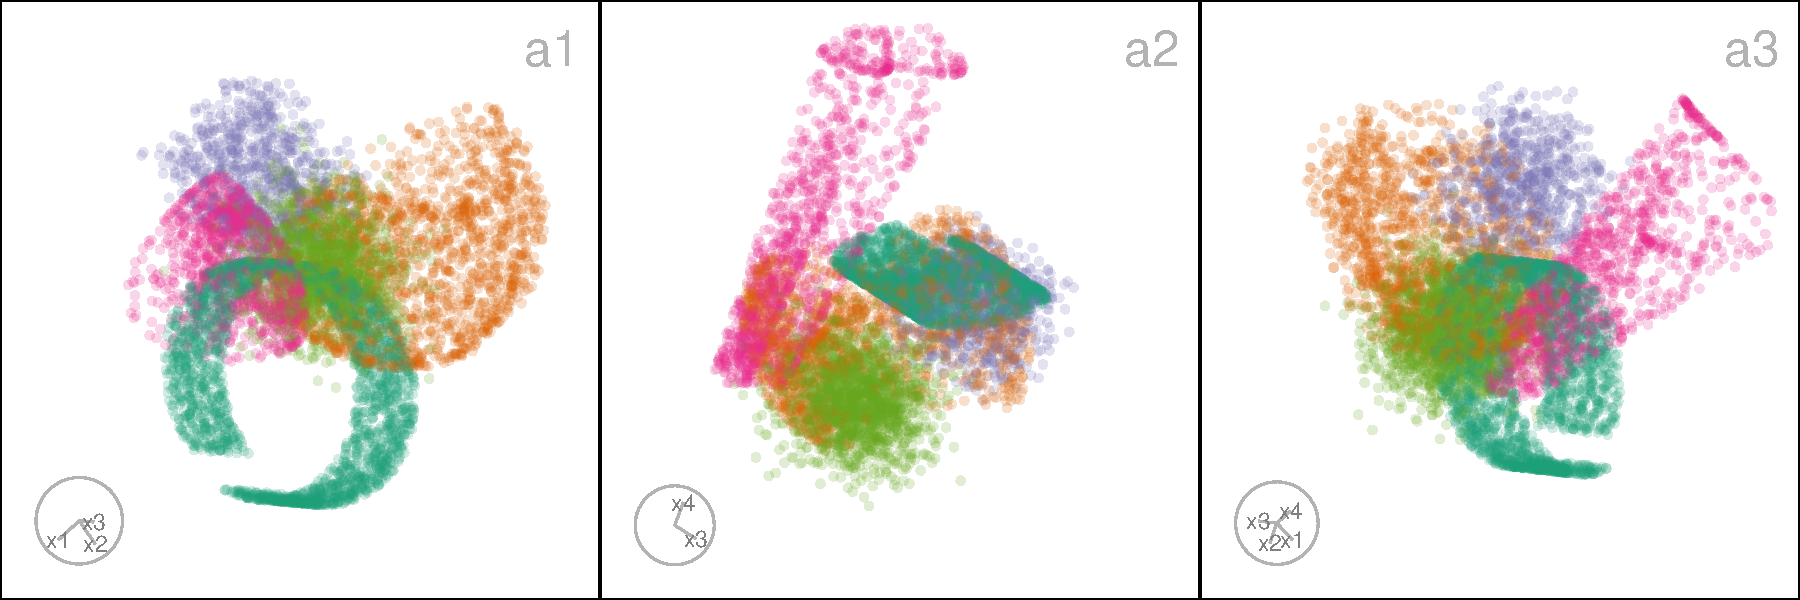
\includegraphics[width=1\linewidth,height=\textheight,keepaspectratio]{chapters/04-chap4_files/figure-pdf/highd-proj-1.pdf}

}

\caption{Three \(2\text{-}D\) projections from \(4\text{-}D\), for the
five clusters data. The helical spiral cluster is represented in dark
green, the hemisphere cluster in orange, the uniform cube-shaped cluster
in purple, the blunted cone cluster in pink, and the Gaussian-shaped
cluster in light green.}

\end{figure}%

\subsection{Evaluating dimension reduction (DR)
methods}\label{evaluating-dimension-reduction-dr-methods}

We applied six popular DR techniques to the generated dataset: Principal
Component Analysis (PCA) (\citeproc{ref-jolliffe2011}{Jolliffe 2011}),
t-distributed stochastic neighbor embedding (tSNE)
(\citeproc{ref-laurens2008}{Maaten and Hinton 2008}), uniform manifold
approximation and projection (UMAP) (\citeproc{ref-leland2018}{McInnes
et al. 2018}), potential of heat-diffusion for affinity-based trajectory
embedding (PHATE) algorithm (\citeproc{ref-moon2019}{Moon et al. 2019}),
large-scale dimensionality reduction Using triplets (TriMAP)
(\citeproc{ref-amid2019}{\textbf{amid2019?}}), and pairwise controlled
manifold approximation (PaCMAP) (\citeproc{ref-yingfan2021}{Wang et al.
2021}).

\begin{figure}[H]

\centering{

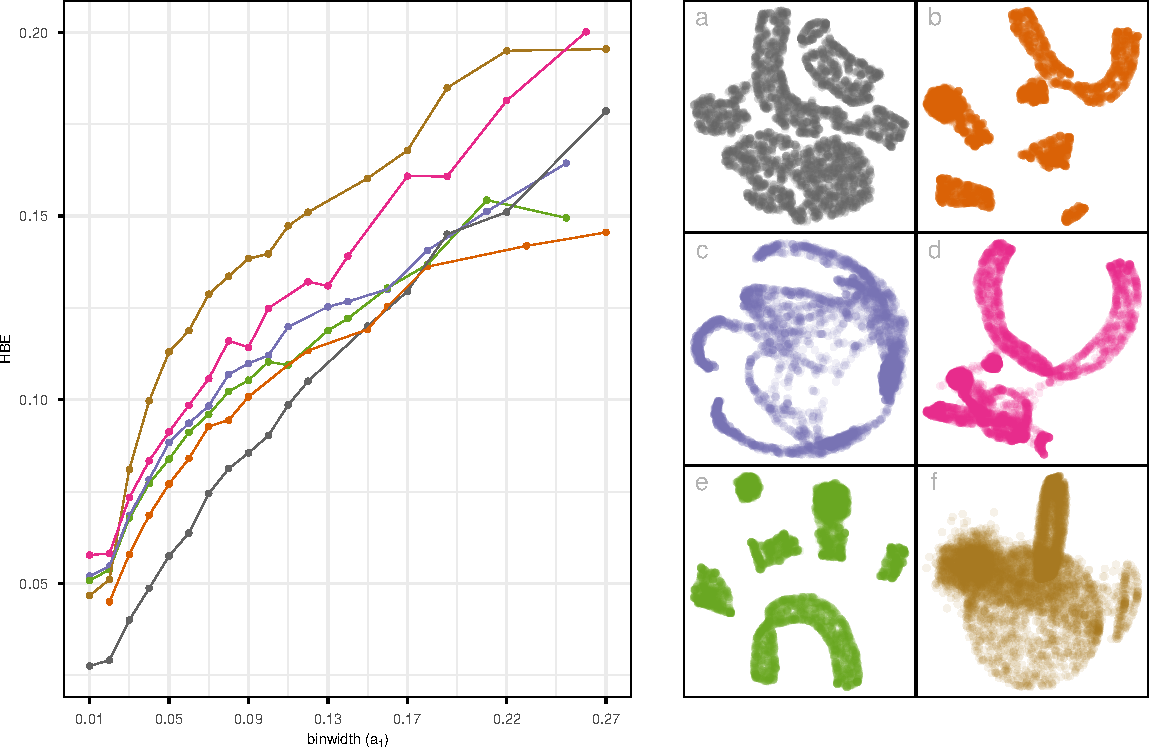
\includegraphics[width=1\linewidth,height=\textheight,keepaspectratio]{chapters/04-chap4_files/figure-pdf/fig-nldr-layouts-1.pdf}

}

\caption{\label{fig-nldr-layouts}Assessing which of the 6 NLDR layouts
((a) tSNE, (b) UMAP, (c) PAHTE, (d) TriMAP, (e) PaCMAP, and (f) PCA) of
the five clusters data is the better representation using RMSE for
varying binwidth (\(a_1\)). Colour is used for the lines and points in
the left plot to match the scatterplots of the NLDR layouts (a-f).
Layout f is universally poor. Layouts a and b are universally optimal.
Layout b shows six well-separated clusters and latout a shows close
clusters, thus layout a is the best choice.}

\end{figure}%

To assess their performance, we computed the root mean squared error
(RMSE) between the observed high-dimensional data and the fitted values,
defined as the high-dimensional mappings of the bin centroids
(\citeproc{ref-gamage2025c}{\textbf{gamage2025c?}}). A lower RMSE
indicates that the method better preserves the high-dimensional
structure in its low-dimensional embedding.

As shown in Figure @ref(fig:fig-nldr-layouts), tSNE (Figure
@ref(fig:fig-nldr-layouts) a) achieved the lowest RMSE across bin widths
(mostly tiny), indicating high preservation of both local and global
structures. Its layout displays well-separated clusters with minimal
inter-cluster distances, making it the most faithful representation of
the underlying data structure. UMAP and PaCMAP (Figure
@ref(fig:fig-nldr-layouts) b and e) produced moderately accurate
embeddings, although the six clusters appear more well-separated, while
PHATE (Figure @ref(fig:fig-nldr-layouts) c) show non-linear cluster
structures irrespective of the original structure. Also, TriMAP (Figure
@ref(fig:fig-nldr-layouts) d) has high RMSE, and show three clusters
with small distances. PCA (Figure @ref(fig:fig-nldr-layouts) f) failed
to capture the non-linear geometry, leading to the highest RMSE.

\subsection{Benchmarking clustering
algorithms}\label{benchmarking-clustering-algorithms}

To further evaluate the structure of the generated data, we benchmarked
three clustering algorithms: \textbf{\(k\)-means} (Chapter 20 of
\citeproc{ref-boehmke2019}{\textbf{boehmke2019?}}),
\textbf{hierarchical}
(\citeproc{ref-murtagh2012}{\textbf{murtagh2012?}}), and
\textbf{model-based clustering}
(\citeproc{ref-chris2002}{\textbf{chris2002?}};
\citeproc{ref-scrucca2023}{\textbf{scrucca2023?}}) using the simulated
dataset. The model-based clustering was performed with the
\texttt{"VVV"} covariance structure, allowing each cluster to vary in
volume, shape, and orientation. Cluster validity statistics were
computed using the \texttt{cluster.stats()} function from the
\texttt{fpc} package
(\citeproc{ref-christian2024}{\textbf{christian2024?}}).

\begin{table}

\caption{\label{tab:summaryclust-tb-pdf}Comparison of clustering performance metrics (within–between ratio (wb.ratio), Dunn index, Corrected Rand index, and variation of information (VI) across $k$-means, hierarchical, and model-based clustering methods.}
\centering
\begin{tabular}[t]{>{\raggedright\arraybackslash}p{2.5cm}>{\raggedleft\arraybackslash}p{2cm}>{\raggedleft\arraybackslash}p{2cm}>{\raggedleft\arraybackslash}p{2.5cm}>{\raggedleft\arraybackslash}p{2cm}}
\toprule
Metric & wb.ratio & Dunn Index & Corrected Rand & VI\\
\midrule
k-means & 0.61 & 0.01 & 0.42 & 1.32\\
Hierarchical & 0.61 & 0.01 & 0.50 & 1.15\\
Model-based & 0.61 & 0.01 & 0.75 & 0.65\\
\bottomrule
\end{tabular}
\end{table}

Overall, all methods produced similar compactness and separation, as
reflected by the \emph{within--between cluster ratios (wb.ratio)} and
\emph{Dunn indices}. However, the \textbf{model-based clustering}
achieved the highest \emph{Corrected Rand Index} (\(0.75\)) and lowest
\emph{Variation of Information (VI)} (\(0.65\)), indicating the best
recovery of the true underlying groups (Table
@ref(tab:summaryclust-tb-pdf)). In comparison, \(k\)-means and
hierarchical clustering showed moderate agreement with the true labels.
These findings demonstrate that mixture-based approaches can more
effectively capture the heterogeneity of clusters in high-dimensional,
non-spherical data.

\section{Conclusion}\label{conclusion}

The \texttt{cardinalR} package introduces a flexible framework for
generating high-dimensional data structures with well-defined geometric
properties. It addresses an important need in the evaluation of
clustering, machine learning, and DR methods by enabling the
construction of customized datasets with interpretable structures, noise
characteristics, and clustering arrangements. In this way,
\texttt{cardinalR} complements existing packages such as
\texttt{geozoo}, \texttt{snedata}, and \texttt{mlbench}, while extending
the scope to higher dimensions and more complex shapes.

The motivation for developing this package originated from the need to
design a perception--misperception experiment, aimed at investigating
how well NLDR methods preserve inter-cluster structure. To conduct this
study, we required simulated datasets with carefully controlled
geometric and clustering properties. While some existing packages
provided useful starting points, none fully supported the creation of
flexible, high-dimensional data with the specific structural variations
needed for our experiment. Developing these generators for research
purposes gradually led to the design of \texttt{cardinalR} as a
general-purpose package, so that other researchers can benefit from the
same tools for simulation, benchmarking, and teaching.

The included structures cover a wide range of diagnostic settings.
Branching shapes facilitate the study of continuity and topological
preservation, the Scurve with a hole allows investigation of incomplete
manifolds, and clustered spheres assess separability on curved surfaces.
The Möbius strip introduces challenges from non-orientable geometry,
while gridded cubes and pyrholes test spatial regularity and clustering
in sparse, non-convex regions.

These structures are designed to support not only algorithm diagnostics,
but also teaching high-dimensional concepts, benchmarking
reproducibility, and evaluating hyperparameter sensitivity. By allowing
users to adjust dimensionality, sample size, noise, and clustering
properties, the package promotes transparent experimentation and
comparative model evaluation.

Future extensions of \texttt{cardinalR} may include biologically
inspired or application-driven data structures would further broaden its
utility in domains such as bioinformatics, forensic science, and spatial
analysis.

\section{Acknowledgements}\label{acknowledgements-2}

The source material for this paper is available at
\href{https://github.com/JayaniLakshika/paper-cardinalR}{github.com/JayaniLakshika/paper-cardinalR}.
This article is created using \texttt{knitr}
(\citeproc{ref-yihui2015}{\textbf{yihui2015?}}) and \texttt{rmarkdown}
(\citeproc{ref-yihui2018}{\textbf{yihui2018?}}) in R with the
\texttt{rjtools::rjournal\_article} template. These \texttt{R} packages
were used for this work: \texttt{cli}
(\citeproc{ref-gabor2025}{\textbf{gabor2025?}}), \texttt{tibble}
(\citeproc{ref-kirill2023}{\textbf{kirill2023?}}), \texttt{gtools}
(\citeproc{ref-gregory2023}{\textbf{gregory2023?}}), \texttt{dplyr}
(\citeproc{ref-hadley2023}{Wickham 2023}), \texttt{stats}
(\citeproc{ref-core2025}{\textbf{core2025?}}), \texttt{tidyr}
(\citeproc{ref-hadley2024}{\textbf{hadley2024?}}), \texttt{purrr}
(\citeproc{ref-hadley2025}{\textbf{hadley2025?}}), \texttt{mvtnorm}
(\citeproc{ref-alan2009}{\textbf{alan2009?}}), \texttt{geozoo}
(\citeproc{ref-barret2016}{\textbf{barret2016?}}), and \texttt{MASS}
(\citeproc{ref-venables2002}{\textbf{venables2002?}}).

\bookmarksetup{startatroot}

\chapter{Perception and Misperception in Nonlinear Dimension Reduction:
A User Study}\label{sec-second-paper}

\section{Introduction}\label{introduction-3}

Non-linear dimension reduction (NLDR) is popular for making a suitable
\gD{} representation of high-dimensional (\pD{}) data by applying
non-linear transformations. Recently developed methods include
t-distributed stochastic neighbor embedding (tSNE)
(\citeproc{ref-laurens2008}{Maaten and Hinton 2008}), uniform manifold
approximation and projection (UMAP) (\citeproc{ref-leland2018}{McInnes
et al. 2018}), potential of heat-diffusion for affinity-based trajectory
embedding (PHATE) algorithm (\citeproc{ref-moon2019}{Moon et al. 2019}),
large-scale dimensionality reduction Using triplets (TriMAP)
(\citeproc{ref-amid2022}{Amid and Warmuth 2022}), and pairwise
controlled manifold approximation (PaCMAP)
(\citeproc{ref-yingfan2021}{Wang et al. 2021}). However, in different
data structures, the \gD{} representation generated can vary
dramatically from what is observed in \pD{}
(Figure~\ref{fig-nldr-layouts}).

\begin{figure}[H]

\centering{

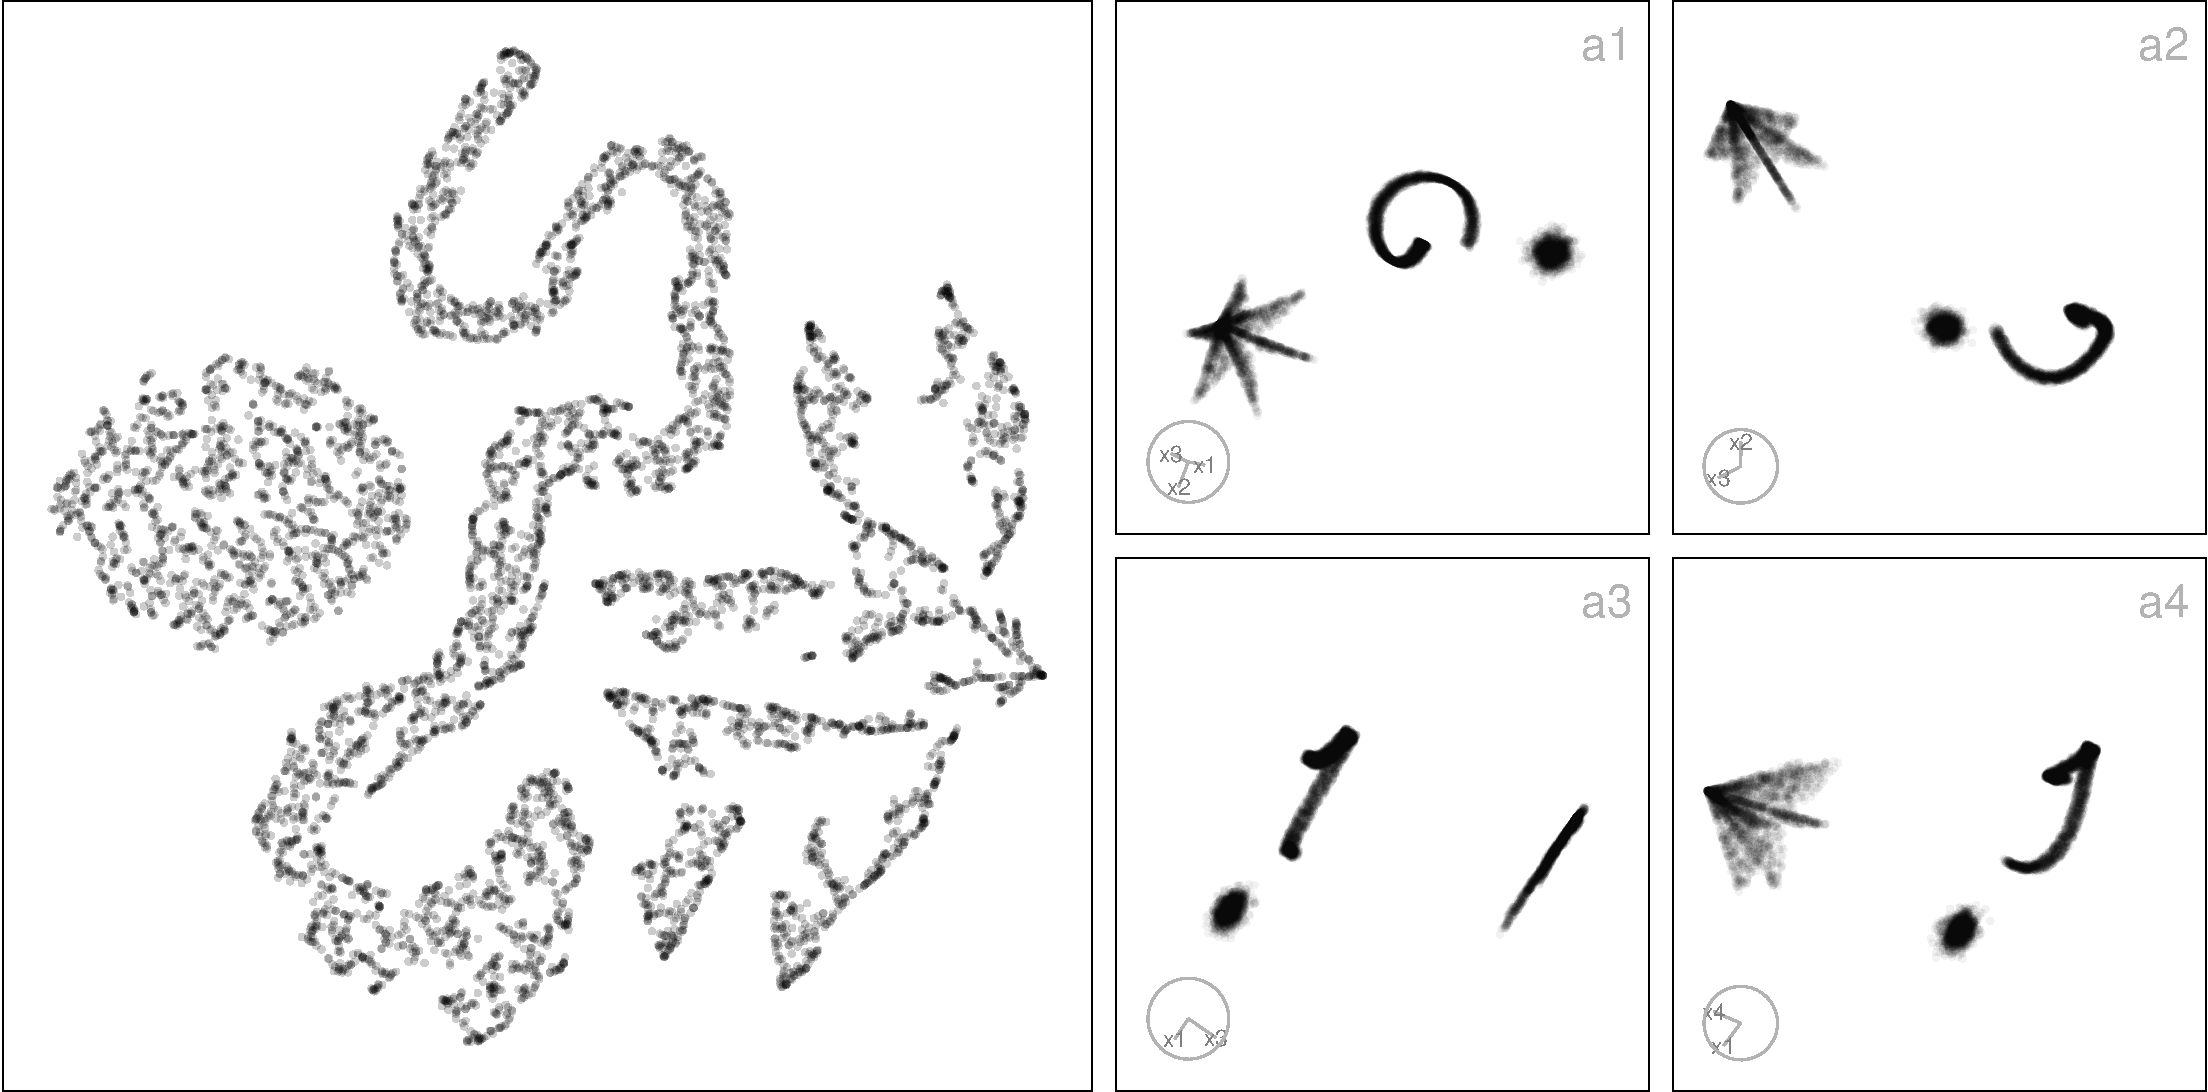
\includegraphics[width=1\linewidth,height=\textheight,keepaspectratio]{chapters/05-chap5_files/figure-pdf/fig-nldr-layouts-1.pdf}

}

\caption{\label{fig-nldr-layouts}A \gD{} tSNE layout (left) and four
\gD{} projections (a1--a4) of the same \hD{} data. The data consist of
three main structures: a star-shaped, a curvilinear, and a
Gaussian-shaped clusters. While the tour consistently show the
star-shaped cluster as a single coherent group, the \gD{} tSNE layout
fragments this structure into several smaller clusters. This illustrates
how NLDR may distort global structure, making the same \hD{} cluster
appear as multiple clusters in the \gD{} layout.}

\end{figure}%

The dilemma for the analyst is then understanding \textbf{why viewers
misidentify the data displayed in the \gD{} NLDR layout and
high-dimensional view when the inter-cluster distance vary}. The
research described here provides evidence through a cognitive perception
experiment.

The paper is organized as follows. Section~\ref{sec-background} provides
a summary of the literature on NLDR, high-dimensional data, and
visualization methods. Section~\ref{sec-experiment} describes the
experiment designed to examine people's perception to assess how viewers
recognize structure differently from the NLDR layout and the tour view.
Section~\ref{sec-results} discusses the collected data and results.
Limitations are provided in Section~\ref{sec-limitations}. A discussion
of the presented work, and ideas for future directions are described in
Chapter~\ref{sec-conclusion}.

\section{Background}\label{sec-background}

Historically, \gD{} representations of \pD{} data have been obtained
through techniques based on multidimensional scaling (MDS)
(\citeproc{ref-kruskal1964}{Kruskal 1964}), including principal
component analysis (PCA) (for an overview see Jolliffe
(\citeproc{ref-jolliffe2011}{2011})). These methods aim to construct a
\gD{} layout that preserves pairwise distances between observations in
the original space by minimizing a stress function. Variants such as
non-metric scaling (\citeproc{ref-saeed2018}{Saeed et al. 2018}) and
isomap (\citeproc{ref-silva2002}{Silva and Tenenbaum 2002}) extend this
approach to capture nonlinear relationships. Challenges inherent to
high-dimensional data visualization---such as distance concentration and
interpretability---are well recognized
(\citeproc{ref-johnstone2009}{Johnstone and Titterington 2009}).

Several NLDR methods have since become popular for generating \gD{}
representations that aim to preserve either local or global structures
of \gD{} data. Examples include tSNE, UMAP, PHATE, TriMAP, and PaCMAP.
Each method uses different underlying principles---for example, tSNE and
PHATE emphasize local relationships, while TriMAP and PaCMAP are
designed to better capture global structure. As a result, these methods
can produce very different \gD{} layouts of the same data, potentially
leading to misinterpretation of structures such as cluster separation.

An alternative to NLDR for visualizing \pD{} data is to use linear
projections. PCA is the classical approach, producing new variables as
linear combinations of the original dimensions. While PCA provides a
single static projection that maximizes variance, tours---introduced by
Asimov (\citeproc{ref-As85}{1985})---extend this idea by generating
smooth sequences of linear projections, effectively creating a movie of
the data viewed from multiple directions. Tours can reveal structure
that may be hidden in any single projection by continuously changing the
viewing angle through high-dimensional space. Many tour algorithms have
since been developed and are implemented in the R package tourr
(\citeproc{ref-wickham2011}{Wickham et al. 2011}), with interactive
variants available in langevitour (\citeproc{ref-harisson2024}{Harrison
2023}) and detourr (\citeproc{ref-hart2022}{Hart and Wang 2022}). Tours
are valuable because they preserve the true linear geometry of the
data---unlike NLDR methods, they do not warp distances or angles. This
makes them faithful but sometimes visually cluttered representations:
global structure can obscure local detail, and the phenomenon of piling
(\citeproc{ref-laa2022}{Laa et al. 2022})---where high-dimensional
points project toward the center---can make clusters harder to
distinguish.

To assess how well NLDR methods preserve structures such as cluster
separation, it is important to quantify inter-cluster distances. A
variety of distance-based metrics have been proposed in the clustering
and visualization literature
(\citeproc{ref-tadeusz1974}{\textbf{tadeusz1974?}};
\citeproc{ref-peter1987}{\textbf{peter1987?}};
\citeproc{ref-david1979}{\textbf{david1979?}}), including minimum,
maximum, and average distances between clusters, centroid distances, and
ratios that combine between- and within-cluster variation. In this
study, we focus on two complementary measures: the between-to-within
(BW) ratio, which captures global separability, and the minimum distance
between clusters, which reflects the closest approach of any two
clusters. Together, these provide interpretable summaries of both
overall and local cluster separation while accounting for within-cluster
variability.

The objective of this research is to conduct a cognitive perception
experiment that examines how participants recognize and interpret
structure differently when viewing a two-dimensional NLDR layout and a
tour, generated with langevitour. We investigate how perceived structure
changes as true cluster separation (as measured by BW ratio and minimum
distance) increases, and how this perception differs across methods.
These findings will help identify common misperceptions that can arise
when analysts rely solely on NLDR layouts, and will inform better
practice in interpreting and reporting structures seen in such
visualizations.

\section{Method}\label{sec-experiment}

\subsection{\texorpdfstring{What is a \gD{} NLDR
plot?}{What is a  NLDR plot?}}\label{what-is-a-nldr-plot}

The \gD{} representation of the high-dimensional data constructed to
preserve as much information, like clustering and non-linear
relationships, as possible. There are various commonly used techniques
for creating this \gD{} representation, including tSNE, and UMAP. These
methods aim to identify a low-dimensional structure that captures the
most important patterns or relationships in the data, allowing for
visualization and easier interpretation. However, it is important to
note that \gD{} embeddings can lose some information from the
high-dimensional data, as they necessarily involve a loss of
dimensionality.

\subsection{What is a tour?}\label{what-is-a-tour}

The tour shows a sequence of two-dimensional linear projections of the
high-dimensional data. It is similar to looking at shadows of a
\(3\text{-}D\) object, and trying to infer the shape of the
\(3\text{-}D\) object. Looking at linear projections of high-dimensional
data is like looking at the shadows, and one hopes to gain a sense of
what shapes exist in the data. For example, if the data separates into
clusters in any of the projections, it means that there are clusters in
the data in the high dimensions. If the data shows a non-linear or
curvilinear shape it means that there are non-linear associations
between some variables. If the data collapses to roughly a line it means
that it lives in a lower dimensional space than the number of high
dimensions. If the points moving differently from others, there are
outliers or unusual observations in the high dimensions.

\subsection{What is being tested?}\label{what-is-being-tested}

We are generally interested in testing whether ``The two plots displays
the same data'' (\(H_0\)) against the broad alternative ``The two plots
do not display the same data'' (\(H_a\)).

Testing this broad null hypothesis (\(H_0\)) is practically challenging
due to the variety of data structures involved. It can be both
time-consuming and computationally intensive. Therefore, we focused on
one data structure that is particularly useful for investigation: three
clusters where two clusters are close together, while one is more
distant. Three clusters have different shapes and each cluster contain
different number of points. The sample size is \(7500\).

Our hypothesis is as follows:

\(H_{0m1}\): The distance between the clusters has no effect on the
probability of correctly identifying the \gD{} NLDR plot generated by
NLDR method \(m\) and the tour from the same data. Vs \(H_{1m1}\): The
distance between the clusters does have an effect on the probability of
correctly identifying the \gD{} NLDR plot generated by NLDR method \(m\)
and the tour from the same data.

This study aims to answer which NLDR methods are more accurate in
identifying the same data structure in the \gD{} NLDR plot and the tour,
as the distance increases, and to identify which types of data structure
components are more prone to misidentification across methods.

\subsection{Data generation}\label{data-generation}

For non-attention check attempts, \(28\) data structures are generated,
while only two data structures are generated for attention check
attempts. Before being presented to participants, the data is
\emph{scaled}.

\subsubsection{Non-attention check data}\label{non-attention-check-data}

For the experiment, three cluster data are generated. The three clusters
contain different number of points and shapes. Let \(C_1, C_2,\) and
\(C_3\) denote the centroids of three clusters. The pairwise distances
between these centroids are calculated as:
\(d(C_1, C_2) = c_{12} \approx 2.17, \quad d(C_1, C_3) = c_{13} \approx 4, \quad d(C_2, C_3) \approx c_{23} = 3.6\).
These results indicate that clusters \(C_1\) and \(C_2\) are in close
proximity, whereas cluster \(C_3\) is positioned further away from the
other two clusters, suggesting a spatial separation within the data. The
reason for using the distance between centroids is that it can be easily
controlled.

In total, there are \(28\) data structures used for the experiment. Out
of these, \(18\) data structures show the same structure in both the
\gD{} NLDR plot and tour for each experiment, while the remaining \(10\)
data structures display different structures in the \gD{} NLDR plot and
tour. This means that when data structure \(19\) is displayed in the
NLDR plot, data structure \(20\) appears in the tour.

To systematically vary the degree of separation in the SAME trials, the
original (medium large) centroid distances are scaled by four different
factors: \(0.1\) (small), \(0.6\) (small medium), \(0.9\) (medium), and
\(1.1\) (large). In contrast, data structures used for the DIFFERENT
trials retained the original (medium-large) centroid distances.

\subsubsection{Attention check data}\label{attention-check-data}

There are two sets of attention check data; one consisting of three
Gaussian clusters and the other consisting of four Gaussian clusters.
Each cluster is generated using a multivariate normal distribution where
the mean vectors and variances were predefined. Specifically, for the
three-cluster case, the mean vectors were set as \([1, 0, 0, 0]\),
\([0, 1, 0, 0]\), and \([0, 0, 1, 1]\), with a common variance of
\(0.1\) for all clusters. For the four-cluster case, the mean vectors
were defined as \([1, 0, 0, 1]\), \([0, 1, 1, 0]\), \([1, 0, 1, 0]\),
and \([0, 1, 0, 1]\), also using a variance of \(0.1\). This approach
ensures that data points are normally distributed around the specified
centroids, with the spread controlled by the variance parameter. Each
Gaussian cluster dataset consists of \hD{} data with a sample size of
\(7500\), and each cluster contains an equal number of data points.

\subsection{Experiment design}\label{experiment-design}

The visual layout of the experiment for one participant is shown in
Figure~\ref{fig-exp-design}. Each participant completed \(20\) trials:
\(15\) SAME trials, in which the same data structure was shown in both
the \gD{} NLDR plot and the tour; \(4\) DIFFERENT trials, showing
DIFFERENT data structures; and one attention check trial that could be
either SAME or DIFFERENT. For the SAME, five NLDR methods (\emph{tSNE,
UMAP, PHATE, PaCMAP, and TriMAP}) were each paired with three of five
distance scale factors (\emph{small, small medium, medium, medium large,
and large}), giving \(15\) balanced combinations. In the DIFFERENT, four
NLDR methods were randomly selected, with the remaining method assigned
to the attention check trial. All DIFFERENT and attention check trials
used a distance scale factor of \emph{medium large}.

\begin{figure}

\centering{

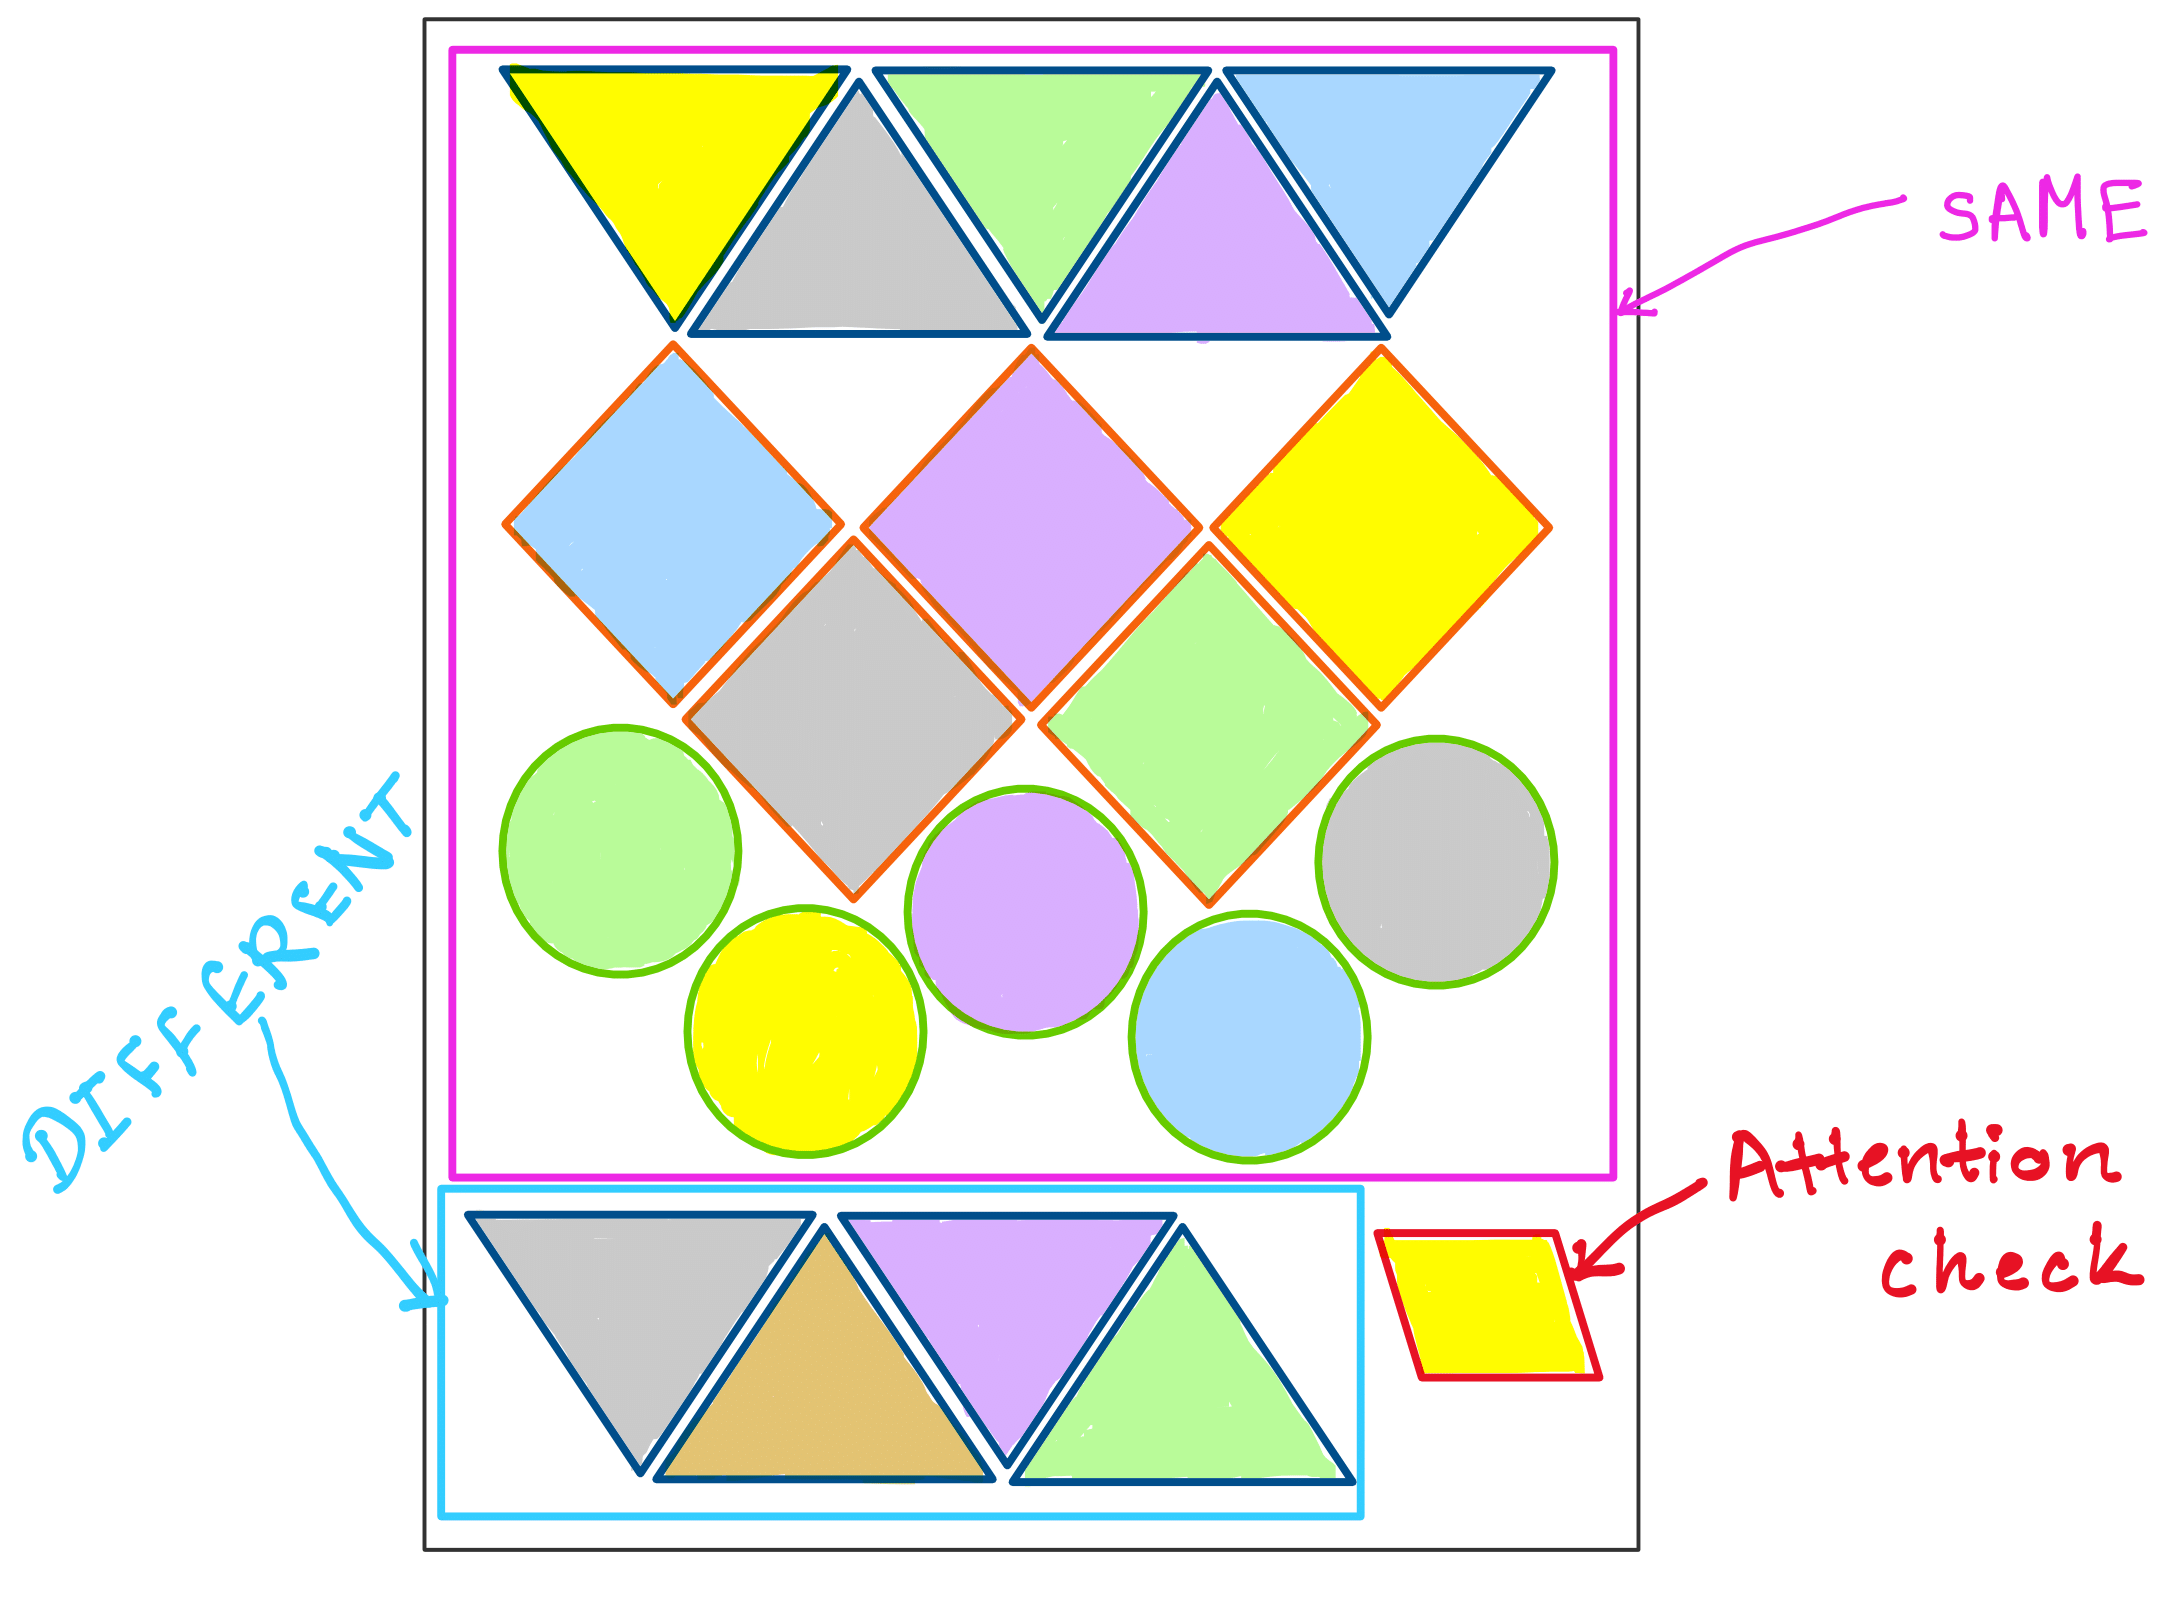
\includegraphics[width=1\linewidth,height=\textheight,keepaspectratio]{chapters/../figures/vis-exp/exp_design.png}

}

\caption{\label{fig-exp-design}Experiment design for one participant.
Shapes represent distance scale factors, and fill colors denote NLDR
methods. Each participant completed 20 trials: \(15\) SAME trials
showing the same data structure in both the \gD{} plot and tour
(purple), \(4\) DIFFERENT trials showing different structures (light
blue), and one attention check (SAME or DIFFERENT) (red). In SAME
trials, five NLDR methods (tSNE, UMAP, PHATE, TriMAP, and PaCMAP) were
combined with three of five distance scale factors (small, small medium,
medium, medium large, and large). For DIFFERENT trials, four NLDR
methods were randomly selected, and the remaining method was used in the
attention check. All DIFFERENT and attention check trials used a
distance scale factor of \emph{medium large}.}

\end{figure}%

\subsection{Treatments}\label{treatments}

Two primary treatments were considered in the experiment: the NLDR
method and the distance scale factor.

The first treatment consisted of five NLDR methods: \emph{tSNE, UMAP,
PHATE, PaCMAP, and TriMAP} each producing a \gD{} representation.

The second treatment, the distance scale factor, controlled the degree
of cluster separation in the high-dimensional space. Five categorical
levels: \emph{small, small--medium, medium, medium--large, and large}
were defined to represent increasing degrees of separability. This
categorical design enhances interpretability and perceptual
distinctness, allowing participants to discern meaningful structural
differences while maintaining robustness against minor data variations.

Cluster separability was quantified using two complementary measures:
the \emph{between-to-within (BW) ratio} and the \emph{minimum
inter-cluster distance}. A higher value of either metric indicates
greater separation among clusters (Figure~\ref{fig-dist-metrics}).

The BW ratio, defined as

\[
\text{BW Ratio} = \frac{B}{W} = \frac{ \sum_{i=1}^{3} n_i \cdot \|\bar{\mathbf{x}}_i - \bar{\mathbf{x}}\|^2 }{ \sum_{i=1}^{3} \sum_{\mathbf{x}_j \in C_i} \|\mathbf{x}_j - \bar{\mathbf{x}}_i\|^2 }.
\]

where (B) and (W) denote between- and within-cluster dispersion,
respectively; \(\bar{\mathbf{x}}_i\) is the centroid of cluster \(C_i\);
\(\bar{\mathbf{x}}\) is the overall centroid; and \(n_i\) is the number
of observations in cluster \(C_i\).

In addition, the minimum distance was used as a complementary measure of
global separation:

\[
\text{minimum distance} = \min_{k \neq \ell} \min_{x \in C_k, , y \in C_\ell} d(x, y),
\]

which captures the closest proximity between any two clusters.

\begin{figure}

\centering{

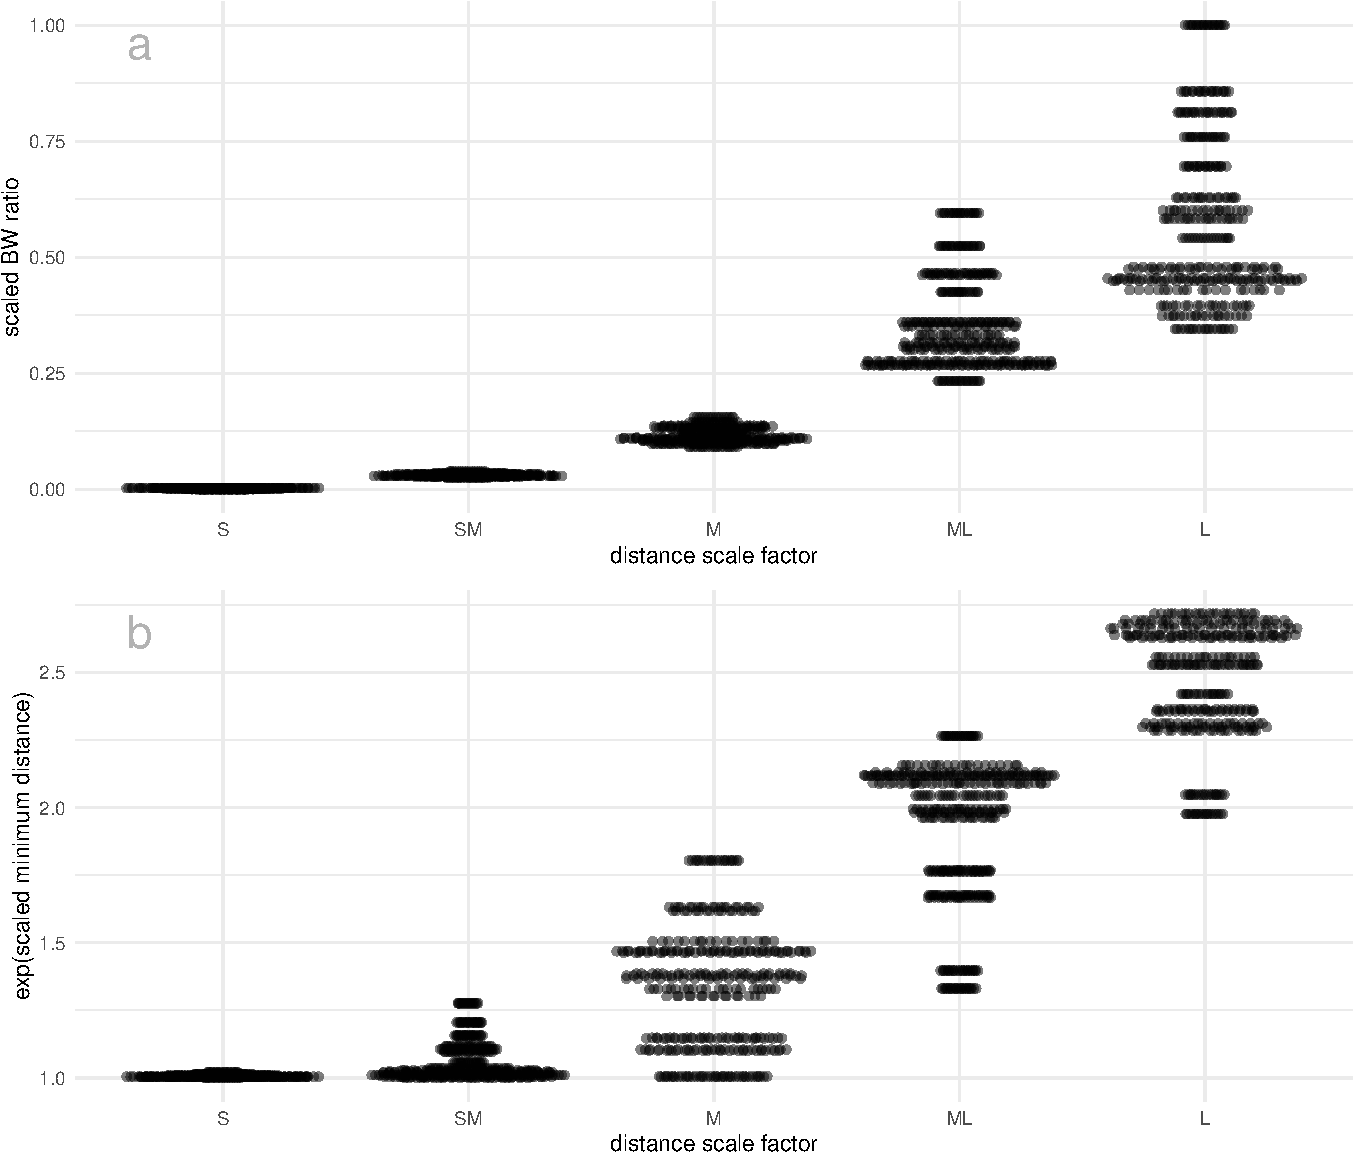
\includegraphics[width=1\linewidth,height=\textheight,keepaspectratio]{chapters/05-chap5_files/figure-pdf/fig-dist-metrics-1.pdf}

}

\caption{\label{fig-dist-metrics}Distribution of distance metric values
across distance scale factors used as treatments in the experiment. (a)
Between-to-within (BW) ratio and (b) minimum inter-cluster distance,
each plotted against five categorical distance scale factors: small (S),
small--medium (SM), medium (M), medium--large (ML), and large (L). Both
metrics increase systematically with the scale factor, confirming that
the distance scale treatment effectively controls cluster separability
in the high-dimensional space.}

\end{figure}%

\subsection{Participant recruitment}\label{participant-recruitment}

Participants were recruited from the Prolific crowd-sourcing platform
(\citeproc{ref-palan2018}{\textbf{palan2018?}}). The study expects that
the participants are uninvolved judges with no prior knowledge of the
data to avoid inadvertently affecting results. Pre-screening procedures
were applied the recruitment: potential participants needed with fluent
in English and have completed at least 10 Prolific studies with a 98\%
approval rate.

\subsection{Data collection}\label{data-collection}

The survey web application,
\href{https://ebsmonash.shinyapps.io/web_game/}{Match-a-roo} was used
for data collection. Participants provided introduction and instructions
for the survey. Before start the survey, the participants can lead to
the ``example'' page which allow them to experiment with the data
collection interface and practice deciding whether the two displays
shown the same data or not. The main purpose of using the ``example''
was merely intended to familiarize the participants with the questions
which would be asked as well as the process of deciding whether the two
displays shown the same data or not. The interface did not provide any
numeric feedback as to participant correctness.

The participants were asked to provide their Prolific ID and their
consent to the responses being used for analysis. After giving consent,
the participant can start the trials. Two visual displays of data were
shown where the data may be the SAME or DIFFERENT. One of the visual
displays is a \gD{} NLDR plot, and the other is a tour. The participants
were asked to decide whether that data was the same in both displays and
to report their confidence about their choice and any comments about the
answer.

After completing \(20\) evaluations, they were asked for their
demographics which included preferred pronoun, the highest level of
education achieved, their age category, whether they used principal
component analysis in their work, and whether they applied NLDR
techniques such as tSNE and UMAP.

\section{Results}\label{sec-results}

The data was collected from \(127\) participants, resulting in
\(127 \times 15 = 1905\) evaluations, excluding the attention check
trials and the trials shows the different data in two displays.

\subsection{Generalized Linear Mixed-Effects
Models}\label{generalized-linear-mixed-effects-models}

Two generalized linear mixed effects models
(\citeproc{ref-mcculloch2001}{\textbf{mcculloch2001?}}) were fitted to
model the likelihood of detecting the data structure in both the \gD{}
NLDR plot and the tour. Both models accounted for participant-level
variability and the effect of distance measures under different NLDR
methods. The general form of the model is given by:

\begin{equation}\phantomsection\label{eq-equation1}{\text{logit}(P(y_{ijm} = 1)) = \mu_{m} + \beta_{m} d_{i} + \gamma_{j}}\end{equation}

where \(\mu_{m}\) is the overall mean for NLDR method \(m\), \(d_i\) is
the distance measure for the data structure \(i = 1, \dots, 18\),
\(\beta_m\) is the fixed effect of BW ratio under NLDR method \(m\),
\(\gamma_j\) is the random effect of the participant
\(j = 1, 2, \dots, 127\), where \(\gamma_j \sim N(0, \sigma_\gamma^2)\).
Separate models were fitted using \(d_i\) as either the BW ratio or the
minimum distance. The NLDR methods denoted by \(m\) can include TriMAP,
UMAP, PaCMAP, tSNE, and PHATE.

\subsection{Correct proportions}\label{correct-proportions}

The proportion of correct identifications across the different NLDR
methods and distance measures was examined to assess how effectively
each method preserves cluster separation. Two generalized linear
mixed-effects models were fitted using either the scaled BW ratio
(Figure~\ref{fig-glmm}, Table~\ref{tbl-glmm}) or the exp(scaled minimum
distance) (Figure~\ref{fig-glmm-min}, Table~\ref{tbl-glmm-min}) as
predictors. Both models included participant-level random effects to
account for within-subject variability and NLDR method as a fixed factor
interacting with the distance measure.

Results from the model using the scaled BW ratio (Table~\ref{tbl-glmm})
indicate that cluster separability positively influences correct
identification for most methods. As shown in Figure~\ref{fig-glmm},
\emph{UMAP} and \emph{PaCMAP} demonstrate increased accuracy as the
scaled BW ratio increases, suggesting that these methods more
effectively capture distinct cluster boundaries. \emph{tSNE} and
\emph{PHATE} show declining accuracy with larger BW ratios, implying
potential over-separation or distortion of cluster geometry at higher
distances. \emph{TriMAP} maintains stable performance across the range
of separations, indicating robustness to moderate variations in
between-cluster distance.

\begin{table}

\caption{\label{tbl-glmm}Logistic regression model results for correct
identification probability as a function of scaled BW ratio and NLDR
method (TriMAP as baseline). The table shows estimates, standard errors,
test statistics, and \emph{p}-values for main effects and interactions.
Significant positive associations with scaled BW ratio indicate improved
correctness with greater cluster separation, while negative associations
suggest reduced clarity. Significance codes: (\(\emph{p}\leq 0.001\)
`\texttt{***}', \(\emph{p}\leq 0.01\) `\texttt{**}',
\(\emph{p}\leq 0.05\) `\texttt{*}', \(\emph{p}\leq 0.1\) `\texttt{.}').}

\centering{

\centering
\resizebox{\ifdim\width>\linewidth\linewidth\else\width\fi}{!}{
\begin{tabular}{lrrrrl}
\toprule
term & estimate & std.error & statistic & p.value & p\_val\_sig\\
\midrule
(Intercept) & 0.65 & 0.17 & 3.83 & 0.00 & ***\\
methodUMAP & -0.66 & 0.21 & -3.10 & 0.00 & ***\\
methodPaCMAP & -0.64 & 0.21 & -3.00 & 0.00 & ***\\
methodtSNE & -1.02 & 0.22 & -4.67 & 0.00 & ***\\
methodPHATE & -1.37 & 0.22 & -6.24 & 0.00 & ***\\
bw\_ratio\_scaled & 0.03 & 0.49 & 0.07 & 0.95 & \\
methodUMAP:bw\_ratio\_scaled & 1.12 & 0.69 & 1.63 & 0.10 & .\\
methodPaCMAP:bw\_ratio\_scaled & 0.48 & 0.68 & 0.70 & 0.48 & \\
methodtSNE:bw\_ratio\_scaled & -2.65 & 0.78 & -3.37 & 0.00 & ***\\
methodPHATE:bw\_ratio\_scaled & -0.95 & 0.72 & -1.32 & 0.19 & \\
\bottomrule
\end{tabular}}

}

\end{table}%

\begin{figure}[H]

\centering{

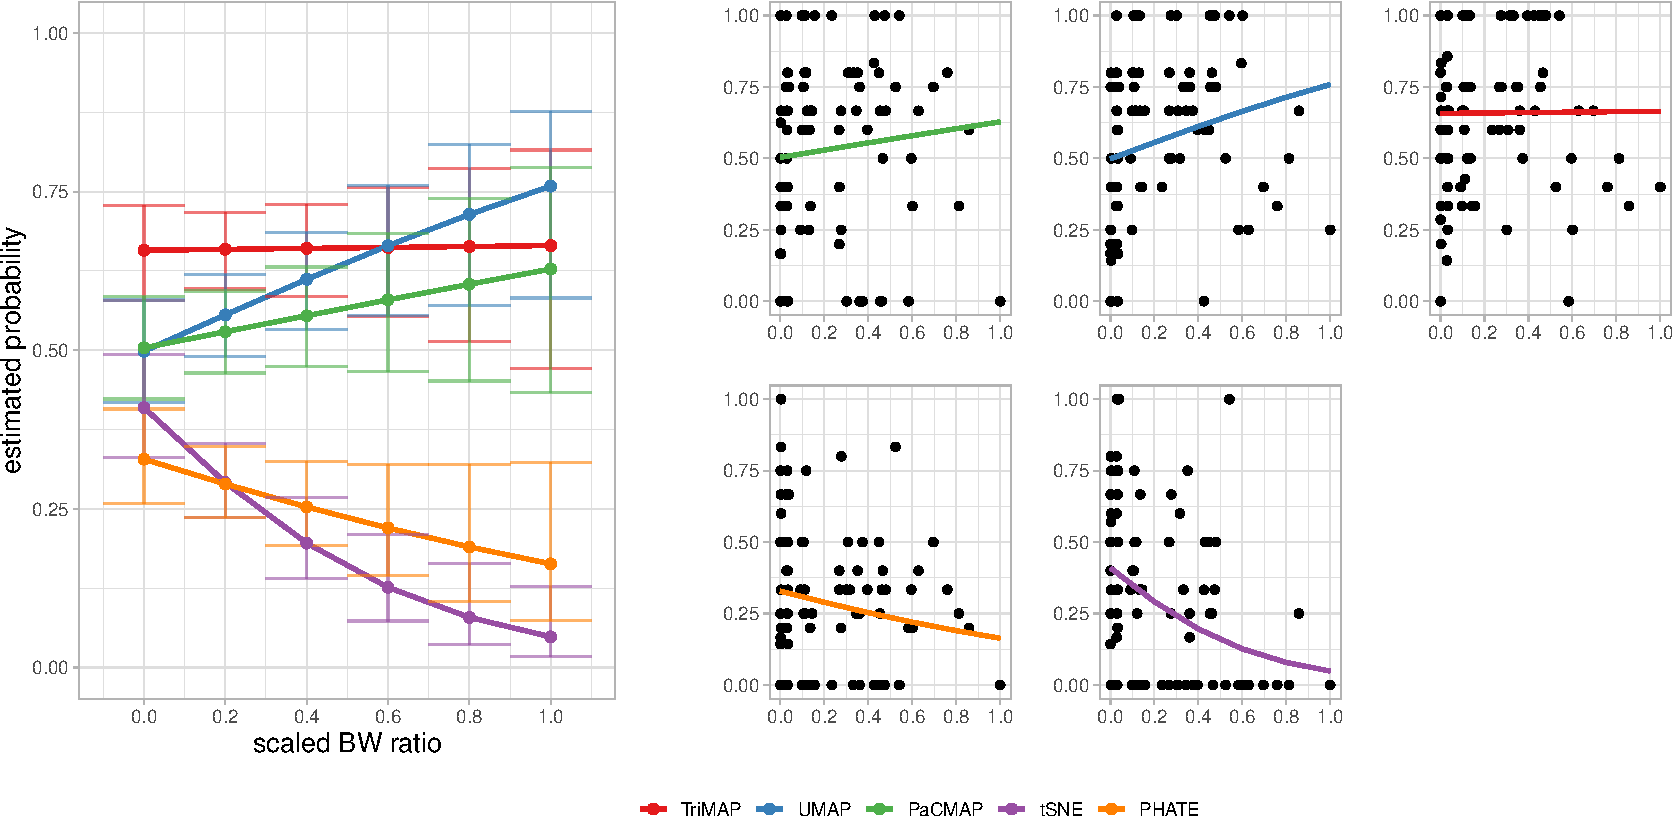
\includegraphics[width=1\linewidth,height=\textheight,keepaspectratio]{chapters/05-chap5_files/figure-pdf/fig-glmm-1.pdf}

}

\caption{\label{fig-glmm}Estimated probability of correctly identifying
the true cluster structure across different values of the scaled BW
ratio for five NLDR methods: TriMAP, UMAP, PaCMAP, tSNE, and PHATE. The
left panel shows the estimated probabilities and associated standard
errors across scaled BW ratio values. The right panels display the
observed probabilities of correct identification (black dots), along
with fitted logistic regression lines for each method. The scaled BW
ratio quantifies the relative separation between clusters, with higher
values indicating more distinct clustering. UMAP and PaCMAP show
increased accuracy with higher BW ratios, while tSNE, and PHATE decline
in performance. TriMAP remains stable across the range.}

\end{figure}%

Similarly, the model using exp(scaled minimum distance)
(Table~\ref{tbl-glmm-min}) confirms these trends
(Figure~\ref{fig-glmm-min}). Higher values of exp(scaled minimum
distance), representing greater spatial separation between clusters, are
associated with improved correctness for \emph{UMAP} and \emph{PaCMAP}.
In contrast, \emph{tSNE} and \emph{PHATE} again show a negative
association with increasing separation, while \emph{TriMAP} exhibits
consistent performance. These patterns suggest that the relative cluster
separability---whether quantified by BW ratio or minimum
distance---plays a crucial role in how well NLDR methods reveal the
underlying structure.

\begin{table}

\caption{\label{tbl-glmm-min}Logistic regression model results for
correct identification probability as a function of exp(scaled minimum
distance) and NLDR method (TriMAP as baseline). The table shows
estimates, standard errors, test statistics, and \emph{p}-values for
main effects and interactions. Significant positive associations with
exp(scaled minimum distance) indicate improved correctness with greater
cluster separation, while negative associations suggest reduced clarity.
Significance codes: (\(\emph{p}\leq 0.001\) `\texttt{***}',
\(\emph{p}\leq 0.01\) `\texttt{**}', \(\emph{p}\leq 0.05\) `\texttt{*}',
\(\emph{p}\leq 0.1\) `\texttt{.}').}

\centering{

\centering
\resizebox{\ifdim\width>\linewidth\linewidth\else\width\fi}{!}{
\begin{tabular}{lrrrrl}
\toprule
term & estimate & std.error & statistic & p.value & p\_val\_sig\\
\midrule
(Intercept) & 0.36 & 0.34 & 1.08 & 0.28 & \\
methodUMAP & -1.03 & 0.45 & -2.28 & 0.02 & *\\
methodPaCMAP & -0.57 & 0.45 & -1.27 & 0.20 & \\
methodtSNE & -0.03 & 0.47 & -0.07 & 0.95 & \\
methodPHATE & -0.73 & 0.47 & -1.56 & 0.12 & \\
exp\_min\_dist\_scaled & 0.20 & 0.20 & 0.97 & 0.33 & \\
methodUMAP:exp\_min\_dist\_scaled & 0.39 & 0.28 & 1.41 & 0.16 & \\
methodPaCMAP:exp\_min\_dist\_scaled & 0.02 & 0.28 & 0.08 & 0.94 & \\
methodtSNE:exp\_min\_dist\_scaled & -0.97 & 0.29 & -3.32 & 0.00 & ***\\
methodPHATE:exp\_min\_dist\_scaled & -0.55 & 0.29 & -1.90 & 0.06 & .\\
\bottomrule
\end{tabular}}

}

\end{table}%

\begin{figure}[H]

\centering{

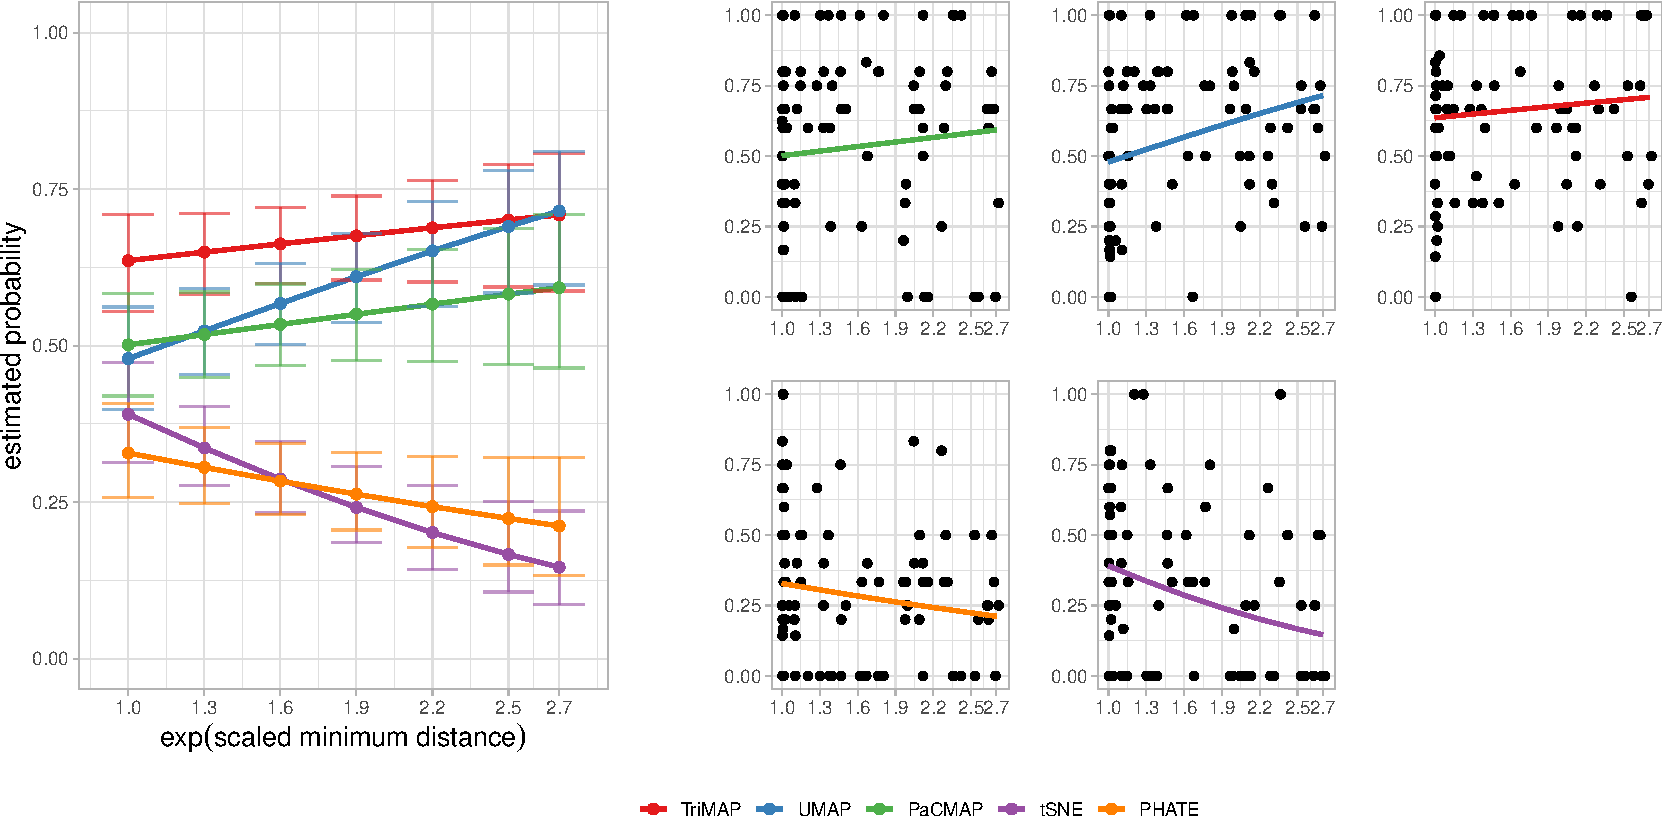
\includegraphics[width=1\linewidth,height=\textheight,keepaspectratio]{chapters/05-chap5_files/figure-pdf/fig-glmm-min-1.pdf}

}

\caption{\label{fig-glmm-min}Estimated probability of correctly
identifying the true cluster structure across different values of the
exp(scaled minimum distance) for five NLDR methods: TriMAP, UMAP,
PaCMAP, tSNE, and PHATE. The left panel shows the estimated
probabilities and associated standard errors across exp(scaled minimum
distance) values. The right panels display the observed probabilities of
correct identification (black dots), along with fitted logistic
regression lines for each method. The exp(scaled minimum distance)
quantifies the relative separation between clusters, with higher values
indicating more distinct clustering. UMAP and PaCMAP show increased
accuracy with higher minimum distances, while tSNE, and PHATE declines
in performance. TriMAP remains stable across the range.}

\end{figure}%

Together, these results highlight that \textbf{UMAP and PaCMAP are more
sensitive to improvements in cluster separation}, achieving higher
correct proportions as inter-cluster distances increase. Conversely,
\emph{tSNE} and \emph{PHATE} may lose fidelity in scenarios with very
distinct clusters, potentially due to their optimization dynamics.
\emph{TriMAP}'s consistent accuracy across distance scales reinforces
its stability and balanced preservation of local and global structure.

\subsection{Reasons for mis-identification by
method}\label{reasons-for-mis-identification-by-method}

Understanding why participants misidentified certain data structures
provides deeper insight into the perceptual consequences of each NLDR
method's underlying optimization principles. Each method uses a
different objective function to balance local and global structure
preservation, which can influence how faithfully high-dimensional
relationships are represented in \gD{}. To explore these differences, we
analyzed misidentifications across methods, identifying where and how
each algorithm tended to distort or merge clusters. This analysis
highlights systematic weaknesses linked to each method's design, helping
explain why some embeddings were more difficult for participants to
interpret correctly.

\subsubsection{TriMAP}\label{trimap}

TriMAP minimizes a triplet-based loss function that seeks to preserve
relative distances among triplets of points in \pD{} (Amid and Warmuth
(\citeproc{ref-amid2022}{2022})). This design emphasizes maintaining
global relationships between clusters but can underrepresent local
curvature and fine-scale geometry, particularly when clusters differ in
density or shape.

Figure~\ref{fig-mis-trimap} illustrates the two three-cluster data
structures that were most frequently misidentified when visualized using
TriMAP:
\emph{nonlinear\_hyperbola2--hemisphere--pyramid\_triangular\_base}
(three\_clust\_07) and
\emph{nonlinear\_hyperbola--elliptical--pyramid\_rectangular\_base}
(three\_clust\_15). In both cases, the underlying cluster separation
evident in \pD{} was not well preserved in the \gD{} NLDR layout.

Across these examples, TriMAP tends to merge neighboring clusters or
distort curved manifolds, leading to overlaps between nonlinear and
compact components such as \emph{elliptical} or \emph{pyramid}-shaped
clusters. The algorithm's emphasis on maintaining global relationships
can inadvertently compress local structure, particularly when manifolds
differ in curvature or density.

This projection bias results in flattened or partially merged
representations, where the curved components (e.g.,
\emph{nonlinear\_hyperbola}) lose their geometric integrity.
Consequently, TriMAP's performance declines when the data structure
involves a combination of curvilinear and planar clusters, revealing its
sensitivity to differences in shape complexity and scale.

\begin{figure}

\centering{

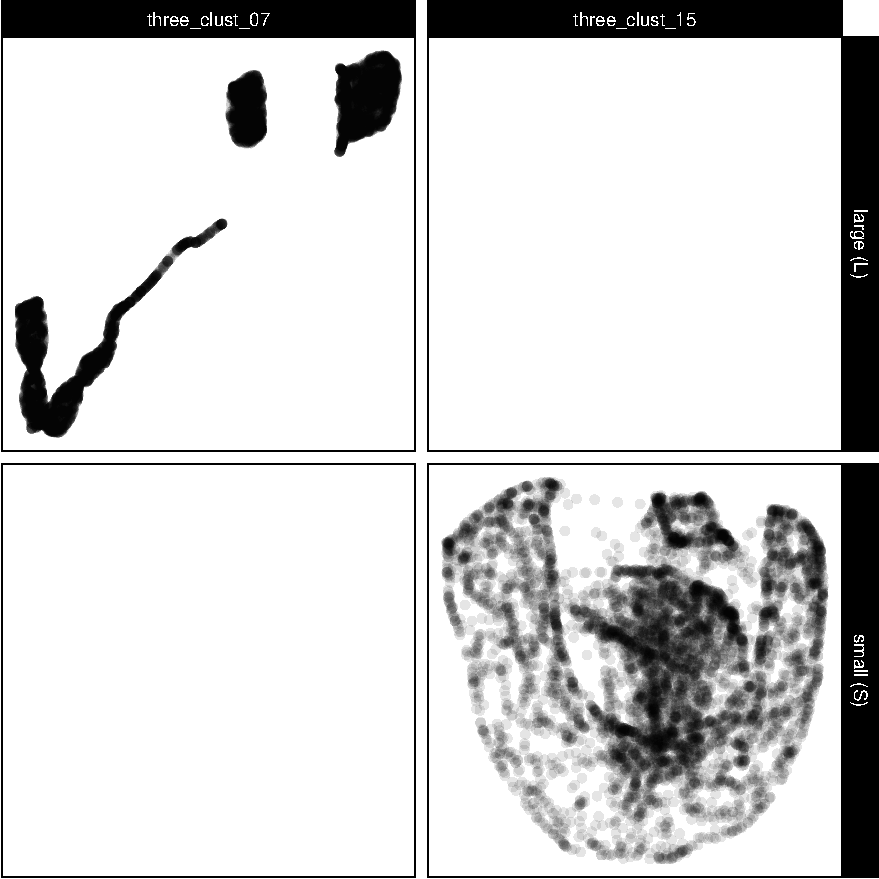
\includegraphics[width=1\linewidth,height=\textheight,keepaspectratio]{chapters/05-chap5_files/figure-pdf/fig-mis-trimap-1.pdf}

}

\caption{\label{fig-mis-trimap}TriMAP misidentifications for selected
three-cluster data structures. Each column corresponds to one data
structure, and each row shows the resulting \gD{} NLDR layout under
different distance scale settings: (a) small (S) and (b) large (L).
TriMAP often merges clusters or distorts their geometric boundaries,
particularly when the data include both compact and curved components.
This reflects the method's difficulty in preserving manifold curvature
and relative distances among clusters with differing density or shape.}

\end{figure}%

\begin{table}
\centering
\resizebox{\ifdim\width>\linewidth\linewidth\else\width\fi}{!}{
\begin{tabular}{lllll}
\toprule
data\_structure & cluster1 & cluster2 & cluster3 & distance\_sf\\
\midrule
three\_clust\_07 & nonlinear\_hyperbola2 & hemisphere & pyramid\_triangular\_base & large (L)\\
three\_clust\_15 & nonlinear\_hyperbola & elliptical & pyramid\_rectangular\_base & small (S)\\
\bottomrule
\end{tabular}}
\end{table}

\subsubsection{UMAP}\label{umap}

UMAP optimizes a cross-entropy loss between high- and low-dimensional
fuzzy simplicial sets (McInnes et al.
(\citeproc{ref-leland2018}{2018})). Its hyper-parameters---n\_neighbors
and min\_dist---govern the trade-off between local and global structure.

Figure~\ref{fig-mis-umap} presents the three-cluster data structures
that were misidentified by UMAP. The corresponding true high-dimensional
structures are \emph{s\_curve--cube--pyramid\_rectangular\_base}
(three\_clust\_02),
\emph{nonlinear\_hyperbola--elliptical--blunted\_cone}
(three\_clust\_05), \emph{helical\_hyper\_spiral--cube--blunted\_cone}
(three\_clust\_09), and \emph{curvy\_cylinder--cube--blunted\_cone}
(three\_clust\_13).

UMAP demonstrates partial success in separating clusters but exhibits
notable distortions in geometric structure and merging of neighboring
clusters in several cases. For instance, in three\_clust\_02 and
three\_clust\_09, curved manifolds (s\_curve and helical\_hyper\_spiral)
are projected into compact or fragmented \gD{} regions, reducing the
apparent curvature and continuity of the original structure. In
three\_clust\_05 and three\_clust\_13, UMAP tends to merge blunted\_cone
and elliptical or cube clusters, suggesting difficulty in maintaining
separation between clusters of different densities or similar central
positions in the high-dimensional space.

These results indicate that while UMAP is generally effective at
maintaining local neighborhood relationships, it can fail to preserve
global geometry when clusters differ in shape or scale. The observed
misidentifications likely arise from its default parameterization, where
a small min\_dist and moderate n\_neighbors emphasize local compactness
at the expense of broader structural fidelity.

\begin{figure}

\centering{

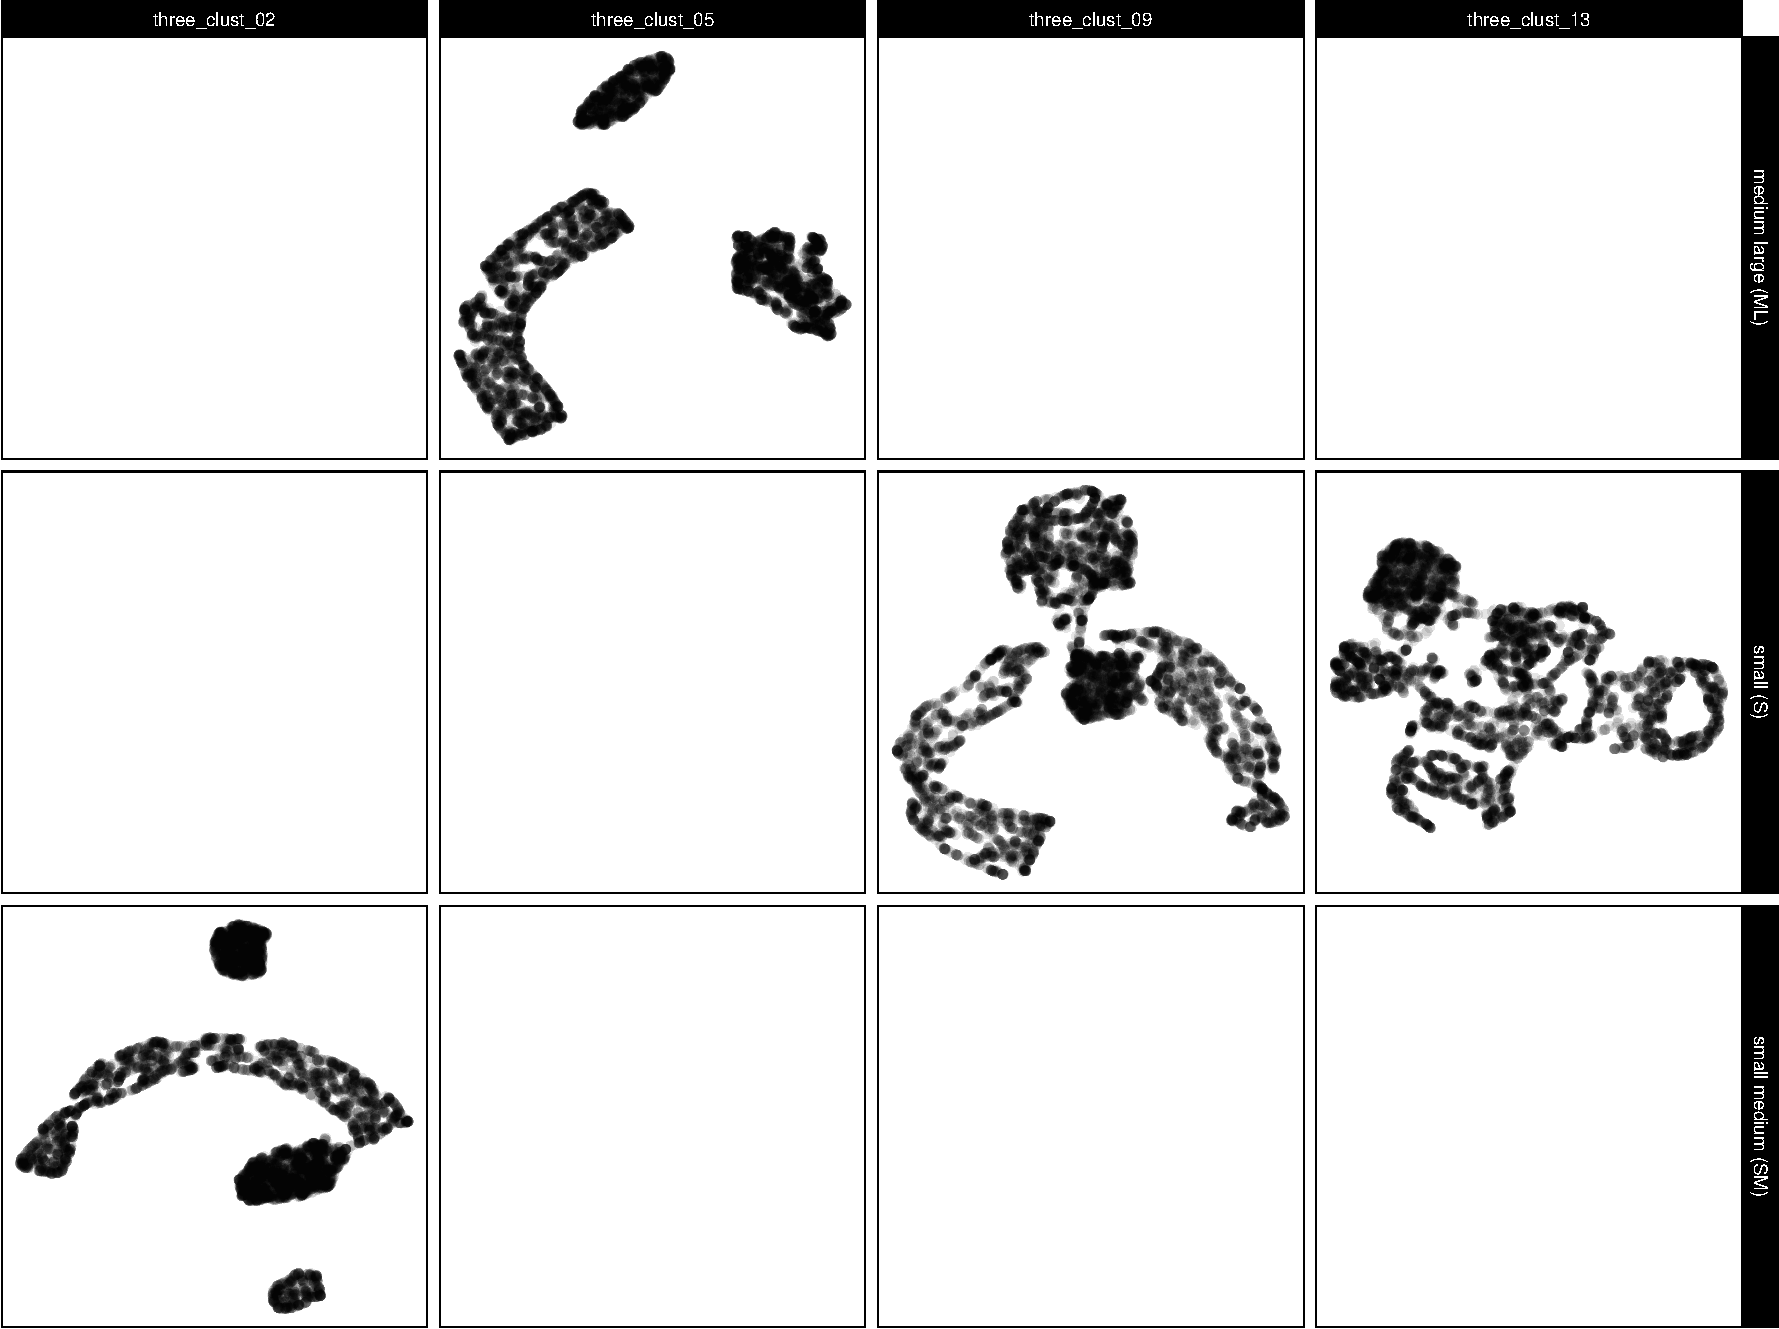
\includegraphics[width=1\linewidth,height=\textheight,keepaspectratio]{chapters/05-chap5_files/figure-pdf/fig-mis-umap-1.pdf}

}

\caption{\label{fig-mis-umap}UMAP misidentifications for selected
three-cluster data structures. Each column corresponds to one data
structure, and each row shows the resulting \gD{} NLDR layout under
different distance scale settings: (a) small (S), (b) small medium (SM),
and (c) medium large (ML). UMAP often merges clusters or distorts curved
manifolds, particularly when clusters differ in geometric complexity or
density.}

\end{figure}%

\begin{table}
\centering
\resizebox{\ifdim\width>\linewidth\linewidth\else\width\fi}{!}{
\begin{tabular}{lllll}
\toprule
data\_structure & cluster1 & cluster2 & cluster3 & distance\_sf\\
\midrule
three\_clust\_02 & s\_curve & cube & pyramid\_rectangular\_base & small medium (SM)\\
three\_clust\_05 & nonlinear\_hyperbola & elliptical & blunted\_cone & medium large (ML)\\
three\_clust\_09 & helical\_hyper\_spiral & cube & blunted\_cone & small (S)\\
three\_clust\_13 & curvy\_cylinder & cube & blunted\_cone & small (S)\\
\bottomrule
\end{tabular}}
\end{table}

\subsubsection{PaCMAP}\label{pacmap}

PaCMAP uses a multi-term objective combining near, mid-range, and
further pair constraints (Wang et al.
(\citeproc{ref-yingfan2021}{2021})), designed to improve global
structure compared to tSNE and UMAP.

Figure~\ref{fig-mis-pacmap} displays the data structures for which
PaCMAP produced notable misidentifications in the \gD{} embedding. The
true high-dimensional configurations for these datasets include
\emph{s\_curve--cube--pyramid\_rectangular\_base} (three\_clust\_02),
\emph{curvy\_cylinder--hemisphere--pyramid\_triangular\_base}
(three\_clust\_03), \emph{crescent--cube--pyramid\_rectangular\_base}
(three\_clust\_06),
\emph{nonlinear\_hyperbola2--hemisphere--pyramid\_triangular\_base}
(three\_clust\_07), \emph{helical\_hyper\_spiral--cube--blunted\_cone}
(three\_clust\_09),
\emph{spherical\_spiral--gaussian--pyramid\_triangular\_base}
(three\_clust\_10), \emph{curvy\_cylinder--cube--blunted\_cone}
(three\_clust\_13),
\emph{nonlinear\_hyperbola--elliptical--pyramid\_rectangular\_base}
(three\_clust\_15), and
\emph{nonlinear\_hyperbola2--cube--blunted\_cone} (three\_clust\_17).

Across these examples, PaCMAP tends to preserve local density structure
within clusters effectively but often struggles with global positioning
and relative orientation among clusters. For example, in
three\_clust\_02, the s\_curve and cube clusters remain relatively
well-formed but are positioned too close to the
pyramid\_rectangular\_base cluster, creating apparent overlaps.
Similarly, in three\_clust\_06 and three\_clust\_07, the pyramid-shaped
clusters are fragmented into smaller subgroups, suggesting instability
in maintaining global manifold continuity.

A consistent observation is that PaCMAP compresses or folds curved or
elongated manifolds, such as s\_curve, helical\_hyper\_spiral, and
nonlinear\_hyperbola2, into smaller regions of the \gD{} space. This
distortion likely arises from the algorithm's use of both near and
mid-range neighbor preservation terms, which balance local and global
structure but can underrepresent nonlinear curvature when clusters vary
in geometric complexity or density.

Overall, these results indicate that PaCMAP achieves visually clean
separation for simpler or isotropic clusters but tends to overcompress
nonlinearly extended clusters and misplace asymmetric shapes, resulting
in inaccurate global relationships between clusters.

\begin{figure}

\centering{

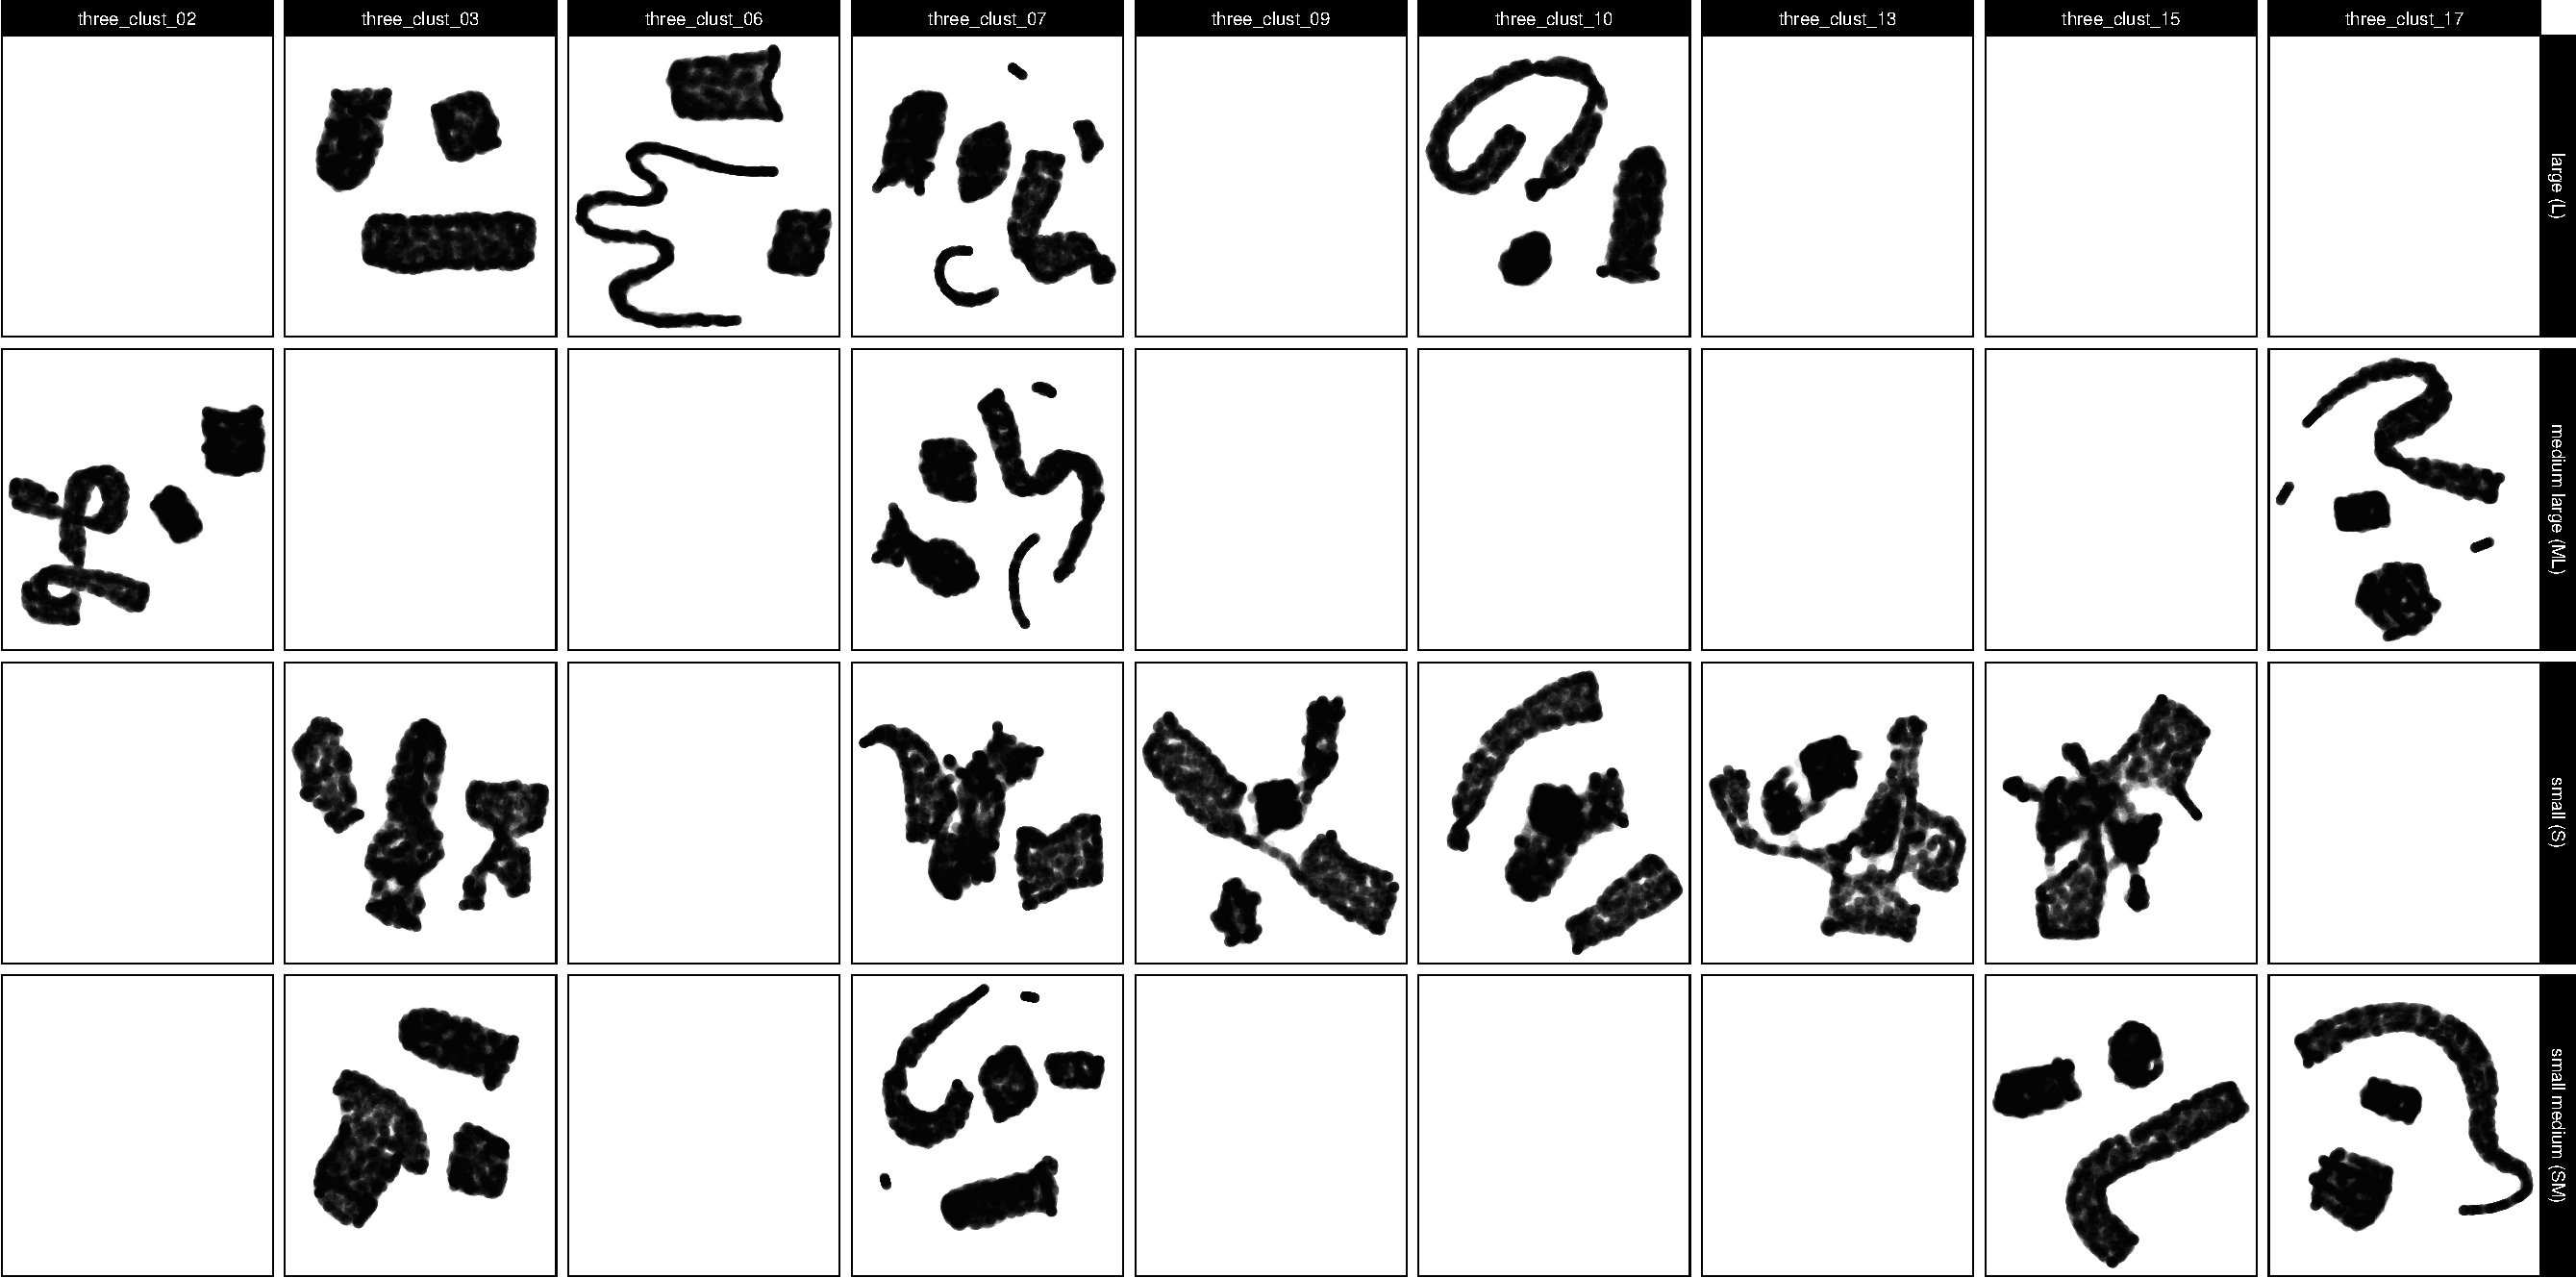
\includegraphics[width=1\linewidth,height=\textheight,keepaspectratio]{chapters/05-chap5_files/figure-pdf/fig-mis-pacmap-1.pdf}

}

\caption{\label{fig-mis-pacmap}PaCMAP misidentifications for selected
three-cluster data structures. Each column represents a distinct
high-dimensional data structure, while each row corresponds to a
resulting \gD{} NLDR layout under different distance scale settings: (a)
small (S), (b) small medium (SM), (c) medium large (ML), and (d) large
(L). PaCMAP effectively maintains intra-cluster cohesion but often
distorts the relative geometry between curved and compact clusters,
leading to apparent overlaps or misplacement in \gD{} space.}

\end{figure}%

\begin{table}
\centering
\resizebox{\ifdim\width>\linewidth\linewidth\else\width\fi}{!}{
\begin{tabular}{lllll}
\toprule
data\_structure & cluster1 & cluster2 & cluster3 & distance\_sf\\
\midrule
three\_clust\_02 & s\_curve & cube & pyramid\_rectangular\_base & medium large (ML)\\
three\_clust\_03 & curvy\_cylinder & hemisphere & pyramid\_triangular\_base & small (S)\\
three\_clust\_03 & curvy\_cylinder & hemisphere & pyramid\_triangular\_base & small medium (SM)\\
three\_clust\_03 & curvy\_cylinder & hemisphere & pyramid\_triangular\_base & large (L)\\
three\_clust\_06 & crescent & cube & pyramid\_rectangular\_base & large (L)\\
three\_clust\_07 & nonlinear\_hyperbola2 & hemisphere & pyramid\_triangular\_base & small (S)\\
three\_clust\_07 & nonlinear\_hyperbola2 & hemisphere & pyramid\_triangular\_base & small medium (SM)\\
three\_clust\_07 & nonlinear\_hyperbola2 & hemisphere & pyramid\_triangular\_base & medium large (ML)\\
three\_clust\_07 & nonlinear\_hyperbola2 & hemisphere & pyramid\_triangular\_base & large (L)\\
three\_clust\_09 & helical\_hyper\_spiral & cube & blunted\_cone & small (S)\\
three\_clust\_10 & spherical\_spiral & gaussian & pyramid\_triangular\_base & small (S)\\
three\_clust\_10 & spherical\_spiral & gaussian & pyramid\_triangular\_base & large (L)\\
three\_clust\_13 & curvy\_cylinder & cube & blunted\_cone & small (S)\\
three\_clust\_15 & nonlinear\_hyperbola & elliptical & pyramid\_rectangular\_base & small (S)\\
three\_clust\_15 & nonlinear\_hyperbola & elliptical & pyramid\_rectangular\_base & small medium (SM)\\
three\_clust\_17 & nonlinear\_hyperbola2 & cube & blunted\_cone & small medium (SM)\\
three\_clust\_17 & nonlinear\_hyperbola2 & cube & blunted\_cone & medium large (ML)\\
\bottomrule
\end{tabular}}
\end{table}

\subsubsection{tSNE}\label{tsne}

tSNE minimizes the Kullback--Leibler (KL) divergence between pairwise
similarities in high and low dimensions (Maaten and Hinton
(\citeproc{ref-laurens2008}{2008})). This objective strongly prioritizes
local neighborhood preservation while ignoring global distances.

Figure~\ref{fig-mis-tsne} illustrates the data structures where tSNE
produced misidentifications or distortions in the \gD{} embedding. The
affected datasets include
\emph{s\_curve--cube--pyramid\_rectangular\_base} (three\_clust\_02),
\emph{curvy\_cylinder--hemisphere--pyramid\_triangular\_base}
(three\_clust\_03), \emph{curv2--gaussian--filled\_hexagonal\_pyramid}
(three\_clust\_04),
\emph{nonlinear\_hyperbola--elliptical--blunted\_cone}
(three\_clust\_05), \emph{crescent--cube--pyramid\_rectangular\_base}
(three\_clust\_06),
\emph{nonlinear\_hyperbola2--hemisphere--pyramid\_triangular\_base}
(three\_clust\_07),
\emph{conic\_spiral--gaussian--filled\_hexagonal\_pyramid}
(three\_clust\_08), \emph{helical\_hyper\_spiral--cube--blunted\_cone}
(three\_clust\_09),
\emph{spherical\_spiral--gaussian--pyramid\_triangular\_base}
(three\_clust\_10),
\emph{s\_curve--hemisphere--filled\_hexagonal\_pyramid}
(three\_clust\_12), \emph{curv2--gaussian--pyramid\_triangular\_base}
(three\_clust\_14),
\emph{nonlinear\_hyperbola--elliptical--pyramid\_rectangular\_base}
(three\_clust\_15),
\emph{crescent--hemisphere--filled\_hexagonal\_pyramid}
(three\_clust\_16), \emph{nonlinear\_hyperbola2--cube--blunted\_cone}
(three\_clust\_17), and
\emph{conic\_spiral--gaussian--pyramid\_triangular\_base}
(three\_clust\_18).

Across these examples, tSNE successfully captures local structure within
clusters---preserving compactness and density---but often fails to
represent the global arrangement among multiple clusters. In several
cases, tSNE artificially amplifies distances between geometrically
related clusters (e.g., s\_curve and cube in three\_clust\_02) or splits
continuous manifolds such as nonlinear\_hyperbola and
helical\_hyper\_spiral into disjoint fragments. This fragmentation
suggests that tSNE's heavy emphasis on preserving local neighborhoods
comes at the cost of losing the true topological continuity of
non-linear shapes.

A recurring issue is that tSNE tends to over-separate clusters when they
differ in density or curvature. For instance, in three\_clust\_06 and
three\_clust\_07, one or more clusters (particularly those with curved
or open structures) are pushed disproportionately far apart, producing
an embedding that exaggerates separation. Additionally, tSNE appears
sensitive to cluster anisotropy---for example, pyramid\_triangular\_base
and filled\_hexagonal\_pyramid clusters often appear distorted or
collapsed into compact forms, suggesting that their high-dimensional
shape complexity is not faithfully maintained in the low-dimensional
layout.

Overall, these misidentifications reveal that while tSNE produces
visually distinct clusters with strong local cohesion, it frequently
distorts global geometry, particularly when clusters vary in curvature,
scale, or orientation.

\begin{figure}

\centering{

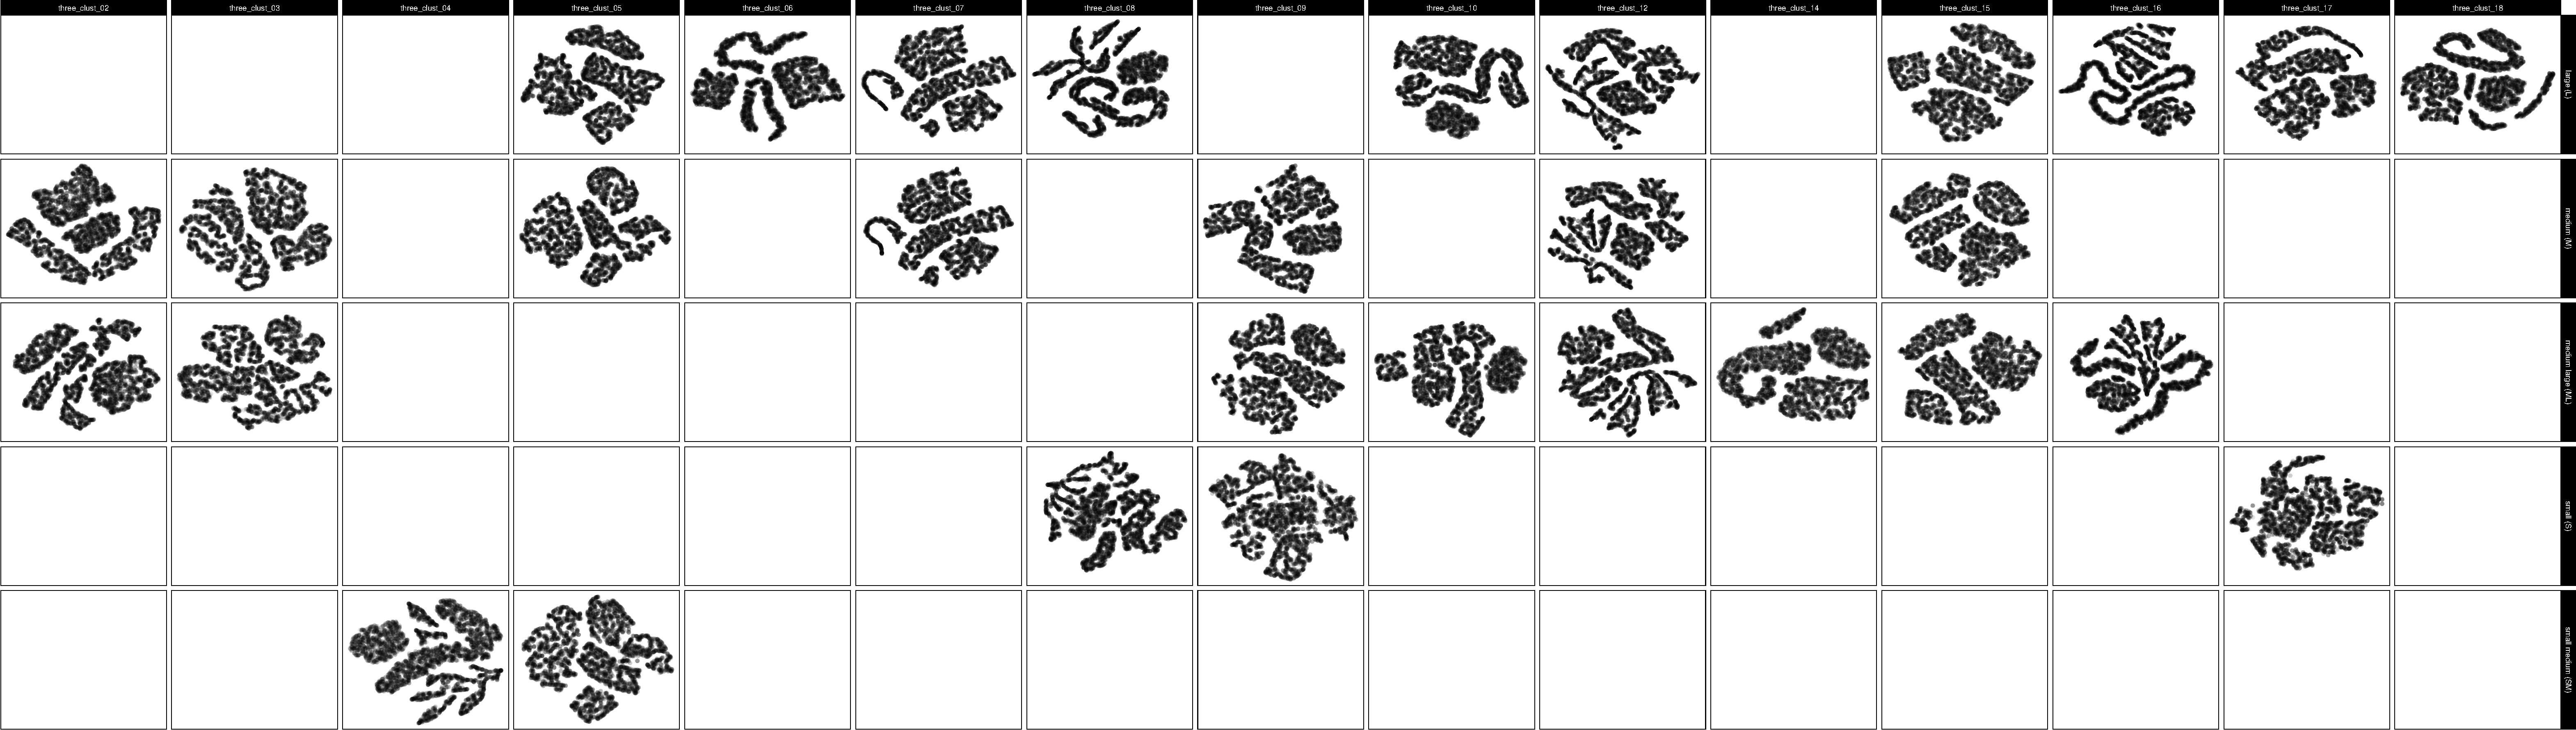
\includegraphics[width=1\linewidth,height=\textheight,keepaspectratio]{chapters/05-chap5_files/figure-pdf/fig-mis-tsne-1.pdf}

}

\caption{\label{fig-mis-tsne}tSNE misidentifications for selected
three-cluster data structures. Each column represents a distinct
high-dimensional data structure, while each row corresponds to a
resulting \gD{} NLDR layout under different distance scale settings: (a)
small (S), (b) small medium (SM), (c) medium (M), (d) medium large (ML),
and (e) large (L). tSNE effectively maintains within-cluster density and
separation but tends to distort the global spatial relationships among
clusters---especially when the data include non-linear or anisotropic
geometries such as hyperbolas, spirals, and pyramids.}

\end{figure}%

\begin{table}
\centering
\resizebox{\ifdim\width>\linewidth\linewidth\else\width\fi}{!}{
\begin{tabular}{lllll}
\toprule
data\_structure & cluster1 & cluster2 & cluster3 & distance\_sf\\
\midrule
three\_clust\_02 & s\_curve & cube & pyramid\_rectangular\_base & medium (M)\\
three\_clust\_02 & s\_curve & cube & pyramid\_rectangular\_base & medium large (ML)\\
three\_clust\_03 & curvy\_cylinder & hemisphere & pyramid\_triangular\_base & medium (M)\\
three\_clust\_03 & curvy\_cylinder & hemisphere & pyramid\_triangular\_base & medium large (ML)\\
three\_clust\_04 & curv2 & gaussian & filled\_hexagonal\_pyramid & small medium (SM)\\
three\_clust\_05 & nonlinear\_hyperbola & elliptical & blunted\_cone & small medium (SM)\\
three\_clust\_05 & nonlinear\_hyperbola & elliptical & blunted\_cone & medium (M)\\
three\_clust\_05 & nonlinear\_hyperbola & elliptical & blunted\_cone & large (L)\\
three\_clust\_06 & crescent & cube & pyramid\_rectangular\_base & large (L)\\
three\_clust\_07 & nonlinear\_hyperbola2 & hemisphere & pyramid\_triangular\_base & medium (M)\\
three\_clust\_07 & nonlinear\_hyperbola2 & hemisphere & pyramid\_triangular\_base & large (L)\\
three\_clust\_08 & conic\_spiral & gaussian & filled\_hexagonal\_pyramid & small (S)\\
three\_clust\_08 & conic\_spiral & gaussian & filled\_hexagonal\_pyramid & large (L)\\
three\_clust\_09 & helical\_hyper\_spiral & cube & blunted\_cone & small (S)\\
three\_clust\_09 & helical\_hyper\_spiral & cube & blunted\_cone & medium (M)\\
three\_clust\_09 & helical\_hyper\_spiral & cube & blunted\_cone & medium large (ML)\\
three\_clust\_10 & spherical\_spiral & gaussian & pyramid\_triangular\_base & medium large (ML)\\
three\_clust\_10 & spherical\_spiral & gaussian & pyramid\_triangular\_base & large (L)\\
three\_clust\_12 & s\_curve & hemisphere & filled\_hexagonal\_pyramid & medium (M)\\
three\_clust\_12 & s\_curve & hemisphere & filled\_hexagonal\_pyramid & medium large (ML)\\
three\_clust\_12 & s\_curve & hemisphere & filled\_hexagonal\_pyramid & large (L)\\
three\_clust\_14 & curv2 & gaussian & pyramid\_triangular\_base & medium large (ML)\\
three\_clust\_15 & nonlinear\_hyperbola & elliptical & pyramid\_rectangular\_base & medium (M)\\
three\_clust\_15 & nonlinear\_hyperbola & elliptical & pyramid\_rectangular\_base & medium large (ML)\\
three\_clust\_15 & nonlinear\_hyperbola & elliptical & pyramid\_rectangular\_base & large (L)\\
three\_clust\_16 & crescent & hemisphere & filled\_hexagonal\_pyramid & medium large (ML)\\
three\_clust\_16 & crescent & hemisphere & filled\_hexagonal\_pyramid & large (L)\\
three\_clust\_17 & nonlinear\_hyperbola2 & cube & blunted\_cone & small (S)\\
three\_clust\_17 & nonlinear\_hyperbola2 & cube & blunted\_cone & large (L)\\
three\_clust\_18 & conic\_spiral & gaussian & pyramid\_triangular\_base & large (L)\\
\bottomrule
\end{tabular}}
\end{table}

\subsubsection{PHATE}\label{phate}

PHATE constructs a diffusion-based potential distance that encodes
multi-scale manifold structure (Moon et al.
(\citeproc{ref-moon2019}{2019})). This approach excels at capturing
continuous transitions, but tends to over-smooth boundaries between
discrete clusters.

Figure~\ref{fig-mis-phate} presents the high-dimensional data structures
for which PHATE led to misidentification or structural distortion in the
\gD{} embedding. The affected datasets include
\emph{curv--elliptical--blunted\_cone} (three\_clust\_01),
\emph{s\_curve--cube--pyramid\_rectangular\_base} (three\_clust\_02),
curvy\_cylinder--hemisphere--pyramid\_triangular\_base
(three\_clust\_03), \emph{curv2--gaussian--filled\_hexagonal\_pyramid}
(three\_clust\_04),
\emph{nonlinear\_hyperbola--elliptical--blunted\_cone}
(three\_clust\_05), \emph{crescent--cube--pyramid\_rectangular\_base}
(three\_clust\_06),
\emph{nonlinear\_hyperbola2--hemisphere--pyramid\_triangular\_base}
(three\_clust\_07),
\emph{conic\_spiral--gaussian--filled\_hexagonal\_pyramid}
(three\_clust\_08), \emph{helical\_hyper\_spiral--cube--blunted\_cone}
(three\_clust\_09),
\emph{spherical\_spiral--gaussian--pyramid\_triangular\_base}
(three\_clust\_10), \emph{curv--elliptical--pyramid\_rectangular\_base}
(three\_clust\_11),
\emph{s\_curve--hemisphere--filled\_hexagonal\_pyramid}
(three\_clust\_12), \emph{curvy\_cylinder--cube--blunted\_cone}
(three\_clust\_13), \emph{curv2--gaussian--pyramid\_triangular\_base}
(three\_clust\_14),
\emph{nonlinear\_hyperbola--elliptical--pyramid\_rectangular\_base}
(three\_clust\_15),
\emph{crescent--hemisphere--filled\_hexagonal\_pyramid}
(three\_clust\_16), and
\emph{conic\_spiral--gaussian--pyramid\_triangular\_base}
(three\_clust\_18).

PHATE tends to preserve smooth manifold continuity across most clusters
but exhibits misidentifications primarily when clusters differ in
geometric curvature or density. For instance, in structures such as
s\_curve--cube--pyramid\_rectangular\_base (three\_clust\_02) and
curvy\_cylinder--hemisphere--pyramid\_triangular\_base
(three\_clust\_03), PHATE partially merges distinct clusters along
gradual transitions, reflecting its tendency to emphasize global
manifold smoothness at the expense of discrete cluster separation. This
blending effect is especially evident when clusters possess shared
curvature characteristics, such as nonlinear\_hyperbola and
helical\_hyper\_spiral, or when the transition between shapes is
continuous in high-dimensional space.

Another recurring pattern involves shape compression, where complex
structures like filled\_hexagonal\_pyramid and pyramid\_triangular\_base
are collapsed into more isotropic forms. This occurs because PHATE's
diffusion-based approach tends to over-smooth distances, leading to
reduced contrast between dense and sparse regions. As a result, clusters
with sharp edges or hollow geometries (e.g., pyramidal or conical
shapes) lose their distinct form and may appear more circular in the
\gD{} embedding.

Overall, PHATE performs well in maintaining global topology and gradual
transitions, making it suitable for continuous manifolds such as
s\_curve or crescent. However, it struggles to preserve clear separation
among distinct, non-linear, or sharply bounded clusters, often blending
or distorting them when the high-dimensional geometry involves abrupt
curvature changes or contrasting densities.

\begin{figure}

\centering{

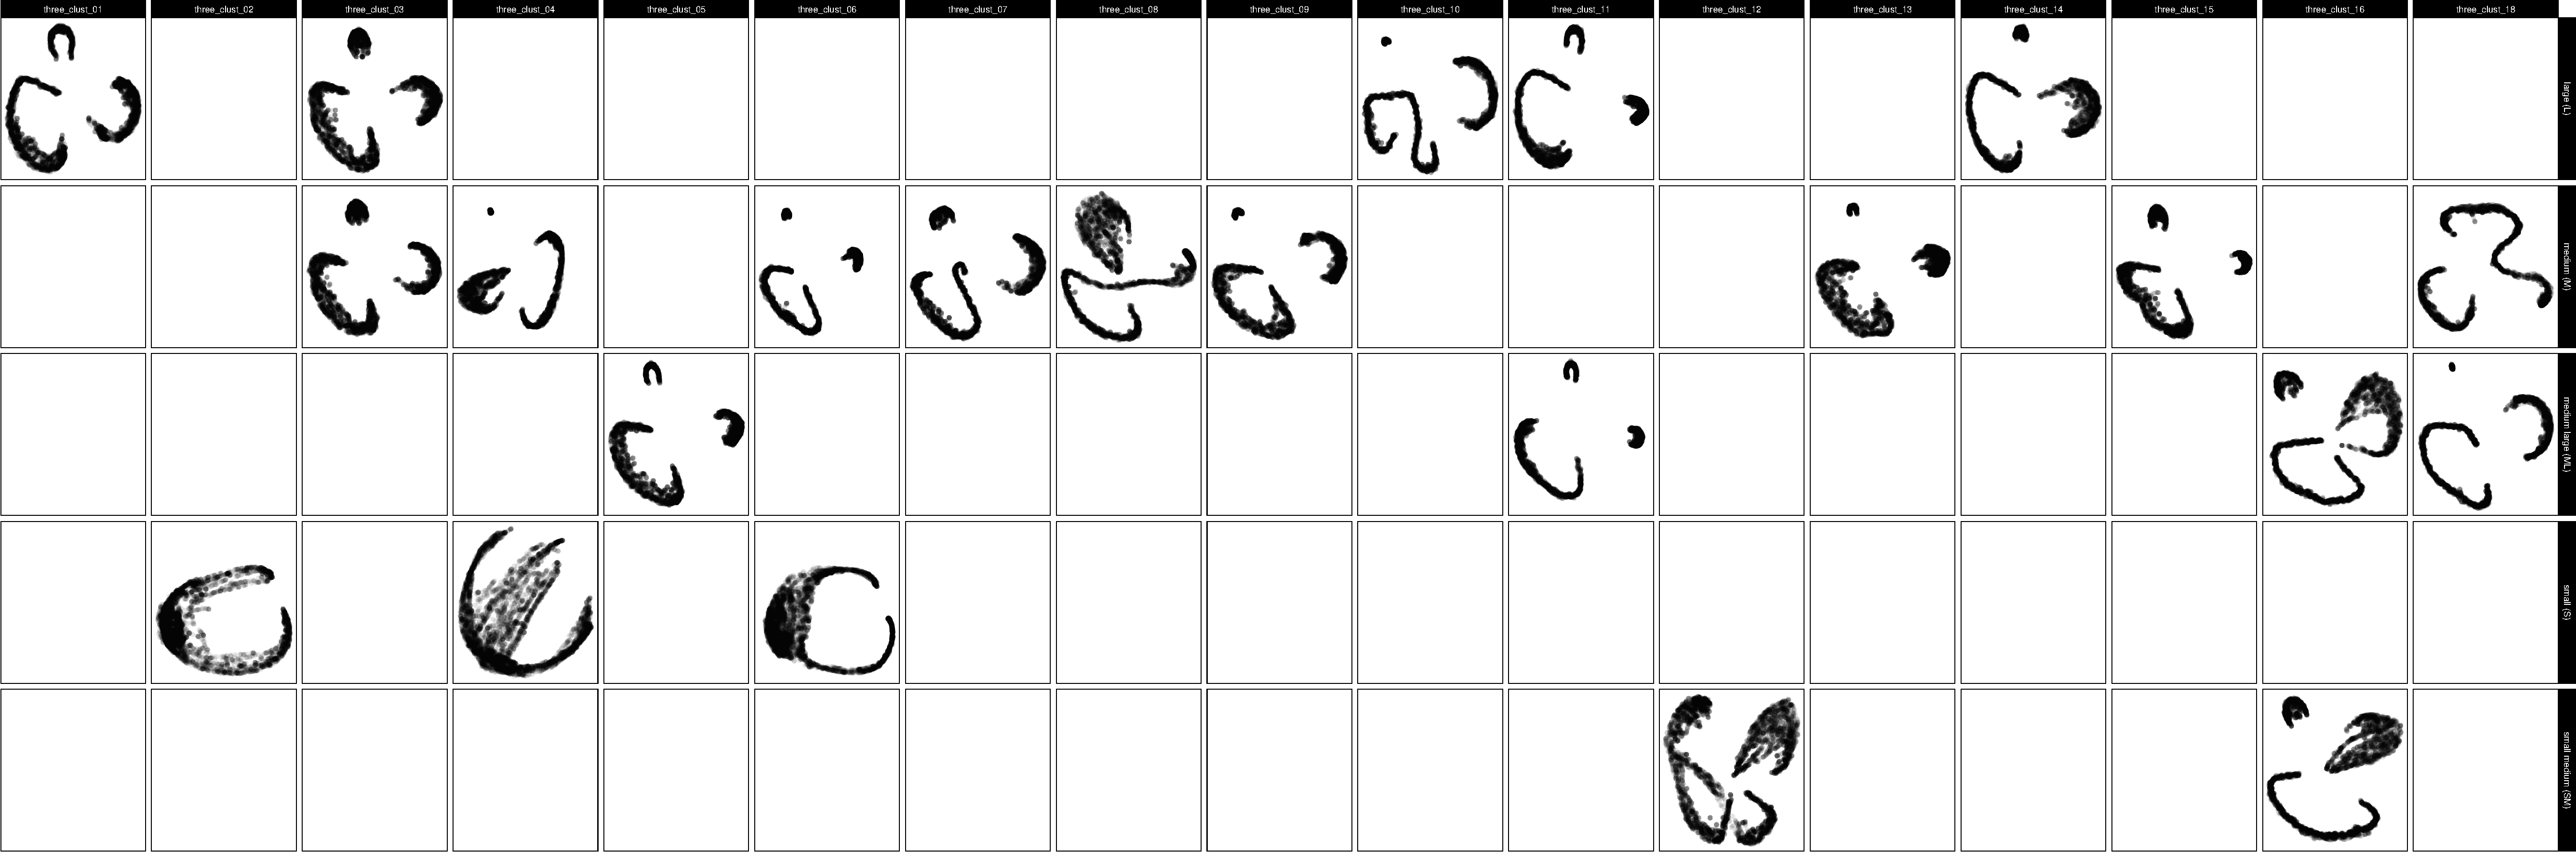
\includegraphics[width=1\linewidth,height=\textheight,keepaspectratio]{chapters/05-chap5_files/figure-pdf/fig-mis-phate-1.pdf}

}

\caption{\label{fig-mis-phate}PHATE misidentifications for selected
three-cluster data structures. Each column represents a distinct
high-dimensional data structure, while each row corresponds to a
resulting \gD{} NLDR layout under different distance scale settings: (a)
small (S), (b) small medium (SM), (c) medium (M), (d) medium large (ML),
and (e) large (L). PHATE effectively maintains global continuity but
exhibits over-smoothing, leading to partial merging or distortion of
geometrically distinct clusters---particularly for combinations
involving hyperbolas, pyramids, and cones.}

\end{figure}%

\begin{table}
\centering
\resizebox{\ifdim\width>\linewidth\linewidth\else\width\fi}{!}{
\begin{tabular}{lllll}
\toprule
data\_structure & cluster1 & cluster2 & cluster3 & distance\_sf\\
\midrule
three\_clust\_01 & curv & elliptical & blunted\_cone & large (L)\\
three\_clust\_02 & s\_curve & cube & pyramid\_rectangular\_base & small (S)\\
three\_clust\_03 & curvy\_cylinder & hemisphere & pyramid\_triangular\_base & medium (M)\\
three\_clust\_03 & curvy\_cylinder & hemisphere & pyramid\_triangular\_base & large (L)\\
three\_clust\_04 & curv2 & gaussian & filled\_hexagonal\_pyramid & small (S)\\
three\_clust\_04 & curv2 & gaussian & filled\_hexagonal\_pyramid & medium (M)\\
three\_clust\_05 & nonlinear\_hyperbola & elliptical & blunted\_cone & medium large (ML)\\
three\_clust\_06 & crescent & cube & pyramid\_rectangular\_base & small (S)\\
three\_clust\_06 & crescent & cube & pyramid\_rectangular\_base & medium (M)\\
three\_clust\_07 & nonlinear\_hyperbola2 & hemisphere & pyramid\_triangular\_base & medium (M)\\
three\_clust\_08 & conic\_spiral & gaussian & filled\_hexagonal\_pyramid & medium (M)\\
three\_clust\_09 & helical\_hyper\_spiral & cube & blunted\_cone & medium (M)\\
three\_clust\_10 & spherical\_spiral & gaussian & pyramid\_triangular\_base & large (L)\\
three\_clust\_11 & curv & elliptical & pyramid\_rectangular\_base & medium large (ML)\\
three\_clust\_11 & curv & elliptical & pyramid\_rectangular\_base & large (L)\\
three\_clust\_12 & s\_curve & hemisphere & filled\_hexagonal\_pyramid & small medium (SM)\\
three\_clust\_13 & curvy\_cylinder & cube & blunted\_cone & medium (M)\\
three\_clust\_14 & curv2 & gaussian & pyramid\_triangular\_base & large (L)\\
three\_clust\_15 & nonlinear\_hyperbola & elliptical & pyramid\_rectangular\_base & medium (M)\\
three\_clust\_16 & crescent & hemisphere & filled\_hexagonal\_pyramid & small medium (SM)\\
three\_clust\_16 & crescent & hemisphere & filled\_hexagonal\_pyramid & medium large (ML)\\
three\_clust\_18 & conic\_spiral & gaussian & pyramid\_triangular\_base & medium (M)\\
three\_clust\_18 & conic\_spiral & gaussian & pyramid\_triangular\_base & medium large (ML)\\
\bottomrule
\end{tabular}}
\end{table}

\subsection{Reasons for mis-identification by number of
component(s)}\label{reasons-for-mis-identification-by-number-of-components}

Beyond method-specific effects, the complexity of the high-dimensional
data itself also influenced recognition accuracy. Some
misidentifications involved confusion between a single cluster and
another, while others reflected blending or merging of multiple
clusters. To investigate these patterns, we categorized
misidentifications based on the number of cluster components
involved---one, two, or three---and visualized their intersections
across NLDR methods using UpSet plots. This analysis reveals how data
complexity interacts with embedding behavior, shedding light on whether
misidentification arises primarily from local distortions, partial
overlaps, or global structural confusion.

\subsubsection{One component}\label{one-component}

The first UpSet plot (Figure~\ref{fig-upset-one}) shows the
intersections of single-component misidentifications across methods.
Each horizontal bar represents the number of times a particular data
structure component was misidentified, and the vertical bars indicate
combinations of NLDR methods that shared the same misidentifications.

The most frequently co-misidentified structures across methods included
\emph{pyramid\_rectangular\_base, nonlinear\_hyperbola, elliptical,
s\_curve, pyramid\_triangular\_base, nonlinear\_hyperbola2, hemisphere,
helical\_hyper\_spiral, curvy\_cylinder, cube, blunted\_cone,
spherical\_spiral, gaussian, and crescent}.

These structures are geometrically curved, non-spherical, or
multi-surface, making them prone to distortion in \gD{} embeddings. For
instance, nonlinear\_hyperbola and s\_curve contain pronounced curvature
and variable density, which local-attraction methods like tSNE and PHATE
often compress unevenly. Similarly, pyramid\_rectangular\_base and
blunted\_cone exhibit mixed sharp and smooth edges, challenging methods
that rely on uniform neighborhood scaling.

Across methods, the greatest overlap occurred among PaCMAP, PHATE, tSNE,
and UMAP, all of which misidentified at least four of these structures.
TriMAP exhibited relatively fewer single-component errors, reflecting
its stronger preservation of global relationships.

\begin{figure}

\centering{

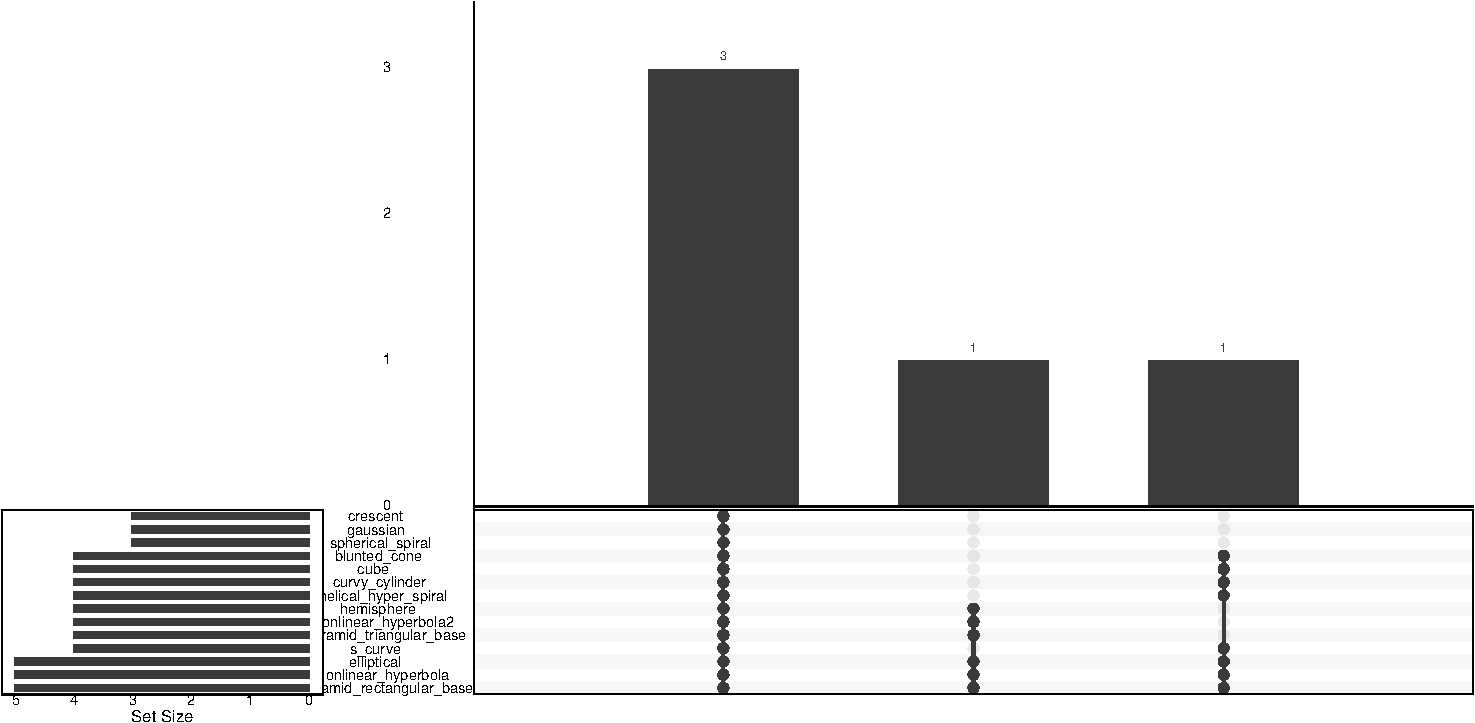
\includegraphics[width=1\linewidth,height=\textheight,keepaspectratio]{chapters/05-chap5_files/figure-pdf/fig-upset-one-1.pdf}

}

\caption{\label{fig-upset-one}UpSet plot showing intersections of
misidentified data structure components across NLDR methods. Each
horizontal bar on the left represents the number of times a particular
data structure component was misidentified. The vertical bars indicate
intersections --- combinations of NLDR methods that share the same
misidentified components. The most frequently co-misidentified
components across methods are pyramid\_rectangular\_base,
nonlinear\_hyperbola, elliptical, s\_curve, pyramid\_triangular\_base,
s\_curve, pyramid\_triangular\_base, nonlinear\_hyperbola2, hemisphere,
helical\_hyper\_spiral, curvy\_cylinder, cube, blunted\_cone,
spherical\_spiral, gaussian, and crescent, suggesting these structures
are more challenging for multiple NLDR techniques to preserve
accurately.}

\end{figure}%

\begin{table}
\centering
\resizebox{\ifdim\width>\linewidth\linewidth\else\width\fi}{!}{
\begin{tabular}{llr}
\toprule
component & methods & num\_methods\\
\midrule
blunted\_cone & PaCMAP, PHATE , tSNE  , UMAP & 4\\
crescent & PaCMAP, PHATE , tSNE  , UMAP & 4\\
cube & PaCMAP, PHATE , tSNE  , UMAP & 4\\
curvy\_cylinder & PaCMAP, PHATE , tSNE  , UMAP & 4\\
elliptical & PaCMAP, PHATE , TriMAP, tSNE & 4\\
gaussian & PaCMAP, PHATE , TriMAP, tSNE & 4\\
helical\_hyper\_spiral & PaCMAP, PHATE , TriMAP, tSNE  , UMAP & 5\\
hemisphere & PaCMAP, PHATE , TriMAP, tSNE & 4\\
nonlinear\_hyperbola & PaCMAP, PHATE , tSNE  , UMAP & 4\\
nonlinear\_hyperbola2 & PaCMAP, PHATE , tSNE & 3\\
pyramid\_rectangular\_base & PHATE, tSNE & 2\\
s\_curve & PHATE, tSNE & 2\\
spherical\_spiral & PHATE, tSNE & 2\\
\bottomrule
\end{tabular}}
\end{table}

\subsubsection{Two component}\label{two-component}

The second UpSet plot (Figure~\ref{fig-upset-two}) summarizes cases
where two components within a dataset were jointly misidentified. These
represent situations where NLDR methods distorted the spatial
relationships between two distinct geometric structures, leading to
overlap or merging in \gD{} space.

Commonly misidentified component pairs included nonlinear\_hyperbola +
elliptical, s\_curve + pyramid\_rectangular\_base, s\_curve + cube,
nonlinear\_hyperbola2 + pyramid\_triangular\_base, nonlinear\_hyperbola2
+ hemisphere, helical\_hyper\_spiral + cube, helical\_hyper\_spiral +
blunted\_cone, elliptical + pyramid\_rectangular\_base, cube +
blunted\_cone, spherical\_spiral + pyramid\_triangular\_base,
spherical\_spiral + gaussian, and curvy\_cylinder + hemisphere.

The most frequent method overlaps occurred among PHATE and tSNE, which
jointly misidentified 37 pairs of components. These methods emphasize
local neighborhood continuity and diffusion, often at the expense of
maintaining global separation---leading to merging between nearby
clusters. In contrast, TriMAP and UMAP contributed to fewer pairwise
misidentifications and tended to maintain more distinct boundaries
between curved or irregular shapes.

Overall, datasets combining both curved and polyhedral structures (e.g.,
nonlinear\_hyperbola + pyramid\_rectangular\_base) were particularly
challenging, as the embedding needed to balance continuity and
separation simultaneously.

\begin{figure}

\centering{

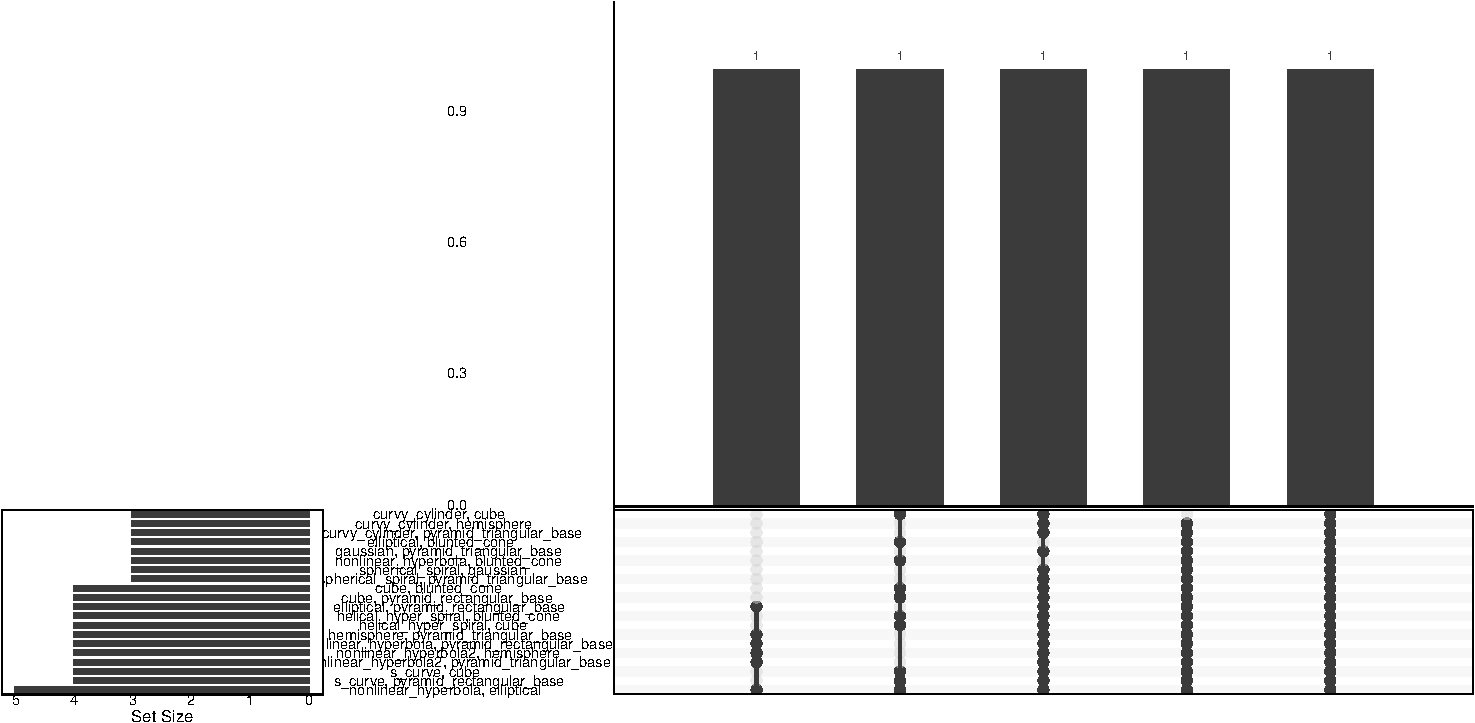
\includegraphics[width=1\linewidth,height=\textheight,keepaspectratio]{chapters/05-chap5_files/figure-pdf/fig-upset-two-1.pdf}

}

\caption{\label{fig-upset-two}UpSet plot showing intersections of
misidentified data structure components across NLDR methods. Each
horizontal bar on the left represents the number of times a particular
data structure component was misidentified. The vertical bars indicate
intersections --- combinations of NLDR methods that share the same
misidentified components. The most frequently co-misidentified
components across methods are nonlinear\_hyperbola + elliptical,
s\_curve + pyramid\_rectangular\_base, s\_curve + cube,
nonlinear\_hyperbola2 + pyramid\_triangular\_base, nonlinear\_hyperbola2
+ hemisphere, nonlinear\_hyperbola + pyramid\_rectangular\_base,
hemisphere + pyramid\_triangular\_base, helical\_hyper\_spiral + cube,
helical\_hyper\_spiral + blunted\_cone, elliptical +
pyramid\_rectangular\_base, cube + pyramid\_rectangular\_base, cube +
blunted\_cone, spherical\_spiral + pyramid\_triangular\_base,
spherical\_spiral + gaussian, nonlinear\_hyperbola + blunted\_cone,
gaussian + pyramid\_triangular\_base, elliptical + blunted\_cone,
curvy\_cylinder + pyramid\_triangular\_base, curvy\_cylinder +
hemisphere, and, curvy\_cylinder + cube, suggesting these structures are
more challenging for multiple NLDR techniques to preserve accurately.}

\end{figure}%

\begin{table}
\centering
\resizebox{\ifdim\width>\linewidth\linewidth\else\width\fi}{!}{
\begin{tabular}{llr}
\toprule
component & methods & num\_methods\\
\midrule
conic\_spiral, filled\_hexagonal\_pyramid & PaCMAP, PHATE , tSNE & 3\\
conic\_spiral, gaussian & PaCMAP, PHATE , tSNE & 3\\
conic\_spiral, pyramid\_triangular\_base & PaCMAP, PHATE , tSNE  , UMAP & 4\\
crescent, cube & PaCMAP, PHATE , tSNE  , UMAP & 4\\
crescent, filled\_hexagonal\_pyramid & PaCMAP, PHATE , UMAP & 3\\
crescent, hemisphere & PaCMAP, PHATE , UMAP & 3\\
crescent, pyramid\_rectangular\_base & PaCMAP, PHATE , tSNE & 3\\
cube, blunted\_cone & PaCMAP, PHATE , tSNE & 3\\
cube, pyramid\_rectangular\_base & PaCMAP, PHATE , TriMAP, tSNE & 4\\
curv, blunted\_cone & PaCMAP, PHATE , tSNE & 3\\
curv, elliptical & PaCMAP, PHATE , tSNE  , UMAP & 4\\
curv, pyramid\_rectangular\_base & PaCMAP, PHATE , tSNE  , UMAP & 4\\
curv2, filled\_hexagonal\_pyramid & PaCMAP, PHATE , TriMAP, tSNE & 4\\
curv2, gaussian & PaCMAP, PHATE , TriMAP, tSNE  , UMAP & 5\\
curv2, pyramid\_triangular\_base & PaCMAP, PHATE , TriMAP, tSNE & 4\\
curvy\_cylinder, blunted\_cone & PaCMAP, tSNE & 2\\
curvy\_cylinder, cube & PaCMAP, tSNE & 2\\
curvy\_cylinder, hemisphere & PaCMAP, PHATE , TriMAP, tSNE & 4\\
curvy\_cylinder, pyramid\_triangular\_base & PaCMAP, PHATE , TriMAP, tSNE & 4\\
elliptical, blunted\_cone & PaCMAP, PHATE , tSNE  , UMAP & 4\\
elliptical, pyramid\_rectangular\_base & PaCMAP, PHATE , tSNE  , UMAP & 4\\
gaussian, filled\_hexagonal\_pyramid & PaCMAP, PHATE , tSNE & 3\\
gaussian, pyramid\_triangular\_base & PaCMAP, PHATE , tSNE & 3\\
helical\_hyper\_spiral, blunted\_cone & PHATE, tSNE & 2\\
helical\_hyper\_spiral, cube & PHATE, tSNE & 2\\
hemisphere, filled\_hexagonal\_pyramid & PHATE, tSNE & 2\\
hemisphere, pyramid\_triangular\_base & PHATE, tSNE & 2\\
nonlinear\_hyperbola, blunted\_cone & PHATE, tSNE & 2\\
nonlinear\_hyperbola2, pyramid\_triangular\_base & PHATE, tSNE & 2\\
s\_curve, cube & PHATE, tSNE & 2\\
s\_curve, filled\_hexagonal\_pyramid & PHATE, tSNE & 2\\
s\_curve, hemisphere & PHATE, tSNE , UMAP & 3\\
s\_curve, pyramid\_rectangular\_base & PHATE, tSNE & 2\\
spherical\_spiral, gaussian & PHATE, tSNE & 2\\
spherical\_spiral, pyramid\_triangular\_base & PHATE, tSNE , UMAP & 3\\
nonlinear\_hyperbola2, blunted\_cone & PHATE, tSNE & 2\\
nonlinear\_hyperbola2, cube & PHATE, tSNE & 2\\
\bottomrule
\end{tabular}}
\end{table}

\subsubsection{Three component}\label{three-component}

The third UpSet plot (Figure~\ref{fig-upset-three}) highlights cases
where misidentifications occurred due to complex interactions among
three components within a dataset. These represent the most difficult
configurations, where multiple structural and density variations
coexist.

Frequent co-misidentified triplets included s\_curve + cube +
pyramid\_rectangular\_base, nonlinear\_hyperbola2 + hemisphere +
pyramid\_triangular\_base, nonlinear\_hyperbola + elliptical +
pyramid\_rectangular\_base, helical\_hyper\_spiral + cube +
blunted\_cone, spherical\_spiral + gaussian + pyramid\_triangular\_base,
nonlinear\_hyperbola + elliptical + blunted\_cone, curvy\_cylinder +
hemisphere + pyramid\_triangular\_base, curvy\_cylinder + cube +
blunted\_cone, and crescent + cube + pyramid\_rectangular\_base.

Most of these triplets involve at least one curved or spiral component
combined with a polyhedral structure, which appears to amplify
projection distortion. PHATE and tSNE were again the dominant
contributors, followed by PaCMAP, while TriMAP rarely misidentified
three-component mixtures. The frequent co-occurrence of such errors
suggests that preserving relative scaling among non-linear surfaces and
multi-faceted shapes remains a key limitation of locally focused NLDR
methods.

\begin{figure}

\centering{

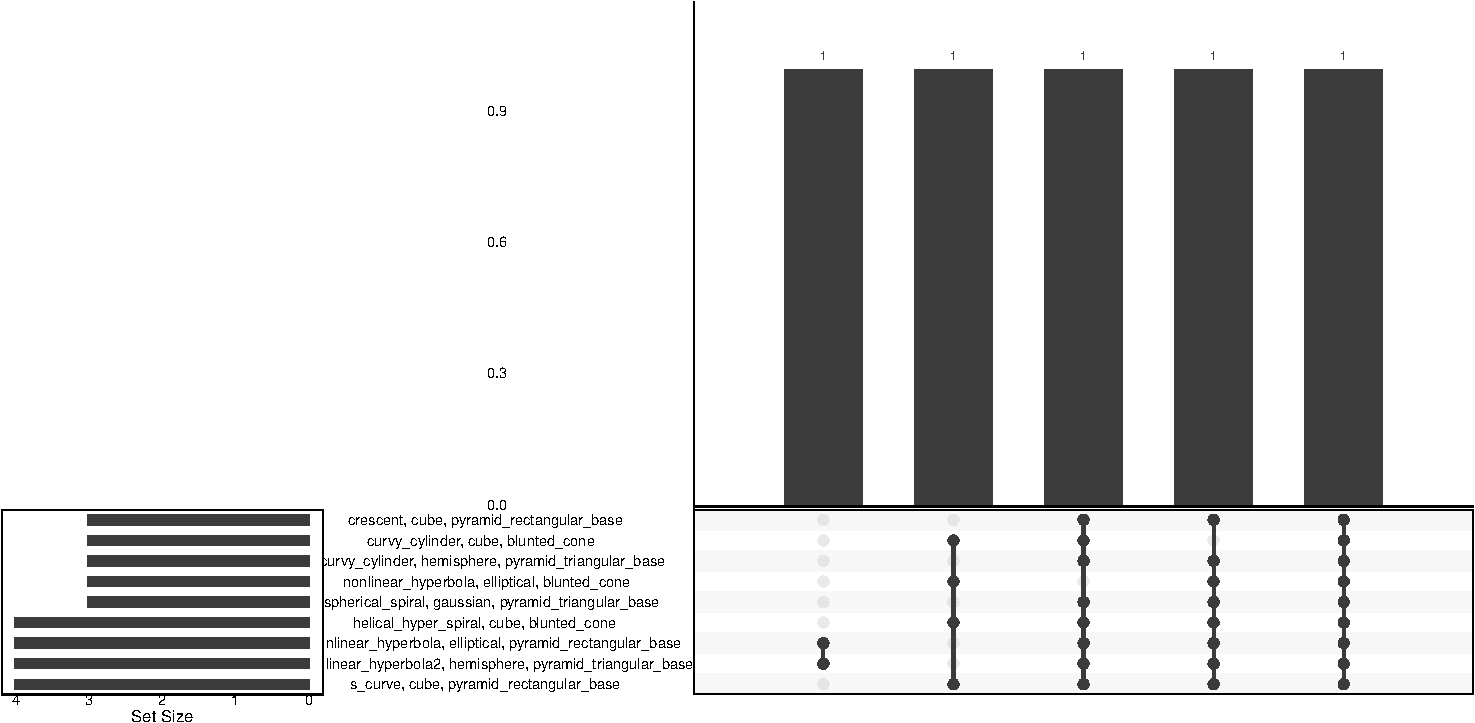
\includegraphics[width=1\linewidth,height=\textheight,keepaspectratio]{chapters/05-chap5_files/figure-pdf/fig-upset-three-1.pdf}

}

\caption{\label{fig-upset-three}UpSet plot showing intersections of
misidentified data structure components across NLDR methods. Each
horizontal bar on the left represents the number of times a particular
data structure component was misidentified. The vertical bars indicate
intersections --- combinations of NLDR methods that share the same
misidentified components. The most frequently co-misidentified
components across methods are s\_curve + cube +
pyramid\_rectangular\_base, nonlinear\_hyperbola2 + hemisphere +
pyramid\_triangular\_base, nonlinear\_hyperbola + elliptical +
pyramid\_rectangular\_base, helical\_hyper\_spiral + cube +
blunted\_cone, spherical\_spiral + gaussian + pyramid\_triangular\_base,
nonlinear\_hyperbola + elliptical + blunted\_cone, curvy\_cylinder +
hemisphere + pyramid\_triangular\_base, curvy\_cylinder + cube +
blunted\_cone, crescent + cube + pyramid\_rectangular\_base, suggesting
these structures are more challenging for multiple NLDR techniques to
preserve accurately.}

\end{figure}%

\begin{table}
\centering
\resizebox{\ifdim\width>\linewidth\linewidth\else\width\fi}{!}{
\begin{tabular}{llr}
\toprule
component & methods & num\_methods\\
\midrule
conic\_spiral, gaussian, filled\_hexagonal\_pyramid & PaCMAP, PHATE , tSNE & 3\\
conic\_spiral, gaussian, pyramid\_triangular\_base & PaCMAP, PHATE , UMAP & 3\\
crescent, cube, pyramid\_rectangular\_base & PaCMAP, PHATE , tSNE & 3\\
crescent, hemisphere, filled\_hexagonal\_pyramid & PaCMAP, PHATE , tSNE  , UMAP & 4\\
curv, elliptical, blunted\_cone & PaCMAP, PHATE , TriMAP, tSNE & 4\\
curv, elliptical, pyramid\_rectangular\_base & PaCMAP, tSNE & 2\\
curv2, gaussian, filled\_hexagonal\_pyramid & PaCMAP, PHATE , TriMAP, tSNE & 4\\
curv2, gaussian, pyramid\_triangular\_base & PaCMAP, PHATE , tSNE  , UMAP & 4\\
curvy\_cylinder, cube, blunted\_cone & PaCMAP, PHATE , tSNE & 3\\
curvy\_cylinder, hemisphere, pyramid\_triangular\_base & PHATE, tSNE & 2\\
helical\_hyper\_spiral, cube, blunted\_cone & PHATE, tSNE & 2\\
nonlinear\_hyperbola, elliptical, blunted\_cone & PHATE, tSNE & 2\\
s\_curve, cube, pyramid\_rectangular\_base & PHATE, tSNE & 2\\
s\_curve, hemisphere, filled\_hexagonal\_pyramid & PHATE, tSNE & 2\\
spherical\_spiral, gaussian, pyramid\_triangular\_base & PHATE, tSNE , UMAP & 3\\
nonlinear\_hyperbola2, cube, blunted\_cone & PHATE, tSNE & 2\\
\bottomrule
\end{tabular}}
\end{table}

\section{Limitations}\label{sec-limitations}

One of the main drawbacks of visual experiments is their reliance on
human judgments. In this context, the effectiveness of identifying the
\gD{} NLDR plot and the tour from the same data can be dependent on the
perceptual ability and visual skills of the individual. However, when
the results from multiple individuals are combined, the overall quality
and robustness of the outcome is considerably high.

It is important to remove HTML widget elements such as controls,
interactivity, and \gD{} plot elements such as axis labels and text that
might introduce bias. We recommend using a crowd-sourcing service like
Prolific (\citeproc{ref-palan2018}{\textbf{palan2018?}}) to access
high-quality data, as it is a time- and cost-effective way.

In this study, we used a specific data structure consisting of three
distinct clusters, each with unique shapes. Two of the clusters are in
close proximity to one another, while the third cluster is located
farther away. Each cluster varies in the number of points it contains.
We selected this data structure because it is simple.

To keep the experiment fair and consistent across trials, we
approximately fixed the distance between the clusters in each data
structure. We also used five distance scale factors to gradually change
how far apart the clusters were. While this controlled setup makes it
easier to interpret the results, it does limit how well the findings
apply to more complex data structures with uneven or irregular cluster
arrangements.

\section{Conclusions}\label{sec-conclusion}

This study provides empirical evidence that NLDR methods differ
substantially in how well they preserve high-dimensional structures that
are perceptually meaningful for classification and clustering. By
combining a controlled simulation of three clusters with varying
separation, shape, and size, and a human recognition experiment, we
quantified how structural separability in the original space translates
into correct identification of clusters in \gD{} representations.

Our results reveal consistent differences among NLDR methods. UMAP and
PaCMAP produced layouts where greater high-dimensional
separation---quantified by both the scaled BW ratio and the exponential
of the scaled minimum inter-cluster distance---led to higher
probabilities of correct identification. These methods explicitly
optimize for both local and global relationships: UMAP through fuzzy
topological preservation and PaCMAP through adaptive pairwise
constraints that balance local and mid-range distances. This dual
emphasis likely explains their superior perceptual alignment with the
true \pD{} structure. TriMAP showed a similar but less pronounced trend,
consistent with its triplet-based loss that prioritizes preservation of
global relationships.

In contrast, tSNE exhibited a negative association between separability
and correct identification, consistent with prior findings that its
Kullback--Leibler divergence loss exaggerates local density differences
at the expense of global geometry. As clusters became more distinct in
the high-dimensional space, tSNE's optimization fragmented global
relationships, yielding visually appealing but structurally misleading
layouts. PHATE, which emphasizes manifold continuity rather than
discrete grouping through potential distances, showed no systematic
relationship between separability and accuracy, aligning with its design
focus on smooth transitions rather than cluster fidelity.

Visual inspection of misidentifications further supports these
quantitative results. Curvilinear or non-linear manifolds---such as
\emph{s\_curve}, \emph{helical\_hyper\_spiral}, and
\emph{nonlinear\_hyperbola}---were most often misrepresented,
particularly when paired with compact clusters like \emph{cube} or
\emph{blunted\_cone}. Methods emphasizing local continuity, such as tSNE
and PHATE, tended to merge or over-separate these curved structures,
while PaCMAP and UMAP occasionally distorted their global positioning
when cluster density or scale varied. TriMAP, though better at
maintaining overall spatial relationships, frequently compressed curved
manifolds against more compact forms, leading to overlap or shape loss.
These systematic misidentifications underscore how each method's
underlying loss function---balancing local versus global
preservation---directly shapes perceptual fidelity in the resulting
embeddings.

Overall, these findings emphasize that NLDR methods should be evaluated
not only by visual appearance but by their alignment between
quantitative structure and perceptual interpretation. Methods like UMAP
and PaCMAP appear to maintain interpretable geometric fidelity across
varying levels of separation, while tSNE and PHATE prioritize
alternative aspects of structure. The implication for statistical
graphics is that perceptually faithful embeddings are not guaranteed by
standard algorithmic performance metrics alone.

Future work should extend these analyses to a wider range of
experimental conditions, including different noise levels, sample sizes,
and dimensionalities, to test the robustness of perceptual fidelity
across contexts. Comparing with linear methods such as PCA or supervised
embeddings could also clarify whether the observed effects are unique to
non-linear transformations or reflect broader perceptual tendencies in
cluster interpretation. In addition, exploring alternative data
structures---such as overlapping clusters, hierarchical manifolds, or
continuous gradients---would help determine how general these perceptual
biases are across more complex topologies. Integrating automated visual
diagnostics, for example using computer-vision or deep-learning--based
similarity metrics, could complement human judgment and provide
objective measures of structure preservation. Finally, combining
interactive visualization environments with eye-tracking or
cognitive-load assessments could reveal how users process and trust NLDR
layouts in real time. Such advances would not only improve the
interpretability of dimensionality reduction methods but also support
the development of human-centered evaluation frameworks that bridge
statistical validity and perceptual understanding in high-dimensional
data visualization.

\section{Acknowledgments}\label{acknowledgments-1}

A pilot study was conducted with sample subjects from the working group
of the Department of Econometrics and Business Statistics, Monash
University. This pilot study allowed us to estimate the study's
completion time and the effect size and fine-tune the application.

These R packages were used for the work: \texttt{tidyverse} (Wickham et
al. (\citeproc{ref-hadley2019}{2019})), \texttt{lme4}
((\citeproc{ref-douglas2015}{\textbf{douglas2015?}})),
\texttt{broom.mixed} ((\citeproc{ref-ben2024}{\textbf{ben2024?}})),
\texttt{ggbeeswarm} ((\citeproc{ref-erik2023}{\textbf{erik2023?}})),
\texttt{emmeans} ((\citeproc{ref-russell2025}{\textbf{russell2025?}})),
\texttt{patchwork} (Pedersen (\citeproc{ref-thomas2024}{2024})),
\texttt{colorspace} (Zeileis et al. (\citeproc{ref-achim2020}{2020})),
\texttt{kableExtra} (Zhu (\citeproc{ref-hao2024}{2024})),
\texttt{conflicted} (Wickham (\citeproc{ref-hadley2023}{2023})),
\texttt{UpSetR} ((\citeproc{ref-nils2019}{\textbf{nils2019?}})),
\texttt{Rtsne} (Krijthe (\citeproc{ref-jesse2015}{2015})), \texttt{umap}
(Konopka (\citeproc{ref-tomasz2023}{2023})), \texttt{phateR}(Moon et al.
(\citeproc{ref-moon2019}{2019})), \texttt{reticulate} (Ushey et al.
(\citeproc{ref-kevin2024}{2024})), \texttt{langevitour} (Harrison
(\citeproc{ref-harisson2024}{2023})), \texttt{gridExtra}
((\citeproc{ref-baptiste2017}{\textbf{baptiste2017?}})), \texttt{shiny}
((\citeproc{ref-winston2024}{\textbf{winston2024?}})),
\texttt{shinydashboard}
((\citeproc{ref-winston2025}{\textbf{winston2025?}})),
\texttt{shinythemes}
((\citeproc{ref-winston2021}{\textbf{winston2021?}})), \texttt{bslib}
((\citeproc{ref-carson2025}{\textbf{carson2025?}})), \texttt{shinyjs}
((\citeproc{ref-dean2021}{\textbf{dean2021?}})), \texttt{DT}
((\citeproc{ref-yihui2016}{\textbf{yihui2016?}})), \texttt{googledrive}
((\citeproc{ref-lucy2025}{\textbf{lucy2025?}})), \texttt{googleAuthR}
((\citeproc{ref-mark2024}{\textbf{mark2024?}})), \texttt{googlesheets4}
((\citeproc{ref-jennifer2025}{\textbf{jennifer2025?}})),
\texttt{shinyalert} ((\citeproc{ref-dean2024a}{\textbf{dean2024a?}})),
\texttt{shinypop} ((\citeproc{ref-fanny2024}{\textbf{fanny2024?}})),
\texttt{randomNames}
((\citeproc{ref-damian2024}{\textbf{damian2024?}})),
\texttt{shinyfullscreen}
((\citeproc{ref-etienne2021}{\textbf{etienne2021?}})),
\texttt{shinyWidgets}
((\citeproc{ref-victor2025}{\textbf{victor2025?}})), \texttt{hms}
((\citeproc{ref-kirill2025}{\textbf{kirill2025?}})),
\texttt{shinythemes}
((\citeproc{ref-winston2021}{\textbf{winston2021?}})), and
\texttt{shinycssloaders}
((\citeproc{ref-dean2024b}{\textbf{dean2024b?}})). These \texttt{python}
packages were used for the work: \texttt{trimap} (Amid and Warmuth
(\citeproc{ref-amid2022}{2022})) and \texttt{pacmap} (Wang et al.
(\citeproc{ref-yingfan2021}{2021})).

\section{Supplementary Materials}\label{supplementary-materials}

All the materials to reproduce the paper can be found at
\url{https://github.com/JayaniLakshika/paper-vis-experiment}.

Appendix: The appendix includes more details about the data structures
and their tSNE, UMAP, PHATE, PaCMAP, and TriMAP layouts used in the
study (appendix.pdf, Portable Document Format file).

XXX Add Match-a-roo experiment links

\bookmarksetup{startatroot}

\chapter{Development of an interactive and dynamic graphics system for
NLDR users}\label{sec-fifth-paper}

\section{Introduction}\label{introduction-4}

Non-linear dimensionality reduction (NLDR) methods such as tSNE (Maaten
and Hinton (\citeproc{ref-laurens2008}{2008})) and UMAP (McInnes et al.
(\citeproc{ref-leland2018}{2018})) have become essential tools for
exploring and visualizing high-dimensional data across diverse
scientific disciplines. These techniques enable researchers to uncover
structures, clusters, and patterns that are not immediately visible in
the original feature space. However, the flexibility and power of these
methods come with challenges: the quality and interpretability of
low-dimensional embeddings are often highly sensitive to hyper-parameter
choices, random initialization, and characteristics of the underlying
data. As a result, identifying the most meaningful and faithful
representation typically requires iterative experimentation, systematic
evaluation, and domain expertise.

To address these challenges, we introduce \texttt{menuraR}
(\emph{monitoring embeddings of nonlinear unfoldings for representation
and analysis in R}), an interactive Shiny application created to
facilitate the evaluation of NLDR layouts. Building on the functionality
of the \texttt{quollr} R package
((\citeproc{ref-jayani2025}{\textbf{jayani2025?}})), \texttt{menuraR}
provides a graphical user interface that enables users to compare
multiple NLDR layouts, explore the effects of different hyper-parameter
settings, and apply diagnostic tools for evaluating NLDR layout(s).

These capabilities are delivered through an intuitive interface that
eliminates the need for programming, thereby lowering the technical
barrier for applied researchers, students, and methodologists.

A key advantage of \texttt{menuraR} is its accessibility. The
application is fully web-based, requiring no local installation of R or
package management. Centralized hosting ensures that users always access
the most up-to-date version, while reproducibility is supported through
logging and open availability of the underlying code. In this way,
\texttt{menuraR} enhances transparency in NLDR evaluation and fosters
broader adoption of rigorous visualization practices.

This paper introduces version \(0.1.0\) of \texttt{menuraR}, outlining
its implementation, core features, and intended use cases. We
demonstrate how the application can inform NLDR choices, highlight key
visual diagnostics, and support both exploratory data analysis and
teaching.

\section{Implementation}\label{implementation-2}

The \texttt{menuraR} application is implemented in the R programming
language using the \texttt{shiny} package
((\citeproc{ref-winston2025a}{\textbf{winston2025a?}})), which provides
the reactive programming framework needed for building interactive web
applications. The front end integrates functionality from
\texttt{htmltools} ((\citeproc{ref-joe2024}{\textbf{joe2024?}})) to
dynamically render markdown documentation within the application,
ensuring that explanatory material and usage guidance are seamlessly
incorporated alongside interactive elements. To enhance usability, the
application employs \texttt{shinycssloaders}
((\citeproc{ref-dean2024}{\textbf{dean2024?}})), which provides
responsive loading animations during long-running computations.

From an architectural perspective, \texttt{menuraR} is structured around
a separation between the user interface (UI) and the computational back
end. The UI components: buttons, menus, and plotting panels are rendered
through Shiny's reactive layer, which updates outputs in real time in
response to user interactions. Computational tasks, such as fitting tSNE
(\citeproc{ref-jesse2015}{Krijthe 2015}) or UMAP
(\citeproc{ref-james2025}{\textbf{james2025?}}) embeddings, are
delegated to the R back end and are executed primarily through functions
provided by the \texttt{quollr} package
((\citeproc{ref-jayani2025}{\textbf{jayani2025?}})). This modular design
ensures that new dimensionality reduction methods or diagnostics can be
incorporated with minimal changes to the user-facing interface.

For deployment, \texttt{menuraR} is hosted on the
\href{https://shinyapps.io}{shinyapps.io} platform, a managed,
cloud-based service that supports full R integration. This allows users
to run the application directly from any modern web browser without the
need to install additional software or manage dependencies locally. The
hosted version currently supports the generation of NLDR layouts using
tSNE and UMAP, leveraging implementations in the R ecosystem.

This design supports accessibility, reproducibility, and extensibility.
Accessibility is achieved through a web-based interface that eliminates
the need for local installation. Reproducibility is ensured by
maintaining a consistent server-side computational environment across
sessions. Extensibility follows from the modular linkage between the
Shiny interface and the \texttt{quollr} computational back end, which
fits model(s) for the NLDR layout(s), computes RWBSS for different
binwidths, visualizes the model and generates diagnostics without
altering the core interface.

\section{The Shiny application}\label{the-shiny-application}

The \texttt{menuraR} app contains four main three tabs: (1) Data Upload,
(2) Compare NLDR Layouts, and (3) Model diagnostics. Each tab includes
numbered steps and clear instructions, guiding users from data input to
interpretation of results.

\subsection{Data upload}\label{data-upload}

Analysis in \texttt{menuraR} begins in two ways: by uploading
user-provided high-dimensional data or by using one of the built-in
example datasets. Two datasets are provided within the application:
C-shaped Clusters, a synthetic dataset illustrating nonlinear structure,
and PBMC, a biological single-cell dataset for real-world exploration
(\citeproc{ref-rahul2025}{\textbf{rahul2025?}}). If the user uploads own
high-dimensional data, the file should be a CSV and the CSV must have a
unique ID column, with data columns prefixed by the letter ``x'' (e.g.,
\texttt{x1}, \texttt{x2}, etc.).

Once the high-dimensional data uploaded, under ``choose your data
source'', users can specify their data source: ``Upload your own data'',
or ``Generate default tSNE and UMAP layouts''. Selecting \emph{Upload
your own NLDR data} activates the uploaded NLDR layouts and metadata for
comparison. The NLDR file is a CSV file of pre-computed NLDR, which
contains embedding data must be labeled as \texttt{emb1} and
\texttt{emb2}, and each layout should have its columns named with a
prefix corresponding to the layout number, such as \texttt{1\_emb1} and
\texttt{1\_emb2} for the first layout. Also, the meta data CSV file
includes the NLDR layout name (e.g., 1, 2, etc.), the method used (like
UMAP or tSNE), and any hyper-parameters formatted with the parameter
name followed by its value, separated by a dash (e.g., perplexity-30 for
tSNE). All uploaded files must be under \(100\) MB in size, and it is
essential that each dataset follows the variable naming conventions
required by the web application. Alternatively, users may choose
\emph{Generate default tSNE and UMAP layouts}, in which case the
application automatically computes two embeddings using default
hyper-parameter settings for tSNE and UMAP.

Once loaded, all available NLDR layouts appear in the ``Your Loaded NLDR
Layouts'' box. Users can select or deselect specific layouts to include
in the comparison.

\subsubsection{Adding additional
layouts}\label{adding-additional-layouts}

The application also allows users to generate additional layouts
directly within the interface. Users select the NLDR method (tSNE or
UMAP), specify hyper-parameters, and click ``Show Layout'' to generate
the embedding. If satisfied, they can add it to the comparison using
``Add Layout''; otherwise, they may adjust the parameters and regenerate
the layout. Multiple additional layouts can be created and compared in
this manner.

Once the desired layouts are finalized, users click ``Start Analysis''
to proceed automatically to the next tab, Compare NLDR Layouts, where
the evaluation and comparison of embeddings take place.

\begin{center}
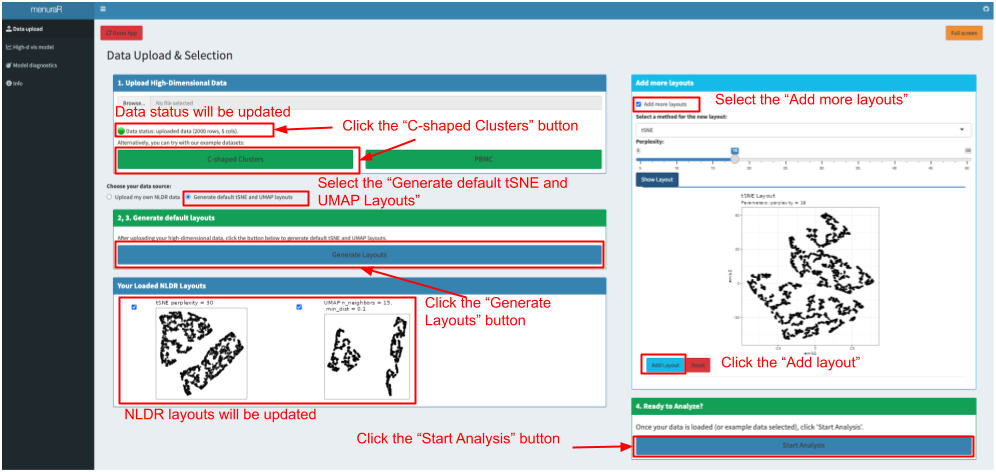
\includegraphics[width=1\linewidth,height=\textheight,keepaspectratio]{chapters/../figures/menuraR/menuraR_ui1.png}
\end{center}

\subsection{Compare NLDR Layouts}\label{compare-nldr-layouts}

Users can view the \(2\text{-}D\) NLDR layouts that have been selected
to compare. The app also generates a plot showing the Root Within Bin
Sum of Square (RWBSS) against the bandwidth parameter (\(a_1\)) and
identifies the ``best'' representation that yields the lowest RWBSS for
that specific \(a_1\). Users can modify the \(a_1\) value to see what
layout performs best for the chosen bandwidth.

Furthermore, users have the option to download the \(2\text{-}D\)
layouts, corresponding data, the RWBSS versus bin width plot, and the
summary table, which contains error, RWBSS, the number of bins along the
x-axis (\(b1\)), the number of bins along the y-axis (\(b2\)), the total
number of bins (\(b\)), the number of non-empty bins (\(m\)), the bin
width (\(a_1\)), the bin height (\(a_2\)), standardized bin counts
(\(w_h\)), and NLDR method id.

\begin{center}
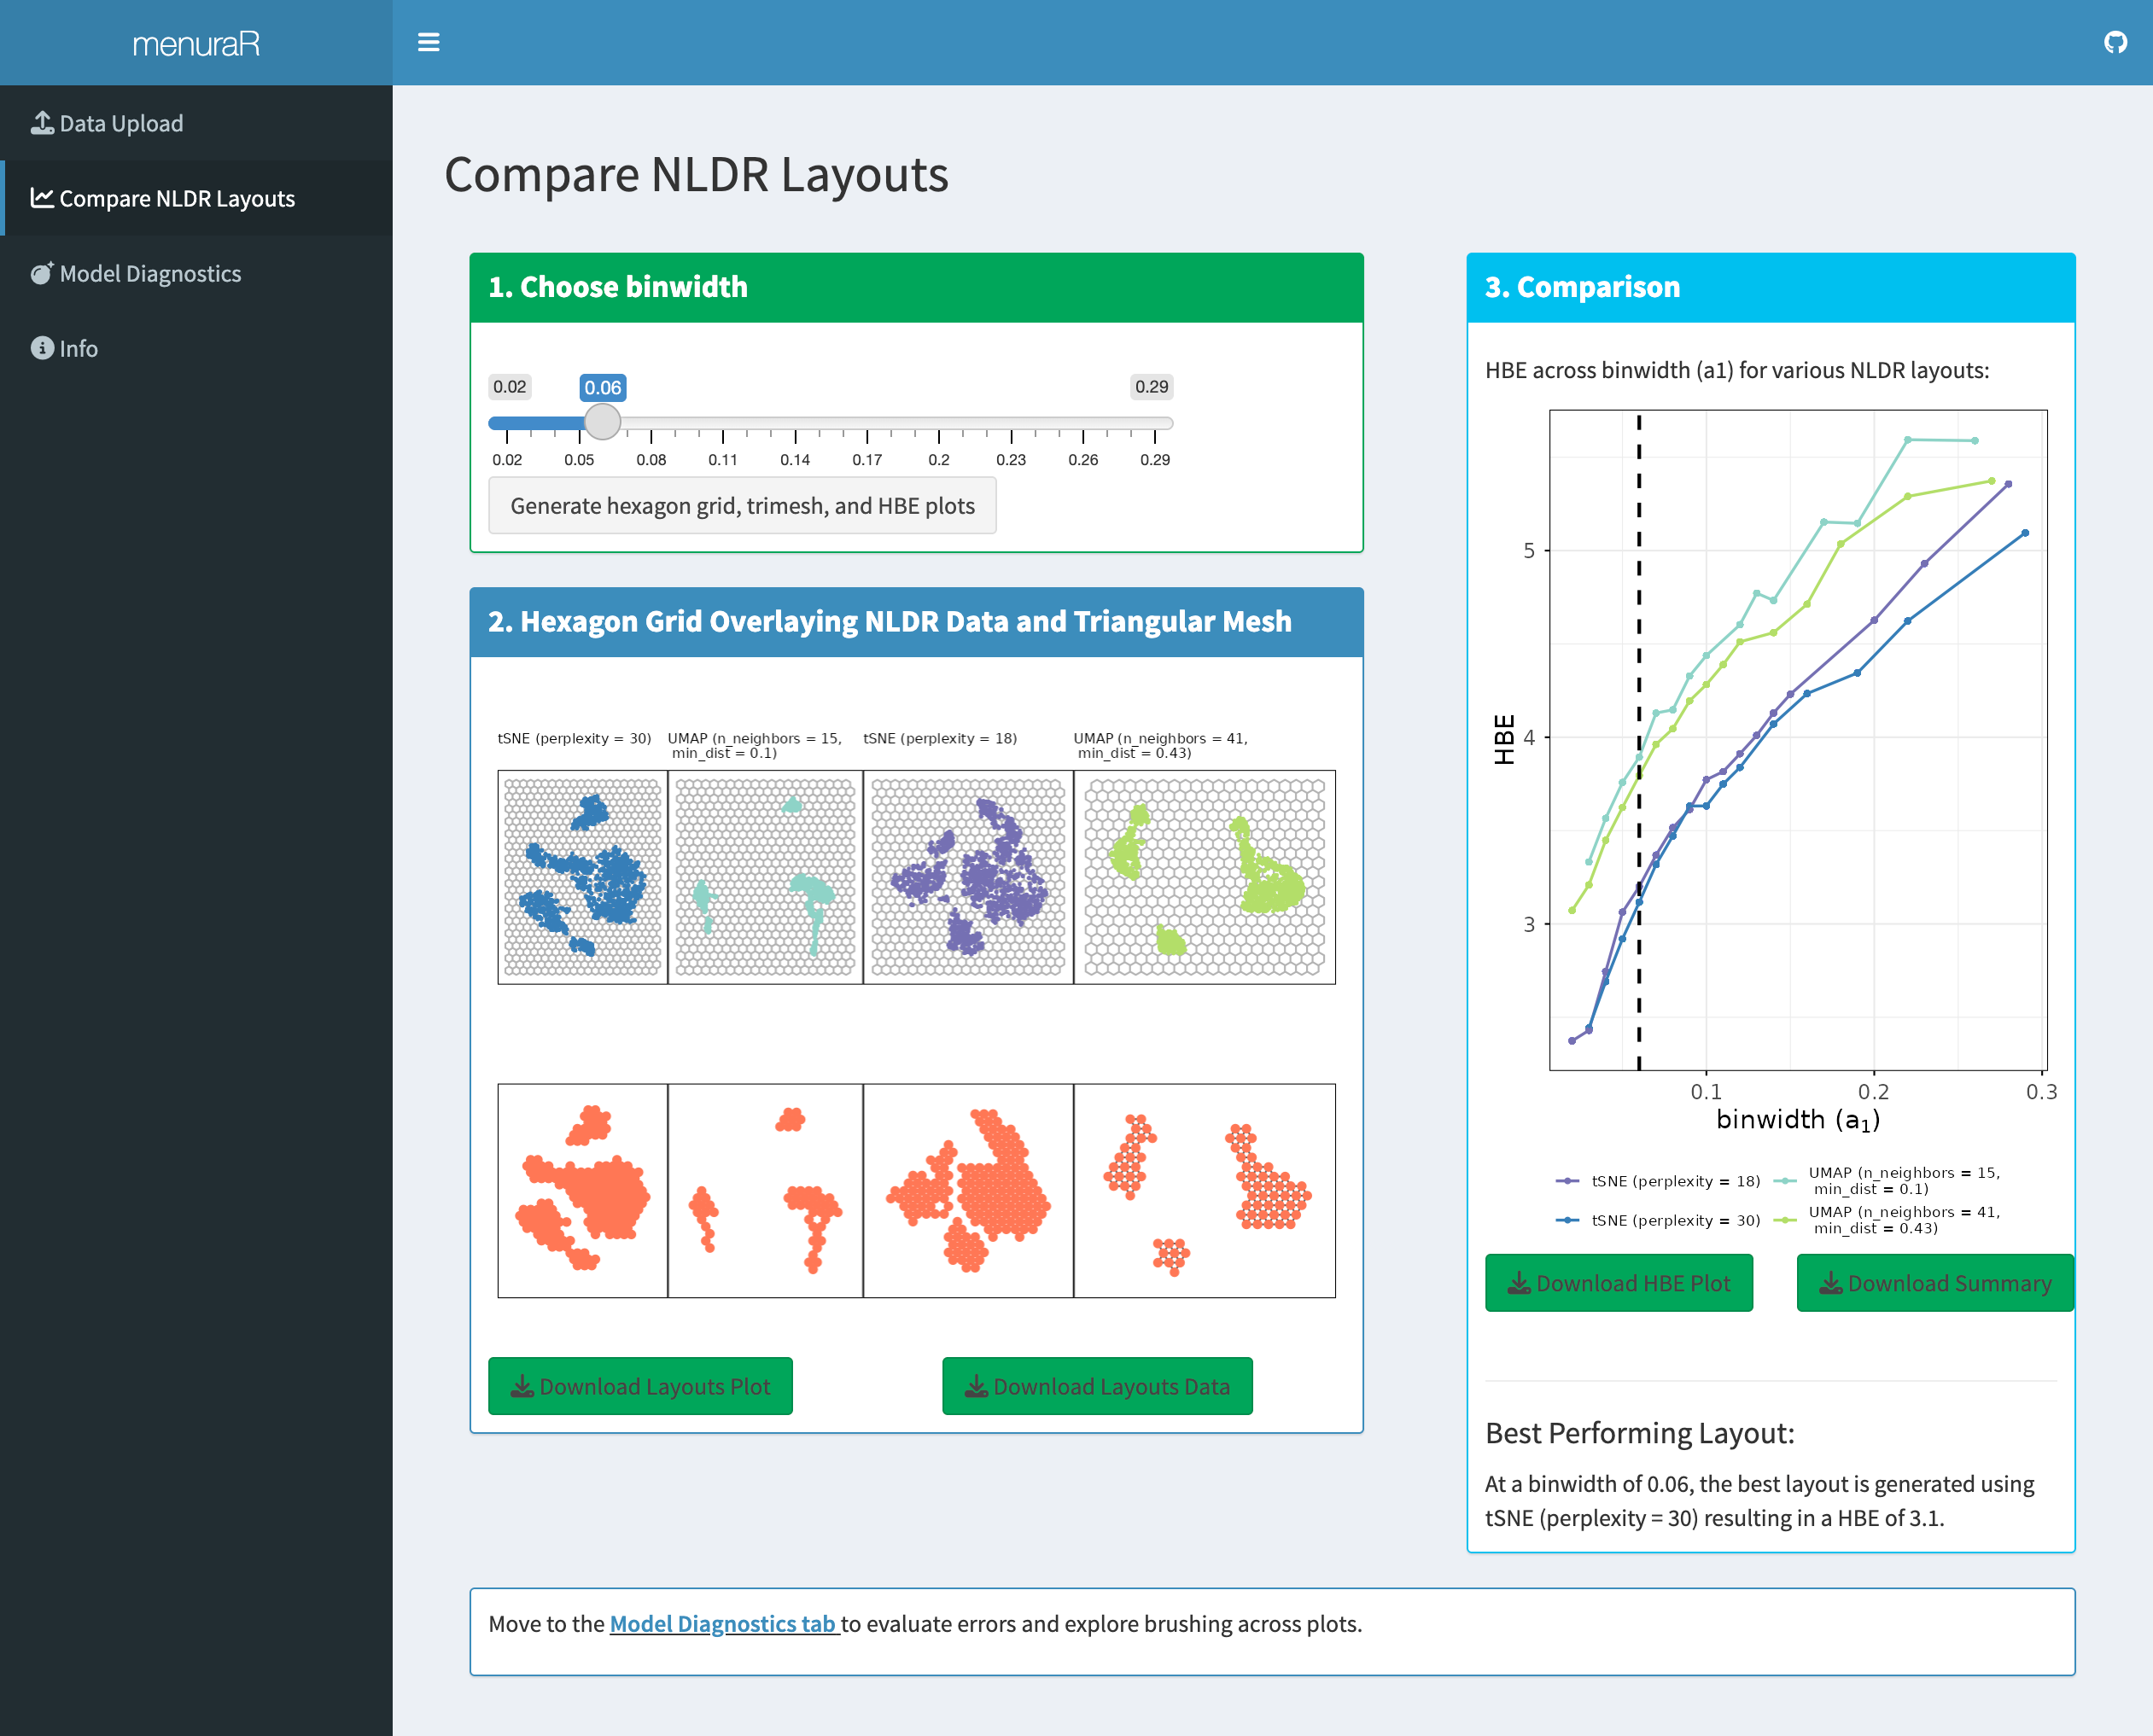
\includegraphics[width=1\linewidth,height=\textheight,keepaspectratio]{chapters/../figures/menuraR/menuraR_ui2.png}
\end{center}

\subsection{Model diagnostics}\label{model-diagnostics}

Once the best representation is selected, interactive plots are
generated to display the high-dimensional model error, the best
\(2\text{-}D\) layout, and a tour view of the model overlaying the
high-dimensional data. This interactivity allows users to identify where
the model fits well, where it better in some subspaces, and where it
fails to match the data. Additionally, users can explore the mapping
between the \(2\text{-}D\) layout and the high-dimensional data.
Importantly, model diagnostics are not limited to the best NLDR layout;
other layouts can also be selected and examined for comparison.

\begin{center}
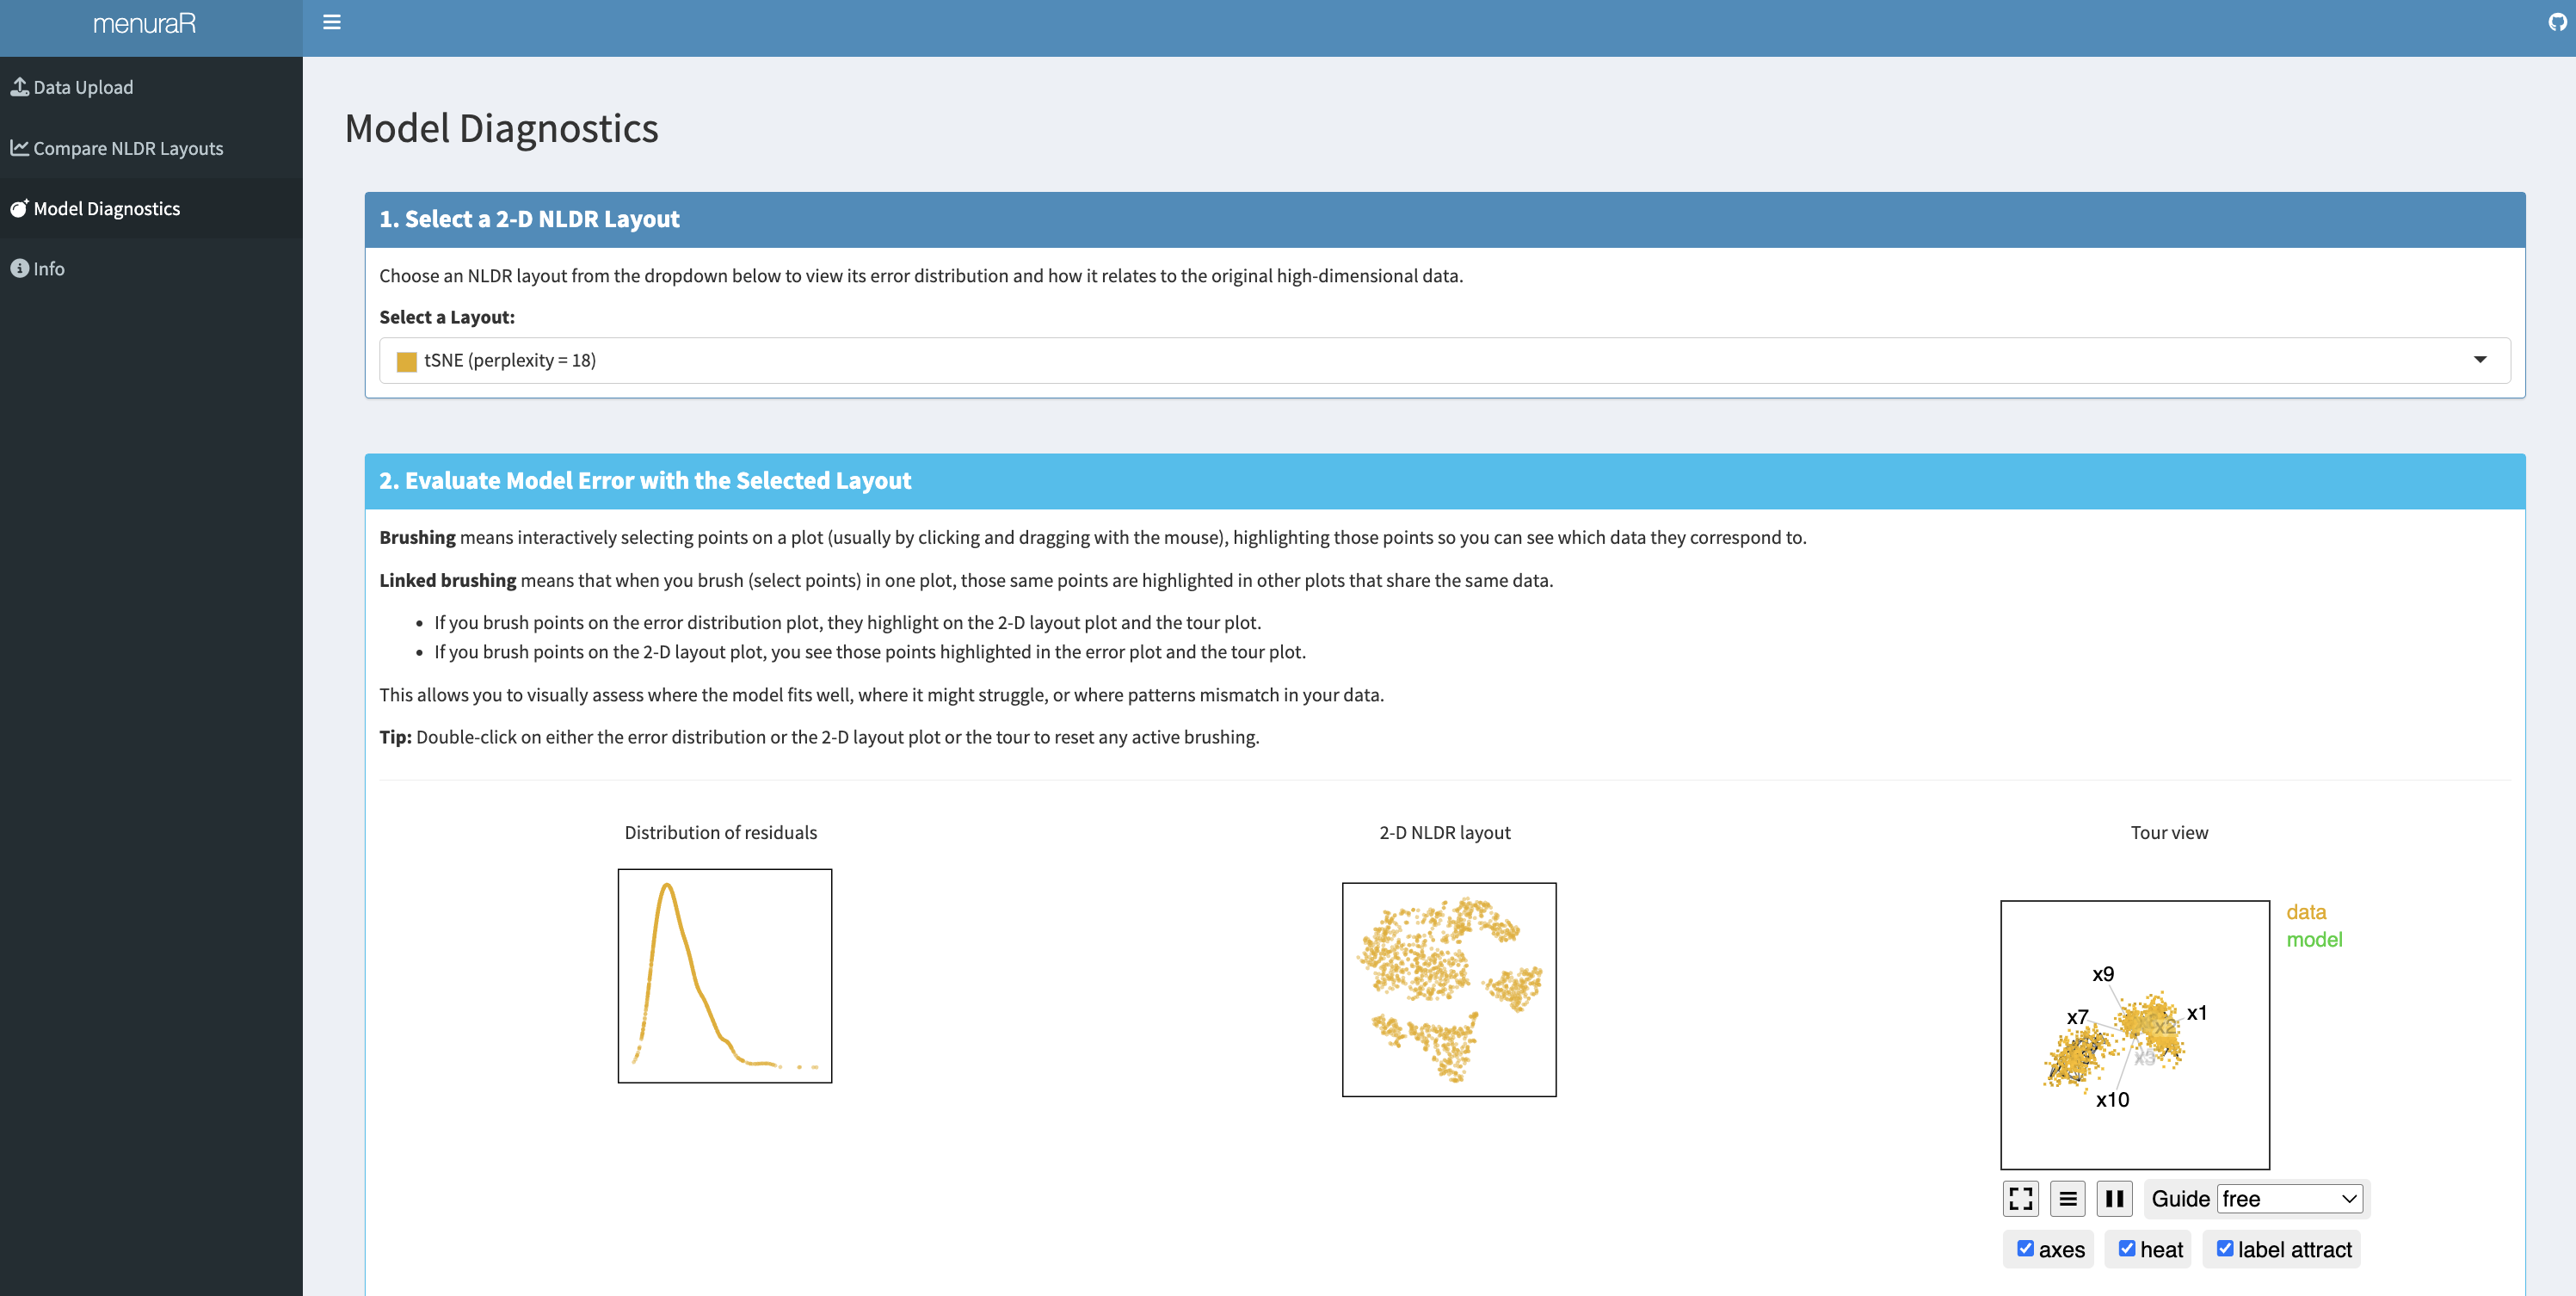
\includegraphics[width=1\linewidth,height=\textheight,keepaspectratio]{chapters/../figures/menuraR/menuraR_ui3.png}
\end{center}

\section{Limitations}\label{limitations}

Currently, \texttt{menuraR} supports two NLDR methods tSNE and UMAP
executed within the R environment on shinyapps.io. Performance may vary
depending on dataset size and browser memory limits, as computations are
handled server-side.

\section{Conclusions}\label{conclusions}

This paper introduces \texttt{menuraR}, a web-based interface designed
to assist in the evaluation and selection of the most reasonable NLDR
layout(s). Although NLDR methods such as tSNE, and, UMAP are widely used
for visualizing high-dimensional data, interpreting and selecting the
most representative layout can be complex. \texttt{menuraR} addresses
this challenge by providing an accessible, intuitive, and interactive
environment that encapsulates the diagnostic features of the
\texttt{quollr} package, making assistant in NLDR selection feasible for
users with varying levels of technical expertise.

Developed using the R Shiny framework, \texttt{menuraR} eliminates many
of the technical barriers traditionally associated with advanced
statistical software. Users do not need to install additional packages
or configure language-specific environments, which is particularly
valuable for interdisciplinary research teams and educational settings.
The platform allows for comparisons of layouts, visual diagnostics, and
selection criteria.

\section{Availability}\label{availability}

The source code for the Shiny application can be found at
\href{https://github.com/JayaniLakshika/menuraR}{\texttt{github.com/JayaniLakshika/menuraR}}.
Users can access the web interface at
\href{https://menurar.netlify.app/}{\texttt{menurar.netlify.app}}.

\section{Supplementary material}\label{supplementary-material}

All the materials to reproduce the paper can be found at
\href{https://github.com/JayaniLakshika/paper-menuraR.git}{\texttt{github.com/JayaniLakshika/paper-menuraR}}.

\bookmarksetup{startatroot}

\chapter{Conclusion and future plans}\label{sec-conclusion}

This thesis presents four key contributions that collectively advance
the understanding and evaluation of NLDR methods. The work improves NLDR
diagnostics, provides insights into human perception of high-dimensional
structures, develops methods for generating clustering data structures,
and implements user-friendly software tools that support exploratory
analysis and visualization.

\section{Contributions}\label{contributions}

The primary contributions of this research are fourfold. First, we
introduce a novel method for visualizing how NLDR warps data, thereby
improving the diagnostics of NLDR techniques. Second, we conduct a human
subject experiment to investigate the perception and misperception of
NLDR representations, providing evidence on how clusters at varying
distances are identified in comparison to high-dimensional tours. Third,
we develop two R packages: \texttt{quollr}, which implements the
proposed diagnostic method, and \texttt{cardinalR}, which generates
high-dimensional data structures with enhanced features such as added
noise dimensions and background noise. Finally, we create a Shiny
application that provides analysts with a user-friendly interface for
obtaining the most accurate NLDR representation.

The software outputs of this research have been made publicly available
to support transparency and reproducibility. The R package
\texttt{quollr} has been on CRAN since March \(2024\) and has received
\(3656\) downloads from the CRAN mirror; its development version is
hosted on GitHub at \url{https://github.com/jayanilakshika/quollr}. The
R package \texttt{cardinalR} has been available on CRAN since April
\(2024\) and has received \(3862\) downloads from the CRAN mirror, with
the latest development version at
\url{https://github.com/jayanilakshika/cardinalR}. A Shiny application
for \texttt{quollr} is accessible via one of the mirror sites at
\url{https://menurar.netlify.app/}, with its source code available at
\url{https://github.com/JayaniLakshika/menuraR}.

\pandocbounded{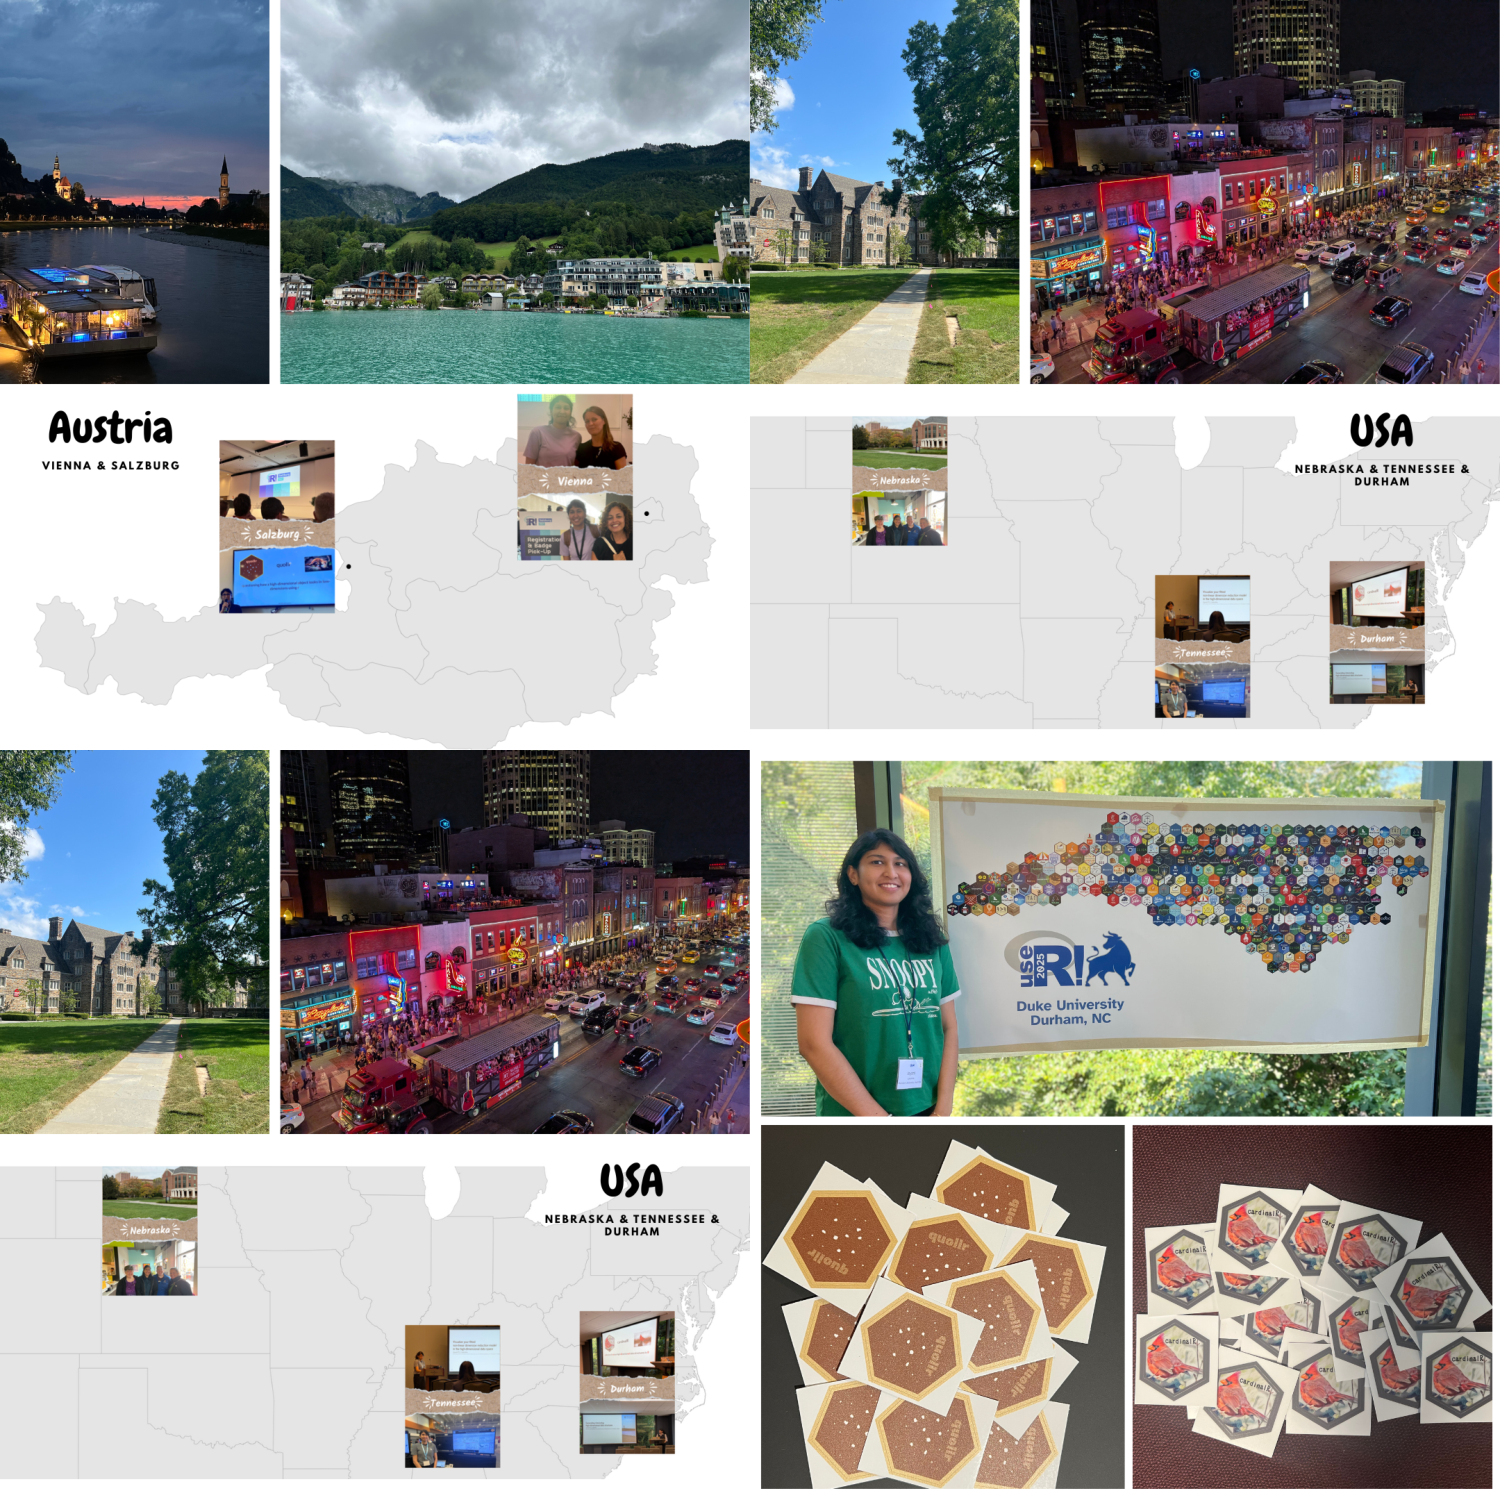
\includegraphics[keepaspectratio]{chapters/07-chap7_files/figure-pdf/unnamed-chunk-1-1.pdf}}

The survey web application, \textbf{Match-a-roo}
(\url{https://ebsmonash.shinyapps.io/Match-a-roo/}), was designed and
implemented in Shiny to collect participant responses and demographic
information. Each subject accessed the survey through the shinyapps.io
server.

All materials associated with this thesis are openly available at
\url{https://github.com/JayaniLakshika/Monash_PhD_thesis}, reflecting
the principles of transparency and reproducible research. The thesis
itself is written in Quarto
(\citeproc{ref-Allaire_Quarto_2024}{\textbf{Allaire\_Quarto\_2024?}})
and published online at
\url{https://jayani-lakshika-phd-thesis.netlify.app}.

In addition, a number of R packages were essential in the development of
this work, including \texttt{tidyverse}
(\citeproc{ref-tidyverse}{\textbf{tidyverse?}}), \texttt{lmtest}
(\citeproc{ref-lmtest}{\textbf{lmtest?}}), \texttt{kableExtra}
(\citeproc{ref-kableextra}{\textbf{kableextra?}}), \texttt{patchwork}
(\citeproc{ref-patchwork}{\textbf{patchwork?}}), \texttt{glue}
(\citeproc{ref-glue}{\textbf{glue?}}), \texttt{ggpcp}
(\citeproc{ref-ggpcp}{\textbf{ggpcp?}}), \texttt{here}
(\citeproc{ref-here}{\textbf{here?}}), and \texttt{knitr}
(\citeproc{ref-knitr}{\textbf{knitr?}}). (Final package list to be
confirmed upon completion of writing.)

\section{Add about polarisR as well.}\label{add-about-polarisr-as-well.}

\section{Future work}\label{future-work}

There are several directions that this work can be developed.

\subsection{\texorpdfstring{Extending our algorithm to NLDR
representations beyond
\(2\text{-}D\)}{Extending our algorithm to NLDR representations beyond 2\textbackslash text\{-\}D}}\label{extending-our-algorithm-to-nldr-representations-beyond-2text-d}

A potential direction for future work is extending the current algorithm
to NLDR results that project into more than two dimensions. While most
existing tools including those developed in this thesis focus on
\(2\text{-}D\) embeddings, exploring projections into higher dimensions
like \(3\text{-}D\) or \(5\text{-}D\) spaces could provide richer
structural information in some settings.

Binning into cubes (\(3\text{-}D\) or higher) could be performed
relatively easily and used as the basis for constructing a wireframe
representation of the fitted model. The algorithm for convex hull
computation in \(p\)-dimensions, as described by Barber et al.
(\citeproc{ref-barber1996}{1996}) and implemented in related software
(Laurent (\citeproc{ref-stephane2023}{2023})), serves as inspiration for
this approach. Alternatively, a simpler method using \(k\)-means
clustering to obtain centroids in higher-dimensional embeddings might be
feasible; however, the challenge would lie in determining how to connect
these centroids to form an appropriate wireframe structure.

\subsection{Scagnostics to evaluate
NLDR}\label{scagnostics-to-evaluate-nldr}

One promising direction for future work is the integration of
scagnostics ((\citeproc{ref-leland2008}{\textbf{leland2008?}}),
(\citeproc{ref-dang2014}{\textbf{dang2014?}})) as an additional tool for
evaluating NLDR results. Scagnostics provide a set of quantitative
shape-based metrics (e.g., convexity, skewness, stringiness, clumpiness)
that describe the geometric characteristics of scatterplots. By applying
these metrics to \(2\text{-}D\) scatterplots generated by NLDR methods,
we could obtain an objective assessment of how well these methods
preserve or distort data structures, particularly in relation to their
characteristics (eg: non-linearity).

Moreover, investigating how scagnostic profiles vary with different
sample sizes for specific underlying data structures would provide
valuable insight into the stability and robustness of NLDR methods. This
could help identify which methods are more resilient to changes in
sample size and which structures are more prone to distortion under
small sample sizes.

\subsection{Compare prediction
approaches}\label{compare-prediction-approaches}

Future work includes evaluating and comparing the prediction
capabilities of different NLDR methods. Only some methods such as UMAP
provide built-in functionality (Konopka
(\citeproc{ref-tomasz2023}{2023})) to project new high-dimensional
observations into an existing low-dimensional embedding. Our approach
introduces a general prediction framework that can be applied to any
NLDR method. It works by identifying the nearest high-dimensional bin
centroid for a new observation and assigning its corresponding
\(2\text{-}D\) centroid from the fitted model.

Having predictions from both the built-in functions (when available) and
our centroid-based method allows for direct performance comparisons.
This enables a systematic evaluation of how well different approaches
preserve structure when projecting new observations into an existing
NLDR space.

\subsection{Interactive diagnostic tool for NLDR
evaluation}\label{interactive-diagnostic-tool-for-nldr-evaluation}

A promising direction for future work is the development of an
interactive tool that enables diagnostic evaluation of NLDR methods,
particularly in the context of clustering. Since different NLDR
techniques and parameter settings can lead to varied low-dimensional
representations and possible misclassifications. It is essential to have
tools that help users explore and understand the sources of these
discrepancies.

We propose building a Shiny-based interactive application that allows
users to upload: \(2\text{-}D\) and high-dimensional Euclidean distance
matrices, NLDR embeddings, and results from spin-and-brush analysis
((\citeproc{ref-cook2000}{\textbf{cook2000?}}),
(\citeproc{ref-wilhelm1999}{\textbf{wilhelm1999?}})).

Spin-and-brush is a dynamic visual method used to explore clustering
structures in high-dimensional numerical data. It is especially helpful
in identifying the influence of nuisance variables, structural
differences among clusters (e.g., shape or variance), and detecting
low-dimensional manifolds embedded in higher dimensions. This
functionality can be implemented using the \texttt{detourr} package
((\citeproc{ref-casper2024}{\textbf{casper2024?}})), which supports
recording and replaying brushing sequences.

The envisioned tool would allow users to select a specific cluster and a
data point of interest and inspect how the data point relates to its
cluster through interactive \(2\text{-}D\) and high-dimensional distance
visualizations.

The user interface could be organized into two panels. The left panel
would display the selected cluster and the specific point within the
\(2\text{-}D\) embedding. The right panel would show a distribution of
distances from the selected point to all other points within the same
cluster.

Interactive brushing between these panels would help users explore where
NLDR methods preserve or distort clustering structure. This tool would
not only support more intuitive diagnosis of NLDR performance but could
also serve as a foundation for building automated evaluation metrics
that align with human interpretation.

\subsection{Lineup protocols to evaluate NLDR sensitivity and structure
preservation}\label{lineup-protocols-to-evaluate-nldr-sensitivity-and-structure-preservation}

A valuable extension of this work would be to develop lineup-based
evaluation protocols
((\citeproc{ref-andreas2009}{\textbf{andreas2009?}})) for NLDR methods.
Lineups, originally introduced as a statistical inference tool for
graphical perception, involve presenting a true data plot randomly
embedded among a set of null plots generated under a null model.
Observers are asked to identify the plot that appears most different,
allowing for an assessment of whether a visual structure stands out
beyond what might be expected by chance.

Applied to NLDR, lineups could help evaluate how well a \(2\text{-}D\)
layout preserves the structure of the original high-dimensional data.
For example, a lineup could contain one plot of the true NLDR layout and
multiple null layouts generated from shuffled or noise-added versions of
the data. If participants consistently identify the true layout, it
suggests that the NLDR method has effectively preserved meaningful
structure.

Lineups could also be extended to study the sensitivity of NLDR methods
to hyperparameters. Multiple layouts could be shown, each corresponding
to a different hyperparameter setting (e.g., number of neighbors in UMAP
or perplexity in tSNE), to evaluate whether small parameter changes lead
to perceptually different results. This would allow researchers to
quantify the robustness of each method and guide more stable parameter
selection.

\subsection{Visualising experimental
designs}\label{visualising-experimental-designs}

The main objective of this tool is to visualise and validate results
from experiments. It includes a web application that allows users to
easily upload their experiment design data and results data for
visualisation. Additionally, we plan to incorporate interactive features
such as linked selections and filters. While the tool primarily
visualises categorical data, transforming continuous data into intervals
can provide a useful way to visualise continuous data as well.

The initial workflow includes importing the experimental design and
results, data preprocessing, \(2\text{-}D\) static visualization,
\(2\text{-}D\) interactive visualization, and dynamic visualization. The
data preprocessing steps involve mapping the design data and finding
missing responses in the results, transforming the data to a wide format
to compute the number of responses for each factor level combination
(missing combinations are recorded as \(0\)), and converting the data
into a long format suitable for visualization. For \(2\text{-}D\) static
plots, \texttt{ggplot2}
(\citeproc{ref-hadley2016}{\textbf{hadley2016?}}) is used to provide a
clear view of the distribution of counts across various factor levels.
\texttt{plotly} (\citeproc{ref-carson2020}{\textbf{carson2020?}}) is
used to add interactivity, and hovering over the tiles reveals
additional information, enhancing the user's ability to interact with
and understand the data. The dynamic visualization will show each vertex
as a factor level combination, with jittered points representing the
number of responses for each factor combination and edges connected with
one level change in a factor. Currently, the \texttt{detourr}
(\citeproc{ref-casper2024}{\textbf{casper2024?}}) package is used for
the implementation.

\subsection{Investigating perception and misperception in NLDR with
additional
factors}\label{investigating-perception-and-misperception-in-nldr-with-additional-factors}

While our current user study has focused on how the distance between
clusters affects human perception of NLDR layouts, there remain several
important factors that could further influence perception and
misperception. A promising direction for future work is to
systematically explore how variations in data characteristics impact a
user's ability to correctly interpret dimensionality-reduced
representations.

Specifically, we propose extending the perceptual study to consider:

\begin{itemize}
\item
  Background noise: Adding uniformly or normally distributed noise to
  the data can obscure true structure, and it is important to understand
  how different NLDR methods handle such interference and how users
  respond to it visually.
\item
  Number of clusters: As the number of clusters increases,
  distinguishing them in \(2\text{-}D\) may become more challenging,
  particularly if the separation is subtle or overlaps occur.
\item
  Noise dimensions: Including additional high-dimensional features that
  contain no signal (i.e., noise variables) can affect NLDR outcomes. We
  aim to evaluate how this impacts perceived structure.
\item
  Sample size: Varying the number of observations may change both the
  visual density and the stability of the NLDR projection, influencing
  the interpretability of patterns.
\item
  Random seed: Since many NLDR methods are stochastic (e.g., tSNE,
  UMAP), different seeds can lead to different embeddings. It is
  valuable to understand whether these differences are perceptible to
  users and how they affect interpretability.
\end{itemize}

By extending the study to incorporate these data-driven variables, we
can build a more comprehensive understanding of when and why human
misperception occurs in NLDR layouts, and which methods are more
resilient to such distortions. This work will support the development of
more robust diagnostics and improve the practical use of NLDR.

\subsection{Comparative perceptual study of PCA and NLDR
Methods}\label{comparative-perceptual-study-of-pca-and-nldr-methods}

Another valuable direction for future work is to investigate how PCA
compares to NLDR methods in terms of human perception and
interpretability. PCA is a linear method widely used for its simplicity
and mathematical transparency, whereas NLDR methods often involve
non-linear transformations and hyper-parameter tuning.

By comparing how users interpret and misinterpret PCA layouts versus
NLDR generated layouts, we can gain insights into whether linear
techniques are inherently easier to understand or whether they may lead
to different types of visual distortions. This work would help clarify
when PCA is sufficient for visual analysis and when the added complexity
of NLDR is warranted, particularly for exploratory tasks that rely on
visual intuition.

\section{Final thoughts}\label{final-thoughts}

Need to add final thoughts later\ldots{}

\pandocbounded{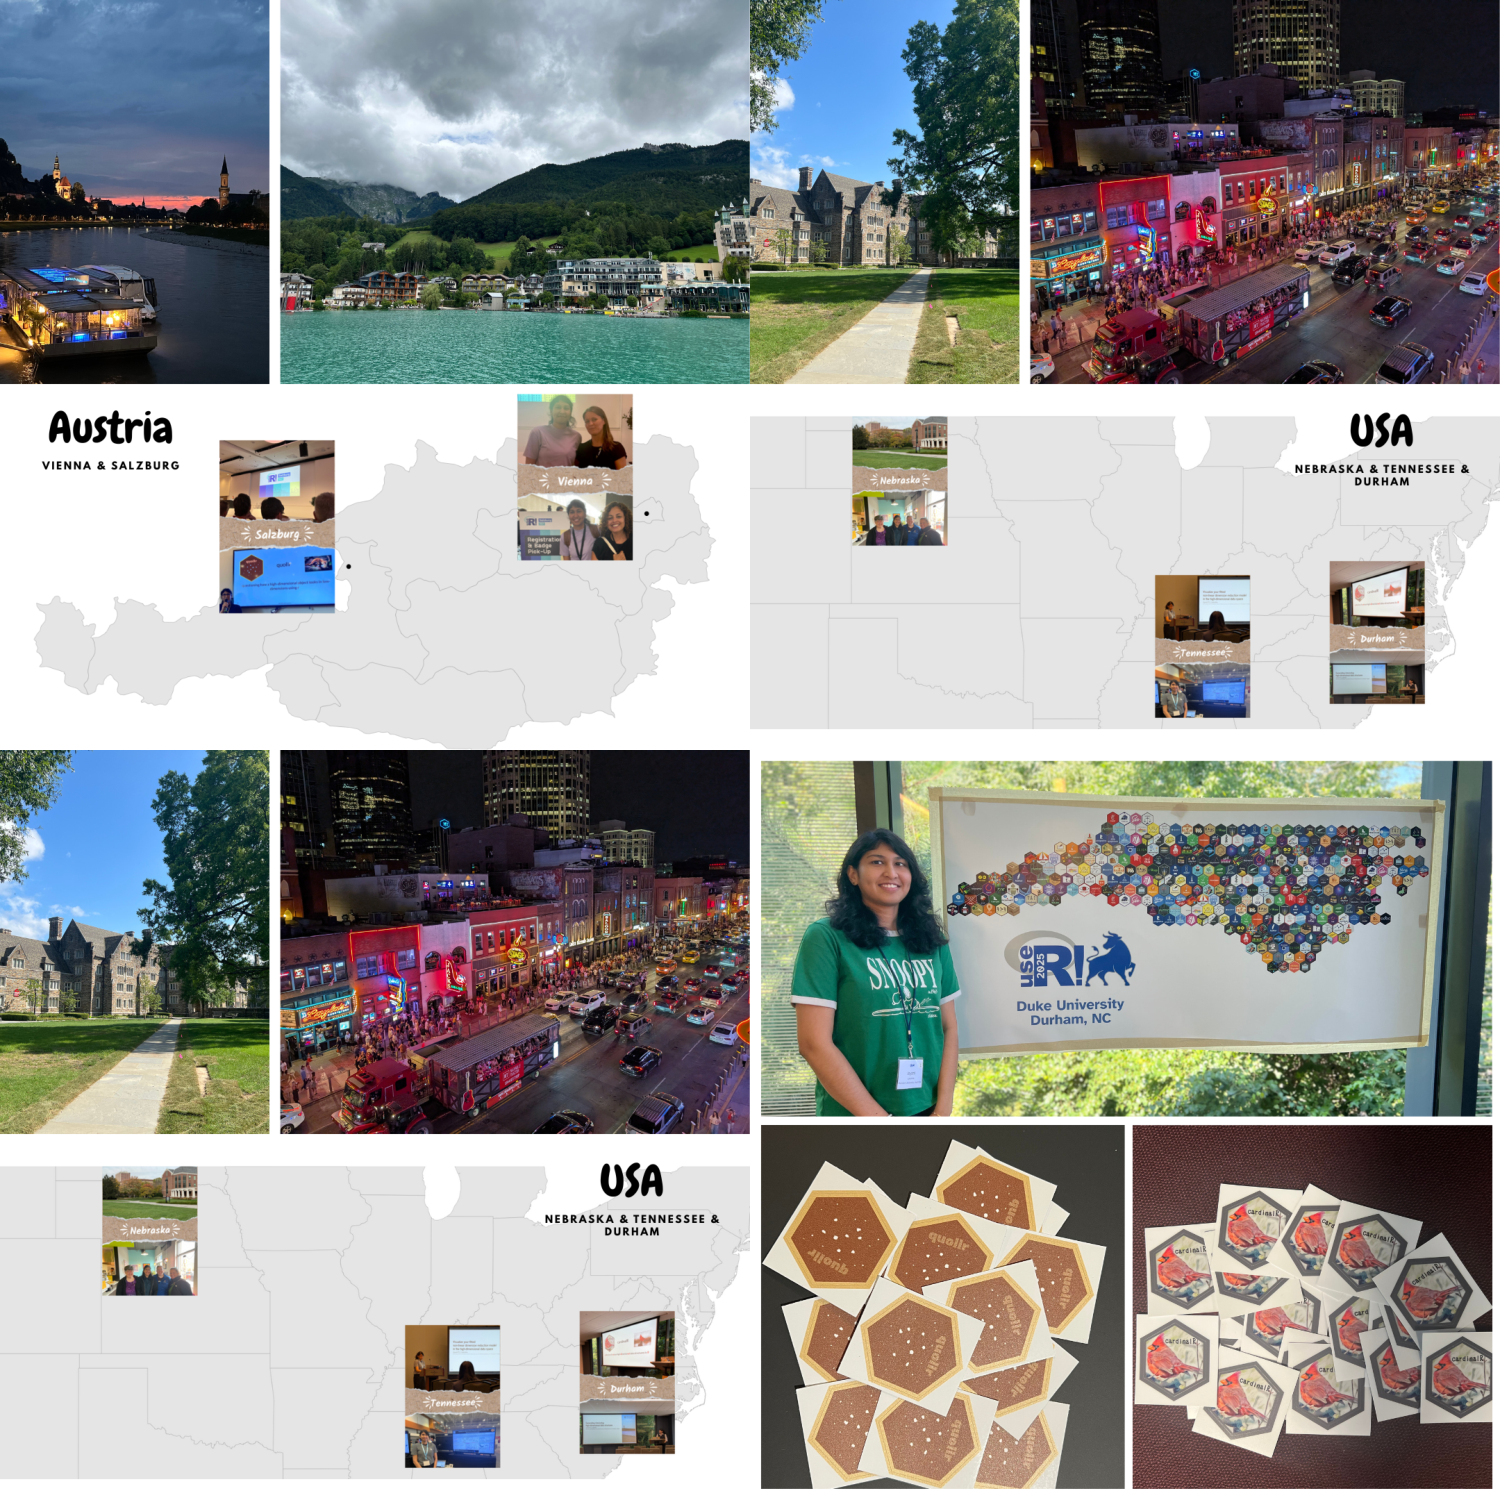
\includegraphics[keepaspectratio]{chapters/07-chap7_files/figure-pdf/unnamed-chunk-2-1.pdf}}

\clearpage

\bookmarksetup{startatroot}

\chapter*{Bibliography}\label{bibliography}
\addcontentsline{toc}{chapter}{Bibliography}

\markboth{Bibliography}{Bibliography}

\phantomsection\label{refs}
\begin{CSLReferences}{1}{0}
\bibitem[\citeproctext]{ref-jjallaire2024}
Allaire, J., and Dervieux, C. (2024),
\emph{\href{/url\%7Bhttps://CRAN.R-project.org/package=quarto\%7D.}{{quarto:
R Interface to Quarto Markdown Publishing System}}}.

\bibitem[\citeproctext]{ref-amid2022}
Amid, E., and Warmuth, M. K. (2022),
{``\href{https://arxiv.org/abs/1910.00204}{TriMap: Large-scale
dimensionality reduction using triplets}.''}

\bibitem[\citeproctext]{ref-As85}
Asimov, D. (1985), {``{T}he {G}rand {T}our: {A} {T}ool for {V}iewing
{M}ultidimensional {D}ata,''} \emph{SIAM Journal of Scientific and
Statistical Computing}, 6, 128--143.

\bibitem[\citeproctext]{ref-barber1996}
Barber, C. B., Dobkin, D. P., and Huhdanpaa, H. (1996),
{``\href{/url\%7Bhttps://doi.org/10.1145/235815.235821\%7D.}{{The
Quickhull Algorithm for Convex Hulls}},''} \emph{ACM Trans. Math.
Softw.}, 22, 469-\/-483.

\bibitem[\citeproctext]{ref-borg2005}
Borg, I., and Groenen, P. J. F. (2005),
\emph{\href{/url\%7Bhttps://doi.org/10.1007/0-387-28981-X\%7D.}{{Modern
Multidimensional Scaling}}}, New York, NY: Springer.

\bibitem[\citeproctext]{ref-brown2015}
Brown, T. A. (2015), \emph{{Confirmatory Factor Analysis for Applied
Research}}, New York, NY, US: {The Guilford Press}.

\bibitem[\citeproctext]{ref-carr1987}
Carr, D. B., Littlefield, R. J., Nicholson, W. L., and Littlefield, J.
S. (1987),
{``\href{/url\%7Bhttp://www.jstor.org/stable/2289444\%7D.}{{Scatterplot
Matrix Techniques for Large N}},''} \emph{Journal of the American
Statistical Association}, 82, 424--436.

\bibitem[\citeproctext]{ref-dan2023}
Carr, D., Lewin-Koh, N., Maechler, M., and Sarkar, D. (2023),
\emph{\href{/url\%7Bhttps://CRAN.R-project.org/package=hexbin\%7D.}{{hexbin:
Hexagonal Binning Routines}}}.

\bibitem[\citeproctext]{ref-chari2023}
Chari, T., and Pachter, L. (2023),
{``\href{https://doi.org/10.1371/journal.pcbi.1011288}{The specious art
of single-cell genomics},''} \emph{PLoS Computational Biology}, 19,
e1011288.

\bibitem[\citeproctext]{ref-chen2024}
Chen, Z., Wang, C., Huang, S., Shi, Y., and Xi, R. (2024),
{``\href{/url\%7Bhttps://www.sciencedirect.com/science/article/pii/S2667237524001735\%7D.}{{Directly
Selecting Cell-type Marker Genes for Single-cell Clustering
Analyses}},''} \emph{Cell Reports Methods}, 4, 100810.

\bibitem[\citeproctext]{ref-coifman2005}
Coifman, R. R., Lafon, S., Lee, A. B., Maggioni, M., Nadler, B., Warner,
F., and Zucker, S. W. (2005),
{``\href{/url\%7Bhttps://www.pnas.org/doi/abs/10.1073/pnas.0500334102\%7D.}{{Geometric
Diffusions as a Tool for Harmonic Analysis and Structure Definition of
Data: Diffusion Maps}},''} \emph{Proceedings of the National Academy of
Sciences of the United States of America}, 102, 7426--7431.

\bibitem[\citeproctext]{ref-freedman1981}
Freedman, D. A., and Diaconis, P. (1981),
{``\href{/url\%7Bhttps://doi.org/10.1007/BF01025868\%7D.}{{On the
Histogram as a Density Estimator: L2 Theory}},''} \emph{Probability
Theory and Related Fields}, 57, 453--476.

\bibitem[\citeproctext]{ref-alb2024}
Gebhardt, A., Bivand, R., and Sinclair, D. (2024),
\emph{\href{/url\%7Bhttps://CRAN.R-project.org/package=interp\%7D.}{{interp:
Interpolation Methods}}}.

\bibitem[\citeproctext]{ref-pbmc2019}
Genomics, 10x (2016),
{``\href{/url\%7Bhttps://www.10xgenomics.com/datasets/3-k-pbm-cs-from-a-healthy-donor-1-standard-1-1-0\%7D.}{{3k
PBMCs from a Healthy Donor, Universal 3' Gene Expression dataset
analysed using Cell Ranger 1.1.0}}.''}

\bibitem[\citeproctext]{ref-hao2021}
Hao, Y., Hao, S., Andersen-Nissen, E., Mauck, W. M., Zheng, S., Butler,
A., Lee, M. J., Wilk, A. J., Darby, C., Zager, M., Hoffman, P.,
Stoeckius, M., Papalexi, E., Mimitou, E. P., Jain, J., Srivastava, A.,
Stuart, T., Fleming, L. M., Yeung, B., Rogers, A. J., McElrath, J. M.,
Blish, C. A., Gottardo, R., Smibert, P., and Satija, R. (2021),
{``Integrated analysis of multimodal single-cell data,''} \emph{Cell},
184, 3573--3587.e29.
https://doi.org/\url{https://doi.org/10.1016/j.cell.2021.04.048}.

\bibitem[\citeproctext]{ref-haque2017}
Haque, A., Engel, J., Teichmann, S. A., and Lönnberg, T. (2017),
{``\href{/url\%7Bhttps://doi.org/10.1186/s13073-017-0467-4\%7D.}{{A
Practical Guide to Single-cell RNA-sequencing for Biomedical Research
and Clinical Applications}},''} \emph{Genome Medicine}, 9, 75.

\bibitem[\citeproctext]{ref-harisson2024}
Harrison, P. (2023),
{``\href{/url\%7Bhttps://doi.org/10.32614/RJ-2023-046\%7D.}{{langevitour:
Smooth Interactive Touring of High Dimensions, Demonstrated With
scRNA-Seq Data}},''} \emph{The R Journal}, 15, 206--219.

\bibitem[\citeproctext]{ref-hart2022}
Hart, C., and Wang, E. (2022),
\emph{\href{/url\%7Bhttps://casperhart.github.io/detourr/\%7D.}{{detourr:
Portable and Performant Tour Animations}}}.

\bibitem[\citeproctext]{ref-hinton2006}
Hinton, G. E., and Salakhutdinov, R. R. (2006), {``Reducing the
dimensionality of data with neural networks,''} \emph{Science}, American
Association for the Advancement of Science, 313, 504--507.
\url{https://doi.org/10.1126/science.1127647}.

\bibitem[\citeproctext]{ref-irizarry2024}
Irizarry, R. (2024), {``Biologists, stop putting UMAP plots in your
papers,''}
https://simplystatistics.org/posts/2024-12-23-biologists-stop-including-umap-plots-in-your-papers/.

\bibitem[\citeproctext]{ref-jia2022}
Jia, W., Sun, M., Lian, J., and Hou, S. (2022), {``Feature
dimensionality reduction: A review,''} \emph{Complex \& Intelligent
Systems}, 8, 2663--2693.
\url{https://doi.org/10.1007/s40747-021-00637-x}.

\bibitem[\citeproctext]{ref-johnstone2009}
Johnstone, I. M., and Titterington, D. M. (2009),
{``\href{/url\%7Bhttps://royalsocietypublishing.org/doi/abs/10.1098/rsta.2009.0159\%7D.}{{Statistical
Challenges of High-Dimensional Data}},''} \emph{Philosophical
Transactions of the Royal Society A: Mathematical, Physical and
Engineering Sciences}, 367, 4237--4253.

\bibitem[\citeproctext]{ref-jolliffe2011}
Jolliffe, I. (2011),
{``\href{/url\%7Bhttps://doi.org/10.1007/978-3-642-04898-2_455\%7D.}{{Principal
Component Analysis}},''} in \emph{International encyclopedia of
statistical science}, Berlin, Heidelberg: Springer Berlin Heidelberg,
pp. 1094--1096.

\bibitem[\citeproctext]{ref-joreskog1969}
Jöreskog, K. G. (1969),
{``\href{/url\%7Bhttps://doi.org/10.1007/BF02289343\%7D.}{{A General
Approach to Confirmatory Maximum Likelihood Factor Analysis}},''}
\emph{Psychometrika}, 34, 183--202.

\bibitem[\citeproctext]{ref-tomasz2023}
Konopka, T. (2023),
\emph{\href{/url\%7Bhttps://CRAN.R-project.org/package=umap\%7D.}{{umap:
Uniform Manifold Approximation and Projection}}}.

\bibitem[\citeproctext]{ref-jesse2015}
Krijthe, J. H. (2015),
\emph{\href{/url\%7Bhttps://github.com/jkrijthe/Rtsne\%7D.}{{Rtsne:
T-Distributed Stochastic Neighbor Embedding Using Barnes-Hut
Implementation}}}.

\bibitem[\citeproctext]{ref-kruskal1964}
Kruskal, J. B. (1964),
{``\href{/url\%7Bhttps://doi.org/10.1007/BF02289694\%7D.}{{Nonmetric
Multidimensional Scaling: A Numerical Method}},''} \emph{Psychometrika},
29, 115--129.

\bibitem[\citeproctext]{ref-laa2022}
Laa, U., Cook, D., and Lee, S. (2022),
{``\href{/url\%7Bhttps://doi.org/10.1080/10618600.2021.1963264\%7D.}{{Burning
Sage: Reversing the Curse of Dimensionality in the Visualization of
High-Dimensional Data}},''} \emph{Journal of Computational and Graphical
Statistics}, 31, 40--49.

\bibitem[\citeproctext]{ref-stephane2023}
Laurent, S. (2023),
\emph{\href{/url\%7Bhttps://github.com/stla/cxhull\%7D.}{{cxhull: Convex
Hull}}}.

\bibitem[\citeproctext]{ref-lecun1998}
LeCun, Y., Cortes, C., and Burges, C. J. C. (1998),
{``\href{/url\%7Bhttp://yann.lecun.com/exdb/mnist/\%7D.}{{The MNIST
Database of Handwritten Digits}}.''}

\bibitem[\citeproctext]{ref-lee1980}
Lee, D. T., and Schachter, B. J. (1980),
{``\href{/url\%7Bhttps://doi.org/10.1007/BF00977785\%7D.}{{Two
Algorithms For Constructing a Delaunay Triangulation}},''}
\emph{International Journal of Computer \& Information Sciences}, 9,
219--242.

\bibitem[\citeproctext]{ref-john2015}
Lee, J. A., Peluffo-Ordóñez, D. H., and Verleysen, M. (2015),
{``Multi-scale similarities in stochastic neighbour embedding: Reducing
dimensionality while preserving both local and global structure,''}
\emph{Neurocomputing}, 169, 246--261.
https://doi.org/\url{https://doi.org/10.1016/j.neucom.2014.12.095}.

\bibitem[\citeproctext]{ref-lee2021}
Lee, S., Cook, D., Silva, N. da, Laa, U., Wang, E., Spyrison, N., and
Zhang, H. S. (2021), {``{A Review of the State-of-the-Art on Tours for
Dynamic Visualization of High-Dimensional Data},''} \emph{arXiv preprint
arXiv:2104.08016}.

\bibitem[\citeproctext]{ref-laurens2008}
Maaten, L. V. D., and Hinton, G. E. (2008),
{``\href{/url\%7Bhttps://api.semanticscholar.org/CorpusID:5855042\%7D.}{{Visualizing
Data Using t-SNE}},''} \emph{Journal of Machine Learning Research}, 9,
2579--2605.

\bibitem[\citeproctext]{ref-van2009}
Maaten, L. van der (2009), {``Learning a parametric embedding by
preserving local structure,''} in \emph{Artificial intelligence and
statistics}, PMLR, pp. 384--391.

\bibitem[\citeproctext]{ref-leland2018}
McInnes, L., Healy, J., Saul, N., and Großberger, L. (2018),
{``\href{/url\%7Bhttps://doi.org/10.21105/joss.00861\%7D.}{{UMAP:
Uniform Manifold Approximation and Projection}},''} \emph{Journal of
Open Source Software}, 3, 861.

\bibitem[\citeproctext]{ref-moon2019}
Moon, K. R., Dijk, D. van, Wang, Z., Gigante, S. A., Burkhardt, D. B.,
Chen, W. S., Yim, K., Elzen, A. van den, Hirn, M. J., Coifman, R. R.,
Ivanova, N. B., Wolf, G., and Krishnaswamy, S. (2019),
{``\href{/url\%7Bhttps://doi.org/10.1038/s41587-019-0336-3\%7D.}{{Visualizing
Structure and Transitions in High-Dimensional Biological Data}},''}
\emph{Nature Biotechnology}, 37, 1482--1492.

\bibitem[\citeproctext]{ref-thomas2024}
Pedersen, T. L. (2024),
\emph{\href{/url\%7Bhttps://CRAN.R-project.org/package=patchwork\%7D.}{{patchwork:
The Composer of Plots}}}.

\bibitem[\citeproctext]{ref-saeed2018}
Saeed, N., Nam, H., Haq, M. I. U., and Muhammad Saqib, D. B. (2018),
{``\href{/url\%7Bhttps://doi.org/10.1145/3178155\%7D.}{{A Survey on
Multidimensional Scaling}},''} \emph{ACM Comput. Surv.}, 51.

\bibitem[\citeproctext]{ref-shepard1962}
Shepard, R. N. (1962), {``The analysis of proximities: Multidimensional
scaling with an unknown distance function. i.''} \emph{Psychometrika},
27, 125--140. \url{https://doi.org/10.1007/BF02289630}.

\bibitem[\citeproctext]{ref-silva2002}
Silva, V., and Tenenbaum, J. (2002),
{``\href{/url\%7Bhttps://proceedings.neurips.cc/paper_files/paper/2002/file/5d6646aad9bcc0be55b2c82f69750387-Paper.pdf\%7D.}{{Global
Versus Local Methods in Nonlinear Dimensionality Reduction}},''}
\emph{Advances in Neural Information Processing Systems}, 15, 721--728.

\bibitem[\citeproctext]{ref-spearman1961}
Spearman, C. (1961), {``The proof and measurement of association between
two things.''} Appleton-Century-Crofts.

\bibitem[\citeproctext]{ref-kevin2024}
Ushey, K., Allaire, J., and Tang, Y. (2024),
\emph{\href{/url\%7Bhttps://CRAN.R-project.org/package=reticulate\%7D.}{{reticulate:
Interface to Python}}}.

\bibitem[\citeproctext]{ref-yingfan2021}
Wang, Y., Huang, H., Rudin, C., and Shaposhnik, Y. (2021),
{``\href{/url\%7Bhttp://jmlr.org/papers/v22/20-1061.html\%7D.}{{Understanding
How Dimension Reduction Tools Work: An Empirical Approach to Deciphering
t-SNE, UMAP, TriMap, and PaCMAP for Data Visualization}},''}
\emph{Journal of Machine Learning Research}, 22, 1--73.

\bibitem[\citeproctext]{ref-hadley2023}
Wickham, H. (2023),
\emph{\href{/url\%7Bhttps://CRAN.R-project.org/package=conflicted\%7D.}{{conflicted:
An Alternative Conflict Resolution Strategy}}}.

\bibitem[\citeproctext]{ref-hadley2019}
Wickham, H., Averick, M., Bryan, J., Chang, W., McGowan, L. D.,
François, R., Grolemund, G., Hayes, A., Henry, L., Hester, J., Kuhn, M.,
Pedersen, T. L., Miller, E., Bache, S. M., Müller, K., Ooms, J.,
Robinson, D., Seidel, D. P., Spinu, V., Takahashi, K., Vaughan, D.,
Wilke, C., Woo, K., and Yutani, H. (2019),
{``\href{/url\%7Bhttps://doi.org/10.21105/joss.01686\%7D.}{{Welcome to
the Tidyverse}},''} \emph{Journal of Open Source Software}, 4, 1686.

\bibitem[\citeproctext]{ref-wickham2015}
Wickham, H., Cook, D., and Hofmann, H. (2015),
{``\href{/url\%7Bhttps://onlinelibrary.wiley.com/doi/abs/10.1002/sam.11271\%7D.}{{Visualizing
Statistical Models: Removing the Blindfold}},''} \emph{Statistical
Analysis and Data Mining: The ASA Data Science Journal}, 8, 203--225.

\bibitem[\citeproctext]{ref-wickham2011}
Wickham, H., Cook, D., Hofmann, H., and Buja, A. (2011),
{``\href{/url\%7Bhttp://www.jstatsoft.org/v40/i02/\%7D.}{{tourr: An R
Package For Exploring Multivariate Data With Projections}},''}
\emph{Journal of Statistical Software}, 40, 1--18.

\bibitem[\citeproctext]{ref-xia2023}
Xia, L., Lee, C., and Li, J. J. (2023),
{``\href{/url\%7Bhttps://www.biorxiv.org/content/early/2023/04/25/2023.04.21.537839\%7D.}{{scDEED:
A Statistical Method for Detecting Dubious 2D Single-cell
Embeddings}},''} \emph{bioRxiv}.

\bibitem[\citeproctext]{ref-achim2020}
Zeileis, A., Fisher, J. C., Hornik, K., Ihaka, R., McWhite, C. D.,
Murrell, P., Stauffer, R., and Wilke, C. O. (2020),
{``\href{/url\%7Bhttps://www.jstatsoft.org/index.php/jss/article/view/v096i01\%7D.}{{colorspace:
A Toolbox for Manipulating and Assessing Colors and Palettes}},''}
\emph{Journal of Statistical Software}, 96, 1--49.

\bibitem[\citeproctext]{ref-hao2024}
Zhu, H. (2024),
\emph{\href{/url\%7Bhttps://CRAN.R-project.org/package=kableExtra\%7D.}{{kableExtra:
Construct Complex Table with kable and Pipe Syntax}}}.

\end{CSLReferences}

\cleardoublepage
\phantomsection
\addcontentsline{toc}{part}{Appendices}
\appendix

\chapter{Glossary}\label{glossary}

\begin{table}[H]

\caption{\label{tbl-glossary}Glossary.}

\centering{

\centering\begingroup\fontsize{12}{14}\selectfont

\begin{tabular}{>{\raggedright\arraybackslash}p{3cm}>{\raggedright\arraybackslash}p{12cm}}
\toprule
\textbf{Term} & \textbf{Description}\\
\midrule
Dimension reduction & NA\\
Embedding & NA\\
High-dimensional data & NA\\
Hyper_parameters & NA\\
Interactive graphics & NA\\
Layout/ representation & NA\\
Linear dimension reduction & NA\\
NLDR model & NA\\
Nonlinear dimension reduction (NLDR) techniques/ methods & NA\\
Uniform Manifold Approximation and Projection (UMAP) & A manifold learning-based NLDR technique preserving both local and some global structures efficiently.\\
large-scale dimensionality reduction using triplets (TriMAP) & NA\\
pairwise controlled manifold approximation (PaCMAP) & NA\\
potential of heat-diffusion for affinity-based trajectory embedding (PHATE) algorithm & NA\\
t-distributed stochastic neighbor embedding (tSNE) & NA\\
tour & NA\\
\bottomrule
\end{tabular}
\endgroup{}

}

\end{table}%

\chapter{Appendix to ``Choosing Better NLDR Layouts by Evaluating the
Model in the High-dimensional Data Space''}\label{sec-appendix-a}

\section{Methods and hyper-parameters used to generate
layouts}\label{methods-and-hyper-parameters-used-to-generate-layouts}

Table~\ref{tbl-fig-param} contains the list of methods and
hyper-parameters used for each of the layouts shown in the paper.

\begingroup\fontsize{12}{14}\selectfont

\begin{longtable}{>{\raggedright\arraybackslash}p{1.5cm}>{\raggedright\arraybackslash}p{2cm}>{\raggedright\arraybackslash}p{10cm}}

\caption{\label{tbl-fig-param}NLDR methods and hyper-parameters used for
each Figure in the main paper.}

\tabularnewline

\toprule
\textbf{Figure} & \textbf{NLDR method} & \textbf{Hyper-parameter(s)}\\
\midrule
\endfirsthead
\multicolumn{3}{@{}l}{\textit{(continued)}}\\
\toprule
\textbf{Figure} & \textbf{NLDR method} & \textbf{Hyper-parameter(s)}\\
\midrule
\endhead

\endfoot
\bottomrule
\endlastfoot
$1$a & UMAP & n\_neighbors = 30, min\_dist = 0.3\\
$1$b & UMAP & n\_neighbors = 5, min\_dist = 0.8\\
$1$c & UMAP & n\_neighbors = 5, min\_dist = 0.01\\
$1$d & tSNE & perplexity = 5\\
$1$e & tSNE & perplexity = 30\\
$1$f & PHATE & knn = 5\\
$1$g & TriMAP & n\_inliers = 12, n\_outliers = 4, n\_random = 3\\
$1$h & PaCMAP & n\_neighbors = 30, init = random, MN\_ratio = 0.9, FP\_ratio = 5\\
\midrule
$2$ & tSNE & perplexity = 47\\
$4$a & tSNE & perplexity = 47\\
$5$b & tSNE & perplexity = 47\\
$6$ & tSNE & perplexity = 47\\
\midrule
$8$a & tSNE & perplexity = 47\\
$8$b & tSNE & perplexity = 62\\
$8$c & UMAP & n\_neighbors = 15, min\_dist = 0.1\\
$8$d & PHATE & knn = 5\\
$8$e & TriMAP & n\_inliers = 12, n\_outliers = 4, n\_random = 3\\
$8$f & PaCMAP & n\_neighbors = 10, init = random, MN\_ratio = 0.5, FP\_ratio = 2\\
\midrule
$10$a & UMAP & n\_neighbors = 30, min\_dist = 0.3\\
$10$b & UMAP & n\_neighbors = 5, min\_dist = 0.8\\
$10$c & UMAP & n\_neighbors = 5, min\_dist = 0.01\\
$10$d & tSNE & perplexity = 5\\
$10$e & tSNE & perplexity = 30\\
$10$f & PHATE & knn = 5\\
$10$g & TriMAP & n\_inliers = 12, n\_outliers = 4, n\_random = 3\\
$10$h & PaCMAP & n\_neighbors = 30, init = random, MN\_ratio = 0.9, FP\_ratio = 5\\
\midrule
$11$a & UMAP & n\_neighbors = 30, min\_dist = 0.3\\
$11$e & tSNE & perplexity = 30\\
\midrule
$12$a & tSNE & perplexity = 30\\
$12$b & tSNE & perplexity = 89\\
$12$c & UMAP & n\_neighbors = 15, min\_dist = 0.1\\
$12$d & PHATE & knn = 5\\
$12$e & TriMAP & n\_inliers = 12, n\_outliers = 4, n\_random = 3\\
$12$f & PaCMAP & n\_neighbors = 10, init = random, MN\_ratio = 0.5, FP\_ratio = 2\\
\midrule
$13$a & tSNE & perplexity = 30\\
\midrule
$14$a & tSNE & perplexity = 30\\
\midrule
$A4$a & tSNE & perplexity = 71\\
$A4$b & UMAP & n\_neighbors = 15, min\_dist = 0.1\\
$A4$c & PaCMAP & n\_neighbors = 10, init = random, MN\_ratio = 0.5, FP\_ratio = 2\\
\midrule
$A5$ & tSNE & perplexity = 52\\
\midrule
$A6$a & UMAP & n\_neighbors = 30, min\_dist = 0.3\\
$A6$b & tSNE & perplexity = 30\\
\midrule
$A7$a & UMAP & n\_neighbors = 30, min\_dist = 0.3\\
$A7$b & tSNE & perplexity = 30\\
\midrule
$A8$a & UMAP & n\_neighbors = 30, min\_dist = 0.3\\
$A8$b & tSNE & perplexity = 30\\
\midrule
$A9$a & UMAP & n\_neighbors = 30, min\_dist = 0.3\\
$A9$b & UMAP & n\_neighbors = 5, min\_dist = 0.8\\
$A9$c & UMAP & n\_neighbors = 5, min\_dist = 0.01\\
$A9$d & tSNE & perplexity = 5\\
$A9$e & tSNE & perplexity = 30\\
$A9$f & PHATE & knn = 5\\
$A9$g & TriMAP & n\_inliers = 12, n\_outliers = 4, n\_random = 3\\
$A9$h & PaCMAP & n\_neighbors = 30, init = random, MN\_ratio = 0.9, FP\_ratio = 5\\
\midrule
$A10$a & tSNE & perplexity = 30\\
$A10$b & tSNE & perplexity = 89\\
$A10$c & UMAP & n\_neighbors = 15, min\_dist = 0.1\\
$A10$d & PHATE & knn = 5\\
$A10$e & TriMAP & n\_inliers = 12, n\_outliers = 4, n\_random = 3\\
$A10$f & PaCMAP & n\_neighbors = 10, init = random, MN\_ratio = 0.5, FP\_ratio = 2\\*

\end{longtable}

\endgroup{}

\section{Videos links}\label{videos-links}

Animations of the \pD{} tours that produced specific projections shown
in some figures in the main paper are available on YouTube at the links
given in Table~\ref{tbl-links}.

\begin{table}[H]

\caption{\label{tbl-links}Videos of the langevitour animations and the
linked plots.}

\centering{

\centering\begingroup\fontsize{12}{14}\selectfont

\begin{tabular}{>{\raggedright\arraybackslash}p{1.5cm}>{\raggedright\arraybackslash}p{14cm}}
\toprule
\textbf{Figure} & \textbf{URL}\\
\midrule
$4$ & \href{https://youtu.be/yHKTHK4UBiU}{\texttt{youtu.be/yHKTHK4UBiU}}\\
$5$ & \href{https://youtu.be/FukiminrO90}{\texttt{youtu.be/FukiminrO90}}\\
$11$ & \href{https://youtu.be/3VfK3M2gnZM}{\texttt{youtu.be/3VfK3M2gnZM}}, \href{https://youtu.be/Es84bwQcndU}{\texttt{youtu.be/Es84bwQcndU}}\\
$13$ & \href{https://youtu.be/sUcGd57Swdg}{\texttt{youtu.be/sUcGd57Swdg}}, \href{https://youtu.be/QiklCjELUxo}{\texttt{youtu.be/QiklCjELUxo}}\\
\bottomrule
\end{tabular}
\endgroup{}

}

\end{table}%

\section{Notation}\label{notation}

\begin{table}[H]

\caption{\label{tbl-notation}Summary of notation for describing new
methodology.}

\centering{

\centering\begingroup\fontsize{12}{14}\selectfont

\begin{tabular}{>{\raggedright\arraybackslash}p{3cm}>{\raggedright\arraybackslash}p{12cm}}
\toprule
\textbf{Notation} & \textbf{Description}\\
\midrule
$n, p, k$ & number of observations, variables, embedding dimension, respectively\\
$\mathbfit{X}, \mathbfit{x}$ & $p$-dimensional data (population, sample)\\
$\mathbfit{y}$ & $k$-dimensional layout\\
$P$ & orthonormal basis, generating a $d\text{-}dimensional$ linear projection of $p$-dimensional data\\
$T$ & true  model\\
$g$ & functional mapping from \pD{} to \kD{}, especially as prescribed by NLDR\\
$\mathbfit{\theta}$ & (Hyper-) parameters for NLDR method\\
$r$ & ranges of the embedding components\\
$C^{(j)}$ & $j$-dimensional bin centers\\
$(b_1, b_2)$ & number of bins in each direction\\
$(a_1, a_2)$ & binwidths, distance between centroids in each direction\\
$(s_1, \ s_2)$ & starting coordinates of the hexagonal grid\\
$q$ & buffer to ensure hexgrid covers data, proportion of data range, 0-1\\
$m$ & number of non-empty bins\\
$b$ & number of  hexagons in the grid\\
$h$ & hexagonal id\\
$l$ & side length\\
$A$ & area\\
$n_h$ & number of points in hexagon $h$ (bin count)\\
$w_h$ & standardized number of points in hexagon $h$ (standardized bin counts)\\
$d_h$ & density of hexagon $h$ (bin density)\\
\bottomrule
\end{tabular}
\endgroup{}

}

\end{table}%

\section{Scripts}\label{scripts}

\begingroup\fontsize{12}{14}\selectfont

\begin{longtable}{>{\raggedright\arraybackslash}p{3.5cm}>{\raggedright\arraybackslash}p{6.5cm}>{\raggedright\arraybackslash}p{3cm}}

\caption{\label{tbl-script-desc}R and Python script files used to
generate outputs in the main paper.}

\tabularnewline

\toprule
\textbf{Folder} & \textbf{Script} & \textbf{Description}\\
\midrule
\endfirsthead
\multicolumn{3}{@{}l}{\textit{(continued)}}\\
\toprule
\textbf{Folder} & \textbf{Script} & \textbf{Description}\\
\midrule
\endhead

\endfoot
\bottomrule
\endlastfoot
script & additional\_functions.R & Helper functions to render the main paper.\\
script & evaluation.py & Python script implementing additional evaluation metrics such as RTA and GS.\\
script & nldr\_code.R & Wrapper functions for running multiple NLDR methods (UMAP, tSNE, PHATE, PaCMAP, TriMAP) with different parameters.\\
\midrule
two\_nonlinear & 01\_gen\_data.R & Generates the 2NC7 dataset.\\
two\_nonlinear & 02\_gen\_true\_model.R & Creates the true structure of 2NC7 data.\\
two\_nonlinear & 03\_gen\_embeddings.R & Computes multiple NLDR embeddings for the 2NC7 data.\\
two\_nonlinear & 04\_gen\_mse\_for\_diff\_methods.R & Computes HBE with varying bin widths ($a_1$) for all NLDR embeddings.\\
two\_nonlinear & 05\_gen\_rm\_lwd\_mse.R & Computes HBE with varying low density bin cutoff for all three binwidth ($a_1$) choices.\\
two\_nonlinear & 06\_gen\_model\_with\_tSNE.R & Fits the model for the layout a.\\
two\_nonlinear & 07\_example\_evaluation\_metrics.R & Calculates evaluation metrics for all NLDR layouts.\\
two\_nonlinear & 08\_gen\_model\_with\_PHATE.R & Fits the model for the layout c.\\
\midrule
five\_gau\_clusters & 01\_five\_gaussian\_cluster\_data\_emb.R & Generates data and multiple NLDR embeddings.\\
five\_gau\_clusters & 02\_gen\_model\_with\_tSNE.R & Fits the model for the layout a.\\
five\_gau\_clusters & 03\_gen\_model\_with\_UMAP.R & Fits the model for the layout b.\\
five\_gau\_clusters & 04\_gen\_model\_with\_PaCMAP.R & Fits the model for the layout c.\\
\midrule
c\_shaped\_dens\_str & 01\_gen\_data.R & Generates the $2\text{-}D$ curved sheet dataset.\\
c\_shaped\_dens\_str & 02\_gen\_embeddings\_uni\_dens.R & Generates multiple NLDR embeddings.\\
c\_shaped\_dens\_str & 03\_gen\_model\_with\_tSNE.R & Fits the model for the tSNE layout.\\
\midrule
pbmc3k & 01\_obtain\_pca\_author.R & Obtains  author\'s PCA results.\\
pbmc3k & 02\_obtain\_umap\_authors.R & Obtains  author\'s UMAP embeddings.\\
pbmc3k & 03\_gen\_umap\_diff\_param.R & Generates multiple UMAP embeddings with different hyper\-parameter values.\\
pbmc3k & 04\_gen\_tsne\_diff\_param.R & Generates multiple tSNE embeddings with different hyper\-parameter values.\\
pbmc3k & 05\_gen\_phate.R & Generates a PHATE embeddings with default hyper\-parameters.\\
pbmc3k & 06\_gen\_trimap.R & Generates a TriMAP embeddings with default hyper\-parameters.\\
pbmc3k & 07\_gen\_pacmap.R & Generates a PaCMAP embeddings with default hyper\-parameters.\\
pbmc3k & 08\_gen\_mse\_for\_diff\_methods.R & Computes HBE with varying bin widths ($a_1$) for all NLDR embeddings.\\
pbmc3k & 09\_gen\_scDEED.R & Generates UMAP embeddings from scDEED results.\\
pbmc3k & 10\_pre\_process\_for\_embedding.R & Generates PBMC3k data used for scDEED results.\\
pbmc3k & 11\_gen\_mse\_for\_diff\_tsne\_scD.R & Computes HBE with varying bin widths ($a_1$) for tSNE embeddings.\\
pbmc3k & 12\_gen\_mse\_for\_diff\_umap\_scD.R & Computes HBE with varying bin widths ($a_1$) for UMAP embeddings.\\
pbmc3k & 13\_gen\_model\_with\_UMAP.R & Fits the model for the layout a.\\
pbmc3k & 14\_gen\_model\_with\_tSNE.R & Fits the model for the layout e.\\
pbmc3k & 15\_gen\_model\_with\_UMAP\_scD.R & Fits the model for the layout a.\\
pbmc3k & 16\_gen\_model\_with\_tSNE\_scD.R & Fits the model for the layout b.\\
pbmc3k & 17\_evaluation\_metrics.R & Calculates evaluation metrics for all NLDR layouts.\\
pbmc3k & 18\_evaluation\_metrics\_scD.R & Calculates evaluation metrics for all NLDR layouts.\\
\midrule
mnist & 01\_data\_preprocessing.R & Computes first $10$ principal components and save data.\\
mnist & 02\_gen\_diff\_embeddings.R & Generates multiple NLDR embeddings.\\
mnist & 03\_gen\_mse\_for\_diff\_methods.R & Computes HBE with varying bin widths ($a_1$) for all NLDR embeddings.\\
mnist & 04\_gen\_model\_with\_tSNE.R & Fits the model for the layout a.\\
mnist & 05\_evaluation\_metrics.R & Calculates evaluation metrics for all NLDR layouts.\\
mnist & 06\_link\_brush\_layout\_e.R & Creates interactive linked brushing with layout e.\\*

\end{longtable}

\endgroup{}

\section{Generating the 2NC7 data}\label{generating-the-2nc7-data}

This data is constructed by simulating two clusters, each consisting of
\(1000\) observations. The C-shaped cluster is generated from
\(\theta \sim U(\text{-}3\pi/2, 0)\), \(X_1 = \sin(\theta)\),
\(X_2 \sim U(0, 2)\) (adding thickness to the C),
\(X_3 = \text{sign}(\theta) \times (\cos(\theta) - 1)\),
\(X_4 = \cos(\theta)\). Observations lie on a \gD{} manifold in \sD{}.
The other cluster is from \(X_1 \sim U(0, 2)\), \(X_2 \sim U(0, 3)\),
\(X_3 = \text{-}(X_1^3 + X_2)\), and \(X_4 \sim U(0, 2)\). It is also
curved, but observations lie on a \tD{} manifold in\sD{}. Three more
variables, \(X_5, X_6, X_7\), that are small amounts of pure noise are
added. We would consider \(T=(X_1, X_2, X_3, X_4)\) to be the geometric
structure (true model) that we hope to capture.

\begin{figure}[H]

{\centering 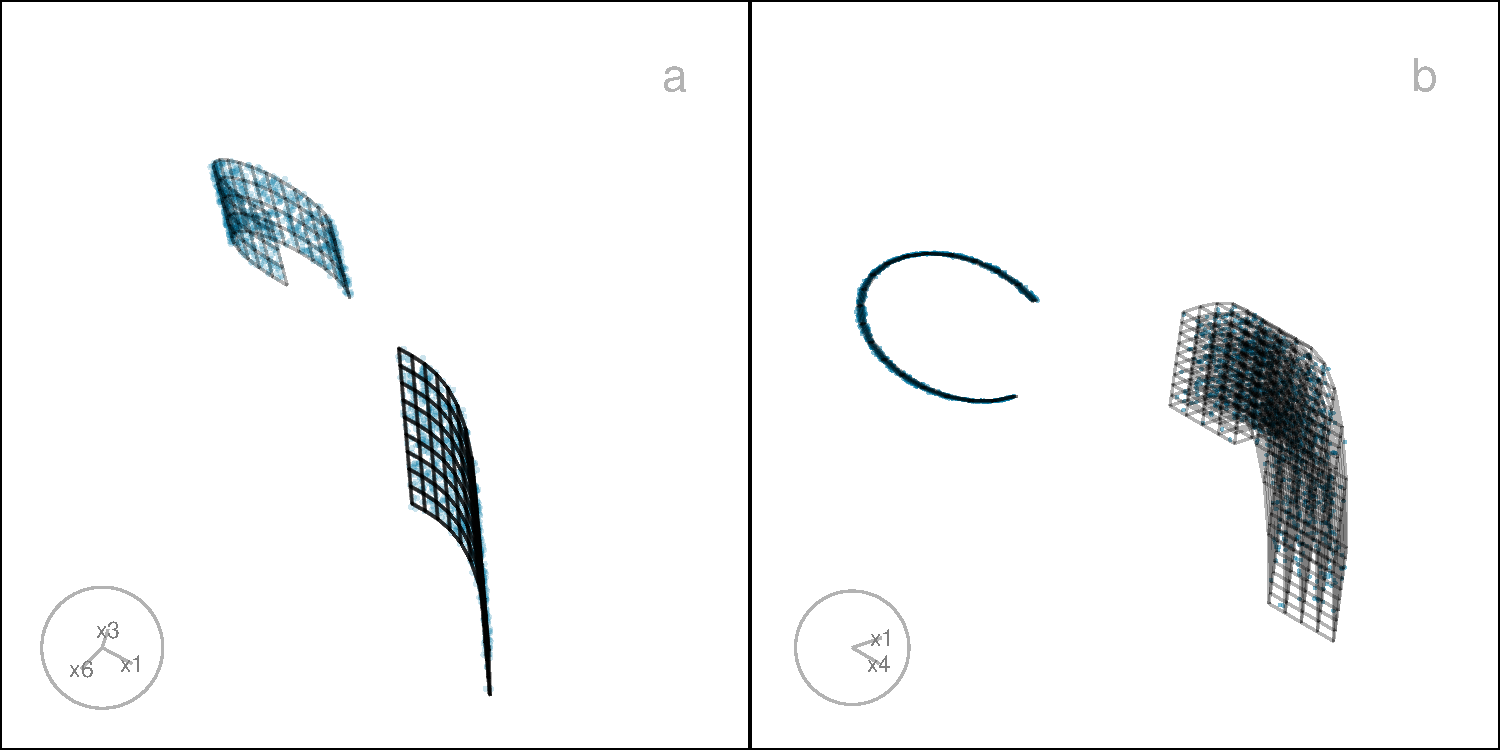
\includegraphics[width=1\linewidth,height=\textheight,keepaspectratio]{appendix/B-appB_files/figure-pdf/unnamed-chunk-4-1.pdf}

}

\caption{Two projections of the \pD{} true model overlaying the data are
shown in a, b. Video of the langevitour animations is available at
\url{https://youtu.be/35TrnYJsUUI}.}

\end{figure}%

\section{Computing hexagon grid
configurations}\label{computing-hexagon-grid-configurations}

Given range of embedding component, \(r_2\), number of bins along the
x-axis, \(b_1\), and buffer proportion, \(q\), hexagonal starting point
coordinates, \(s_1 = \text{-}q\), and \(s_2 = \text{-}qr_2\). The
purpose is to find width of the hexagon. \(a_1\), and number of bins
along the y-axis, \(b_2\).

Geometric arguments give rise to the following constraints.

\(\text{min }a_1 \text{ s.t.}\)

\begin{equation}\phantomsection\label{eq-equation1}{
s_1 - \frac{a_1}{2} < 0,
}\end{equation}

\begin{equation}\phantomsection\label{eq-equation2}{
s_1 + (b_1 - 1) \times a_1 \geq 1,
}\end{equation}

\begin{equation}\phantomsection\label{eq-equation4}{
s_2 - \frac{a_2}{2} < 0,
}\end{equation}

\begin{equation}\phantomsection\label{eq-equation5}{
s_2 + (b_2 - 1) \times a_2 \geq r_2.
}\end{equation}

Since \(a_1\) and \(a_2\) are distances,

\[
a_1, a_2 > 0.
\] Also, \((s_1, s_2) \in (\text{-}0.1, \text{-}0.05)\) as these are
multiplicative offsets in the negative direction.

Equation~\ref{eq-equation1} can be rearranged as,

\[
a_1 > 2s_1
\]

which given \(s_1 < 0\) and \(a_1 > 0\) will \emph{always} be true. The
same logic follows for Equation~\ref{eq-equation4} and substituting
\(a_2 = \sqrt{3}a_1/{2}\), and \(s_2 = \text{-}qr_2\) to
Equation~\ref{eq-equation4} can be written as,

\[
a_1 > -\frac{4}{\sqrt{3}}qr_2
\]

Also, substituting \(a_2 = \sqrt{3}a_1/{2}\), \(s_2 = \text{-}qr_2\) and
rearranging Equation~\ref{eq-equation5} gives:

\begin{equation}\phantomsection\label{eq-equation6}{
a_1 \geq \frac{2(r_2 + qr_2)}{\sqrt{3}(b_2 - 1)}.
}\end{equation}

Similarly, substituting \(s_1 = \text{-}q\) Equation~\ref{eq-equation2}
becomes,

\begin{equation}\phantomsection\label{eq-equation7}{
a_1 \geq \frac{(1 + q)}{(b_1 - 1)}.
}\end{equation}

This is a linear optimization problem. Therefore, the optimal solution
must occur on a vertex. So, by setting Equation~\ref{eq-equation6}
equals to Equation~\ref{eq-equation7} gives,

\[
\frac{2(r_2 + qr_2)}{\sqrt{3}(b_2 - 1)} = \frac{(1 + q)}{(b_1 - 1)}.
\]

After rearranging this,

\[
b_2 = 1 + \frac{2r_2(b_1 - 1)}{\sqrt{3}}
\]

and since \(b_2\) should be an integer,

\begin{equation}\phantomsection\label{eq-equation8}{
b_2 = \Big\lceil1 +\frac{2r_2(b_1 - 1)}{\sqrt{3}}\Big\rceil.
}\end{equation}

Furthermore, with known \(b_1\) and \(b_2\), by considering
Equation~\ref{eq-equation2} or Equation~\ref{eq-equation5} as the
\emph{binding} or \emph{active constraint}, can compute \(a_1\).

If Equation~\ref{eq-equation2} is active, then,

\[
\frac{(1 + q)}{(b_1 - 1)} < \frac{2(r_2 + qr_2)}{\sqrt{3}(b_2 - 1)}.
\]

Rearranging this gives,

\[
r_2 > \frac{\sqrt{3}(b_2 - 1)}{2(b_1 - 1)}.
\]

Therefore, if this equality is true, then \[
a_1 = \frac{(1+q)}{(b_1 - 1)},
\] otherwise, \[
a_1 = \frac{2r_2(1+q)}{\sqrt{3}(b_2 - 1)}.
\]

\section{Binning the data}\label{binning-the-data-2}

Points are assigned to the bin they fall into based on the nearest
centroid. If a point is equidistant from multiple centroids, it is
assigned to the centroid with the smallest bin ID.

\begin{figure}[H]

\centering{

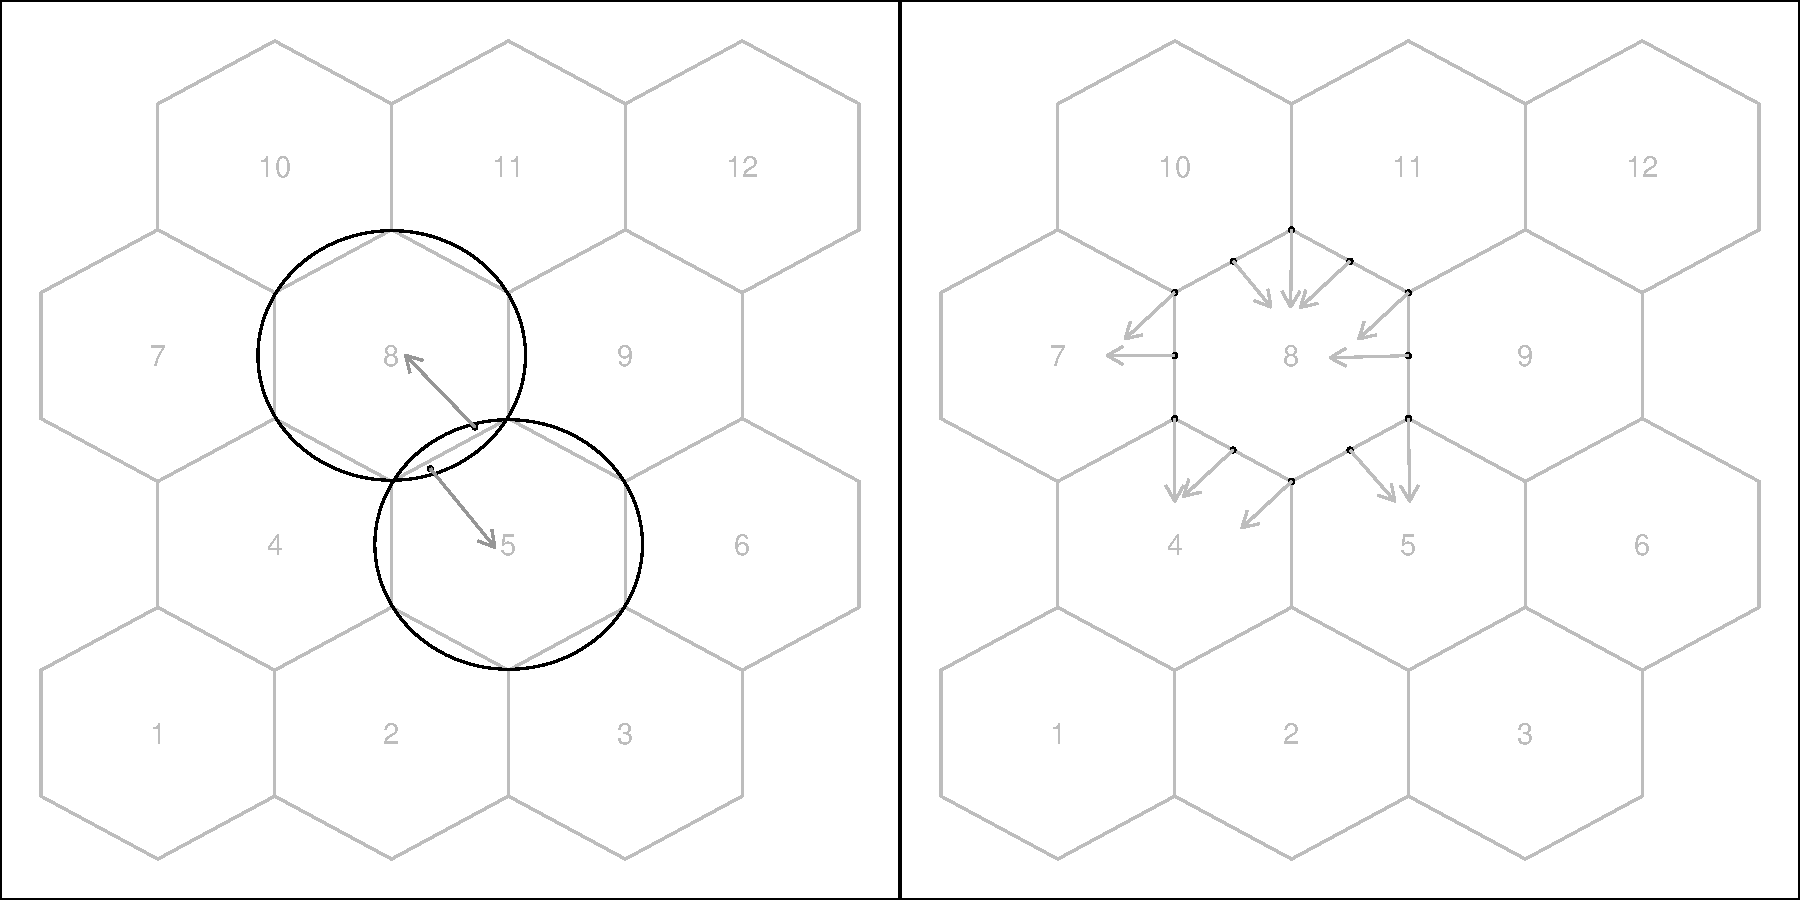
\includegraphics[width=1\linewidth,height=\textheight,keepaspectratio]{appendix/B-appB_files/figure-pdf/fig-assign-data-1.pdf}

}

\caption{\label{fig-assign-data}Binning the data. Points are assigned to
the nearest centroid. If a point is equidistant from multiple centroids,
assigned to the centroid with the smallest bin ID.}

\end{figure}%

\section{Area of a hexagon}\label{area-of-a-hexagon}

The area of a hexagon is defined as \(A = 3\sqrt{3}l^2/2\), where \(l\)
is the side length of the hexagon. \(l\) can be computed using \(a_1\)
and \(a_2\).

\begin{figure}[H]

\centering{

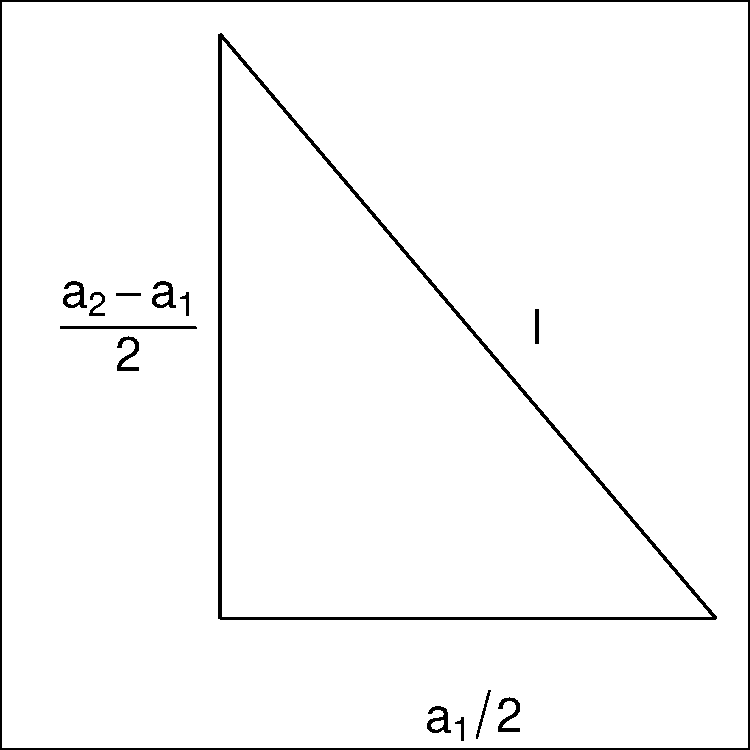
\includegraphics[width=0.3\linewidth,height=\textheight,keepaspectratio]{appendix/B-appB_files/figure-pdf/fig-tri-param-1.pdf}

}

\caption{\label{fig-tri-param}The components of the right triangle
illustrating notation.}

\end{figure}%

By applying the Pythagorean theorem, we obtain,

\[
l^2 = \left(\frac{a_1}{2}\right)^2 + \left(\frac{a_2 - l}{2}\right)^2.
\] Next, rearranging the terms, we get,

\[
l^2 - \left(\frac{a_2 - l}{2}\right)^2 = \left(\frac{a_1}{2}\right)^2,
\]

\[
\left[l - \left(\frac{a_2 - l}{2}\right)\right]\left[l + \left(\frac{a_2 - l}{2}\right)\right] = \left(\frac{a_1}{2}\right)^2,
\]

\[
3l^2 + 2a_2l - (a_1^2 + a_2^2) = 0.
\]

Finally, by solving the quadratic equation, we compute,

\[
l = \frac{-2a_2 \pm \sqrt{4a_2^2 - 24[-(a_1^2 + a_2^2)]}}{6},
\]

\[
l = \frac{-a_2 \pm \sqrt{a_2^2 - 6[-(a_1^2 + a_2^2)]}}{3},
\]

where \(l > 0\).

\section{Curiosities about NLDR results discovered by examining the
model in the data space}\label{sec-curiosities}

With the drawing of the model in the data, several interesting
differences between NLDR methods can be observed.

\subsection{Some methods appear to order points in the
layout}\label{some-methods-appear-to-order-points-in-the-layout}

The \gD{} model representations generated from some NLDR methods,
especially PaCMAP, are unreasonably flat or like a pancake. A simple
example of this can be seen with data simulated to contain five \fD{}
Gaussian clusters. Each cluster is essentially a ball in \fD{}, so there
is no \gD{} representation, rather the model in each cluster should
resemble a crumpled sheet of paper that fills out \fD{}.

Figure~\ref{fig-five-gau-projs} a1, b1, c1 show the \gD{} layouts for
(a) tSNE, (b) UMAP, and (c) PaCMAP, respectively. The default
hyper-parameters for each method are used. In each layout we can see an
accurate representation where all five clusters are visible, although
with varying degrees of separation.

The models are fitted to each these layouts.
Figure~\ref{fig-five-gau-projs} a2, b2, c2 show the fitted models in a
projection of the \fD{} space, taken from a tour. These clusters are
fully \fD{} in nature, so we would expect the model to be a
\emph{crumpled sheet} that stretches in all four dimensions. This is
what is mostly observed for tSNE and UMAP. The curious detail is that
the model for PaCMAP is closer to a \emph{pancake} in shape in every
cluster! This single projection only shows this in three of the five
clusters but if we examine a different projection the other clusters
exhibit the pancake also. While we don't know what exactly causes this,
it is likely due to some ordering of points in the \gD{} PaCMAP layout
that induces the flat model. One could imagine that if the method used
principal components on all the data, that it might induce some ordering
that would produce the flat model. If this were the reason, the
pancaking would be the same in all clusters, but it is not: The pancake
is visible in some clusters in some projections but in other clusters it
is visible in different projections. It might be due to some ordering by
nearest neighbors in a cluster. The PaCMAP documentation doesn't provide
any helpful clues. That this happens, though, makes the PaCMAP layout
inadequate for representing the high-dimensional data.

\begin{figure}[H]

\centering{

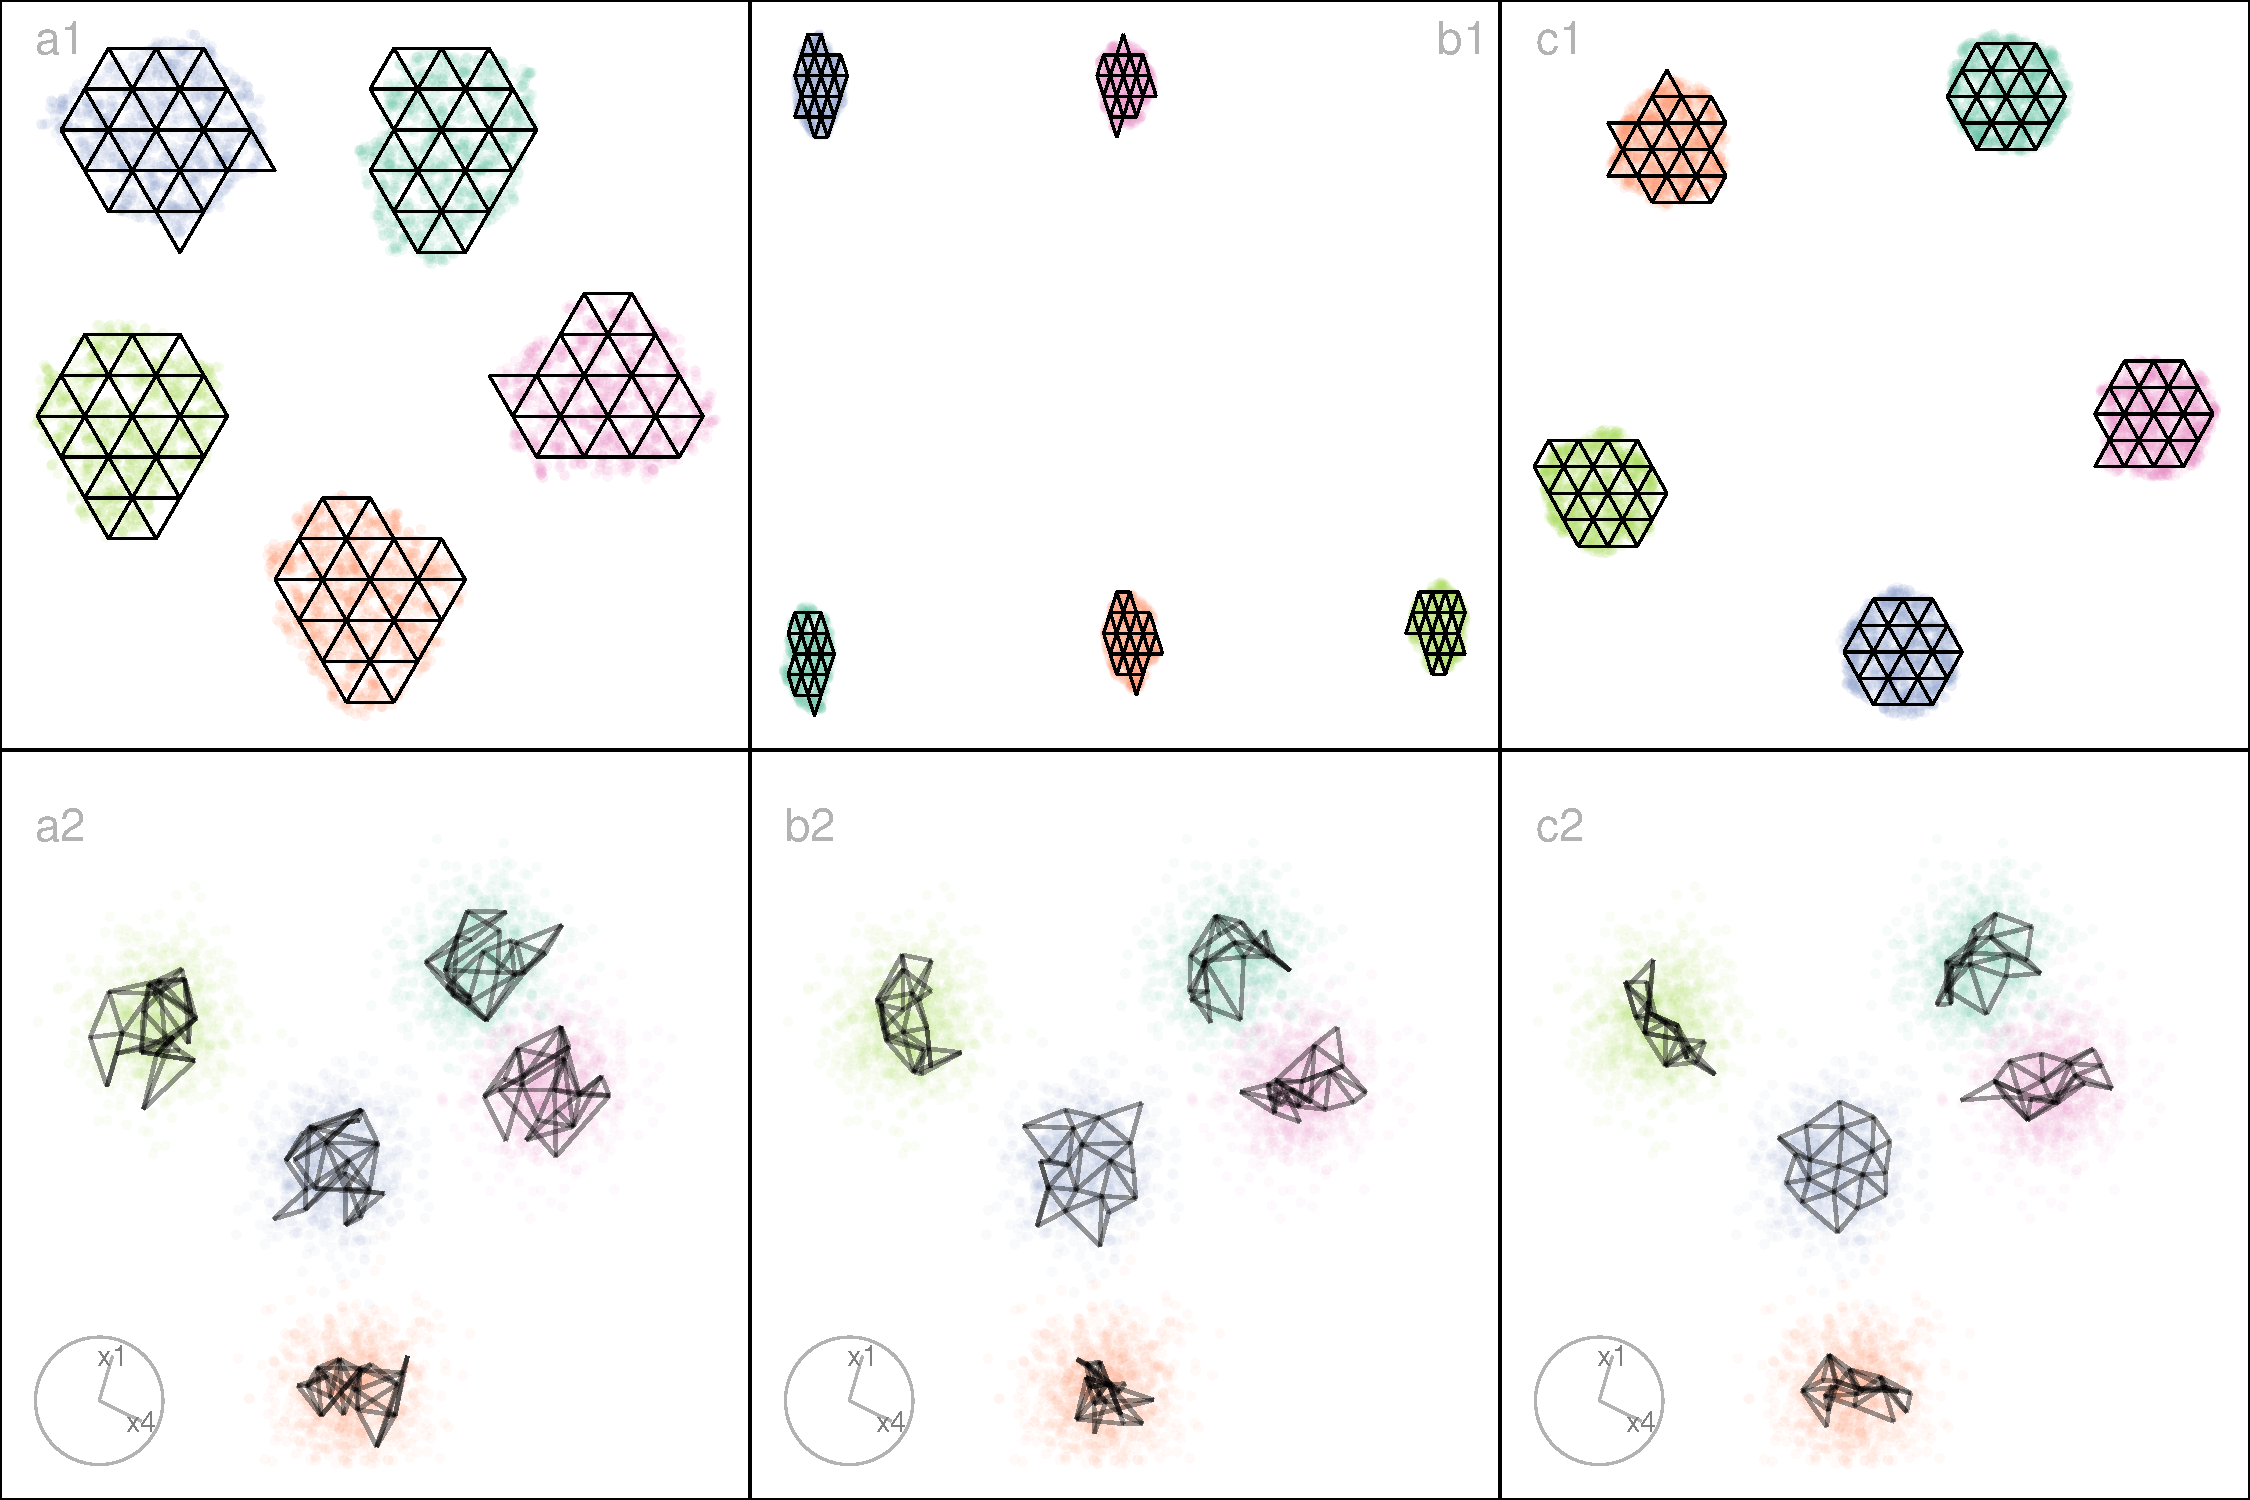
\includegraphics[width=1\linewidth,height=\textheight,keepaspectratio]{appendix/B-appB_files/figure-pdf/fig-five-gau-projs-1.pdf}

}

\caption{\label{fig-five-gau-projs}NLDR's organise points in the \gD{}
layout in different ways, possibly misleadingly, illustrated using three
layouts: (a) tSNE, (b) UMAP, (c) PaCMAP. The data has five Gaussian
clusters in \fD{}. The bottom row of plots shows a \gD{} projection from
a tour on \fD{} revealing the differences generated by the layouts on
the model fits. We would expect the model fit to be like that in (a2)
where it is distinctly is separate for each cluster but like a hairball
in each. This would indicate the distinct clusters, each being fully
\fD{}. With (c2), the curiousity is that the model is a \gD{} pancake
shape in \fD{}, indicating that there is some ordering of points done by
PaCMAP, posisbly along some principal component axes. Videos of the
langevitour animations are available at
\url{https://youtu.be/I-kxCwVfqiQ}, \url{https://youtu.be/gD1P01FUPyU},
and \url{https://youtu.be/MxJ_srOFQNk} respectively.}

\end{figure}%

\subsection{\texorpdfstring{Sparseness creates a contracted \gD{}
layout}{Sparseness creates a contracted  layout}}\label{sec-effect-dens}

Differences in density can arise by sampling at different rates in
different subspaces of \pD{}. For example, the data shown in
Figure~\ref{fig-one-dens_clust-error} all lies on a \gD{} curved sheet
in \fD{}, but one end of the sheet is sampled densely and the other very
sparsely. It was simulated to illustrate the effect of the density
difference on layout generated by an NLDR, illustrated using the tSNE
results, but it happens with all methods.

Figure~\ref{fig-one-dens_clust-error} (a2, b2) shows a \gD{} layout for
tSNE created using the default hyper-parameters. One would expect to see
a rectangular shape if the curved sheet is flattened, but the layout is
triangular. The other two displays show the residuals as a dot density
plot (a1, b1), and a \gD{} projection of the data and the model from
\fD{} (a3, b3). Using linked brushing between the plots, we can
highlight points in the tSNE layout, and examine where they fall in the
original \fD{}. The darker (maroon) points indicate points that have
been highlighted by linking. In row a, the points at the top of the
triangle are highlighted, and we can see these correspond to higher
residuals, and also to all points at the low density end of the curved
sheet. In row b, points at the lower left side of the triangle are
highlighted which corresponds to smaller residuals and one corner of the
sheet at the high density end of the curved sheet.

The tSNE behaviour is to squeeze the low density area of the data
together into the layout. This is common in other NLDR methods also,
which means analysts need to be aware that if their data is not sampled
relatively uniformly, apparent closeness in the \gD{} may correspond to
sparseness in \pD{}.

\begin{figure}[H]

\centering{

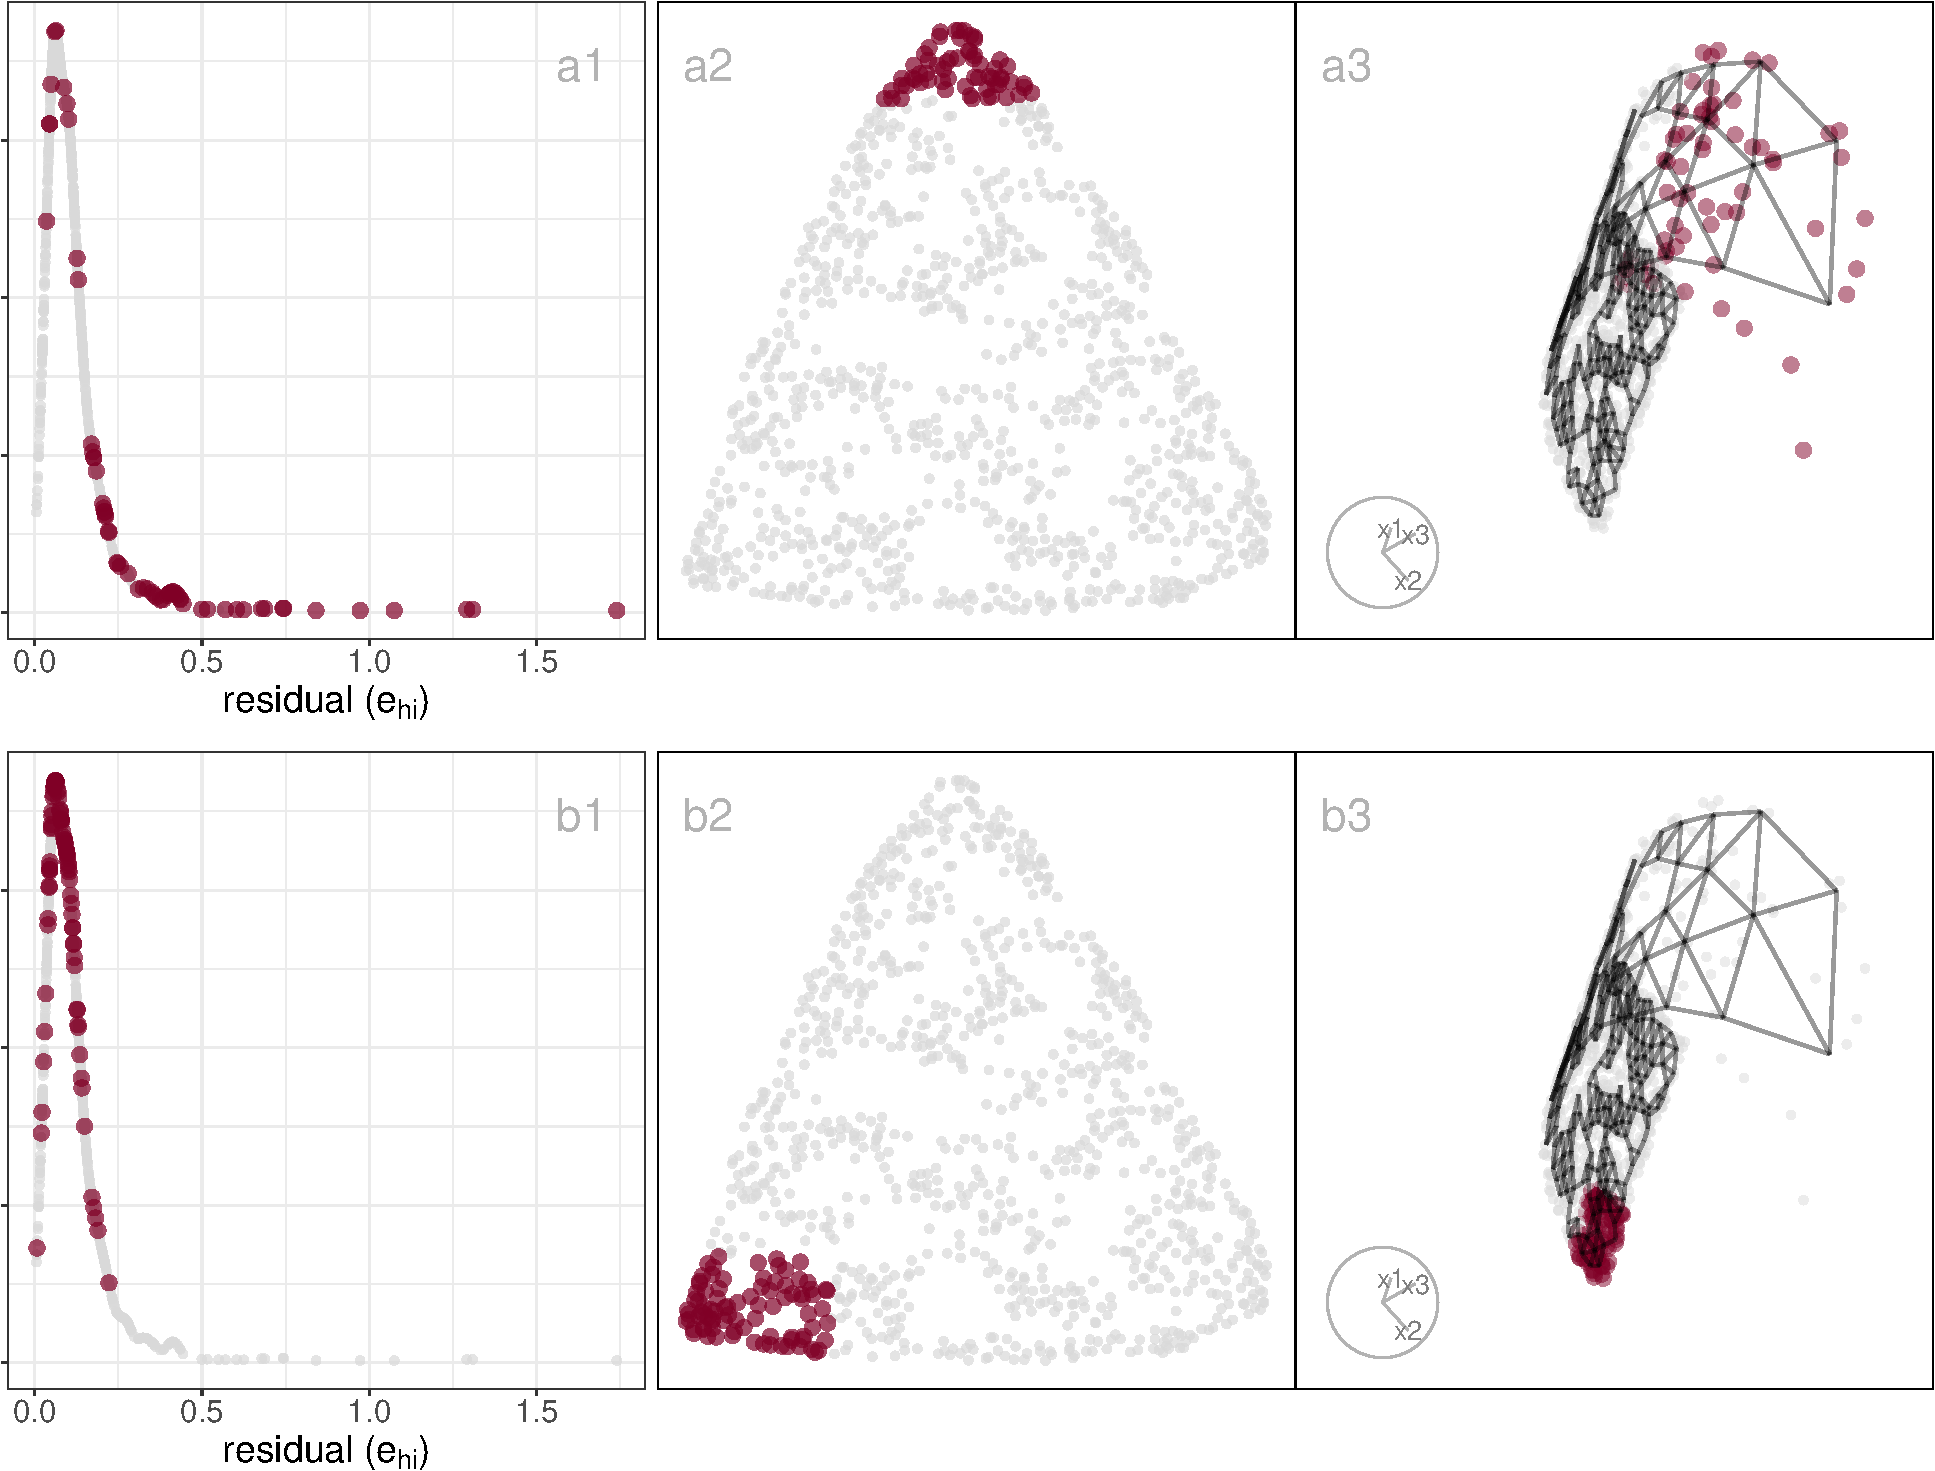
\includegraphics[width=1\linewidth,height=\textheight,keepaspectratio]{appendix/B-appB_files/figure-pdf/fig-one-dens_clust-error-1.pdf}

}

\caption{\label{fig-one-dens_clust-error}Exploring the effect of density
on the NLDR layout using a \gD{} curved sheet in \fD{} with different
density at each end. Three plots are linked: density plot of residuals
(a1, b1), NLDR layout (a2, b2), projection of \fD{} model and data (a3,
b3). The brown points indicate the selected set, which are different in
each row. In (a2), the top part of the triangular shape is selected
which corresponds to higher residuals (a1) and the sparse end of the
structure (a3). In (b2) one of other corners is highlighted, which can
be seen to correspond to low residuals (b1) and one side of the dense
end of the data (b3). While the tSNE layout represents the dense end of
the sheet correctly as two corners in the layout, it contracts the
sparse end of the sheet into a single corner. Video of the langevitour
animation is available at \url{https://youtu.be/-KsQH0rII2A}.}

\end{figure}%

\section{PBMC3k: comparison with results of scDEED
recommendations}\label{pbmc3k-comparison-with-results-of-scdeed-recommendations}

As we were writing this paper Xia et al. (\citeproc{ref-xia2023}{2023})
appeared proposing a new method called scDEED helping to assess the
validity of a \gD{} embedding. scDEED calculates a reliability score for
each cell embedding based on the similarity between the cell's \gD{}
embedding neighbors and its neighbors prior to embedding. A low
reliability score suggests a dubious embedding. It can help in the
deciding on optimal hyper-parameters. Here we illustrate how our method
compares with the results from scDEED.

Note that Xia et al. (\citeproc{ref-xia2023}{2023}) uses a different
PBMC dataset than that used by Chen et al.
(\citeproc{ref-chen2024}{2024}), shown by us in the main paper example,
which is why this comparison is shown here and not in the main paper.
Their data contains \(31,021\) cells including cell type labels, and the
gene expression levels were in the unit of log-transformed UMI count per
\(10,000\). They focused on three sequencing methods (inDrops, DropSeq,
and SeqWell) and four common cell types Cytotoxic T cell, CD4+T cell,
CD14+ Monocyte, and B cell. Pre-processing follows the process in Xia et
al. (\citeproc{ref-xia2023}{2023}) again using the Human Peripheral
Blood Mononuclear Cells (PBMC) data.

For illustration purposes, we only selected cells generated with inDrops
(\(n=5858\) cells). Also, Xia et al. (\citeproc{ref-xia2023}{2023}) used
first \(9\) principal components to generate the UMAP and tSNE with
default hyper-parameters. The objective is to what scDEED suggests is
the best layout with what HBE would choose. Layout a
(Figure~\ref{fig-pbmc-mse-umap}) is generated from the hyper-parameters
suggested by Chen et al. (\citeproc{ref-chen2024}{2024}), and layout b
(Figure~\ref{fig-pbmc-mse-umap}) is with suggested hyper-parameters by
scDEED to be more accurate. The HBE vs binwidth (\(a_1\)) plot
(Figure~\ref{fig-pbmc-mse-umap}) illustrates that our approach would
suggest that scDEED is correct here, that layout b is more accurately
reflecting the cluster structure in the PBMC data. This is also
supported by examining the models in the data space as shown in
Figure~\ref{fig-model-pbmc-author-proj}.

Figure~\ref{fig-pbmc-mse-umap} compares the metrics ARNX, RTA, SC, GS,
along with HBE computed on \(a_1=0.04\) for the six layouts shown in
Figure~\ref{fig-pbmc-mse-umap}. This is a parallel coordinate plot where
the y-axis shows a normalized score to ensure the metrics are on the
same scale. Each line corresponds to one layout. The metric ARNX has
been reversed so that it aligns with HBE - the lower the value the
better the layout. Most metrics (ARNX, RTA, GS, and HBE) consistently
indicate that the optimised layout (b) provides a better representation,
while SC slightly favors the published layout.

\begin{figure}[H]

\centering{

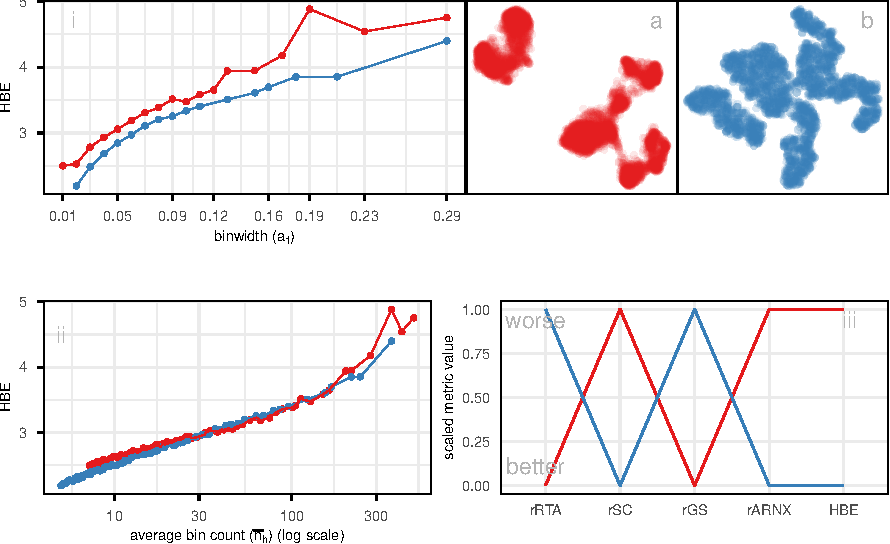
\includegraphics[width=1\linewidth,height=\textheight,keepaspectratio]{appendix/B-appB_files/figure-pdf/fig-pbmc-mse-umap-1.pdf}

}

\caption{\label{fig-pbmc-mse-umap}Comparing the published layout (a)
with what would be suggested to be optimal by scDEED (b), using HBE vs
\(a_1\), on a subset of PBMC3k data. Color represents NLDR layouts. HBE
would corroborate that the scDEED optimised layout is better than what
was originally published. Comparison of scaled evaluation metrics (rRTA,
rSC, rGS, rARNX, and HBE using \(a_1=0.04\)) for two NLDR layouts of the
PBMC3k data the originally published layout (a) and the scDEED optimised
layout (b). Each line represents a layout, with color matching the
corresponding scatterplots. Most metrics (rSC, rARNX, and HBE)
consistently indicate that the optimised layout (b) provides a better
representation, while rRTA, and rGS slightly favor the published
layout.}

\end{figure}%

\begin{figure}[H]

\centering{

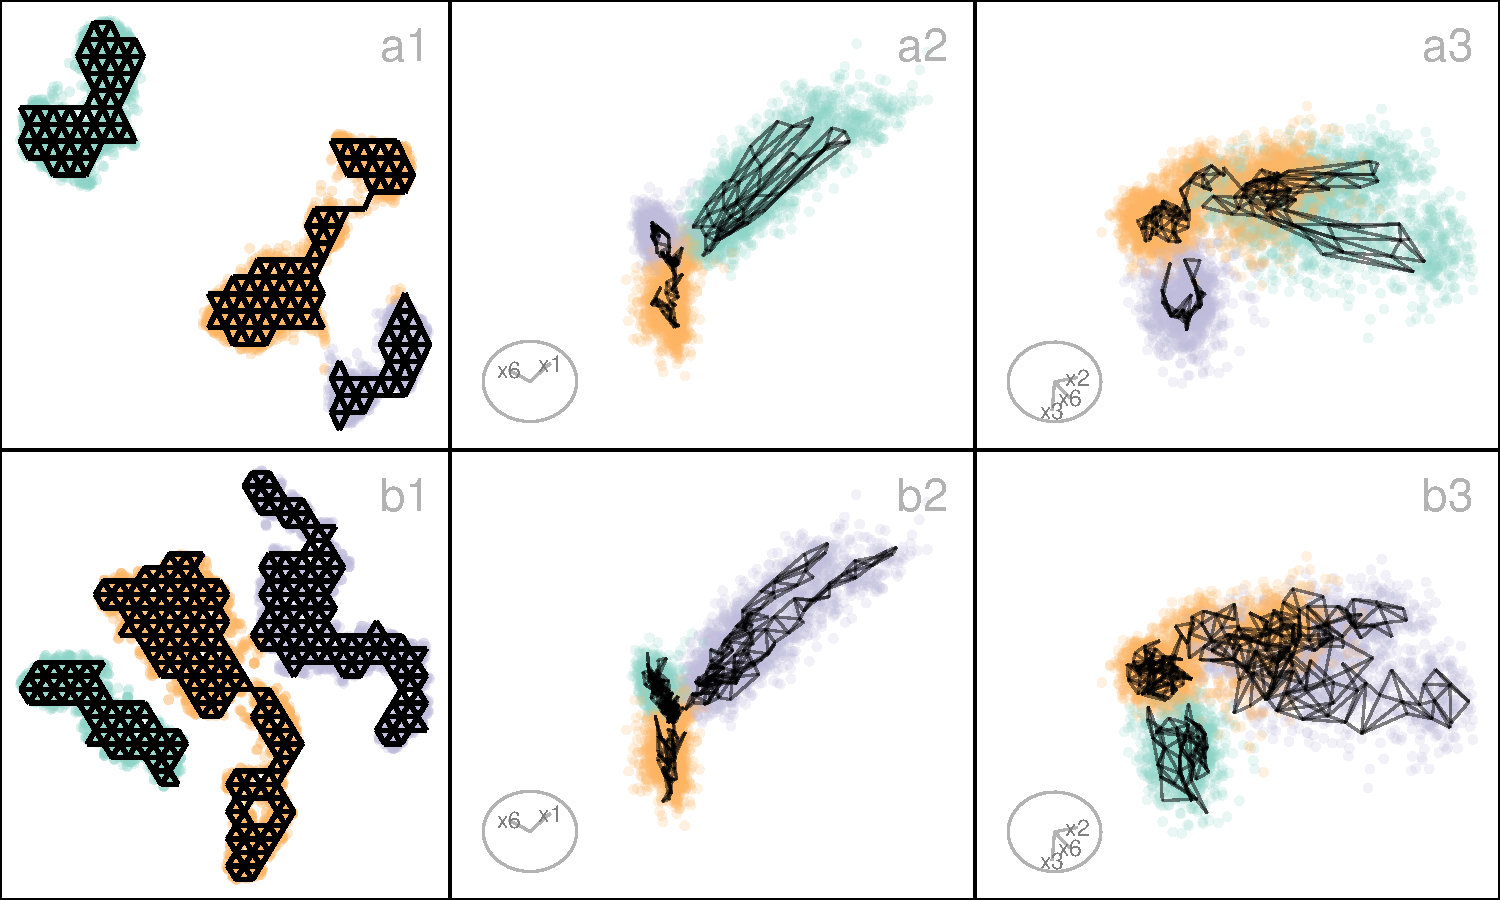
\includegraphics[width=0.9\linewidth,height=\textheight,keepaspectratio]{appendix/B-appB_files/figure-pdf/fig-model-pbmc-author-proj-1.pdf}

}

\caption{\label{fig-model-pbmc-author-proj}Compare the published \gD{}
layout (Figure~\ref{fig-pbmc-mse-umap} a) made with UMAP and the \gD{}
layout made with tSNE selected as optimal by scDEED and also HBE
(Figure~\ref{fig-pbmc-mse-umap} b)(Figure~\ref{fig-pbmc-mse-umap}). The
two plots on the right show projections from a tour, with the models
overlaid. The published layout a suggested three separated clusters with
two of them are close, but this is not present in the data. While there
may be three clusters they are not well-separated. The difference in
model fit also indicates this: the published layout a does not capture
the nonlinear structure of the clusters like the model generated from
layout b. This supports the choice that layout b is the better
representation of the data, because it shows close clusters. Videos of
the langevitour animations are available at
\url{https://youtu.be/ffiB4MGWyn8} and
\url{https://youtu.be/e7XNL18co1c} respectively.}

\end{figure}%

\section{Compare HBE with existing evaluation
metrics}\label{compare-hbe-with-existing-evaluation-metrics}

Figure~\ref{fig-comp-metric-pbmc} and Figure~\ref{fig-comp-metric-mnist}
compare HBE with commonly used evaluation metrics such as RTA, ARNX, sc,
and GS across multiple NLDR layouts. These visual comparisons highlight
that HBE behaves differently from these existing metrics due to the
different settings involved.

\begin{figure}[H]

\centering{

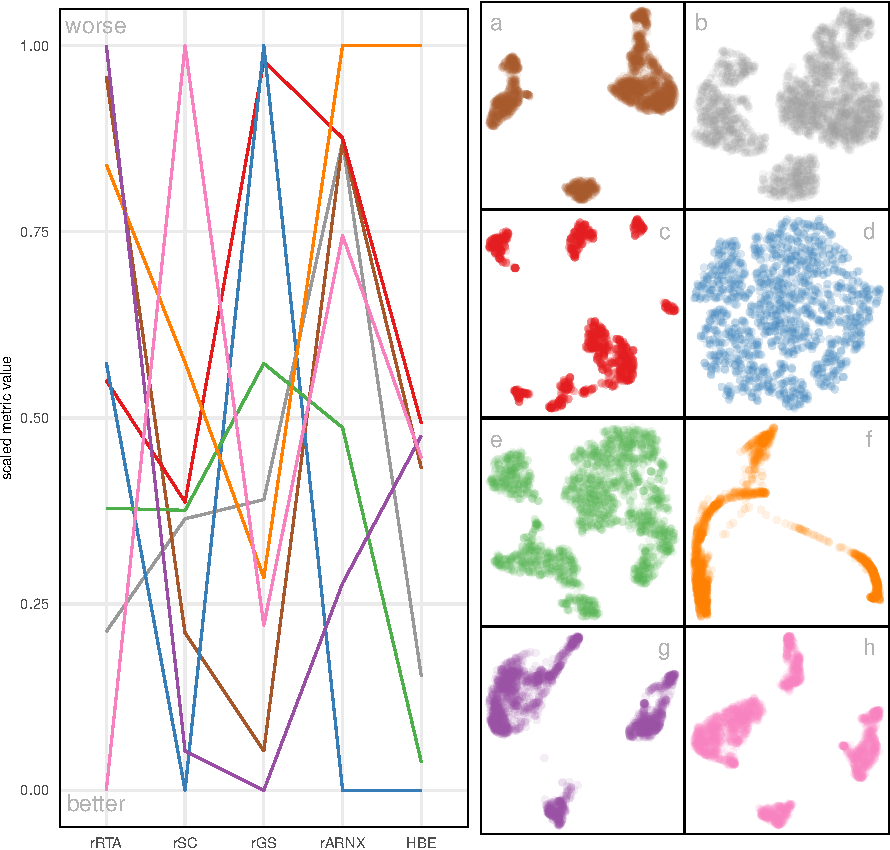
\includegraphics[width=1\linewidth,height=\textheight,keepaspectratio]{appendix/B-appB_files/figure-pdf/fig-comp-metric-pbmc-1.pdf}

}

\caption{\label{fig-comp-metric-pbmc}Comparison of scaled evaluation
metrics (rRTA, rSC, rGS, rARNX, and HBE with \(a_1 = 0.06\)) for the
eight NLDR layouts computed on the PBMC3k data, shown as a parallel
coordinate plot. The color of each line corresponds to an NLDR layout.
RTA, SC, GS, and ARNX is reversed so that lower is best. Overall, the
metrics show general agreement, with minor differences in ranking. All
metrics except SC suggest that layouts d and e outperform layout b.
ARNX, GS, and HBE consistently identify layout d as the best, with
layout e also performing well.}

\end{figure}%

\begin{figure}[H]

\centering{

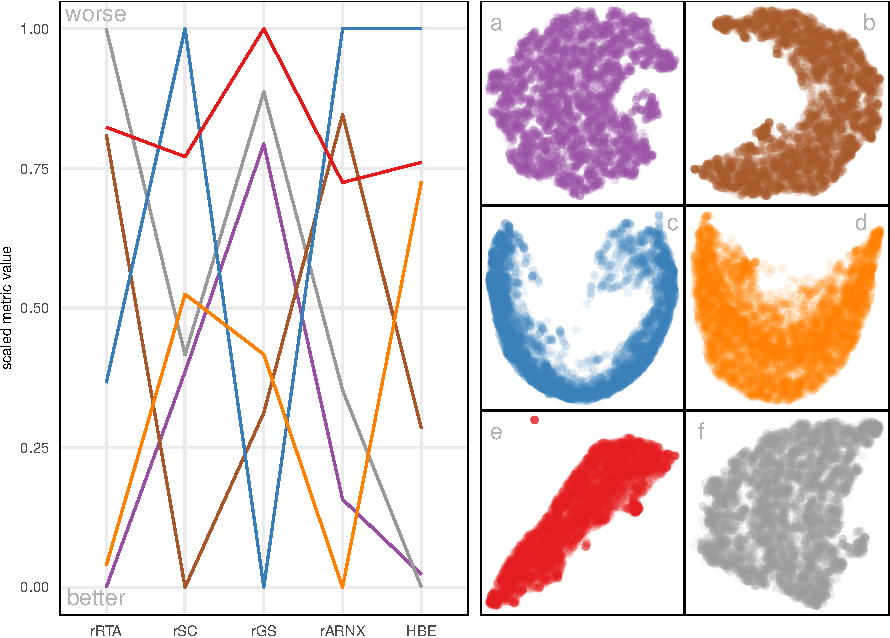
\includegraphics[width=1\linewidth,height=\textheight,keepaspectratio]{appendix/B-appB_files/figure-pdf/fig-comp-metric-mnist-1.pdf}

}

\caption{\label{fig-comp-metric-mnist}Comparison of scaled evaluation
metrics (ARNX, RTA, SC, GS, and HBE using \(a_1=0.04\)) for six NLDR
layouts computed on the MNIST digit 1 data using a parallel coordinate
plot. Each line represents a layout (a--f), with colors corresponding to
the scatterplots shown on the right. The metrics display different
ranking patterns, indicating that no single measure fully captures
embedding quality. ARNX, SC, and GS tend to agree, while RTA and HBE
highlight different aspects of structure preservation. Layout c is
consistently poor across all metrics, while layouts a and f are
generally rated highest except in RTA. Interestingly, ARNX and GS
identify layout a as best, whereas HBE and RTA prefer layout f.}

\end{figure}%

\chapter{Appendix to ``Perception and Misperception in Nonlinear
Dimension Reduction: A User Study''}\label{sec-appendix-b}

\section{Videos links}\label{videos-links-1}

Animations of the \pD{} tours that used for the study are available on
YouTube at the links given in Table~\ref{tbl-links-html}.

\begin{longtable}[]{@{}llll@{}}

\caption{\label{tbl-links-html}Videos}

\tabularnewline

\toprule\noalign{}
data structure & small & medium & large \\
\midrule\noalign{}
\endhead
\bottomrule\noalign{}
\endlastfoot
three\_clust\_01 &
\href{https://youtu.be/kZyZxujDz58}{youtu.be/kZyZxujDz58} &
\href{https://youtu.be/Jz3k4uIAiRo}{youtu.be/Jz3k4uIAiRo} &
\href{https://youtu.be/E9msE_XX0KA}{youtu.be/E9msE\_XX0KA} \\
three\_clust\_02 &
\href{https://youtu.be/CLMlOU4Fb2w}{youtu.be/CLMlOU4Fb2w} &
\href{https://youtu.be/TFj0satlBBE}{youtu.be/TFj0satlBBE} &
\href{https://youtu.be/_f2WvtD2xog}{youtu.be/f2WvtD2xog} \\
three\_clust\_03 &
\href{https://youtu.be/K2oKM4mUBXM}{youtu.be/K2oKM4mUBXM} &
\href{https://youtu.be/b-43HKN30ws}{youtu.be/b-43HKN30ws} &
\href{https://youtu.be/7NwNcD4qlLc}{youtu.be/7NwNcD4qlLc} \\
three\_clust\_04 &
\href{https://youtu.be/7yvvpPgiWNw}{youtu.be/7yvvpPgiWNw} &
\href{https://youtu.be/1PhZO7cUEaI}{youtu.be/1PhZO7cUEaI} &
\href{https://youtu.be/XO61YVXAdr8}{youtu.be/XO61YVXAdr8} \\
three\_clust\_05 &
\href{https://youtu.be/pbI7UXFgc0k}{youtu.be/pbI7UXFgc0k} &
\href{https://youtu.be/G-TvOIBj-14}{youtu.be/G-TvOIBj-14} &
\href{https://youtu.be/ardE0G7zevk}{youtu.be/ardE0G7zevk} \\
three\_clust\_06 &
\href{https://youtu.be/Mxylk4M67iA}{youtu.be/Mxylk4M67iA} &
\href{https://youtu.be/ABrxozu8F-A}{youtu.be/ABrxozu8F-A} &
\href{https://youtu.be/soFQR9UwNsg}{youtu.be/soFQR9UwNsg} \\
three\_clust\_07 &
\href{https://youtu.be/2a89BQGK_iU}{youtu.be/2a89BQGK\_iU} &
\href{https://youtu.be/Wt4NwZSACmo}{youtu.be/Wt4NwZSACmo} &
\href{https://youtu.be/hVwIjSxACoo}{youtu.be/hVwIjSxACoo} \\
three\_clust\_08 &
\href{https://youtu.be/eID-dwpgU44}{youtu.be/eID-dwpgU44} &
\href{https://youtu.be/ILwnlZUMj_U}{youtu.be/ILwnlZUMj\_U} &
\href{https://youtu.be/oSBaMH9HJZ4}{youtu.be/oSBaMH9HJZ4} \\
three\_clust\_09 &
\href{https://youtu.be/6uGCDUSL60Q}{youtu.be/6uGCDUSL60Q} &
\href{https://youtu.be/RvlSY3drV5I}{youtu.be/RvlSY3drV5I} &
\href{https://youtu.be/mh_rG2qy2Pc}{youtu.be/mh\_rG2qy2Pc} \\
three\_clust\_10 &
\href{https://youtu.be/CX5O4eNZW5o}{youtu.be/CX5O4eNZW5o} &
\href{https://youtu.be/fHxflXa9i-s}{youtu.be/fHxflXa9i-s} &
\href{https://youtu.be/R6vD1xJH21w}{youtu.be/R6vD1xJH21w} \\
three\_clust\_11 &
\href{https://youtu.be/1f8S7HiZ8dc}{youtu.be/1f8S7HiZ8dc} &
\href{https://youtu.be/Fki5vIuPupE}{youtu.be/Fki5vIuPupE} &
\href{https://youtu.be/ciVOD8_sWR0}{youtu.be/ciVOD8\_sWR0} \\
three\_clust\_12 &
\href{https://youtu.be/AZv45NGkuC4}{youtu.be/AZv45NGkuC4} &
\href{https://youtu.be/qQ4LqHYH_c4}{youtu.be/qQ4LqHYH\_c4} &
\href{https://youtu.be/Y2sfVoemVZo}{youtu.be/Y2sfVoemVZo} \\
three\_clust\_13 &
\href{https://youtu.be/U-bbZjzvaiE}{youtu.be/U-bbZjzvaiE} &
\href{https://youtu.be/0MznMYr5gfo}{youtu.be/0MznMYr5gfo} &
\href{https://youtu.be/E7ge3kw5Q0Q}{youtu.be/E7ge3kw5Q0Q} \\
three\_clust\_14 &
\href{https://youtu.be/ynu2oUxv08I}{youtu.be/ynu2oUxv08I} &
\href{https://youtu.be/gHDLMn5AG-8}{youtu.be/gHDLMn5AG-8} &
\href{https://youtu.be/HyCJEiwCVv0}{youtu.be/HyCJEiwCVv0} \\
three\_clust\_15 &
\href{https://youtu.be/xsdWsBek0eQ}{youtu.be/xsdWsBek0eQ} &
\href{https://youtu.be/SDY64MrcWQg}{youtu.be/SDY64MrcWQg} &
\href{https://youtu.be/CFIyW7ftF9M}{youtu.be/CFIyW7ftF9M} \\
three\_clust\_16 &
\href{https://youtu.be/VyYyYOqhOVs}{youtu.be/VyYyYOqhOVs} &
\href{https://youtu.be/zi-TvgVR8a4}{youtu.be/zi-TvgVR8a4} &
\href{https://youtu.be/hdQmD499yo8}{youtu.be/hdQmD499yo8} \\
three\_clust\_17 &
\href{https://youtu.be/yojgjcf2NQk}{youtu.be/yojgjcf2NQk} &
\href{https://youtu.be/UJPMJ5irRbQ}{youtu.be/UJPMJ5irRbQ} &
\href{https://youtu.be/zdQYQvqTyGA}{youtu.be/zdQYQvqTyGA} \\
three\_clust\_18 &
\href{https://youtu.be/r-Z1Yyf2c4s}{youtu.be/r-Z1Yyf2c4s} &
\href{https://youtu.be/2Rf2L8iey2w}{youtu.be/2Rf2L8iey2w} &
\href{https://youtu.be/e_-IQycglVE}{youtu.be/e\_-IQycglVE} \\

\end{longtable}

\section{Scripts}\label{scripts-1}

\section{Generating non-attention check data
structures}\label{generating-non-attention-check-data-structures}

Excellent --- this section can be turned into a smooth, cohesive
narrative that reads like an appendix entry in a methodological paper,
where each data-generating function is described mathematically
\emph{and} conceptually. Here's a refined version written in a unified
academic style with mathematical explanations integrated naturally into
the prose.

\section{\texorpdfstring{\gD{} layouts}{ layouts}}\label{layouts}

All \gD{} layouts used in the experiment are available in the
supplementary repository:
\href{https://github.com/JayaniLakshika/paper-vis-experiment/tree/main/figures/layouts}{github.com/JayaniLakshika/paper-vis-experiment/tree/main/figures/layouts}.
These include all \gD{} embeddings generated under different NLDR
methods with default hyper-parameter settings for the simulated
high-dimensional data structures.

\section{Distance metrics}\label{distance-metrics}

To evaluate how well NLDR methods preserve the underlying structure of
high-dimensional data, we considered several inter-cluster distance
metrics that quantify the degree of cluster separation. These metrics
provide complementary perspectives on how distinct or overlapping
clusters are in the original space, allowing quantitative comparison of
separability across NLDR methods.

\begin{figure}

\centering{

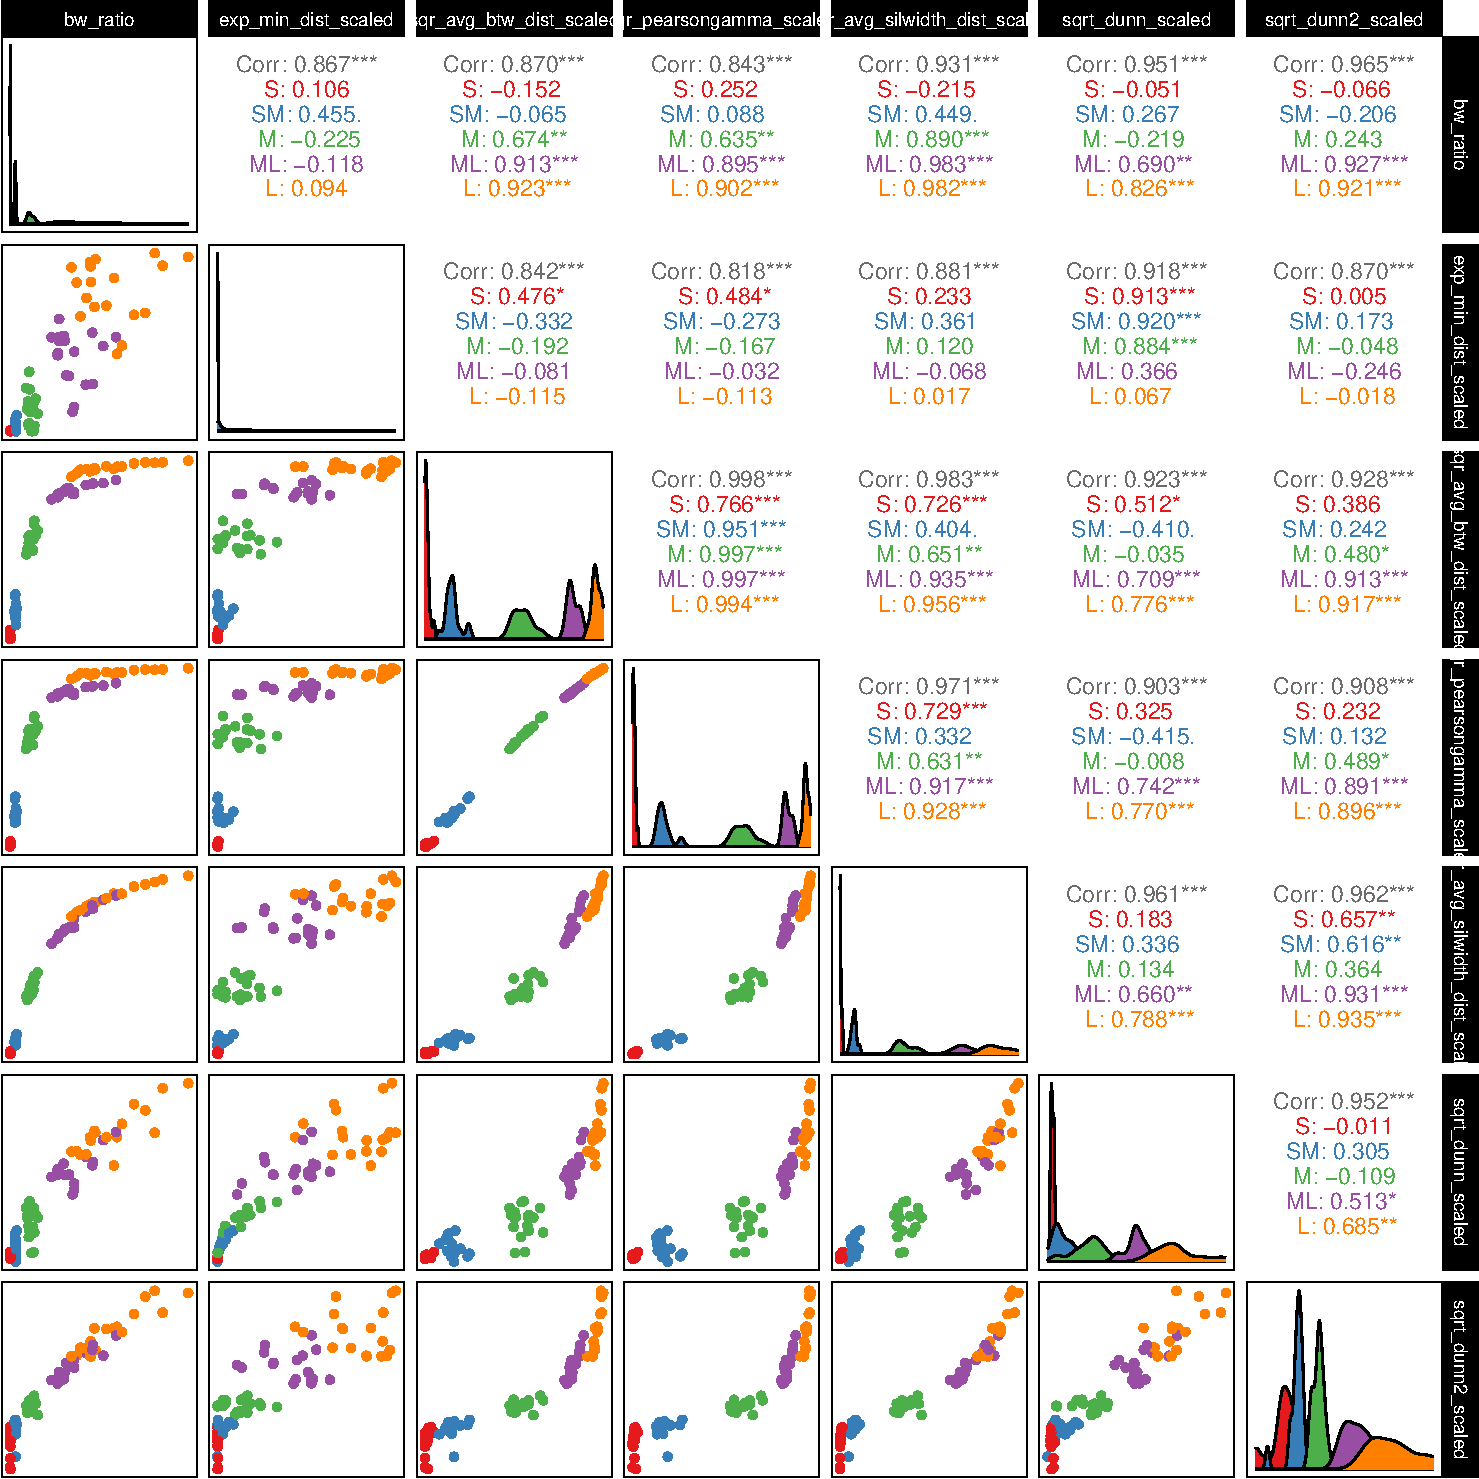
\includegraphics[width=1\linewidth,height=\textheight,keepaspectratio]{appendix/C-appC_files/figure-pdf/fig-distance-metrics-1.pdf}

}

\caption{\label{fig-distance-metrics}Pairwise relationships among six
distance metrics used to quantify cluster separation in the
high-dimensional space: between--within (BW) ratio, exponentiated scaled
minimum distance, quantile-ranked average between-cluster distance,
Pearson--Gamma coefficient, average silhouette distance, and
square-root--transformed Dunn and Dunn2 indices. The diagonal panels
show the distribution of each metric, while the lower panels depict
scatterplots colored by distance scaling factor (0.1--1.1). Upper panels
report Pearson correlation coefficients for all pairs, with significance
indicated by asterisks (*** p \textless{} 0.001). Metrics show high
positive correlation, confirming that they capture consistent structural
variation. The BW ratio and exponentiated minimum distance were chosen
for the main analysis because they provide complementary summaries of
global cluster separation and local boundary distance, which are
directly interpretable in the context of NLDR evaluation.}

\end{figure}%

We examined six metrics commonly used in clustering validation studies:

\subsection{Between--Within (BW) Ratio}\label{betweenwithin-bw-ratio}

The \textbf{between--within ratio} compares average inter-cluster
distances to average intra-cluster distances: \[
BW = \frac{B}{W},
\] where

\[
B = \frac{1}{K(K-1)} \sum_{i < j} ||\mu_i - \mu_j||,
\quad
W = \frac{1}{K} \sum_{i=1}^{K} \frac{1}{n_i} \sum_{x \in C_i} ||x - \mu_i||,
\]

\(K\) is the number of clusters, \(n_i\) is the size of cluster \(i\),
\(C_i\) denotes the set of points in cluster \(i\), and \(\mu_i\) is its
centroid. A higher (BW) ratio indicates greater global separation
relative to within-cluster compactness.

\subsection{Minimum Distance Between
Clusters}\label{minimum-distance-between-clusters}

The \textbf{minimum distance} identifies the closest approach between
two clusters: \[
d_{\min} = \min_{i \neq j} \min_{x \in C_i, , y \in C_j} ||x - y||.
\] This metric is sensitive to boundary overlap and captures
\textbf{local proximity} between clusters.

\subsection{Average Distance Between
Clusters}\label{average-distance-between-clusters}

The \textbf{average inter-cluster distance} represents the overall
separation across all cluster pairs: \[
d_{\text{avg}} = \frac{1}{K(K-1)} \sum_{i < j} \frac{1}{n_i n_j}
\sum_{x \in C_i} \sum_{y \in C_j} ||x - y||.
\] This provides a smooth measure of global spacing between clusters.

\subsection{Pearson--Gamma Coefficient}\label{pearsongamma-coefficient}

The \textbf{Pearson--Gamma coefficient} measures the correlation between
pairwise distances and binary cluster membership: \[
\Gamma = \text{corr}(D, M),
\] where \(D\) is the vector of pairwise Euclidean distances and \(M\)
is a binary indicator matrix (\(M_{pq} = 1\) if points \(p\) and \(q\)
belong to the same cluster, \(0\) otherwise). A larger \(\Gamma\)
indicates stronger agreement between geometric and categorical
separations.

\subsection{Average Silhouette
Distance}\label{average-silhouette-distance}

The \textbf{silhouette width} for each observation \(x_i\) is defined as
\[
s_i = \frac{b_i - a_i}{\max(a_i, b_i)},
\] where \(a_i\) is the average distance between \(x_i\) and all other
points in its own cluster, and \(b_i\) is the minimum average distance
from \(x_i\) to all other clusters. The \textbf{average silhouette} is
then \[
S = \frac{1}{n} \sum_{i=1}^{n} s_i,
\] indicating how well each point matches its assigned cluster compared
to others.

\subsection{Dunn and Dunn2 Indices}\label{dunn-and-dunn2-indices}

The \textbf{Dunn index} evaluates compactness and separation
simultaneously: \[
D = \frac{\min_{i \neq j} d(C_i, C_j)}{\max_{k} \delta(C_k)},
\] where \(d(C_i, C_j)\) is the inter-cluster distance and
\(\delta(C_k)\) is the within-cluster diameter. The \textbf{Dunn2 index}
is a variation that replaces Euclidean distances with average pairwise
distances within and between clusters for improved robustness.

Because these metrics differ in scale and sensitivity, all were
standardized and, where necessary, transformed to stabilize non-linear
relationships. Specifically, the minimum distance was exponentiated
(\texttt{exp(min\_dist\_scaled)}) to linearize its association with
other metrics and reduce the effect of small distance ranges. This
transformation allows for clearer comparison across metrics that vary in
numerical range or distribution.

The pairwise correlations among all metrics
(Figure~\ref{fig-distance-metrics}) demonstrate strong positive
associations, indicating that they generally capture consistent patterns
of cluster separation. However, the BW ratio and minimum distance were
selected as the primary indicators for subsequent analyses. Together,
they summarize both global separation (centroid-based distance
normalized by cluster spread) and local proximity (the smallest
inter-cluster gap). This combination provides a balanced
characterization of cluster distinctness that is both geometrically
interpretable and perceptually meaningful for visualization studies.

\section{Experimental factors allocation to
participants}\label{experimental-factors-allocation-to-participants}

Allocation of participants to experimental factors is an important part
of experimental design. There are a total of \(3 \times 5 = 15\)
combinations of factors for the study. Thirty-six replications for each
combination results in \(10 \times 36 = 360\) evaluations.

Each factor combination must be evaluated by at least thirty-six
participants. Based on the pilot studies for this experiment, we decided
to record \(20\) evaluations for the study, all conducted within a time
frame of \(5\) to \(10\) minutes. One of the evaluations, featuring
three Gaussian clusters, was used as an attention check to ensure data
quality. Additionally, three of the evaluations were assigned different
data displayed across two displays to reduce the consistency of showing
the same data.

Figure~\ref{fig-validate-exp-design-ds} provides an example of how
distance scale factor is allocated using data structures for the first
nine participants. It can be observed that the factor combinations are
assigned randomly to the data structures among the participants,
ensuring a diverse set of data structures for each individual.

\begin{figure}[H]

\centering{

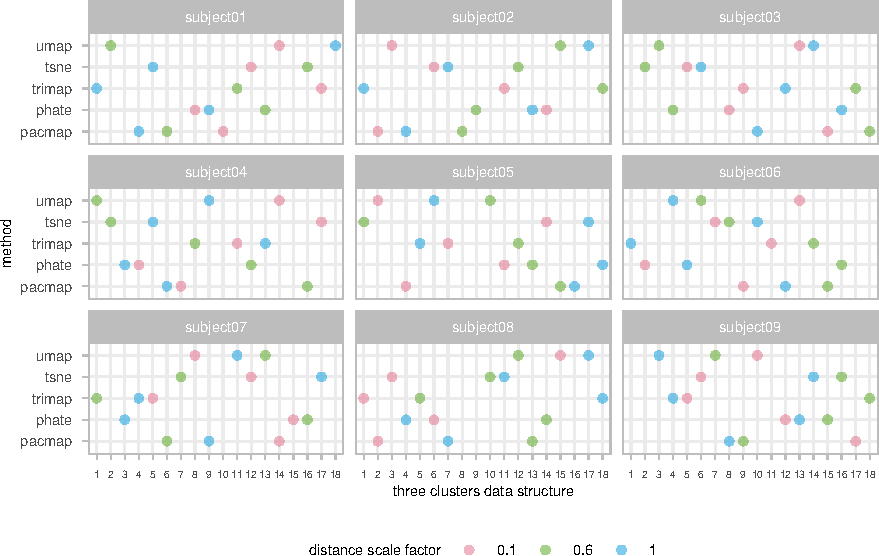
\includegraphics[width=1\linewidth,height=\textheight,keepaspectratio]{appendix/C-appC_files/figure-pdf/fig-validate-exp-design-ds-1.pdf}

}

\caption{\label{fig-validate-exp-design-ds}Allocation of method and
distance scale factor to the first 9 participants for the SAME attempts
only. Each participant has experienced all factor combinations with
randomly assigned data structures.}

\end{figure}%

XXX Add description regarding how experimental factors are allocated to
the subjects

\begin{figure}[H]

\centering{

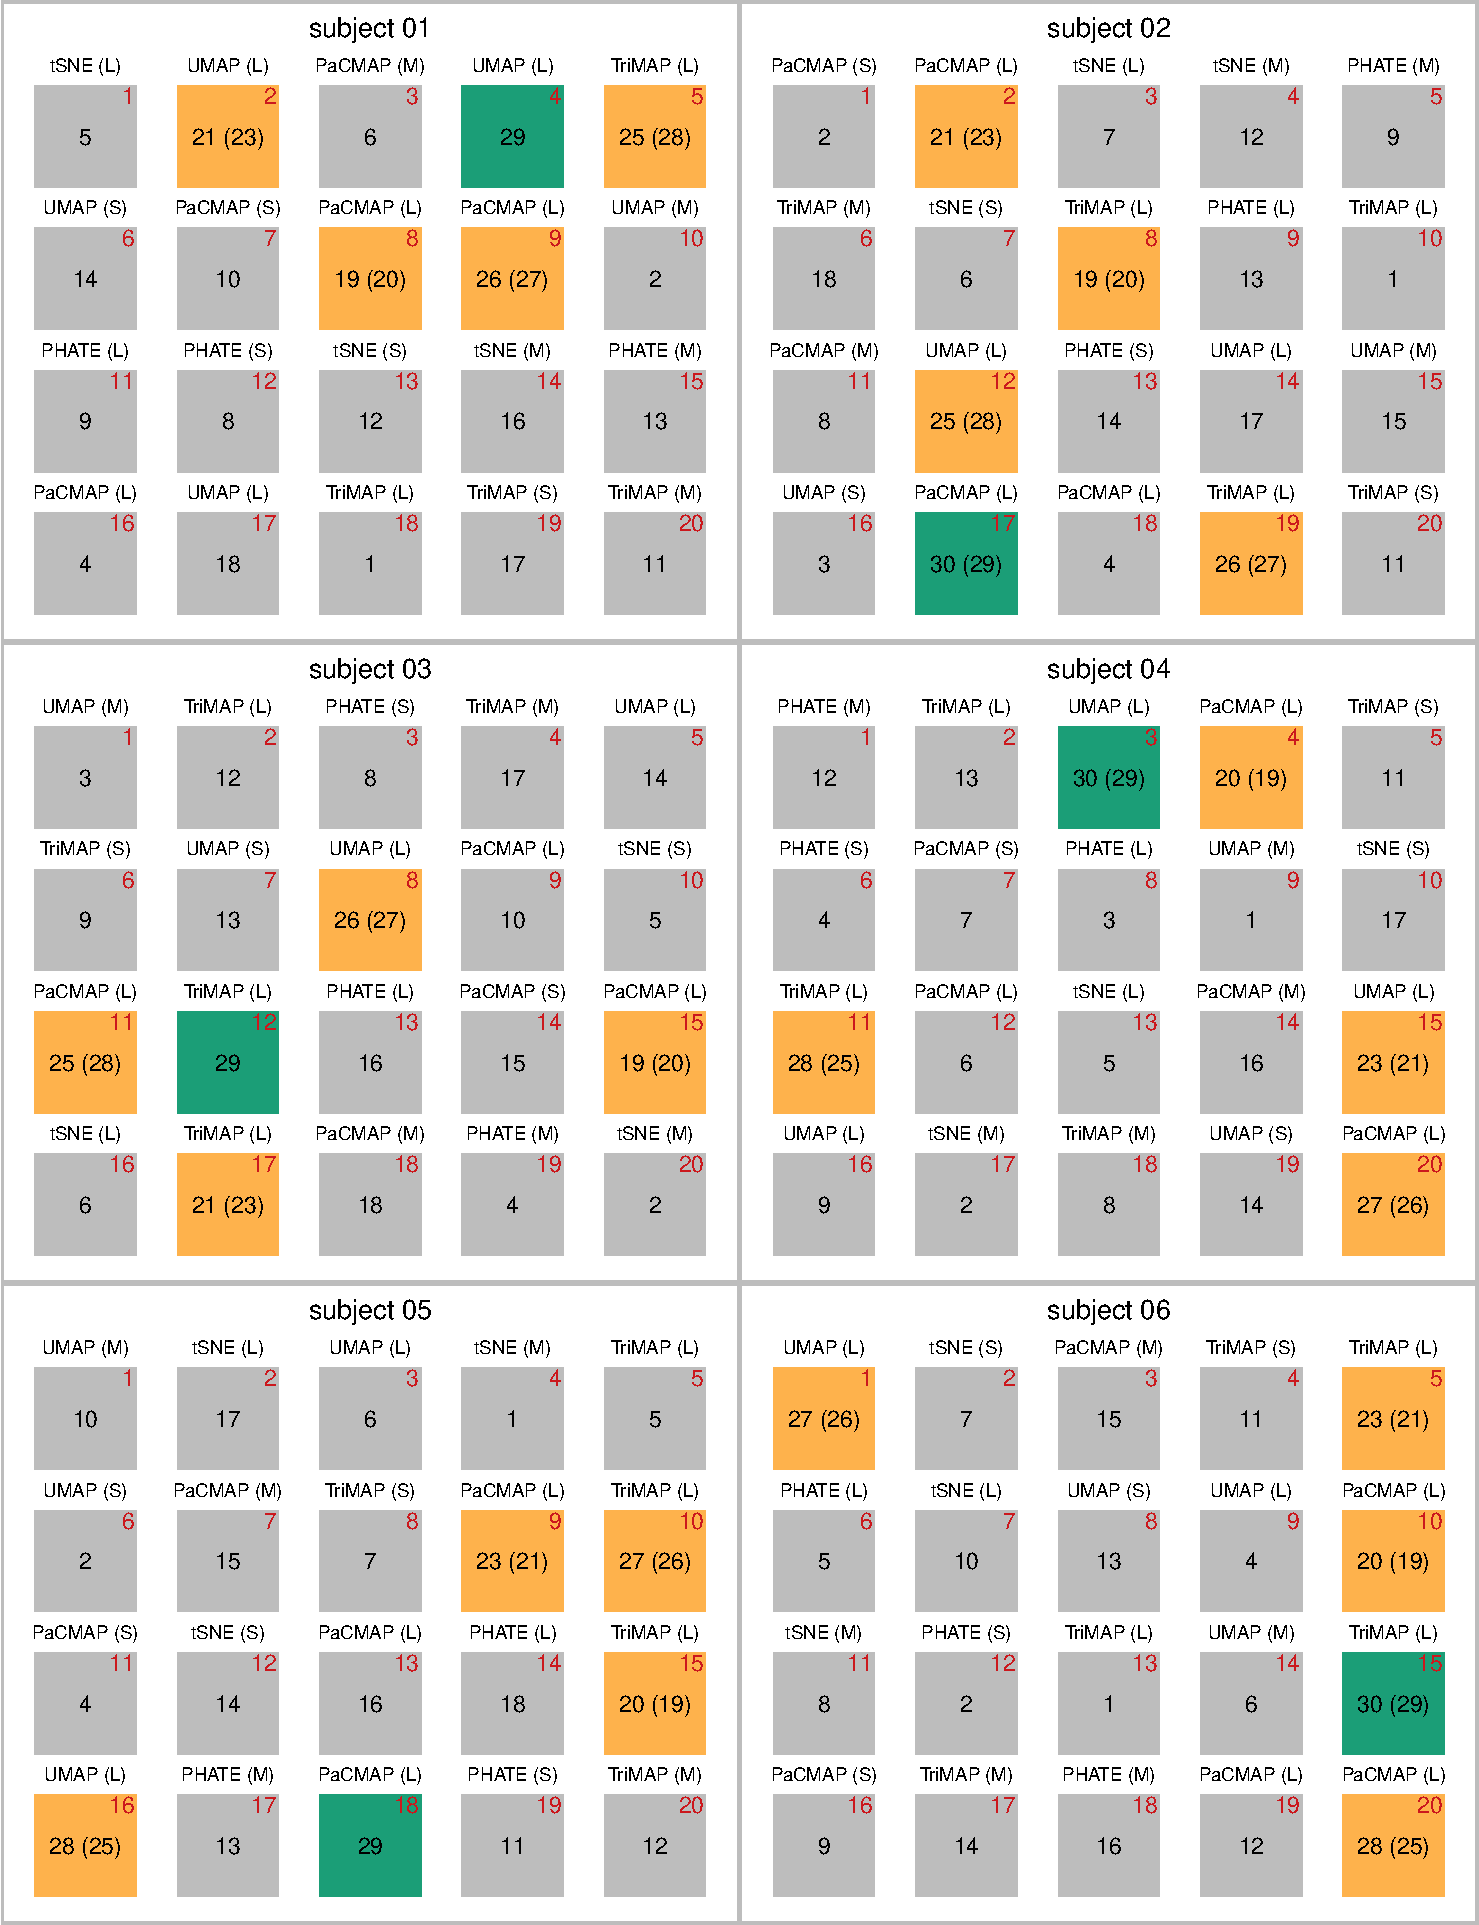
\includegraphics[width=0.9\linewidth,height=\textheight,keepaspectratio]{appendix/C-appC_files/figure-pdf/fig-experiment-design-ds-1.pdf}

}

\caption{\label{fig-experiment-design-ds}The experimental design used
for the study involved six participants. Each small box contains data
structure id in black text. The gray color represents two plots that
display the same data, while the orange color indicates two plots that
show different data. The green color signifies the attention check
trial. If the two plots show different data, the data used in the tour
is mentioned within the brackets. The title of each small box contains
the NLDR method, and within the brackets, the distance scale factor
(\texttt{S} for small, \texttt{M} for medium, and \texttt{L} for large).
The red color text in the top right corner of the small box represents
the attempt.}

\end{figure}%

\section{Data collection process}\label{data-collection-process}

\subsection{Recruite participants}\label{recruite-participants}

Subjects were recruited from Prolific
(\citeproc{ref-palan2018}{\textbf{palan2018?}}), an online platform, to
evaluate the trials. The study expects that the participants are
uninvolved judges with no prior knowledge of the data to avoid
inadvertently affecting results. Potential subjects needed with fluent
in English and have completed at least \(10\) Prolific studies with a
\(98\%\) approval rate. The Prolific server only considers participants
who are age \(18\) and older.

All subjects were trained using three example displays to orient them to
the evaluation trials and provided
\href{https://drive.google.com/file/d/14o-nSjy50Qw2eoQArK5AhjowLIOe6m14/view}{introductory
materials}. All subjects who completed the task were compensated
\(9.96\) GBP per hour for their time via the Prolific payment system.

\subsection{Web application to collect
responses}\label{web-application-to-collect-responses}

The survey web application,
\href{https://ebsmonash.shinyapps.io/web_game/}{Match-a-roo}, is
designed to collect survey responses and demographics using the
\texttt{shiny} (\citeproc{ref-winston2024}{\textbf{winston2024?}})
package in R. Each subject had access to the survey via the shiny.io
server. The first interface of the survey app contained an introduction,
instructions for the survey (Figure~\ref{fig-intro-page}), a consent
form (Figure~\ref{fig-consent}), and buttons to access, for example,
actual trials. Participants can try three examples prior to the study
where the answers were not recorded (Figure~\ref{fig-example}). The
subjects were first asked for their consent to the responses being used
for analysis.

After giving consent, the participant can start the trials. Two visual
displays of data are shown where the data may be the same or different
(Figure~\ref{fig-act}). One of the visual displays is a \gD{} static
plot, and the other is a motion plot made of many \gD{} plots. The
participants were asked to decide whether that data was the same in both
displays and to report their confidence about their choice and any
comments about the answer.

When the participants completed the twenty-three evaluations, they were
asked for their demographics which included preferred pronoun, the
highest level of education achieved, their age category, whether they
used principal component analysis in their work, and whether they
applied NLDR techniques such as tSNE and UMAP (Figure~\ref{fig-demo}).
Finally, the participants need to click on prolific URL
(\href{https://app.prolific.co/submissions/complete?cc=CLDDOZ10}{https://app.prolific.co/submissions/})
to redirect back to the Prolific app (Figure~\ref{fig-end}).

\begin{figure}

\centering{

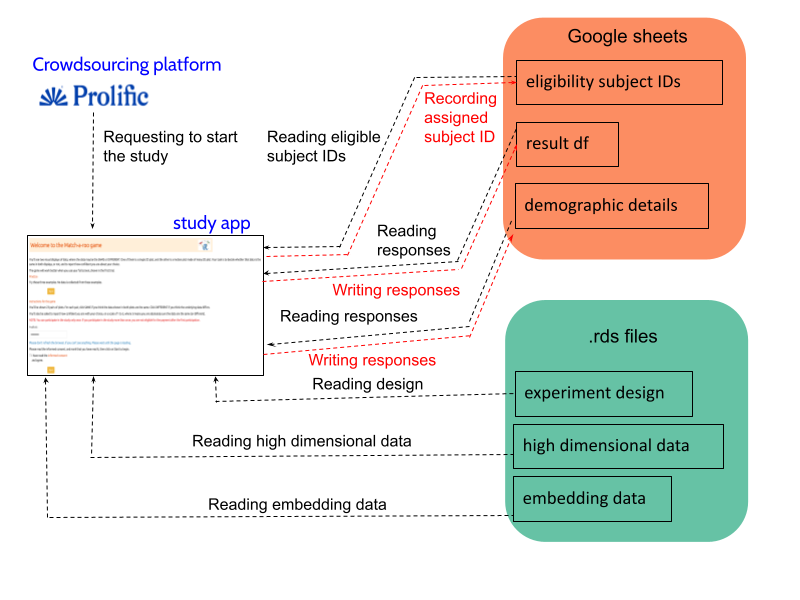
\includegraphics[width=1\linewidth,height=\textheight,keepaspectratio]{appendix/../figures/vis-exp/experiment.png}

}

\caption{\label{fig-exp-setup}Diagram of online experiment setup.}

\end{figure}%

\begin{figure}

\centering{

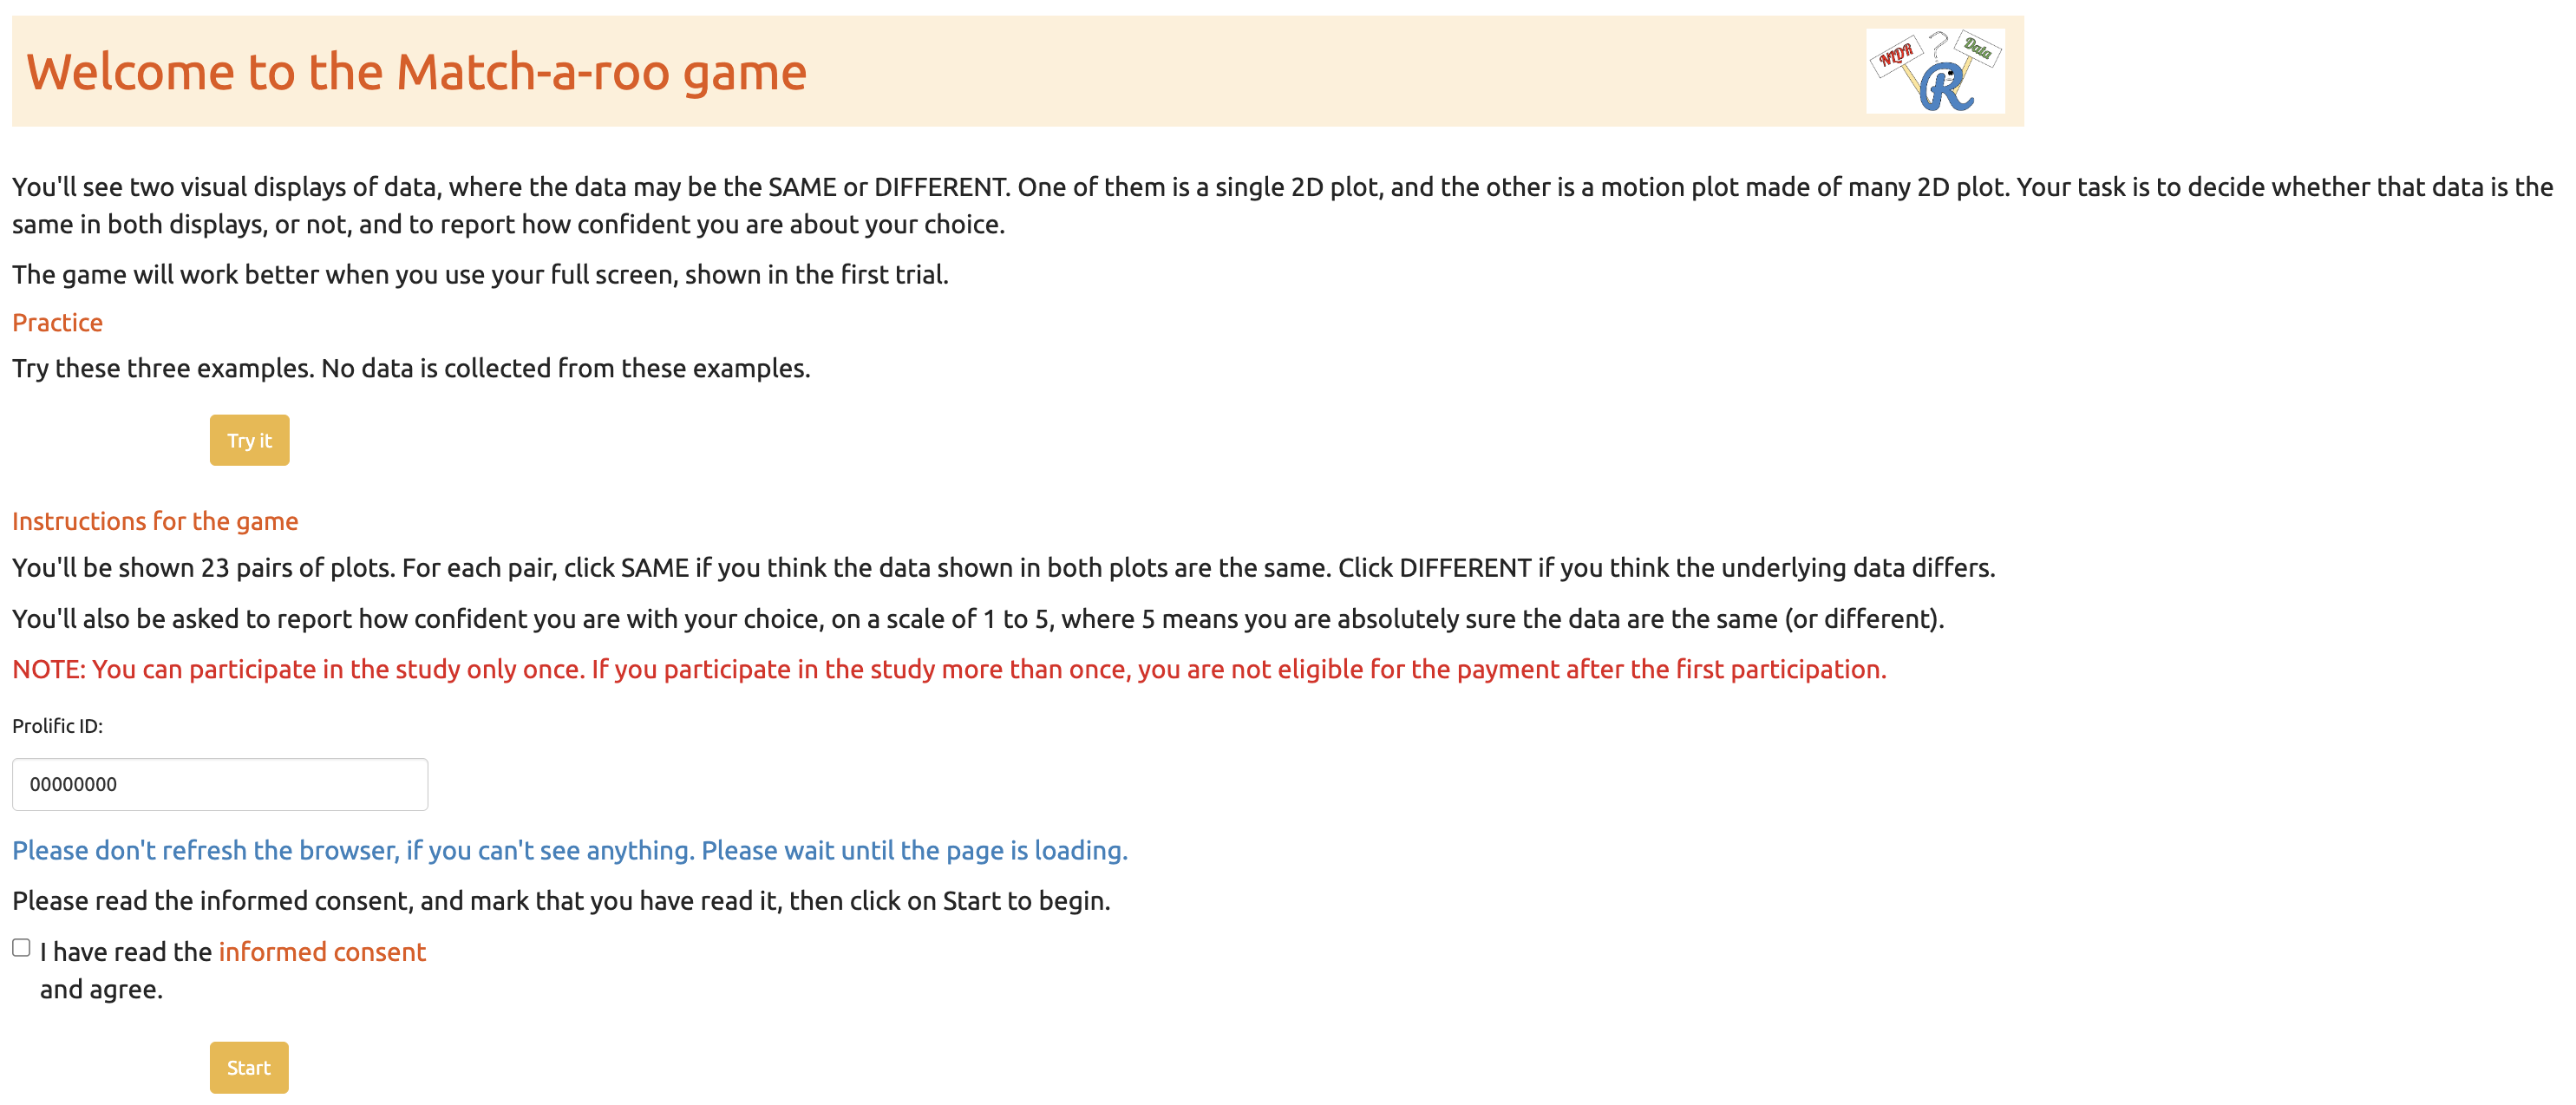
\includegraphics[width=1\linewidth,height=\textheight,keepaspectratio]{appendix/../figures/vis-exp/introduction.png}

}

\caption{\label{fig-intro-page}The introduction page of the study app.}

\end{figure}%

\begin{figure}

\centering{


\includegraphics[width=1\linewidth,height=\textheight,keepaspectratio]{appendix/../figures/vis-exp/consent.png}

}

\caption{\label{fig-consent}The consent form provided in the study app.}

\end{figure}%

\begin{figure}

\centering{

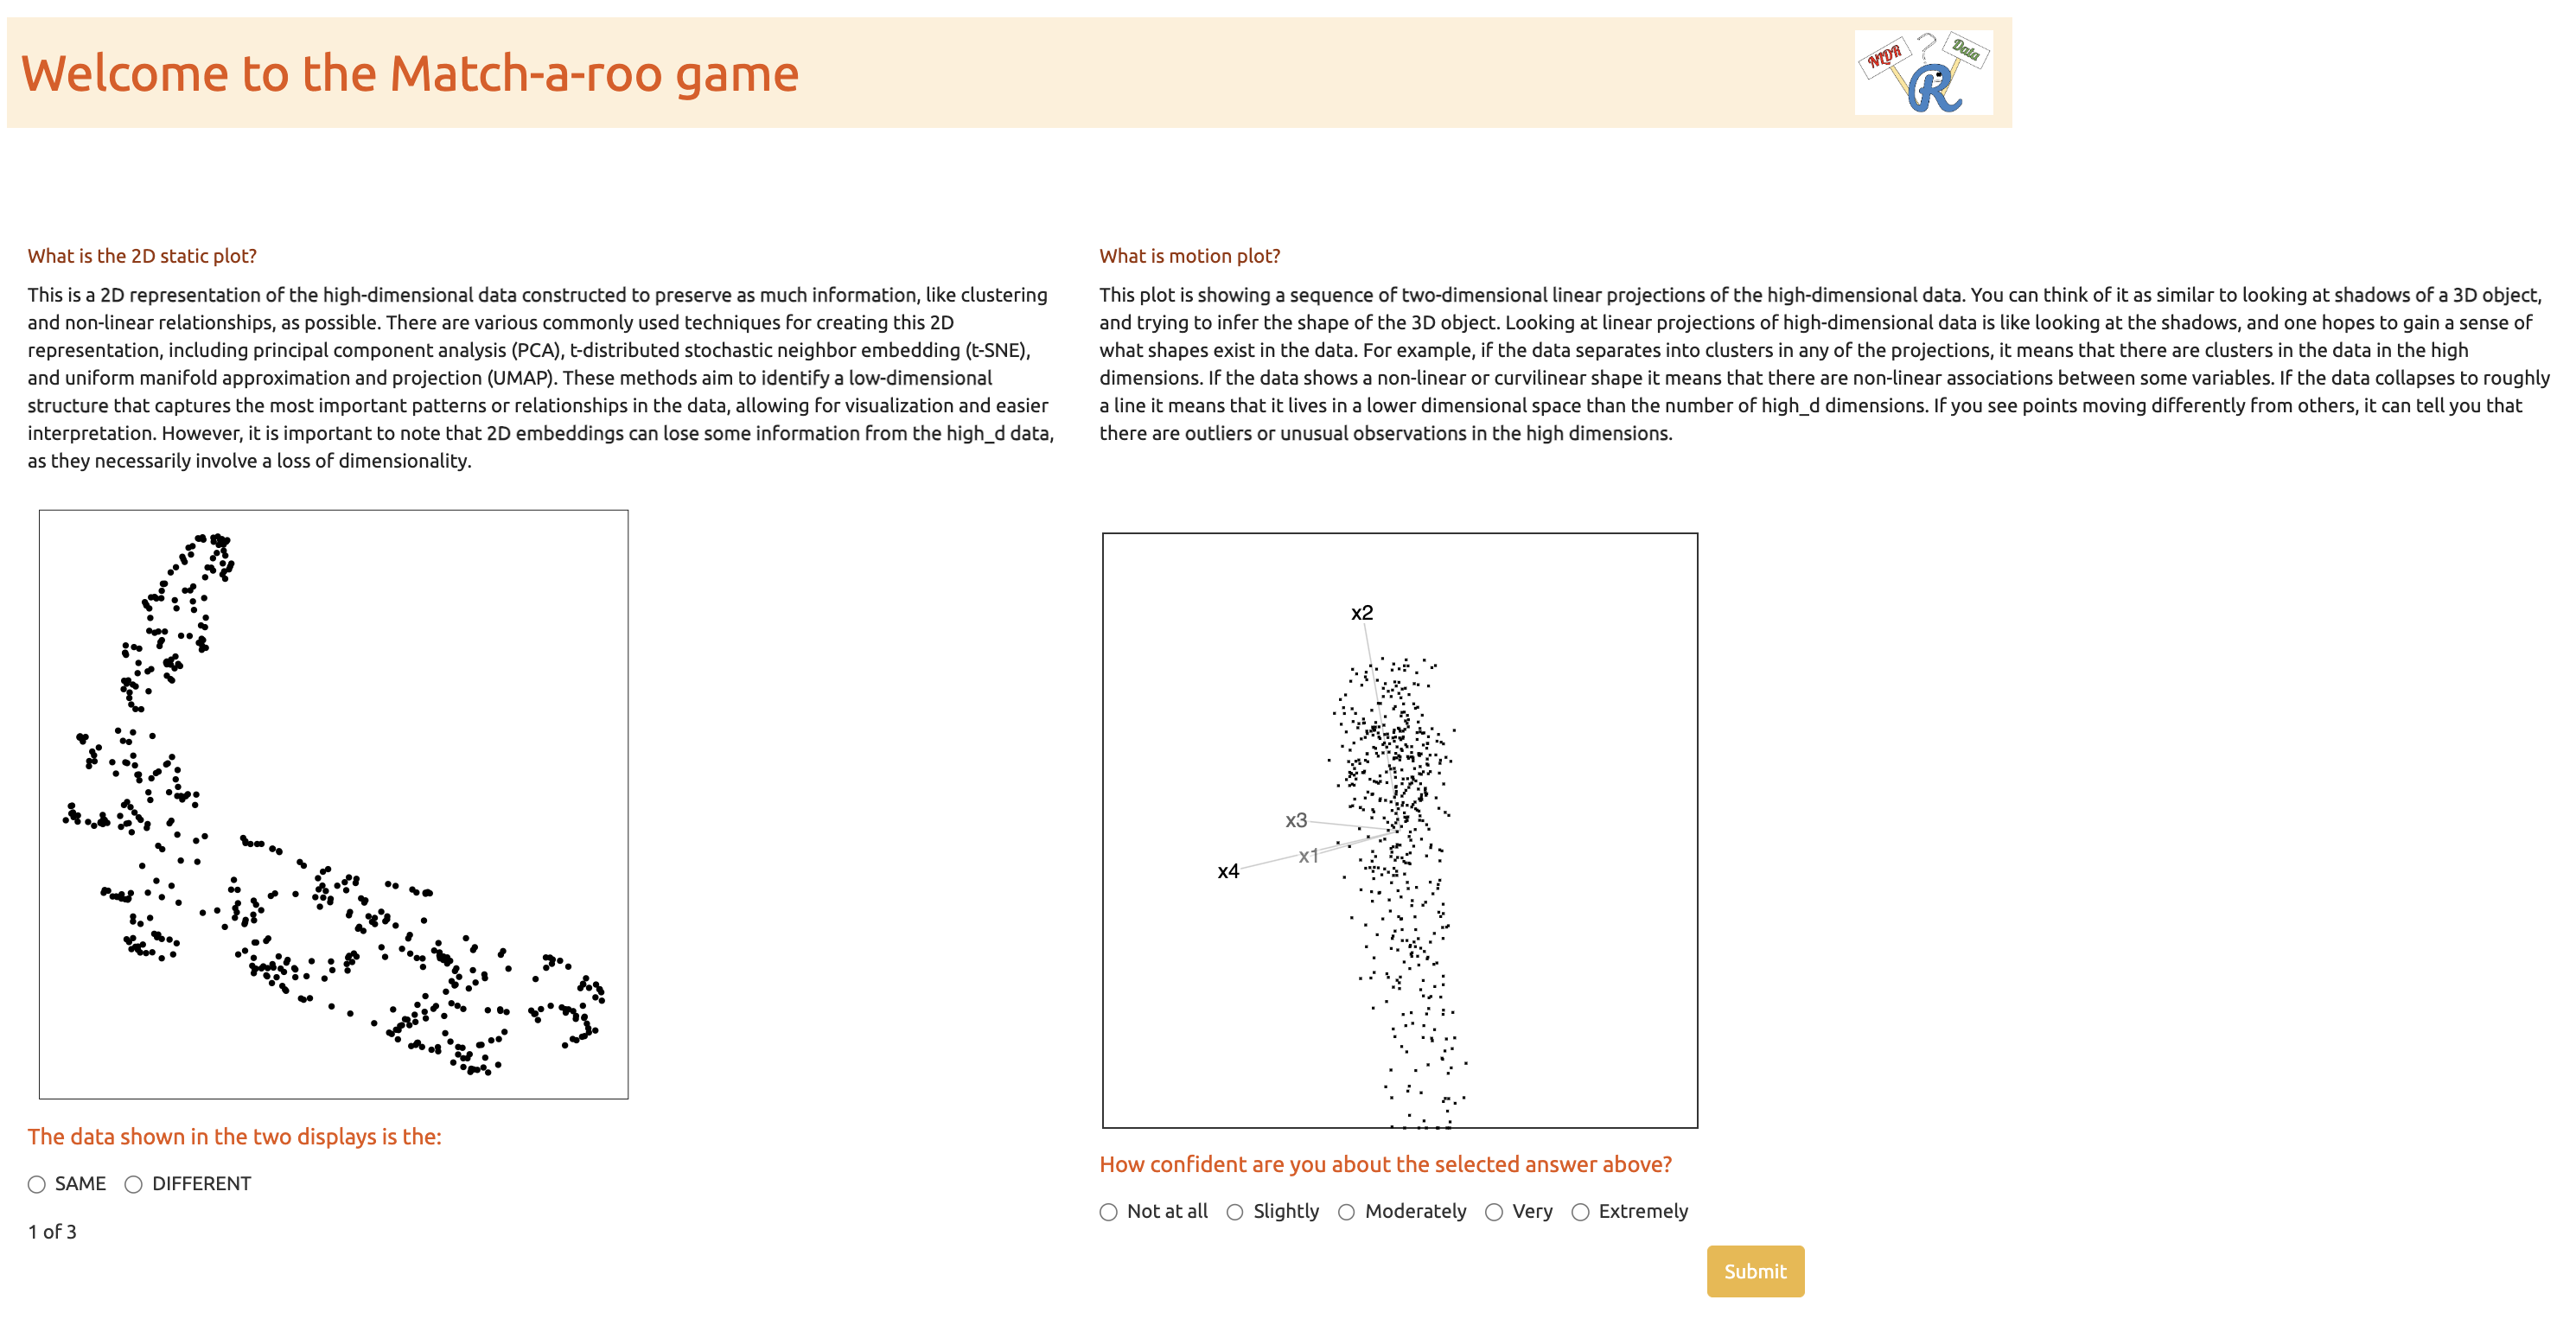
\includegraphics[width=1\linewidth,height=\textheight,keepaspectratio]{appendix/../figures/vis-exp/example.png}

}

\caption{\label{fig-example}The example trial page of the study app.}

\end{figure}%

\begin{figure}

\centering{

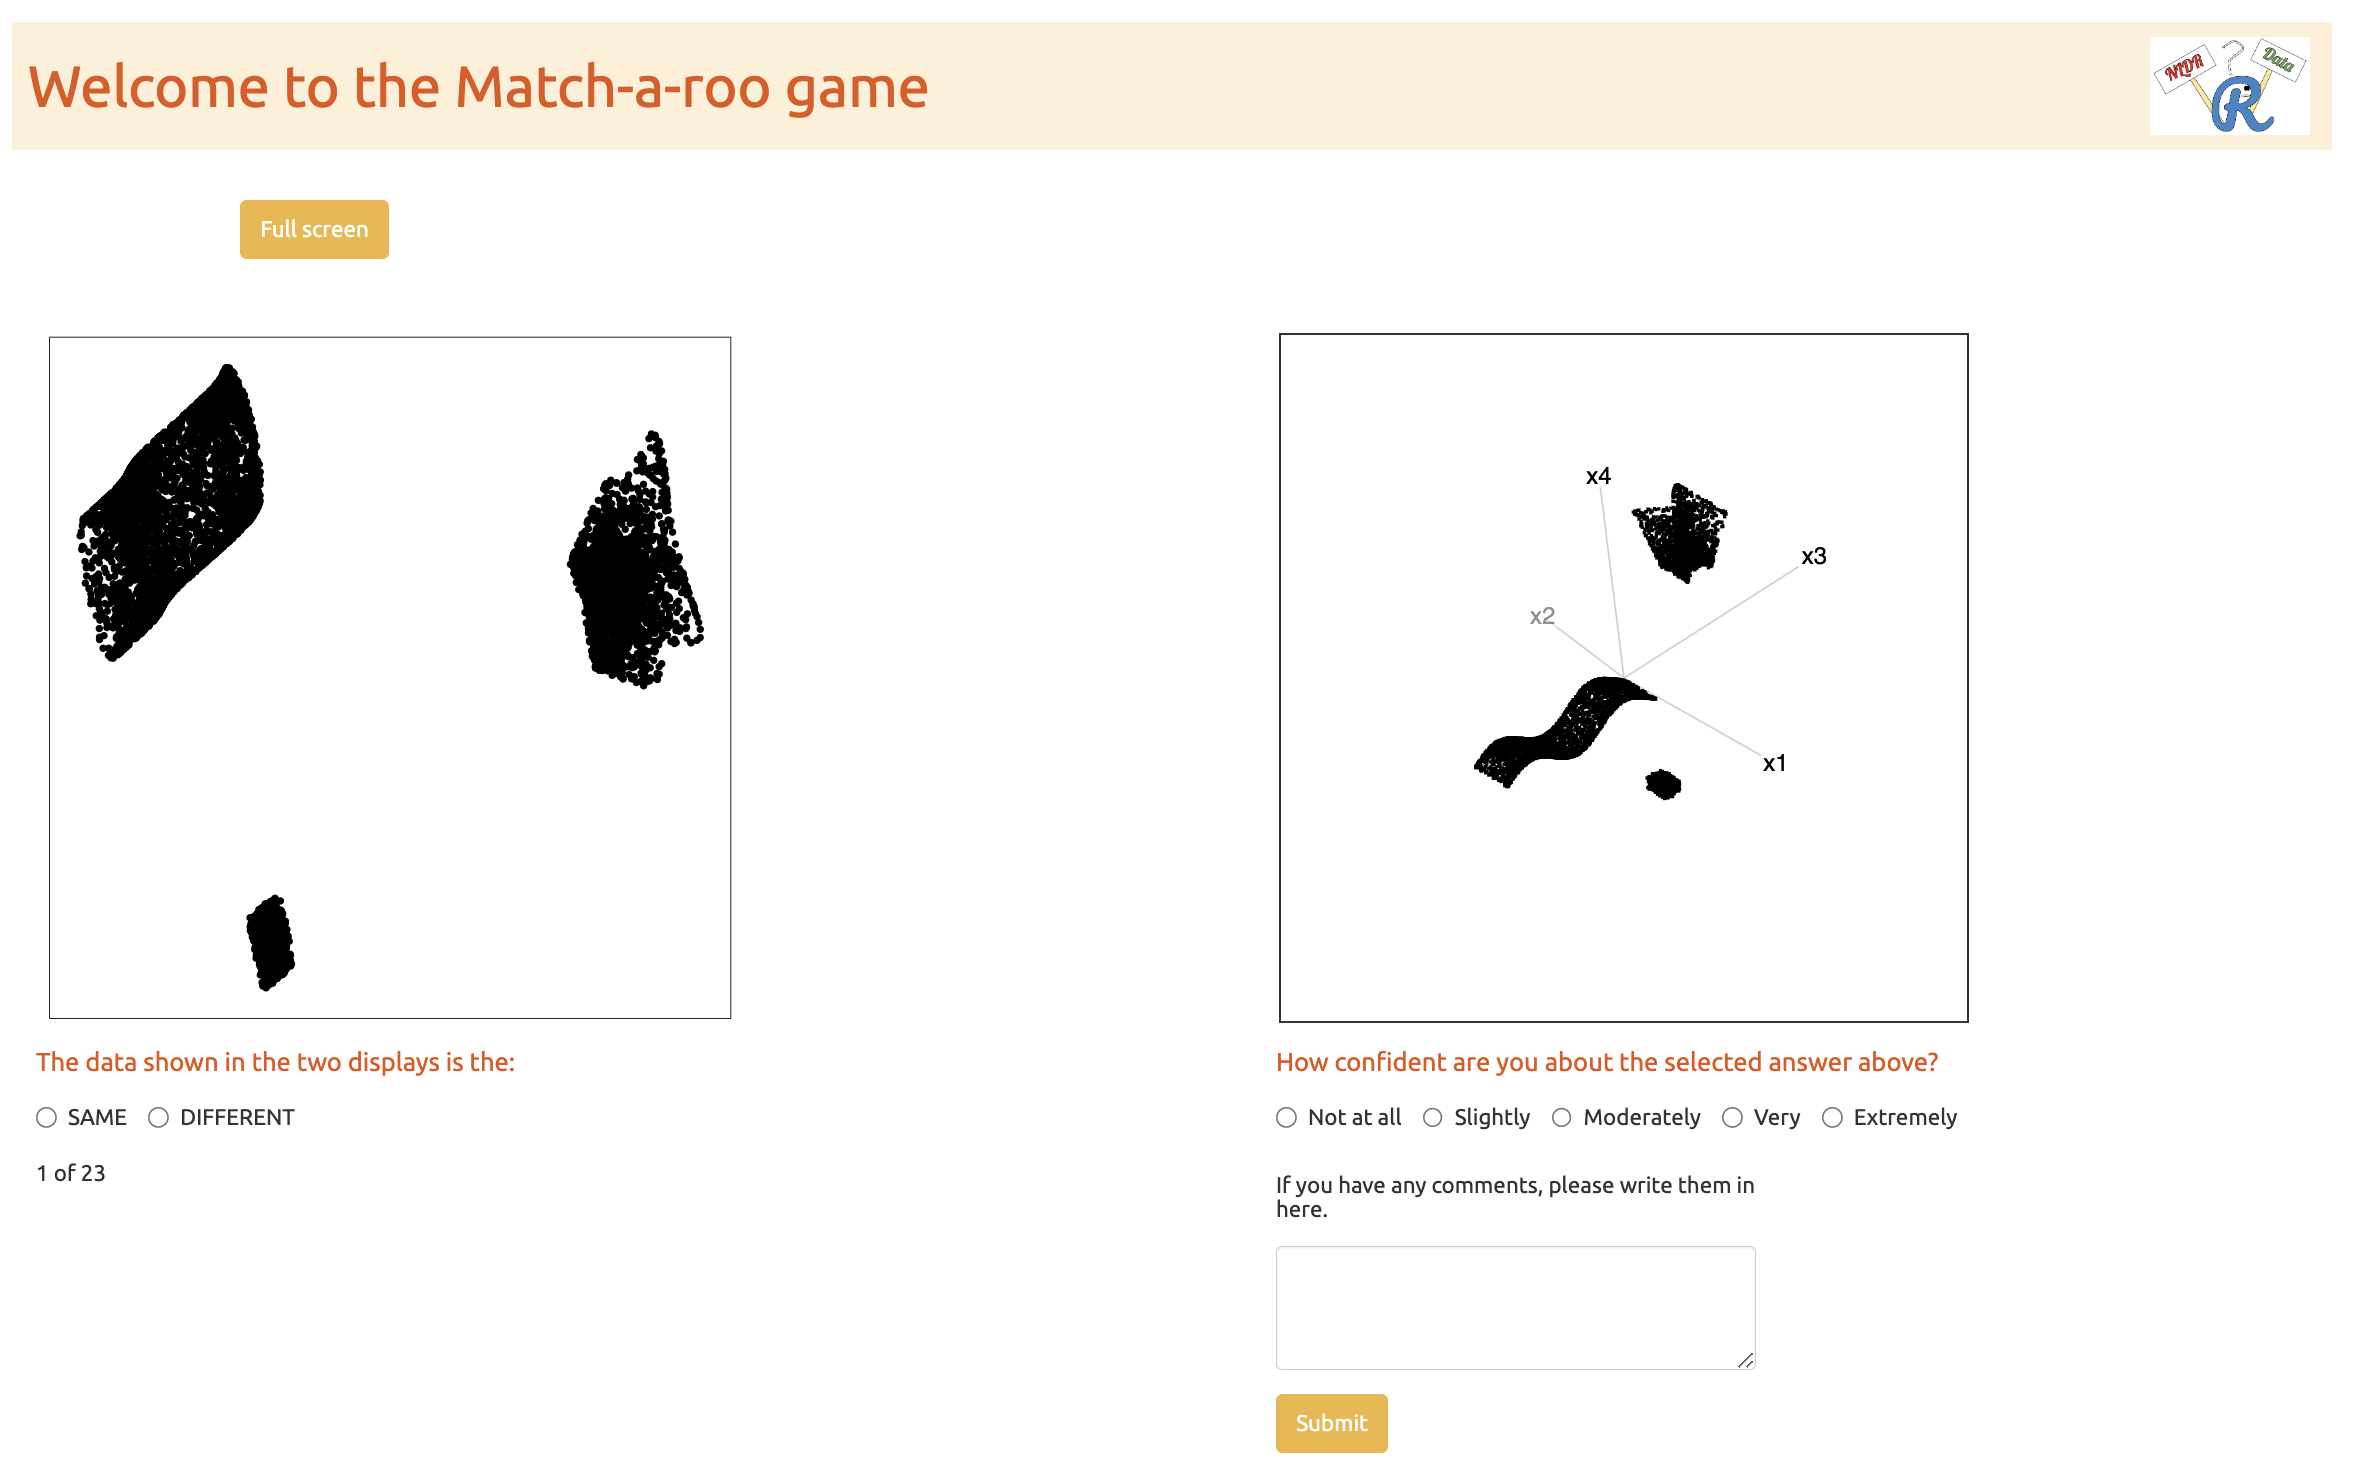
\includegraphics[width=1\linewidth,height=\textheight,keepaspectratio]{appendix/../figures/vis-exp/attempt.png}

}

\caption{\label{fig-act}The actual trial page of the study app.}

\end{figure}%

\begin{figure}

\centering{

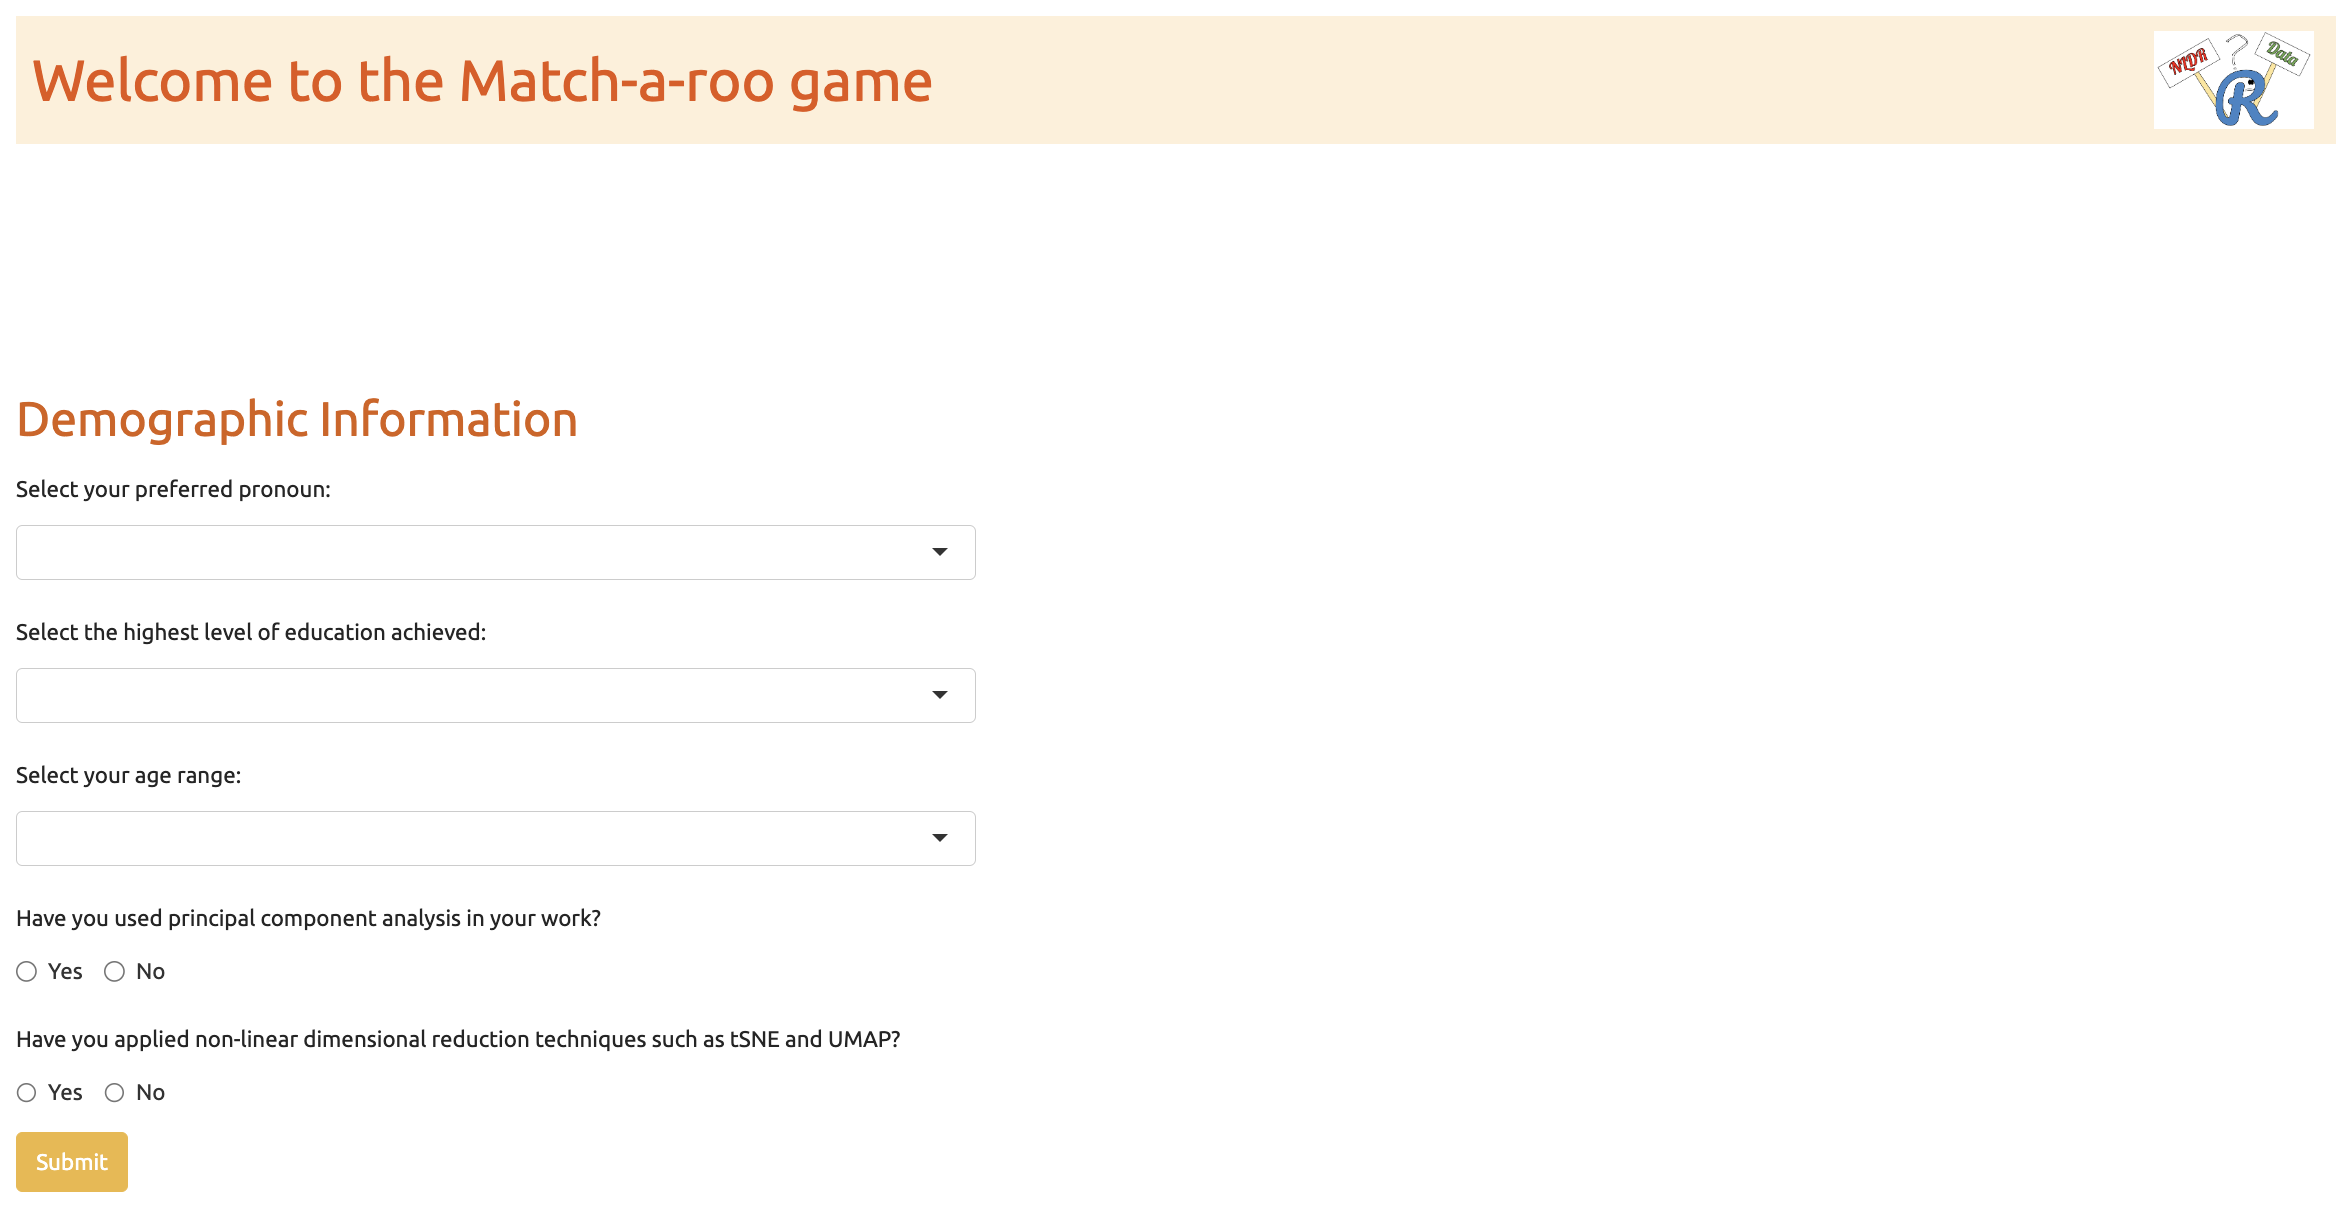
\includegraphics[width=1\linewidth,height=\textheight,keepaspectratio]{appendix/../figures/vis-exp/demographics.png}

}

\caption{\label{fig-demo}The demographics page of the study app.}

\end{figure}%

\begin{figure}

\centering{


\includegraphics[width=1\linewidth,height=\textheight,keepaspectratio]{appendix/../figures/vis-exp/end_page.png}

}

\caption{\label{fig-end}The end page of the study app.}

\end{figure}%

Once a participant starts the study (Figure~\ref{fig-exp-setup}), the
``eligibility\_subject\_IDs'' Google Sheet is connected and read in the
Shiny app to identify which subject IDs have not yet been assigned to
anyone, as indicated by the ``used'' column. If the ``used'' column is
marked as NA, it means that the subject ID has not been assigned.

After identifying the eligible subject IDs, one is randomly assigned to
the participant, and ``1'' is recorded in the ``used'' column
corresponding to that subject ID. This subject ID will later assist in
connecting the experiment design, high-dimensional data, and embedding
data.

Once a subject ID is allocated to a participant, the experiment design
data is loaded, and the relevant attempts, data structure, and methods
are presented to the participant. This process continues until the
participant completes all attempts. After determining the data structure
and methods, the relevant high-dimensional and embedding data is loaded
from ``high\_d\_data\_three\_clust\_all.rds'' and
``embedding\_data\_three\_clust\_all.rds,'' respectively, and displayed
in both motion and \gD{} static plots.

Once the participant records their answers, a new row is added to the
``result\_df'' Google Sheet with their responses. This continues until
the participant finishes the study. Finally, after completing the
evaluations, participants are asked to fill out a demographics
questionnaire. Their responses are then recorded in a new row of the
``demographic\_details'' Google Sheet.

\section{Analysis of results relative to data collection
process}\label{analysis-of-results-relative-to-data-collection-process}

\subsection{Data cleaning}\label{data-cleaning}

The initial step in the data cleaning process involves the selection of
subjects who have completed the requisite twenty-three trials, including
the demographics and the attention check trial. Participants who
exceeded the average time of 5-10 minutes were excluded, as determined
from the pilot study. Following this, individuals who didn't accurately
detect the attention check trial were also removed. Furthermore, the
attention check trials were removed, as they did not contribute to the
further analyses. Finally, the collected data set is further refined by
filtering out all the responses, which showed the same data structures
in \gD{} static and motion plots.

\subsection{Demographics}\label{demographics}

Along with the responses to the trials, we have collected a series of
demographic information including preferred pronoun, age range category,
education background, and previous experience in PCA and Non-linear
dimension reduction techniques. Table~\ref{tbl-pronoun},
Table~\ref{tbl-age}, Table~\ref{tbl-education}, Table~\ref{tbl-pca}, and
Table~\ref{tbl-nldr} provide summaries of the demographic data.

XXX After collecting data need to add interpretations

\begin{table}

\caption{\label{tbl-pronoun}Summary of the pronoun distribution of
participants recruited for this study.}

\centering{

\centering
\resizebox{\ifdim\width>\linewidth\linewidth\else\width\fi}{!}{
\begin{tabular}{lrrrr}
\toprule
Pronoun & Period I & Period II & Total & \%\\
\midrule
he/him & 7 & 54 & 61 & 48.03\\
she/her & 11 & 53 & 64 & 50.39\\
they/them & 0 & 2 & 2 & 1.57\\
Total & 18 & 109 & 127 & 100.00\\
\bottomrule
\end{tabular}}

}

\end{table}%

\begin{table}

\caption{\label{tbl-age}Summary of the age distribution of participants
recruited for this study.}

\centering{

\centering
\resizebox{\ifdim\width>\linewidth\linewidth\else\width\fi}{!}{
\begin{tabular}{lrrrr}
\toprule
Age group & Period I & Period II & Total & \%\\
\midrule
18 - 24 & 3 & 23 & 26 & 20.47\\
25 - 34 & 9 & 36 & 45 & 35.43\\
35 - 44 & 3 & 22 & 25 & 19.69\\
45 - 54 & 1 & 12 & 13 & 10.24\\
Over 55 & 2 & 16 & 18 & 14.17\\
\addlinespace
Total & 18 & 109 & 127 & 100.00\\
\bottomrule
\end{tabular}}

}

\end{table}%

\begin{table}

\caption{\label{tbl-education}Summary of the educational distribution of
participants recruited for this study.}

\centering{

\centering
\resizebox{\ifdim\width>\linewidth\linewidth\else\width\fi}{!}{
\begin{tabular}{lrrrr}
\toprule
Education & Period I & Period II & Total & \%\\
\midrule
Completed some undergraduate courses & 4 & 23 & 27 & 21.26\\
Did not complete high school & 0 & 4 & 4 & 3.15\\
Higher degree master or doctorate & 3 & 31 & 34 & 26.77\\
Prefer not to answer & 3 & 2 & 5 & 3.94\\
Undergraduate degree (A bachelor) & 8 & 49 & 57 & 44.88\\
\addlinespace
Total & 18 & 109 & 127 & 100.00\\
\bottomrule
\end{tabular}}

}

\end{table}%

\begin{table}

\caption{\label{tbl-pca}Summary of the previous experience in PCA of
participants recruited for this study.}

\centering{

\centering
\resizebox{\ifdim\width>\linewidth\linewidth\else\width\fi}{!}{
\begin{tabular}{lrrrr}
\toprule
Experience with PCA & Period I & Period II & Total & \%\\
\midrule
No & 15 & 92 & 107 & 84.25\\
Yes & 3 & 17 & 20 & 15.75\\
Total & 18 & 109 & 127 & 100.00\\
\bottomrule
\end{tabular}}

}

\end{table}%

\begin{table}

\caption{\label{tbl-nldr}Summary of the previous experience in
Non-linear dimension reduction techniques of participants recruited for
this study.}

\centering{

\centering
\resizebox{\ifdim\width>\linewidth\linewidth\else\width\fi}{!}{
\begin{tabular}{lrrrr}
\toprule
Experience with NLDR & Period I & Period II & Total & \%\\
\midrule
No & 15 & 95 & 110 & 86.61\\
Yes & 3 & 14 & 17 & 13.39\\
Total & 18 & 109 & 127 & 100.00\\
\bottomrule
\end{tabular}}

}

\end{table}%

XXX Add plot with time Vs attempt for the subjects XXX Check is there
any specific pattern for each demographics with their answers (eg: Male
correctly identify more, or in which region\ldots)

\section{Non-attention check data
generation}\label{non-attention-check-data-generation}

The process of generating non-attention check data involves several
steps. First, we generate clustering data using a distance scale factor
of \(1\), with sample size of \(7500\), no noise dimensions, and no
background noise. Next, the data generated with a distance scale factor
of \(1\) and a sample size of \(7500\) is used to create data with
different distance scale factors (\(0.1\)) (\textbf{?@alg-gen-diff-sf}).

\begin{longtable}{>{\raggedright\arraybackslash}p{5em}>{\raggedleft\arraybackslash}p{3em}>{\raggedleft\arraybackslash}p{3em}>{\raggedleft\arraybackslash}p{3em}>{\raggedleft\arraybackslash}p{3em}>{\raggedleft\arraybackslash}p{3em}>{\raggedleft\arraybackslash}p{3em}>{\raggedleft\arraybackslash}p{3em}}

\caption{\label{tbl-dist-centroid-four-clust}\(4\text{-}D\) distances
between centroid points in three clusters.}

\tabularnewline

\toprule
structure & dist\_sf & dist12 & dist13 & dist23 & prop12 & prop13 & prop23\\
\midrule
three\_clust\_01 & 0.1 & 0.27 & 0.48 & 0.22 & 0.1 & 0.1 & 0.1\\
three\_clust\_01 & 0.6 & 1.32 & 2.34 & 2.07 & 0.6 & 0.6 & 0.6\\
three\_clust\_01 & 1.0 & 2.16 & 3.98 & 3.58 & 1.0 & 1.0 & 1.0\\
three\_clust\_02 & 0.1 & 0.28 & 0.32 & 0.25 & 0.1 & 0.1 & 0.1\\
three\_clust\_02 & 0.6 & 1.31 & 2.49 & 2.14 & 0.6 & 0.6 & 0.6\\
\addlinespace
three\_clust\_02 & 1.0 & 2.16 & 3.94 & 3.53 & 1.0 & 1.0 & 1.0\\
three\_clust\_03 & 0.1 & 0.30 & 0.40 & 0.28 & 0.1 & 0.1 & 0.1\\
three\_clust\_03 & 0.6 & 1.26 & 2.47 & 2.26 & 0.6 & 0.6 & 0.6\\
three\_clust\_03 & 1.0 & 2.17 & 3.91 & 3.49 & 1.0 & 1.0 & 1.0\\
three\_clust\_04 & 0.1 & 0.28 & 0.53 & 0.48 & 0.1 & 0.1 & 0.1\\
\addlinespace
three\_clust\_04 & 0.6 & 1.39 & 2.35 & 2.20 & 0.6 & 0.6 & 0.6\\
three\_clust\_04 & 1.0 & 2.16 & 3.93 & 3.51 & 1.0 & 1.0 & 1.0\\
three\_clust\_05 & 0.1 & 0.27 & 0.27 & 0.24 & 0.1 & 0.1 & 0.1\\
three\_clust\_05 & 0.6 & 1.35 & 2.41 & 2.23 & 0.6 & 0.6 & 0.6\\
three\_clust\_05 & 1.0 & 2.16 & 4.04 & 3.64 & 1.0 & 1.0 & 1.0\\
\addlinespace
three\_clust\_06 & 0.1 & 0.31 & 0.39 & 0.36 & 0.1 & 0.1 & 0.1\\
three\_clust\_06 & 0.6 & 1.33 & 2.48 & 2.12 & 0.6 & 0.6 & 0.6\\
three\_clust\_06 & 1.0 & 2.17 & 3.91 & 3.48 & 1.0 & 1.0 & 1.0\\
three\_clust\_07 & 0.1 & 0.18 & 0.33 & 0.32 & 0.1 & 0.1 & 0.1\\
three\_clust\_07 & 0.6 & 1.24 & 2.37 & 2.09 & 0.6 & 0.6 & 0.6\\
\addlinespace
three\_clust\_07 & 1.0 & 2.18 & 3.95 & 3.53 & 1.0 & 1.0 & 1.0\\
three\_clust\_08 & 0.1 & 0.18 & 0.53 & 0.51 & 0.1 & 0.1 & 0.1\\
three\_clust\_08 & 0.6 & 1.27 & 2.31 & 2.18 & 0.6 & 0.6 & 0.6\\
three\_clust\_08 & 1.0 & 2.08 & 4.01 & 3.63 & 1.0 & 1.0 & 1.0\\
three\_clust\_09 & 0.1 & 0.30 & 0.24 & 0.23 & 0.1 & 0.1 & 0.1\\
\addlinespace
three\_clust\_09 & 0.6 & 1.26 & 2.32 & 2.08 & 0.6 & 0.6 & 0.6\\
three\_clust\_09 & 1.0 & 2.17 & 4.06 & 3.65 & 1.0 & 1.0 & 1.0\\
three\_clust\_10 & 0.1 & 0.21 & 0.48 & 0.41 & 0.1 & 0.1 & 0.1\\
three\_clust\_10 & 0.6 & 1.36 & 2.34 & 2.14 & 0.6 & 0.6 & 0.6\\
three\_clust\_10 & 1.0 & 2.19 & 4.07 & 3.66 & 1.0 & 1.0 & 1.0\\
\addlinespace
three\_clust\_11 & 0.1 & 0.25 & 0.58 & 0.53 & 0.1 & 0.1 & 0.1\\
three\_clust\_11 & 0.6 & 1.27 & 2.44 & 2.22 & 0.6 & 0.6 & 0.6\\
three\_clust\_11 & 1.0 & 2.15 & 3.99 & 3.59 & 1.0 & 1.0 & 1.0\\
three\_clust\_12 & 0.1 & 0.26 & 0.54 & 0.48 & 0.1 & 0.1 & 0.1\\
three\_clust\_12 & 0.6 & 1.27 & 2.47 & 2.24 & 0.6 & 0.6 & 0.6\\
\addlinespace
three\_clust\_12 & 1.0 & 2.15 & 3.92 & 3.51 & 1.0 & 1.0 & 1.0\\
three\_clust\_13 & 0.1 & 0.31 & 0.33 & 0.24 & 0.1 & 0.1 & 0.1\\
three\_clust\_13 & 0.6 & 1.28 & 2.47 & 2.24 & 0.6 & 0.6 & 0.6\\
three\_clust\_13 & 1.0 & 2.17 & 3.91 & 3.49 & 1.0 & 1.0 & 1.0\\
three\_clust\_14 & 0.1 & 0.18 & 0.58 & 0.52 & 0.1 & 0.1 & 0.1\\
\addlinespace
three\_clust\_14 & 0.6 & 1.30 & 2.23 & 2.04 & 0.6 & 0.6 & 0.6\\
three\_clust\_14 & 1.0 & 2.19 & 3.95 & 3.52 & 1.0 & 1.0 & 1.0\\
three\_clust\_15 & 0.1 & 0.26 & 0.37 & 0.35 & 0.1 & 0.1 & 0.1\\
three\_clust\_15 & 0.6 & 1.29 & 2.52 & 2.36 & 0.6 & 0.6 & 0.6\\
three\_clust\_15 & 1.0 & 2.15 & 4.05 & 3.66 & 1.0 & 1.0 & 1.0\\
\addlinespace
three\_clust\_16 & 0.1 & 0.27 & 0.49 & 0.25 & 0.1 & 0.1 & 0.1\\
three\_clust\_16 & 0.6 & 1.35 & 2.25 & 2.12 & 0.6 & 0.6 & 0.6\\
three\_clust\_16 & 1.0 & 2.16 & 3.87 & 3.45 & 1.0 & 1.0 & 1.0\\
three\_clust\_17 & 0.1 & 0.18 & 0.35 & 0.22 & 0.1 & 0.1 & 0.1\\
three\_clust\_17 & 0.6 & 1.27 & 2.48 & 2.23 & 0.6 & 0.6 & 0.6\\
\addlinespace
three\_clust\_17 & 1.0 & 2.19 & 4.03 & 3.62 & 1.0 & 1.0 & 1.0\\
three\_clust\_18 & 0.1 & 0.20 & 0.25 & 0.23 & 0.1 & 0.1 & 0.1\\
three\_clust\_18 & 0.6 & 1.35 & 2.37 & 2.23 & 0.6 & 0.6 & 0.6\\
three\_clust\_18 & 1.0 & 2.10 & 4.01 & 3.62 & 1.0 & 1.0 & 1.0\\
\bottomrule

\end{longtable}

\section{Non-linear dimension reduction data
generation}\label{non-linear-dimension-reduction-data-generation}

Dimension reduction data generation is performed using various methods:
tSNE ((\citeproc{ref-algo-gen-tsne}{\textbf{algo-gen-tsne?}})), UMAP
((\citeproc{ref-algo-gen-umap}{\textbf{algo-gen-umap?}})), PHATE
((\citeproc{ref-algo-gen-phate}{\textbf{algo-gen-phate?}})), PaCMAP
((\citeproc{ref-algo-gen-pacmap}{\textbf{algo-gen-pacmap?}})), and
TriMAP ((\citeproc{ref-algo-gen-trimap}{\textbf{algo-gen-trimap?}})) on
each high-dimensional dataset, which are then combined at the end.

\chapter{Appendix to ``Development of an interactive and dynamic
graphics system for NLDR users''}\label{sec-appendix-c3}




\end{document}
